\documentclass[a4j,12pt]{jreport}
\makeatletter
%\voffset=0in
%\headheight=0pt
%\headsep=0pt
%\textheight=672pt
%\footskip=24pt

\usepackage{url}
\usepackage{jtygm}
\usepackage{ascmac}
\usepackage[dvips]{graphicx}
\usepackage{amsmath,amssymb}
\usepackage{multicol}
\usepackage{listings}
\usepackage{makeidx}
\usepackage{ccaption}
\usepackage{here}
\usepackage{subfigure}
\usepackage{enumerate}
\usepackage{color}
\usepackage{fancybox}
\usepackage[margin=2.5cm,head=0cm,headsep=0cm]{geometry}


\renewcommand{\postchaptername}{講}
\renewcommand{\lstlistingname}{リスト}

\newcommand{\minisec}[1]{
\subsubsection{【#1】}
}

% 付録の始まり
\newcommand{\beginappendix}{
  % 章番号の書式変更
  \setcounter{chapter}{0}
  \renewcommand{\prechaptername}{付録}
  \renewcommand{\postchaptername}{} 
  \renewcommand{\thechapter}{\@Alph\c@chapter}
  \renewcommand{\thesection}{\@Alph\c@chapter.\@arabic\c@section}
  \renewcommand{\thesubsection}{\@Alph\c@chapter.\@arabic\c@section.\@arabic\c@subsection}
}

%図番号の書式変更
  \renewcommand{\thefigure}{%
  \thechapter.\arabic{figure}}
  \@addtoreset{figure}{chapter}
\makeatother


\newcommand{\ruby}[2]{%
\leavevmode
\setbox0=\hbox{#1}%
\setbox1=\hbox{\tiny #2}%
\ifdim\wd0>\wd1 \dimen0=\wd0 \else \dimen0=\wd1 \fi
\hbox{%
\kanjiskip=0pt plus 2fil
\xkanjiskip=0pt plus 2fil
\vbox{%
\hbox to \dimen0{%
\tiny \hfil#2\hfil}%
\nointerlineskip
\hbox to \dimen0{\mathstrut\hfil#1\hfil}}}}

\makeatletter
\lstset{% 
language={C}, 
frame=trbl,% 
basicstyle={\small},% 
identifierstyle={\small},% 
commentstyle={\small\ttfamily},% 
keywordstyle={\small\bfseries},% 
ndkeywordstyle={\small},% 
stringstyle={\small\ttfamily}, 
tabsize=2,
breaklines=true, 
frame=none,
columns=[l]{fullflexible},% 
numbers=left,% 
xrightmargin=0zw,% 
xleftmargin=3zw,% 
numberstyle={\scriptsize},% 
stepnumber=1, 
numbersep=1zw,% 
backgroundcolor={\color[gray]{.90}},
} 

%footnoteにおいてverbを有効にする設定
\long\def\@footnotetext{%
  \insert\footins\bgroup
    \normalfont\footnotesize
    \interlinepenalty\interfootnotelinepenalty
    \splittopskip\footnotesep
    \splitmaxdepth \dp\strutbox \floatingpenalty \@MM
    \hsize\columnwidth \@parboxrestore
    \protected@edef\@currentlabel{%
       \csname p@footnote\endcsname\@thefnmark
    }%
    \color@begingroup
      \@makefntext{%
        \rule\z@\footnotesep\ignorespaces}%
      \futurelet\next\fo@t}
\def\fo@t{\ifcat\bgroup\noexpand\next \let\next\f@@t
                                \else \let\next\f@t\fi \next}
\def\fo@t{\bgroup\aftergroup\@foot\let\next}
\def\f@t#1{#1\@foot}
\def\@foot{\@finalstrut\strutbox\color@endgroup\egroup}

\renewcommand{\seename}{→}
\makeatother


\newenvironment{code}{
\VerbatimEnvironment
\begin{quote}
\begin{Verbatim}	
}
{
\end{Verbatim}
\end{quote}
}


\makeindex

\begin{document}
\makeatletter
\renewcommand{\thelstlisting}{\thechapter.\@arabic\c@lstlisting}
\makeatother

%\title{{\normalsize 理論と実習の両面から学ぶ}\\ C言語総合講座15講\\〜理論編〜}
%\author{達哉ん}
%\date{2006〜2012年度講義を基に}
%\maketitle
\begin{titlepage}
\vspace{24pt}
\textbf{\large 理論と実習の両面から学ぶ}
\begin{center}

\includegraphics[width=0.95\linewidth,keepaspectratio]{title1.eps}
\end{center}
\vspace{120pt}
\begin{center}

\includegraphics[width=0.75\linewidth,keepaspectratio]{title2.eps}
\end{center}
\vspace{120pt}
\begin{flushright}
\textbf{\LARGE 達哉ん 著}
\end{flushright}
\end{titlepage}
\newpage
\pagenumbering{roman}
\chapter*{はじめに}
プログラミングは楽しい。その思いを伝えたいと思って、後輩にC言語を教えてきた。意欲ある後輩がプログラミングを嫌いにならぬよう、実力がつくよう、微力ながら手助けができればと思って、多くのプリントを作り、解説をしてきた。それをひと通り集めたテキストを書こうと考えて執筆したのがこのテキストである。\\

実は、このテキストの執筆を始める2年ほど前から、別のテキストを執筆して、教える際に使っていた。そのテキストは高校生を対象にしたものであるが、無料という点を除いてさしたる成功を収めたとは言いがたいものであった。自身がテキストを用いて解説すると不満がよくわかる。それらの不満を解消し、また、様々な制約を外し、自身が教えるスタイルをそのままテキストにしよう、と心がけた。\\

理科系の大学生を対象にして書いたものであるが、これは具体的には以下のような知識・技能・環境を前提としている。
\begin{itemize}
\item 初等関数の微分積分・数列や級数の極限・ベクトルや行列の計算ができる。
\item パソコンのタイピングができ、オフィス・メール・ブラウザ・テキストエディタ等を利用できる。
\item ファイルパスや拡張子の意味を理解しており、CUIを苦にしない。
\item 中学生レベルの英語の読み書きができる。
\item インターネット環境がある。
\end{itemize}
このうち、インターネット環境以外については多少の学習で身につけられるものであるので、本書を読まれる際に迷った場合があれば適当な書籍等で復習されたい。理系の方でなくとも、上記を知っていれば、あるいは並行して学習すれば本書を糧と出来るだろう。\\

筆者がC言語を教える際には、文法にとどまらず、プログラミング全体のセンスが身につくように努めている。それを本書でも活かすため、アルゴリズムなどの回を取り入れた。逆に演習は全て別に任せ(この理論編と合わせて、演習を中心として学ぶ「実習編」も編みたいと考えているが)、本書においては全15回でプログラミング全体に対する基本が身につくように徹底したつもりである。なお、自習または補習の目的として第0講を配し、学習の前に知っておくと良いと考えられる知識と、学習に必要な環境を構築する方法を述べるようにした。\\

プログラミングは一つのツールであるが、同時に一つの趣味をも提供しうるものである。この実例はまさしく筆者であり、一方で物理の理解のためのシミュレーションにプログラミングを用い、他方で競技プログラミングに参加している。これはプログラミングの工芸的側面を示している。つまり、役立つものを作るという工学的観点と、美しいものを作るという芸術的観点である。創作活動たるプログラミングは、パズルをとくものから自由気ままな創作に至るまで幅広く、それは単に美しいだけではなくて実利的側面を兼ね備え得る。本書はこの見地にたって、ツールとして実用に耐えうるうものでありながらそれを趣味として楽しめるように解説を記すよう心がけた。実用としてプログラミングを学ぶ必要もあろうが、その創作的楽しみを十分味わってもらえるように切に願っている。そして、本書を読んだ後に、実用的にプログラミングを使いつつ競技プログラミングを楽しむ方がいらっしゃったなら幸甚である。\\

なお、先に述べたとおり、本書は思い切って演習を省き、演習については姉妹書「実習編」にまとめた。同時利用を前提としての執筆であり、先に記した筆者のスタンスはこれら2冊によって為される。共にご活用されることを切に願う。\\

また、本書のタイトルについてであるが、これは私が指導に当たった方からの「この講座は理論を損なうことなく、実践も丁寧にやっている講座だ」という声を基にしたものである。このスタンスを本書でも貫き、巷間の専門書とはまた一味違ったものになっていれば、楽しく読んでいただけるのではないか。その思いから本書のタイトルを「理論と実習の両面から学ぶ」とした。\\

最後になったが、前テキストの共同執筆者の方々、筆者の拙い解説を聴きに来てくれた後輩たち、本テキストを利用してくださる方々に感謝の意を表して、本書の序としたい。
\begin{flushright}
中島みゆき「誕生」のかかる部屋にて\\
達哉ん
\end{flushright}

公私ともさまざまにあり、姉妹書「実習編」の執筆作業もあまり進んでいない中ではあるが、公開より1年余を経た2013年9月、誤植の修正をはじめ、内容のまずい部分(生硬な部分・内容が不十分である部分)の修正、一部内容の追記を行った。

幸い、自身の状況が落ち着いてきたので、この修正版公開を皮切りに実習編の執筆作業に本腰を入れていきたいと考えている。
\begin{flushright}
中島みゆき「月はそこにいる」を口ずさみながら\\
達哉ん
\end{flushright}


\chapter*{本書の利用方法}
本書は全15講の解説と、付録からなっている。また、前提知識をざっと学ぶ第0講も用意している。

第1講から第12講まではC言語の文法を学ぶ。通読し、姉妹書「実習編」を用いて演習をこなすことで、C言語およびプログラミングの基礎が身につくように構成したつもりである。

第13講以降は、アルゴリズムなどについての基礎を学ぶ。これを通じて文法の復習をすると共に、実装できる幅を広げることができるように構成した。
\\ \\ 
基本的には解説を通読されることをお勧めしたい。その時、各講の学習の後に姉妹書「実習編」で実際に手を動かすことにより復習されることをすすめる。十分な演習の重要性は今ここで再強調するまでもないことだろう。継続的に、復習も含めた演習を行うことでプログラミング力の底上げができることは疑いない。十分な活用を願っている。\\ 

通読の際、ソースがあればそれは必ず手を動かして打ち込み、実行することをすすめる。実際の動作なくしてプログラミングを習得することはできない。また、動作確認そのものがプログラミングの理論の理解にもつながることだろう。それ以外は、普通に読んでもらって構わない。まとめながらでも良いし、線を引きながらでも良い。\\ 

筆者がプログラミング初学者にすすめている学び方を紹介しておく。
\begin{itemize}
\item 基本的な文法事項、関数、アルゴリズムなどはノートにごく簡単にまとめておき、辞書のように使えるようにする。
\item ソースに出会ったら、必ずそれを手ずから打ち込んで、動作を確認する。
\item プログラミング中は紅茶などを用意し、ゆっくり落ち着いて、時間と心に余裕をもって考えること。
\item パソコンばかりでなく、紙とペンも用意し、内容を整理しながらプログラミングすること。
\item 多くの問題に挑戦し、自由に作品を作り、出来ればプログラミングの出来る人に批評を求めること。
\end{itemize}

これらを守ってプログラミングの学習をされることで、飛躍的に効果が出ることだろう。これからの学習が順調に進むことを祈っている。


\tableofcontents
\newpage
\pagenumbering{arabic}
\setcounter{chapter}{-1}
\chapter{プログラミングの前に}
第0講では、プログラミングに関係するパソコンの基礎知識を説明する。これから車の運転を習おうという人がブレーキやアクセルとは何だと訊くことはまずないだろう。だが、プログラミングの場合、ブレーキやアクセルに相当する部分を知らずに学ぼうということが少なくない。そこで、ここではそれらの必要最小限の説明を付しておく。もちろん、知っているならば読み飛ばしてもらって良い。
\\ \\ 
ここでは、情報数学の一環として、まず記数法について説明する。次いで、パソコンの仕組みについて触れ、最後に学習環境の構築について記しておく。
\section{記数法とコンピュータ}
我々が物を数える際には手の10本の指を用いる。ここから物を数える位取りとして、指がいっぱいになったら位を1増やすということで\textbf{10進法}\index{じゅっしんほう@10進法}(decimal system)が生まれた。10進法とは、10(十、ten)毎に位がひとつ上がるような数え方であり、我々が普段使っている数の表記法である。10進法により表された数のことを\textbf{10進数}\index{じゅっしんすう@10進数}(decimal digit)と呼ぶ。

一方、コンピュータはON/OFFで表すという事から、2つの状態(=2つの指)を持つといえる。このことから、コンピュータは2毎に位がひとつ上がり、0,1,10,11,...と数える\textbf{2進法}\index{にしんほう@2進法}(binary system)を中心に使っている。
\\ \\ 
これらのような、数の表記にあたりどのようにして位をとるかの方法を\textbf{位取り記数法}\index{くらいどりきすうほう@位取り記数法}(positional notation)あるいは単に\textbf{記数法}\index{きすうほう@記数法}と呼ぶ。ここでは、記数法の一般論と、コンピュータでよく使われる記数法の利用について学ぶ。

\subsection{記数法の一般論}
先までの例と同様に、指の本数から考えよう。指が$n(\ge2)$本しかないと仮定する。このときは、$n$本がいっぱいになったら次の位に移る。たとえば、指が3本しかなければ、3になったら次の位に移るようにして数えることができる。

一般の自然数$n$に対して、$n$進法とは、$n$を位取りにする方法である。つまり、数えていって、$n$に達する毎に上の位に移るという事である。

例えば、123という数字を考えよう。これは、123個の1であるが、同時に12個の10と3個の1である。更に分ければ、1個の100と2個の10と3個の1と分かれる。つまり、$10^k$の束がいくつあるかを数え、それが10個に達したら$10^{k+1}$を1増やす。これによって、各位は$10^{k+1}$の束にならない余りとなる\footnote{これは後に学ぶ記数法の変換と桁わけの意味を理解するのに重要である。}。

上記に従って位取りをしてみよう。10進法では、小数点の直上を$10^0$とし、その上の桁を$10^1,10^2,\cdots$、小数点以下を$10^{-1},10^{-2},\cdots$としている。この10を$n$に変えたのが$n$進法である。たとえば、2進法における11111は$2^4\times1+\cdots+2^0\times1=31$である。
\\ \\ 
$n$進法で使われる数字は、$n$種類ある。2進法なら0と1だし、10進法なら0, 1, 2, 3, 4, 5, 6, 7, 8, 9であり、16進法の場合は0, 1, 2, 3, 4, 5, 6, 7, 8, 9, a, b, c, d, e, fである\footnote{アルファベットは大文字を用いることもある。C言語ではどちらを用いても構わない。}。

位取り記数法は筆算と相性がよく、四則演算は何れも10進法の場合同様に筆算を用いて計算することができる。これにより、記数法を変更しても、計算は苦労なくできるはずである。(但し、後に学ぶ方法を用いて、10進法に一度変換してから行なっても問題はない)。

何進法であるかを明確にするときには、数字の右下に$33_{(n)}$のように記す。たとえば、$101.1_{(2)}=5.5_{(10)}$である。

\subsection{記数法の変換}
ここでは、記数法を変換する方法について考えよう。まず、一般論として10進法を介して変換する方法を述べ、次いでコンピュータでよく用いられる2進/8進/16進の直接変換法を見てみる。
\minisec{10進法との相互変換}
$n$進法から10進法への変換はどのように行うだろうか。これは$n$進法の仕組みを考えてみればわかる。

$n^k$の位が$a_k$であるような数字$A$の10進法での値は次のように求められる。
\begin{itembox}[l]{$n$進法から10進法への変換}
$n^k$の位が$a_k$であるような数字$A_{(n)}$は、10進法において
\begin{equation*}
A_{(10)}=\sum_{k}a_k\times n^k
\end{equation*}
と計算できる。
\end{itembox}
これは、$n$進法の定義を考えれば直接出てくる方法である。
\\ \\ 
逆に、10進法から$n$進法に変える場合は、どうすればよいだろうか。

1つには、単に「取り尽くす」方法がある。つまり、$n^k$のうち、元の数を超えない最大のものを見つけ、その数で元の数を割った商を$n^k$の位にし、余りについて$n^{k-1}$で割り…と繰り返すのである。特に、小数点がある場合はこの方法を利用すると楽である。

だが、この計算はやや面倒に感じることもあろう。そこで、主に整数向けであるが、先に書いた位取りの考えを用いる方法がある。

$n^k$の位が$a_k$であるという事は、$n^k$で割った後に、小数点以下を切り捨て、$n$に対する剰余を取ると$a_k$になる、という事である。例えば、10進法で100の位の数字を出したいとすれば、100で割って10による余りを取れば良い。これと同じ性質が一般の$n$進法にも成立する。この性質を利用し、次のような手順を踏んで記数法を変換できる。
\begin{itembox}[l]{10進法から$n$進法への変換}
\begin{enumerate}
\item 変換したい10進数を$n$で割り、その余りをメモする。
\item これを、商が0になるまで繰り返す。
\item メモした余りを逆から順に並べると$n$進数での表記になる。
\end{enumerate}
\end{itembox}

この方法は、$n$進有限小数で表せる場合、$n$の整数乗をかけてから実行することで有限小数の場合にも適用できる。
\\ \\ 
一例として、12.25$_{(10)}$を8進法に変換してみよう。

まず、これを8倍してやれば、98になる。8倍するというのは8進法で1桁上にあげたことを意味するので、最後に1桁下げることで辻褄を合わせる。

次いで、98を8で割っていく。順に書くと
\begin{eqnarray*}
98/8&=&12\ \cdots 2\\
12/8&=&1\ \cdots 4\\
1/8&=&0\ \cdots 1
\end{eqnarray*}
となるので、これを下側から順に読んで、142となる。1桁上げていることを考慮すれば、12.25$_{(10)}$=14.2$_{(8)}$である。逆に変換してみれば正しいことが明らかだろう。
\\ \\ 
いくつかの数を変換してみればわかるが、10進整数は他の記数法でも整数である。一方、ある記数法で有限小数であるからと言って他の記数法で有限小数であるとは限らない。例えば、1/3は、10進法では無限小数だが、3進法であれば0.1$_{(3)}$とシンプルに表せる。

\minisec{2進/8進/16進の直接変換}
コンピュータの世界では、内部的な処理の関連で2進法をよく使うが、これを見やすくするために8進法や16進法が使われる。また、添字形式はコンピュータで表現しづらいため、8進法は0をつけて025などと、16進法は0xないし0Xをつけて、0x3aや0X5Bなどと記す(xの大小と英字の大小が対応している)。以下では、この記法を用いて記す。
\\ \\ 
2進法を見やすくするために8/16進法を使うと書いたが、これは、2進法を3/4桁毎にまとめたものが8/16進法だからである。

具体例を見てみよう。2進法で110010011111という数字を考える。まず、これを8進法に変換してみよう。

3桁ごとに分けて書けば110 010 011 111となる。ここで、一番下の3桁はそのまま8で割った余りである。次の3桁は、8で割り切れるが64では割り切れない部分である。同様に考えていけば、2進法3桁ごとに8進法1桁と同じ値を表していることがわかる。そこで、これを3桁ごとに10進法に直すのと同じ要領で計算すれば06237と変換できる。
\\ \\ 
これを今度は4桁ごとに分けてやると、1100 1001 1111となる。同じ要領で16進法に変換することができ、0xc9fとなる。
\\ \\ 
このように、2進法での表記は8/16進法に簡単に変換できる。逆に、8/16進法を用いて書いたものを2進法に直したいならば、各位を3/4桁の2進数に変換して並べれば良い。

例えば、0xbea2などという数字があった時、10進法を介すると大変だが、直接変換すれば、bは1011,eは1110,aは1010,2は0010なので、これを並べて1011111010100010と変換することができる。
\\ \\ 
一般に、$n$進法と$n^k$進法の間では、このように$k$桁毎の直接変換を行うことができる。実際に使うのは、2/8/16進法の間での直接変換ぐらいだろうが、知っておくと便利である。

\subsection{ビットとバイト}
コンピュータはどのようなデータも2進数で表している。この2進数1桁(あるいはその情報量)を1\textbf{ビット}\index{びっと@ビット}(bit,BInary digiTの略)という。このことから、例えば16bitの情報は、全部で$2^{16}=65536$通りあることがわかる。また、モデム回線の56kbpsや光ファイバーの100Mbpsといった回線速度の単位bpsはbit per secondの意味で、それぞれ56*1000ビット、100*1000*1000ビットの情報を1秒間にやり取りできることを示している\footnote{k(キロ)やM(メガ)は通常10$^3$や10$^6$である。だが、コンピュータの世界では$2^{10}$が1024で$10^3$に近いため、これを用いて表すこともある。コンピュータの世界でもこれらは混同されており、500GBと書かれたHDDを買ってきて接続すると、コンピュータ側では536GBと表示されるなどの違いが出ることもある。なお、混同をなくすために$2^{10}$を使っている場合には接頭辞の後ろにiをつけ、kiB(キビバイト)やMiB(メビバイト)として表すこともある。}。
\\ \\ 
だが、データの単位としてビットを使ってばかりいると大きくなるし、まとまりも悪い。また、13ビットの情報などは、先に書いたような8/16進表記もしづらい。そこで、16進法を使って簡単に表せるよう16進2桁=8bitの情報を1\textbf{オクテット}\index{おくてっと@オクテット}(octet)として扱うことになっている\footnote{鉛筆12本を1ダースとして数えるのと同じような感覚である。}。そして、データの大きさは通常、オクテットを用いて表す。だが、実際に聞くことがあるのはオクテットではなくてバイトであろう。

\textbf{バイト}(byte)は、一般的にはオクテットと同じ単位であり、1byte=1octet=8bitである\footnote{一般にbはbitを、BはByteを表す。従って、56kbpsと7kBpsは同じ速度である。}。但し、環境によっては1byteが1octetではない場合もある。この為、8bitであることを明確に示すための1octetという言い方が生まれたのである。なお、本書では特に断りない場合、1byte=1octetとする。

1byteは8bitであるので、1byteによって表せる情報は$2^8=256$通りあることがわかる。これだけあれば世界共通で使われる文字などを表すことができるため、これらの文字は\textbf{1バイト文字}\index{いちばいともじ@1バイト文字}と呼ばれている。

以上のように、Byteというのは2進法(=bit)から決められた単位であるので、その大きさを計算するためには、bitに直してやれば良い。

\section{パソコンの仕組み}
パソコンの仕組みについて、簡単に紹介しておく。
\subsection{パソコンを構成する装置}
パソコンは大きくいって次のような装置から構成されている。
\begin{itembox}[l]{コンピュータを構成する装置}
\begin{itemize}
\item \textbf{入力装置}\index{にゅうりょくそうち@入力装置}(input device):コンピュータ(や実行中のプログラム)にデータや情報、指示などを与えるための装置。キーボードやマウス、スキャナ・マイク等。
\item \textbf{出力装置}\index{しゅつりょくそうち@出力装置}(output device):コンピュータの計算結果などを何らかの形で出力する装置。ディスプレイ・スピーカー等。
\item \textbf{中央演算処理装置}\index{ちゅうおうえんざんしょりそうち@中央演算処理装置|see{CPU}}(\textbf{CPU}\index{CPU},Central Processing Unit):厳密には\textbf{論理演算装置}\index{ろんりえんざんそうち@論理演算装置}(arithmetic logic unit)と\textbf{処理装置}\index{しょりそうち@処理装置}(control unit)に分かれるが、実際にはこれらをまとめてCPUとして取り付けているのが普通である。コンピュータの演算や処理を行う、頭脳と言える装置である。
\item \textbf{主記憶装置}\index{しゅきおくそうち@主記憶装置}(main memory/main storage):後に示す補助記憶装置とあわせて\textbf{記憶装置}\index{きおくそうち@記憶装置}(memory/storage)と呼ばれる。揮発性(通電されなくなると記憶内容が消えてしまう)の記憶装置で、CPUから高速にアクセスすることができる部分である。これは、CPUが作業を行うための机のような役割を果たす装置である。これはC言語プログラミングで重要であるので、後でより詳らかにする。
\item \textbf{補助記憶装置}\index{ほじょきおくそうち@補助記憶装置}(external memory/external storage):先に記した主記憶装置とあわせて、記憶装置と呼ばれる。不揮発性(通電されなくなっても記憶内容が残っている)であり、CPUからのアクセス速度が主記憶装置より遅いが、安価で大容量である。HDDやSSDがこれに相当し、データ収納の役割を果たす。なお、補助記憶装置の一部を主記憶装置のようにみなし、主記憶装置で容量不足が起こった時などに用いることができるようにした技術として\textbf{仮想メモリ}\index{かそうめもり@仮想メモリ}がある\footnote{Linuxの場合、HDD上にswap領域と呼ばれる領域を作成し、その部分を仮想メモリとして用いる。Windowsでも、明確にswap領域としてパーティションを作ることはないが、この仕組みを使っている。USBフラッシュメモリによるReadyBoostもこの技術の一例である。}。
\end{itemize}
\end{itembox}

これらの、入力装置・出力装置・論理演算装置・制御装置・記憶装置をまとめて\textbf{コンピュータの5大装置}\index{ごだいそうち@5大装置}などという事もある。
\\ \\ 
これらの装置がどのようにしてデータを処理するかを見ていこう。

まず、CPUが入力装置に対して入力を受け付けるように制御する信号を出す。これによって入力装置は入力を受け付けるようになる。その後、データの入力が行われ、主記憶装置に保存される。これに対してCPUが適切に処理を行い、必要に応じて外部記憶装置に格納したり出力装置に渡して出力したりする。CPUは処理と共に、データの格納や出力、あるいは外部記憶装置からの読み出しなどの制御も行なっている。

以上に述べた装置の動作を図示したものが図\ref{fig0_1}である。
\begin{figure}[htb]
\centering
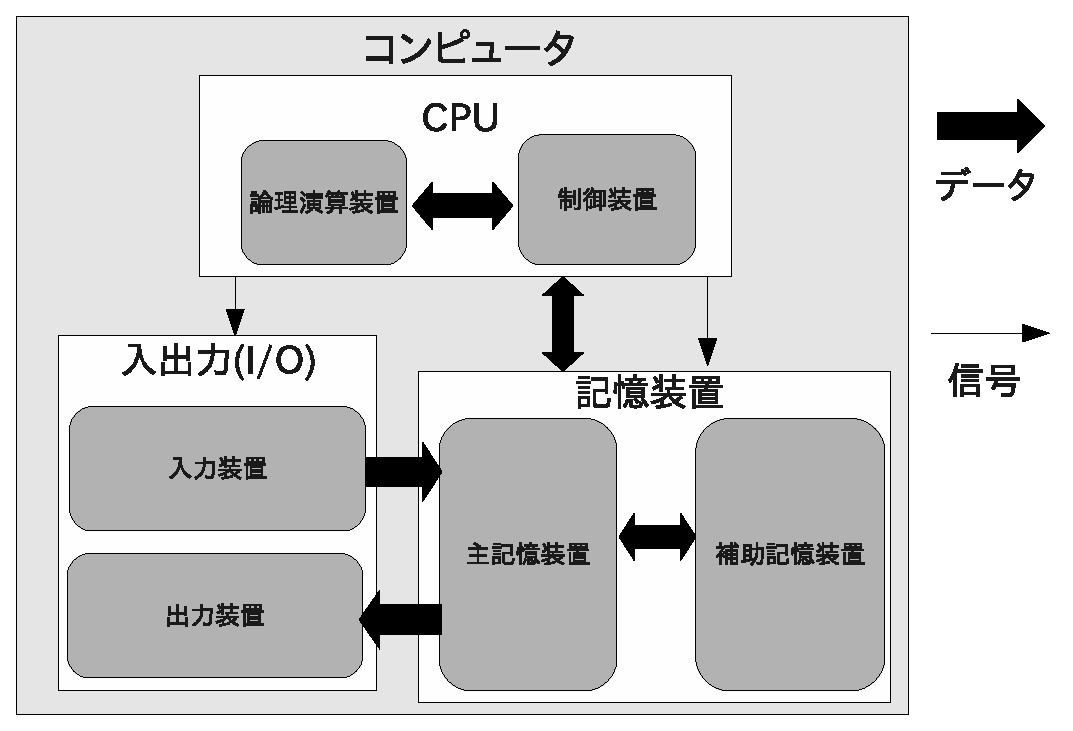
\includegraphics[width=0.9\linewidth,keepaspectratio]{fig0_1.eps}
\caption{コンピュータの装置間の動作}\label{fig0_1}
\end{figure}

\subsection{主記憶装置}
今後学んでいくC言語では、メモリをはじめとした主記憶装置について意識しないといけない場面が数多く出てくる。この為、主記憶装置については他の装置以上に深い理解が要求される。C言語そのものを学ぶ前に、主記憶装置への理解を深めておこう。
\minisec{主記憶装置の種類}
主記憶装置は、CPUからの距離に応じて大別される。

CPUはその最も近いところに\textbf{レジスタ}\index{れじすた@レジスタ}(register)と呼ばれる主記憶装置を持っており、これが一番高速に用いられる主記憶装置である。次いで、\textbf{キャッシュメモリ}\index{きゃっしゅめもり@キャッシュメモリ}(cache memory)と呼ばれる主記憶装置がある\footnote{さらに、キャッシュメモリ自体も近い順に1次、2次、3次と大別される}。そして、我々が一般に\textbf{メモリ}\index{めもり@メモリ}(memory)と呼んでいる主記憶装置(実際に区別するためには\textbf{メインメモリ}と呼ぶことが多い)があり、この3つによって主記憶装置が成り立っている。

このように3つに分けているのは、CPUから近ければ近いほど高速であるが、その分容量が減るためである。例えば、レジスタはメモリに比べるとずっと小さい。従って、必要に応じて、「どの主記憶装置を用いるべきか」も考慮しなければならない。

\minisec{RAM}
メインメモリは\textbf{RAM}\index{RAM}(Random Access Memory)とも呼ばれる\footnote{似た言葉に\textbf{ROM}\index{ROM}があるが、これはRead-Only Memoryの略で、一度書き込んだら書き換えられないような領域を指す。}。これは、前から順に「どこに書きこめばよいか」を探さなければならない\textbf{シーケンシャルアクセス}\index{しーけんしゃるあくせす@シーケンシャルアクセス}(sequential access)を用いると、メモリへのアクセス速度を損ねてしまうからである\footnote{なお、HDDは比較的シーケンシャルアクセスに近いアクセスで、目的のファイルを読み出すのに時間がかかる。一方、SSDはランダムアクセスの性能が高く、HDDより高速なアクセスを実現している。}。どこか空いているところを電気的にすぐに判定し、そこに書きこむようにする\textbf{ランダムアクセス}\index{らんだむあくせす@ランダムアクセス}を用いて速度を損ねることなく利用できるようにしているのである。

また、ランダムアクセスすると、メモリ全体の使われる頻度が均一になり、長持ちしやすいという利点もある。
\\ \\ 
メインメモリには、ここに述べたようにランダムアクセス方式を用いる。このため、RAMと呼んだ場合はメインメモリのことを指すのが一般的である。

\minisec{メモリの領域}
C言語を用いてプログラミングを行う場合、メモリの領域は次の4つに大別される。
\begin{itembox}[l]{Cにおけるメモリ領域}
\begin{itemize}
\item \textbf{プログラム領域}\index{ぷろぐらむりょういき@プログラム領域}:プログラムを実行するためのプログラムコードが置かれる領域。プログラムを実行したい場合、そのプログラムはメモリ上にロードされ、順次実行されることになる。このロードに使われる領域の事。
\item \textbf{静的領域}\index{せいてきりょういき@静的領域}:外部変数や静的変数といった、プログラムの実行中に変化しない(実行中ずっと寿命が保たれている)変数を格納する領域。寿命については後に学ぶ。
\item \textbf{スタック領域}\index{すたっくりょういき@スタック領域}:一般の変数、関数の引数や返却値、長い計算式の一時変数などが置かれる領域。
\item \textbf{ヒープ領域}\index{ひーぷりょういき@ヒープ領域}:プログラム中で動的にメモリが確保される場合に使われる領域。
\end{itemize}
\end{itembox}

自作のプログラムを実行したとしよう。実行されたプログラムは、まずプログラム領域にロードされる。この時、静的領域とスタック領域が割り当てられる。これらの大きさはプログラム実行中不変であるが、静的領域は領域内の使用量が実行中に変化しないのに対し、スタック領域では領域内の使用量が実行中に変化する。このことから、スタック領域の割り当ては「スタック領域をどれだけ使っていいか」という、限度の割り当てである。

以上でプログラムがロードされたら、このあとはプログラム領域の命令を順次読み取ってCPUが処理を実行する。この際、プログラム側が動的にメモリを確保したいと要求すればヒープ領域を用いることになる。

現状ではまだピンと来ない説明かもしれないが、本書を学んでいくうちに、必要に応じてここに戻ってきていただければ、理解できるだろう。

\minisec{メモリとアドレス}
メモリはランダムアクセスであるが、その場所がわからないと困る。そこで、メモリには\textbf{アドレス}\index{あどれす@アドレス}(address)という番号がふられており、これによってメモリ上に配置されているデータの場所が示される。

プログラミング言語を機械に近づけていくと、このアドレスを用いたメモリいじりが主体であることがわかる。逆に、近年生まれた「人間に近い」言語はアドレスいじりを直接目に見える形では行わない場合が多い。

ひとまずここでは、メモリの番地を表すアドレスという指標があるという事を知っておいていただきたい。

\minisec{スタック領域とヒープ領域の特徴}
先に説明したスタック領域とヒープ領域の特徴について、少し記しておく。
\\ \\ 
まず、ヒープ領域はある種の共通領域で、割り当てなどがないのに対し、スタック領域には割り当てがあるという点が違う。メモリが空いている時、ヒープ領域は空いている限り使うことができるが、スタック領域はいくらメモリが空いていても割り当てられた量までしか使うことができない。この為、スタック領域を使い過ぎると、\textbf{スタックオーバーフロー}\index{すたっくおーばーふろー@スタックオーバーフロー}(stack overflow)、日本語に訳すと「スタック溢れ」が起こり、プログラムが強制終了されてしまう。なお、スタックオーバーフローは、メモリ上のアクセス禁止領域にアクセスした事を意味する\textbf{セグメンテーション違反}\index{せぐめんてーしょんいはん@セグメンテーション違反}(segmentation fault)として検出される場合もある。

一方で、ヒープ領域はそう簡単には一杯にならないが、プログラマがその利用を指示しなければならない他、後始末(使用後にメモリを解放する)など必要な処理が自動化されていない(C言語の場合)などの欠点がある。また、ヒープ領域がいくら多いといえど有限であるので、一杯になってしまう場合もある。悪いことに、ヒープ領域が一杯になっても検知されないことがあり、パソコンの動作が不安定になったり、問題が起こったとしてパソコン自体が強制シャットダウンされてしまったりする場合もある。
\\ \\ 
また、スタック領域はメモリのアドレスの大きい方から小さい方に向かって、ヒープ領域はメモリのアドレスの小さい方から大きい方に向かって使われるという特徴がある事を付記しておく。

\subsection{ソフトウェアの分類}
以下、ソフトウェアの分類について簡単に説明しておく。
\minisec{基本ソフトウェアと応用ソフトウェア}
ソフトウェアは大きく分けて\textbf{基本ソフトウェア}\index{きほんそふとうぇあ@基本ソフトウェア|see{OS}}と\textbf{応用ソフトウェア}\index{おうようそふとうぇあ@応用ソフトウェア}に分かれる。
\\ \\ 
基本ソフトウェアは\textbf{オペレーティングシステム}\index{おぺれーてぃんぐしすてむ@オペレーティングシステム|see{OS}}(Operating System,\textbf{OS}\index{OS})とも呼ばれ、基本的なシステムを司るソフトウェアである。つまり、キーボード入力や画面出力といった入出力機能やディスクやメモリの管理など、多くのアプリケーションソフトから共通して利用される基本的な機能を提供し、コンピュータシステム全体を管理する役目を持つ。Windowsをはじめ、Mac,Google Chrome OSや後述するLinux、スマートフォン向けのGoogle Android,Firefox OSなどがOSの具体例である。
\\ \\ 
応用ソフトウェアは文書の作成、数値計算など、ある特定の目的のために設計されたソフトウェアのことを指す。これらのソフトは、OSがまとめている基本的な機能を応用する形で、ユーザに必要な機能を提供する。
\\ \\ 
本書で学ぶC言語は基本ソフトウェアを作ることも可能な言語である。だが、そのレベルまで達するのはまだ先のことである。ひとまず本書では、Windows/Linux上で動かす応用ソフトウェアを作成することにする。

\minisec{ユーザインターフェイスによる分類}
\textbf{ユーザインターフェイス}(User InterFace,\textbf{UI}\index{UI})とはユーザに対する情報の表示様式やデータ入力方式を規定する、コンピュータシステムの「操作上の見た目」「操作するための装置の配置」「操作する際の感覚」のようなものを意味する言葉である。これは、文字をベースとした\textbf{CUI}\index{CUI}(Character-based User Interface)とマウスなどで視覚的に扱うことができる\textbf{GUI}\index{GUI}(Graphical User Interface)に大別される。これは操作の見た目であるため、ソフトウェアの分類でもある。つまり、コマンドを打って操作を実行するようなCUIソフトと、マウスでクリックするなどして操作を行うGUIソフトがある。

本書では初心者向けという観点から、作成の簡単なCUIのみを対象として説明する。GUIはCUIよりも複雑になりがちなためである。

\section{Cプログラミング環境構築}
ここでは、本書で学ぶC言語プログラミングの学習環境を構築するための方法を説明する。なお、本書ではLinux Mint+emacs+gccという環境を元に記しているが、必ずしもこれに従う必要はない。
\subsection{Windowsでの環境構築}
Windowsについては、「苦しんで覚えるC言語」というサイトの管理人であるMMgames氏が学習用C言語開発環境というものを公開しており\footnote{\url{http://9cguide.appspot.com/p_9cide.html}}、これをインストールするだけで学習環境が手に入る。Windowsでの本書の学習については、この環境を利用すれば良いだろう。

あるいは、Web上のサービスにも"ideone"等C言語の開発環境を提供してくれるものがあるので、こちらを利用しても良いだろう(詳しくは付録Cを参照)。

\subsection{Linuxについて}
先に書いたとおり、本書ではLinux MintというOSを元にして記している。これはLinuxというOSの一種である。

Linuxは主として開発者に使われることが多いOSで、オープンソースのOSである。LinuxはUNIXというOSを真似し、これに様々な拡張機能を付加したものであり、これらは共にC言語で書かれている。C言語を学んだ後、これらのソースを読めば文法的に読めないことはないはずである(処理などは難しいが)。なお、Linuxは様々なOSのベースとなっており、モバイル向けのOSなどの中にもLinuxを元としたものが見られる。
\\ \\ 
Linuxはその用途に応じて様々な配布形式(\textbf{ディストリビューション})があり、用途に応じて選択することができる。筆者の環境はLinux Mintというディストリビューションのバージョン13であり、デスクトップ向けのLinuxディストリビューションである。ディストリビューションは他にも多くの種類があり\footnote{例えば、筆者が試したことのあるLinuxディストリビューションはLinux Mintの他、Ubuntu, Vine, CentOS, Scientific, Fedora, RHEL, Mageia, Momonga, Sabayon, Calculate, SolusOS, Stella, arch, puppy, windos, pear, knoppix, KUbuntu, LUbuntu, openSUSE, snow, ultimate edition, zorin OS等多岐に渡る。}、DistroWatch\footnote{\url{http://distrowatch.com/}}やDistroFreak\footnote{\url{http://www.distrofreak.com/}}といった、ディストリビューション情報を専門としたサイトも見られる。ディストリビューションの選択については自分で情報を集めてもらってもよいが、初心者向けにすすめるならばLinux Mint, Ubuntu, Vine辺りが使いやすく情報も多いだろう。

なお、本書は原則Linuxのディストリビューションとは独立して解説を行うが、この講についてはLinux Mint 13を元に記す(Linux Mint 13でなければいけないというわけではない)。

\subsection{Windowsホスト環境へのLinuxの導入}
Windowsが元々入っている環境にLinuxを入れるには、次のような方法がある。
\begin{itembox}[l]{Windowsホスト環境にLinuxを導入する方法}
\begin{itemize}
\item 仮想マシンを用いる。VMwareやVirtual Boxが有名である。
\item 簡易インストーラーが付いているLinux(Ubuntu(Wubi)やLinux Mint(Mint4win)など)を用いてインストールする。
\item HDDの領域(パーティション)を分けて、分けた部分の領域にLinuxをインストールする。
\end{itemize}
\end{itembox}

この内、仮想マシン以外の方法は起動時にどのOSかを選ぶ\textbf{マルチブート}\index{まるちぶーと@マルチブート}(multi boot)になり、両方のOSを同時に使うことはできない。一方、仮想マシンを用いれば2つのOSを同時に使うことができるようになるが、マシンパワーがなければ動作が重くなる。

Linuxのインストール方法はディストリビューションやバージョンによって様々に変わるため、ここでは記さない。ディストリビューションとインストール方法を決めたら「Linux mint インストール」などとしてインターネットを検索し、適切な情報を探しだしてインストールしていただきたい。

\subsection{Linuxの端末操作}
Linuxをインストールしたら「端末」を探して開いてみよう。端末はLinuxのCUI環境をGUI上で再現するソフトで、標準で用意されているものの他、機能をつけた様々な端末も出回っている\footnote{例えば筆者はGuakeという名前の端末を使っている。}。

端末ではコマンドと呼ばれる様々な命令を打つことで、様々の処理を行うことができる。以下、これについて見ていこう。

\minisec{パス}
端末操作をする前に、端末操作に必要な「場所」の概念について説明をしておく。
\\ \\ 
端末を起動した場合、ユーザーのホームディレクトリと呼ばれるディレクトリ(=フォルダ)から始まるのが基本である。これが「現在見ているディレクトリ」(\textbf{カレントディレクトリ}\index{かれんとでぃれくとり@カレントディレクトリ})である。一般に、ホームディレクトリは\verb|~|と、カレントディレクトリは\verb|.|と、カレントディレクトリの一つ上の階層のディレクトリは\verb|..|と表される。
\\ \\ 
ディレクトリやファイルの場所を示す、いわばファイルの住所を\textbf{パス}\index{ぱす@パス}(path)と呼ぶ。パスには、現在いる位置を起点として記す\textbf{相対パス}\index{そうたいぱす@相対パス}と、すべてのディレクトリの根本に当たる\verb|/|からその場所を示す\textbf{絶対パス}がある。例えば、\verb|./Document|などと記せば、カレントディレクトリの下のDocumentというファイルを示すし、\verb|/home/user/Document|のように記せば、\verb|/home|というディレクトリの下の\verb|user|というディレクトリの更に下にあるDocumentというファイルを示す。Linuxの場合、パスの区切りは\verb|/|によって行われる。

\minisec{端末のコマンド操作の例}
端末には多くのコマンドがある。ここでは、プログラミングに必要なコマンド操作を体験してみよう。
\\ \\ 
まず、カレントディレクトリを調べることにしよう。この時には
\begin{code}
pwd
\end{code}
というコマンドを実行すれば良い。その後、
\begin{code}
ls
\end{code}
というコマンドを実行すれば、カレントディレクトリの中身を見ることができる。より詳細に見たい場合には
\begin{code}
ls -al
\end{code}
と\verb|-al|オプション\footnote{オプションとは、実行するコマンドに条件等を付す機能で、通常\verb|-|や\verb|--|等の後に決まった文字(列)を記して指定する。}をつければ良い。
\\ \\ 
この下に\verb|test|ディレクトリを作ってみよう。ディレクトリの作成には
\begin{code}
mkdir ディレクトリ名
\end{code}
というコマンドを用いる。この場合は
\begin{code}
mkdir test
\end{code}
とすれば、カレントディレクトリの下にtestというディレクトリが作られる。
\\ \\ 
次いで、今作ったディレクトリの中に移動しよう。フォルダを移動するには
\begin{code}
cd 移動先フォルダのパス
\end{code}
というコマンドを実行する。従って、ここでは
\begin{code}
cd ./test
\end{code}
のように打てば良い。この際、パスをいちいちすべて打つのは大変なので、tabキーを押しながら打つことをすすめる(特段なければ、\verb|./t|まで打った後にtabを押すと良いはずである。)。tabキーは入力を補完してくれる機能で、コマンド、パスを含め端末の様々な場面で使うことができる。
\\ \\ 
ここに、空のファイル\verb|empty|を作成してみよう。これには
\begin{code}
touch ファイル名
\end{code}
とすれば良い。
\\ \\ 
更に、このファイルをコピーして、\verb|empty2|というファイルを作成してみよう。ファイルのコピーは
\begin{code}
cp コピー元ファイル名(パス) コピー先ファイル名(パス)
\end{code}
とすれば良い。
\\ \\ 
次は、\verb|empty|をリネームして\verb|empty3|にしてみる。リネーム及びファイルの移動は
\begin{code}
mv ファイルの移動(リネーム)元 ファイルの移動(リネーム先)
\end{code}
と記す。
\\ \\ 
最後に今作ったファイルとディレクトリを削除してみよう。ファイルの削除には
\begin{code}
rm 削除したいファイル名
\end{code}
を用いる。ここでは\verb|empty2|と\verb|empty3|を削除しよう。これを1行ずつ実行しても良いのだが、面倒であるので、
\begin{code}
rm empty?
\end{code}
というコマンドを実行してみると良い。これにより両ファイルが消えるはずである。ここで用いた\verb|?|は後に示すワイルドカード表現と呼ばれる表現である。
\\ \\ 
ディレクトリを消すため、まず、一つ上のディレクトリに移る。これは
\begin{code}
cd ..
\end{code}
を実行すれば良い。最後に
\begin{code}
rmdir 削除したいディレクトリ名
\end{code}
とすれば、ディレクトリが消える。
\\ \\ 
なお、コマンドを調べるためには
\begin{code}
man コマンド名
\end{code}
と記せば良く、これによってコマンドのマニュアルを見ることができる。また、多くのコマンドは\verb|--help|オプションを付して実行することで簡易ヘルプを表示してくれる。

ここで、プログラミングに使うコマンドはひと通り体験したつもりであるが、これ以外のコマンドで知りたいものがあればmanコマンドなどを利用して調べて欲しい。なお、Linuxのコマンド一覧はインターネットで探せば多く見つかる\footnote{例えば、\url{http://itpro.nikkeibp.co.jp/article/COLUMN/20060224/230573/}など。}。

\minisec{ワイルドカード表現}
先に使った\verb|?|は\textbf{ワイルドカード表現}\index{わいるどかーどひょうげん@ワイルドカード表現}と呼ばれる表現であり、\verb|?|以外にもうひとつ\verb|*|という記号を用いる場合もある。これは、似たような名前のファイルに対して同じ操作をする場合などに、まとめて行うことができる手法である。

\verb|?|のワイルドカードは、1文字の任意文字を示す。例えば、\verb|empty?|と先に書いた例は、\verb|emptyl|や\verb|empty9|など、\verb|empty|の後に1文字を付した形のファイル、という意味になる。

\verb|*|のワイルドカードは、0文字以上の任意文字列を示す。例えば、\verb|*.txt|と書いた場合、\verb|code.txt|や\verb|temp.txt|など、最後が\verb|.txt|で終わる全てのファイル/ディレクトリを示している。

\minisec{リダイレクト}
コマンドを実行した場合、その結果はコマンドラインに出力される。また、実行されたコマンドによっては、更に入力を要求される場合もある。この入出力先を変更する方法として\textbf{リダイレクト}\index{りだいれくと@リダイレクト}(redirect)がある。
\begin{itembox}[l]{リダイレクト}
リダイレクトを行う場合には、コマンドに続けて
\begin{code}
>出力先ファイル名
\end{code}
や、
\begin{code}
<入力元ファイル名
\end{code}
を記す。これらを両方共用いることもできる。
\end{itembox}

試しに、
\begin{code}
ls -al > ls_list.txt
\end{code}
というコマンドを実行してみると、\verb|ls_list.txt|というファイルに\verb|ls -al|コマンドの実行結果が出力されているはずである(moreコマンドやlessコマンドで確認してみよ)。
\\ \\ 
作成したCUIソフトのテスト時などに、これらのリダイレクト入出力が役立つ。

\subsection{Linuxでの環境構築}
最後に、LinuxでのC言語の環境構築方法を述べておく。

まず、
\begin{code}
which gcc
\end{code}
により、gccというコマンド(ソフト)がインストールされているかどうか確認する。このコマンドを実行して、もしもパスが表示されなかったならば、後でテキストエディタをインストールする際にgccを同時にインストールする必要がある。gccはコンパイラというソフト\footnote{gccの他、IntelやAMD,Microsoft,Embarcaderoなどからもコンパイラが出ている。}で、簡単に言うとC言語で書いたプログラムのソースから実行ファイルを生成するためのソフトである。
\\ \\ 
次いで、自分の好みのテキストエディタをインストールする\footnote{インターネットに接続する必要がある。}。以下ではemacsを例にとるが、gedit, tea, leafpad, editra, vimなど、好きなテキストエディタを用いれば良い(その際は、emacsを他のテキストエディタ名に読みかえること)。

ソフトをインストールする場合、Linux MintやUbuntuならば
\begin{code}
sudo apt-get install ソフト名
\end{code}
を実行し、その後にユーザーパスワードを入れれば良い。

Vineの場合は
\begin{code}
su
\end{code}
コマンドを用いて(管理者のパスワードを打ち込み)管理者モードになった後
\begin{code}
apt-get install ソフト名
\end{code}
によりインストールを行う。

この他、ディストリビューションによっては、\verb|apt-get|の部分が\verb|yum|等、別のコマンドに変わる場合がある。
\\ \\ 
上記より、Linux Mintにgccとemacsを導入する場合は
\begin{code}
sudo apt-get install gcc emacs
\end{code}
というコマンドを実行すれば良い。
\\ \\ 
emacsをインストールしたら、端末を再起動した後、
\begin{code}
emacs ファイル名
\end{code}
を実行すれば、emacsが立ち上がり、引数で指定したファイルを編集できる。
\newpage

\begin{shadebox}
\section*{本講の要点}
本講ではプログラミングを行うための知識・環境の準備を行った。以下、知識のみまとめておく。
\subsection*{記数法}
\begin{itemize}
\item $n$進法とは、$n$を位取りに用い、$n^k$を各位とする記数法である。
\item $n$進法から10進法に変換する場合には、単に各位の数とその位の元となる$n^k$の積の総和を取れば良い。
\item 10進法から$n$進法に変換する際には、順次$n$で割って剰余を列挙し、この剰余を逆から順に記せば良い。
\item 8/16進法は2進法と相互に直接変換することができるため、コンピュータでよく用いられる。
\item 2進法1桁の事を1bitと呼び、8bitのことを1octetと呼ぶ。
\item 通常のコンピュータでは、1octetのことを1Byteと呼び、データの単位に用いている。
\end{itemize}

\subsection*{コンピュータの仕組み}
\begin{itemize}
\item パソコンは入力装置・出力装置・CPU・記憶装置からなる。
\item 主記憶装置は、CPUからの「近さ」に応じて、レジスタ、キャッシュ、メモリなどとわけられる。
\item メモリへのアクセスは通常ランダムアクセスである。
\item メモリはプログラム領域・静的領域・スタック領域・ヒープ領域にわけられる。
\item メモリ上での位置は、アドレスを用いて示される。
\item スタック領域はアドレスが大きい側から小さい側へ向かって取られ、プログラム毎に使用限度が定められる。一方ヒープ領域は、アドレスが小さい側から大きい側へ向かって取られ、空いている限り使うことができる。
\item ソフトウェアはその機能から、OSと応用ソフトウェアに分かれる。
\item ソフトウェアのUIは、GUIとCUIとに分かれる。
\end{itemize}
\end{shadebox}


\chapter{プログラミングとは何か}
それでは、プログラミングについて学んでいこう。ここではまず、プログラミングとは何かという概論を話す。次いで、どのようにして作るのかという基本的な手順を学んだ後、標準出力への出力という、最も単純なプログラムを組んでみる。
\section{プログラミングとは何か}
「\textbf{プログラミング}\index{ぷろぐらみんぐ@プログラミング}(programming)とは何か」というタイトルはこれからプログラミングを学ぼうという人にとって大変親切で、かつ適切なタイトルであるが、同時に様々な意味をもち、ある程度プログラムに慣れた人にとってもある種の意味をなす質問だろう。プログラミングとは何か、その質問に対して、もちろん、一般的に辞書的に意味を説明するのが本講の目的だが、その質問は辞書的以外の意味をも十分持ちうるのである。例えば「私にとってプログラミングとは何か」という、人の思いに対する質問とも捉えられるし、「社会的にプログラミングとはどういった価値をもつのか」という、位置づけを問うこともできる。ある種のジョークのように聞こえるかもしれないが、哲学的に「プログラミングとは一体何なのか?」と考察することもできよう\footnote{ここではジョークのように聞こえると書いたが、決してプログラミングと哲学が無関係なわけではない。例えばPrologという言語はAI(人工知能)の研究によく用いられるプログラミング言語であるが、AIの根幹の部分ではルートヴィヒ・ウィトゲンシュタインの「論理哲学論考」などが大きな役割を果たしている。哲学に不案内であっても、「AIというものがあるとき、それをそもそも作ったプログラミング言語というのは一体何か?」という問いかけは、「人間の知能のプログラミング言語にあたるものは存在するのか?」という哲学的に思える問いに直結することがわかるだろう。}。ともかく、「プログラミングとは何か?」という問いはその文脈によって大きく変わりうるものである。そして、読者諸賢には、本書の内容を身につけていただくにしたがって「私にとってプログラミングとは一体何か?」ということも考えていただきたい。
\\ \\ 
さて、プログラミングとは一体何なのか、辞書的にみていくこととしよう。手持ちの「新明解国語辞典(三省堂)」を引くと、次のように書かれている。
\begin{itemize}
\item プログラミング:コンピュータにさせる仕事の手順を詳しく分析し、プログラムを作ること。
\item プログラム:コンピュータに実行させる計算処理の手順を、コンピュータに受け入れ可能な一連の命令文の形で並べて書いたもの(あるいは書くこと)。
\end{itemize}

一方、Wikipediaには次のように書かれている。
\begin{itemize}
\item プログラミング:プログラムを作成することにより人間の意図した処理を行うようにコンピュータに指示を与える行為である。
\item プログラム:コンピュータに対する命令処理を記述したもの。
\end{itemize}
見比べればわかる通り、どちらも大差ない説明である。そして、どちらも間違っていないが、どうも無味乾燥であり、いかにも難しいといったもののように思えてしまう。
\\ \\ 
プログラミングを好んでいる人がいて、それを趣味としている筆者のような人もいるほどなのだから、こんなにも冷たい説明では実感がわきにくい。辞書の説明だから冷たいのは当然であるが、もう少し具体的に、躍動感のある意味を追求してみよう。我々が日常的に目にするドラマ・映画などはお芝居であり、脚本がある。芝居のときに人間がどのように動けばいいかを記したのが脚本であるのと同様に、何かをなすとき、例えばゲームを動かすときに、コンピュータがどのように動けばいいかを記したものがソースコードというプログラムの"もと"である。マニュアルの作成と言ってもいいが、手順書を作成し、コンピュータを動かすことで何かをなす、それがプログラミングである。その何かはゲームでもいいし、音楽でもかまわない。あるいは文書処理や翻訳かもしれない。ともかく、そういった行為を行う際に動く手順を定め記すのがプログラミングである。それは脚本を書くように創作的な行為であり、でき上がりのドラマを見る楽しみをコンピュータ上で味わえるものである。プログラマーは脚本家と監督を兼任し、コンピュータが俳優の役割をする。そうしてでき上がったドラマをプログラムと呼んでいる。このように記せば、プログラミングが生きたものとして伝わってくるのではないだろうか。

\section{プログラミング言語とC言語}
先に記したとおり、プログラミングとはコンピュータがどのように動けばいいかを記す行為である。何かを記すには、言葉が必要である。プログラミングを行うための言語を\textbf{プログラミング言語}\index{ぷろぐらみんぐげんご@プログラミング言語}(programming language)という。プログラミング言語は多種多様であり、各言語はそれぞれに特徴を持っている。そのため、一般には利用目的に適したプログラミング言語を選ぶ。

プログラミング言語にはいくつもの分類があるが、ここでは、Cのソースコードを書いてそれが実行されるまでの流れを理解するのに重要な「高級言語」「低級言語」を紹介する。
\subsection{高級言語・低級言語と処理の流れ}
通常、プログラムは1と0からなる機械語およびそれをもう少しまとめたバイトコードとしてメモリにロードされ、それが実行される。これは、コンピュータが唯一理解、実行できる形態である。プログラミングとは、この1と0を適当な順番に配置し、希望する機能を実現することである。だが、直接1と0を配置するのは問題がある。というのは、CPUに応じて命令セットが違うためである。また、この形式では当然、人間にはわかりにくい。そこで、これらの汎用性を高め、人間にわかりやすいようにした。このようにして生まれた、人間にわかりやすく、CPUの命令セットによらずにプログラミングできる言語のことを\textbf{高級言語・高水準言語}\index{こうきゅうげんご@高級言語}\index{こうすいじゅんげんご@高水準言語|see{高級言語}}と呼ぶ。

高級言語で書かれたソースは、各々のCPUにおいて、その機械語と1対1に対応する命令によって書かれたバイトコードに変換される。このように、機械語及びそれと1対1対応する、機械毎に固有の言語(命令セット)を\textbf{低級言語・低水準言語}\index{ていきゅうげんご@低級言語}\index{ていすいじゅんげんご@低水準言語|see{低級言語}}と呼ぶ。また、この変換(翻訳)行為を\textbf{コンパイル}\index{こんぱいる@コンパイル}(compile)と呼ぶ。我々は高級言語、ここではそのひとつであるC言語を用いてプログラムを記述し、そのソースをコンパイル、低級言語で書かれたバイトコード(実行ファイル)を生成して、プログラムを実行するのである。

\subsection{C言語の特徴}
C言語は高級言語であるが、その特徴から俗に「高級言語の顔をした低水準言語」や「中級言語」などと呼ばれることもある。その特徴には、次のようなものがある。
\begin{itembox}[l]{C言語の特徴}
\begin{itemize}
\item C言語は、構造化手続き言語\footnote{構造化手続き言語とは、E.W.Dijkstra(1930-2002)の提唱した「\textbf{構造化プログラミング}\index{こうぞうかぷろぐらみんぐ@構造化プログラミング}:あらゆるアルゴリズムは連接(順次)・分岐・反復の3構造により実現でき(\textbf{構造化定理}\index{こうぞうかていり@構造化定理})、その3構造を関数などによって適度に分離、ルーチン毎に細部を記述していくというプログラミングパラダイム」に従い、手続きを順に記すことでプログラムを作成する言語である。}である。
\item メモリのレベルまで含めた、かなり機械に近い処理ができる。
\item システム記述に向いている言語である。
\item プログラミング人口が多い。Tiobe programming community\footnote{\url{http://www.tiobe.com/index.php/content/paperinfo/tpci/index.html}}によれば、2002年以後世界で1〜2位のシェアを誇る。
\item 非常に自由度が高く、大抵の機能を実装することができる。これは、悪く言えば、コンピュータにとって危険な処理も作れてしまうということである。
\item 基本的にプログラマに信頼を寄せた言語となっており、自動的に行われる処理は少ない\footnote{逆に、Javaは危険な処理を自動的に検知し、些か口煩いと思う人もいるぐらいに忠告をする言語である。}。これは、自由度が高いがゆえにプログラマに重責があるということでもある。
\item 様々な言語の基になっている。
\end{itemize}
\end{itembox}

とりわけ、自由度が高く、低水準命令が可能でシステム記述に向いていることから、UNIXを始めとしたOSカーネルや組み込みプログラミング\footnote{家電等「いわゆるコンピュータ」ではない様々な機器のシステム等のプログラミング。}に利用されている。

\subsection{C言語の歴史}
C言語は現在一般に使われているプログラミング言語ではかなり古い部類に入る言語である。C++やJavaなどの言語がCの構文を元にしていることからもわかるとおり、非常に多くの分野で使われている言語であるが、この言語にも元の言語が存在する。それがBCPLとBである。前者はオペレーティングシステムやコンパイラを書くために開発された言語で、これをモデルにしてUNIXオペレーティングシステムの初期バージョン開発に向けて作られたのがBであった。1960年後半〜70年代にかけてのことである。
\\ \\ 
アメリカ・ベル研究所のD.M.Ritchie(1941-2011)はBを元にしてC言語を作った。これがC言語のはじめである。この時代においてのC言語は、小型で効率的であり、しかも強力なプログラミング言語であったため(現代でも強力と言い切れるかどうかは、特にC++と比べてそう言えるかどうかは、疑問の余地が残るが)、多く使われるようになっていった。だが、この広まり方はC言語の“方言”とでも言うべき、様々な「規格」を生み出す要因となってしまった。この是正のため、1982年、ANSI(American National Standards Institute)内で委員会が組織され、その時点で最も広まっていたCの方言である「K\&R C」\footnote{B.W.Kernighan(1942-)と(先に名の出てきた)RitchieのCという意味である。この二人は「プログラミング言語C(The programming language C)」というCの原点とも言うべき書籍を著した。惜しいことに、Ritchieは2011年10月に亡くなってしまったが、Kernighanは存命である。「プログラミング言語C」はANSI規格(C89)に対応した第2版が出版されており、通称「K\&R本」として広く知られている。なお、日本語版は石田晴久氏の訳が共立出版より出版されている。}を基に標準規格を定める運びとなった。委員会発足から7年を経た1989年、規格化されたC言語、現在に至るまでANSI C(C89)と呼ばれるC言語が誕生したのである。現在のコンパイラは少なくともこの規格に則っているものとして問題ないし、また、この規格より以前のC文法に従ってコードを書く意味はないと言って良い。この規格がそのまま国際標準となり、現在のCの基盤をなしているからである。
\\ \\ 
だが、1989年の規格に一切の改良が行われなかったわけではない。とりわけ、1999年のC++を意識した規格の変更は大きなものであった。本書を書いている2012年現在、1995年と1999年、2011年に、C言語は三度の改訂を経ている。1995年の改訂は89年制定のCに対して、各国の文字を扱えるようにする改訂であった。これは、それまでのCに対して軽い追加が行われた程度のものであり、大きな変動ではなかった。

一方、1999年制定のCはC99とも呼ばれるかなり大幅な拡張であった。89年のCに対して、C++を意識した拡張を行ったのがこの改訂である。1989年以降のCで書かれたコードであれば、大抵は現在のこのC99規格でも動くと考えて差し支えない。だが、この規格は意外と知られておらず、書店に並んでいる本を見ても、この事まで書いている本は多くなく、むしろごく一部にC99の概念が取り入れられている程度に過ぎない本が多い。特によく目にするのが、\verb|//|によるコメントを説明していながら(このコメントはC99規格で取り入れられたもので、C89の規格では通用しない。コメントについてはあとのページを参照されたい。)、これがあたかも昔からのCに存在するかのように書いている本である。明確にされていないが、背景でC99を使っているのである。
\\ \\ 
2011年にC++11というC++の新規格と共に出されたCの新規格はC11と呼ばれている。ここでの改訂は、C言語をより現代的な視点に対応させるための改訂と言える。しかしながら、この規格は、出てから時間が経過していないという事もあり、対応しているコンパイラが少ない。また、本書の段階でC11で新たにできた文法が必要になることは少ない。このことを踏まえ、本書ではC99の規格を基に、旧来のC規格にも通用する内容を記述することにする。C11については脚注などで触れるに留める。

\section{プログラム作成の一連の流れ}
プログラムの作成は概ね、次の順で行われる。
\begin{enumerate}
\item 作成したいものを決める。(プログラムの計画)
\item 作成したいものをどのようにしてプログラムにするかを決める(\textbf{アルゴリズム}(algorithm)\index{あるごりずむ@アルゴリズム}を立てる)。
\item 立てたアルゴリズムにしたがってソースコードを打つ(\textbf{コーディング}(coding)\index{こーでぃんぐ@コーディング})。
\item 作成したソースコードをコンパイルして実行する。
\item コンパイル中ないしプログラムの実行中にエラーが出た場合は、そのエラーを取り除く(\textbf{デバッグ}(debug)\index{でばっぐ@デバッグ})。
\item ソースコードの無駄な部分を取り除く(プログラムの改良)。
\end{enumerate}
これを実際に体験してみよう。

\subsection{コーディングまでの体験}
はじめなので、あまり難しいプログラムを書くことはできない。今回は最も単純に、標準出力に
\begin{code}
hello, world
\end{code}
と出力するプログラムを作成してみよう。なお、第0講で記したとおり、以降のプログラムは(特段の記述がなければ)Linuxにgccをインストールしていることを前提に行う。
\\ \\ 
まず、端末を開き、適当なフォルダを作成し、そこに移動する。例えば、
\begin{code}
mkdir Clang
cd Clang
mkdir class2
cd class2
\end{code}
とすれば、ホーム以下にClangというフォルダができ、その中にclass2というディレクトリを入れて、そこで作業することになる。
\\ \\ 
フォルダを移動したら、テキストエディタを開こう\footnote{第0講にも記したが、emacsはテキストエディタに応じてtea,editra,gedit等に読み替えること。}。
\begin{code}
emacs Hello.c
\end{code}
 このように書けば、\verb|Hello.c|という名前の\textbf{ソース}(Source code)\index{そーす@ソース}を作ることになる。ここで、ソースというのはプログラムの内容を記述したファイルである。

それでは、次の問題を読んで、書いてある解答例(リスト\ref{program1_1})を打ち込んでみよう。この時、ソースには、適度に空行やタブ(\textbf{インデント}\index{いんでんと@インデント})が入っているが、これはソースを読みやすくするための工夫であるので、その部分も真似してみて欲しい。但し、誤って全角空白を入れないこと(エラーになる)。なお、以降のソースでは、紙面節約のためスペースや空行を省くが、単語等を分割しない範囲で、読みやすいように空白等を入れたほうが良い。
\begin{boxnote}
\minisec{hello worldプログラム}
"hello, world"と出力するプログラムを作成する。
\begin{multicols}{2}
\minisec{解説}
hello, worldと出力するプログラムは、一般に「ハローワールド」と呼ばれており、多くの言語の入門書の最初に挙げられている「世界一有名なプログラム」である。初出は先に記した「プログラミング言語C」であるとされる。\\
 その名の通り、ただhello, worldと出力されるだけのシンプルなプログラムであるが、言語の書式を学ぶ上で、とても重要なプログラムでもある。

\begin{lstlisting}[caption=ハローワールド,label=program1_1]
/* hello, world
   puts Version */

#include<stdio.h>

// main function
int main(void){

  //output for stdout.
  puts("hello, world");

  return 0; //val=0
}
\end{lstlisting}
\end{multicols}
\end{boxnote}

以上を打ち込み終わったら、保存して(emacsの場合、ctrl+xを押した後、ctrl+sを押せば保存できる)、テキストエディタを閉じよう。

\subsection{コンパイル・実行}
さて、それではコンパイルして実行ファイルを生成しよう。コンパイルのコマンドは次の通りである。
\begin{itembox}[l]{プログラムのコンパイル}
あるソースをgccでコンパイルして、実行ファイルを得るためのコマンドは
\begin{code}
gcc (ソースファイル名) -o (出力実行ファイル名)
\end{code}
である。この時、\verb|-o|以下を省略すると、a.outという実行ファイルができる\footnote{Windowsの場合は、a.exeという実行ファイルができる。}。
\end{itembox}

したがって、
\begin{code}
gcc Hello.c -o Hello.out
\end{code}
とすれば、実行ファイルHello.outが生成されるはずである。もし何らかのエラーが出たら、どこかに打ち間違いがあると考えられるので、再度テキストエディタを開いて間違っている場所を調べてみよう。このように、誤り(\textbf{バグ}\index{ばぐ@バグ}(bug)\footnote{原義は「虫」であり、トーマス・エジソンも使っていたことが知られているが、「世界最初のバグ」は昔の大型コンピュータに実際に虫が入ったものであるとされている。})を取り除くことを\textbf{デバッグ}\index{でばっぐ@デバッグ}(debug)と呼ぶ。

続いて、できたファイルを実行する。これは、
\begin{code}
./Hello.out
\end{code}
などとすれば良い。正しくできていれば、コンソール上に
\begin{code}
hello, world
\end{code}
と出力されるはずである。
\\ \\ 
以上のようにして、プログラムを作成することができる。今後、この手続きは何度もやっていくことになるので、今取り立てて覚えずとも、そのうち自然と身につくだろう。

\subsection{「はじめてのプログラム」の解説}
さて、それではリスト\ref{program1_1}のプログラムがどのような動作をしているのか、コードを追いつつ順に説明していこう。

\minisec{コメント}
このプログラムの1,2,6,9行目はコメント行であり、12行目にもコメントがある。\textbf{コメント}\index{こめんと@コメント}(comment)とは、ソースコードのうち、我々人間のために覚え書きとして挿入される注釈のことである。この部分は、コンパイルの際に何も書いていないものと同様に扱われるので、好きなことを書くことができる。この例のようにタイトルを書いたり、文法解説やアルゴリズム解説の際に横に入れたり、デバッグの際に一時的にコードを無効化したりと、色々な用途に使う。なお、本書では紙面節約のため、掲載ソースリストのコメントは省く。だが、一般には別人\footnote{たとえ自分自身しか使わないソースコードでも、コメントを書くに越したことはない。というのは「1か月後の自分は別人と思え」と言われるほど、ソースコードの細部は覚えにくいものだからである。}が読んでもわかるようにコメントを書くべきである。
\\ \\ 
C言語では、コメントは2種類ある。
\begin{itemize}
\item \verb|//|から行末まで。
\item \verb|/*|から始まり、最初に出てくる\verb|*/|まで。
\end{itemize}
前者は1行のコメントまたは命令のすぐ横に使う場合が多い\footnote{実は工夫次第で2行以上のコメントも書けるのだが、わかりにくいので使わないほうが良い。}。このように、行末までをコメントとみなすコメントの形式を\textbf{インラインコメント}\index{いんらいんこめんと@インラインコメント}(in-line comment)と呼ぶ。一方で、後者は、タイトルで使っているように、何かまとまったコメントを書きたい場合に使うことが多い。このように、ある記号から始まりある記号で終わる(この場合、\verb|/*|から始まり\verb|*/|で終わる)コメントの形式を\textbf{ブロックコメント}\index{ぶろっくこめんと@ブロックコメント}(block comment)と呼ぶ。
\\ \\ 
コメントは冗長すぎても良くないし、少なすぎるのも後々困ることになる。コメントの基準は人によるが、概ね処理の要約を基本に、難解な処理に解説をつけていく形でコメントを付すと、読みやすいソースになる。

\minisec{include文}
コメントを抜いて、実質的に意味があるのは4行目である。この行は\textbf{include文}\index{includeぶん@include文}と呼ばれる文で、\verb|< >|で囲まれた\textbf{ヘッダファイル}\index{へっだふぁいる@ヘッダファイル}(header file)を読み込む\footnote{実際にはダブルクォーテーション(")で囲む場合もある。これについては、後の講で説明する。}という意味である。ヘッダファイルというのは、Cの様々な命令(関数)の入っている辞典のような物だと思えば良い。(実際には、辞典そのものは\textbf{ライブラリ}\index{らいぶらり@ライブラリ}(library)と呼び、ヘッダファイルはこれを引くための道具である。)これらの辞典を読み込むことにより、コンパイラは命令を解釈することができる。このことからわかるとおり、この一文はコンパイラへの命令である。このようなコンパイラへの命令のことを\textbf{前処理命令}\index{まえしょりめいれい@前処理命令}または\textbf{プリプロセッサ命令}\index{ぷりぷろせっさめいれい@プリプロセッサ命令}(preprocessor command)と呼び、\#から始める\footnote{この記号(\#)は「シャープ」ではなく「ハッシュ」である。二つの記号は線の角度が違う。}。includeはヘッダファイル等の読み込みを行う前処理命令である。
\\ \\ 
今回読み込んだstdio.hはstandard input and output(標準入出力)のライブラリで、その名前通り、入出力に関する命令が収められているライブラリである。このように、C言語が仕様として標準で用意しているライブラリのことを\textbf{標準ライブラリ}\index{ひょうじゅんらいぶらり@標準ライブラリ}と呼ぶ。
\\ \\ 
以上を踏まえると、リスト\ref{program1_1}の第4行は、「以降で標準入出力の命令を使えるようにするため、stdio.hのライブラリを読み込め」という意味になる。

\minisec{main関数}
プログラムのソースコードは原則上から下に向けて解釈される。だが、実際にはプログラムの主幹を司る部分を各プログラムに一つ作り、その部分を実行することによってプログラムが動く。つまり、プログラムというのは、主部より前に準備のための文があり(先のincludeなどはまさにそれである)、主部があり、その後ろに(必要に応じて)主部を詳述する部分がある、という構成になる。このうち、準備のための文や主部を詳述する部分は必要ない場合もあるが、主部はプログラム毎に必ず1つ必要である。この主部を示すのが\textbf{main関数}\index{mainかんすう@main関数}である(リスト\ref{program1_1}の、第7行から第13行の部分)。当面の間、main関数は次のように記せばよい。
\begin{itembox}[l]{main関数の書き方}
main関数は、次のような形式で記す。(但し、後に学ぶコマンドライン引数を用いる場合はこの限りではない。)
\begin{code}
int main(void){
  処理を記す
}
\end{code}
\end{itembox}
main関数の定義にあるint,voidについては後の自作関数の講で詳しく解説するので、ここでは「このように書くものである」と思っておいて良い。

\minisec{puts関数}
リスト\ref{program1_1}の第10行目は今後Cプログラムを書いていく上で必要なことを多く含む、示唆に富む1行である。動作は"hello, world"と標準出力(コンソール)に出力するだけのものだが、それ以外の、ルールなどの面でこの一文から学べるものは多い。
\\ \\ 
putsはstdio.hに入っている\textbf{関数}\index{かんすう@関数}で、put stringの意味である。この関数は\textbf{引数}\index{ひきすう@引数}(ひきすう,argument)の文字列を標準出力に出力し、\underline{最後に改行する}関数である。ここまでさらりと説明したが、新たな用語が連続しているので、その用語を見ていくこととする。

関数というのは後ろに( )を伴い、何らかの値を与えると、それに対して処理を行い、何かの値を返すものを言う。ここであげたputs関数は、文字列を引数にとり、その引数の文字列を標準出力に出力し(処理)、無事に出力できたかどうかを(内部的に)返す。この時に返す値のことを\textbf{返却値}\index{へんきゃくち@返却値}\footnote{返し値、戻り値などとも言う。「返却値」はJIS規格での呼び方である。}(return value)と呼ぶ。

少しわかりづらいかもしれないので、出前を例に考えてみよう。まず、出前して欲しい店に、電話などで注文を行う。これを受けて、店では注文されたメニューを料理する。その後、店から自分のところに注文した料理が届く。この、注文が引数であり、店での調理が処理、自分のところに届いた料理が返却値である。つまり、出前という関数は「注文」を引数にとって、それに対応した「料理」を返却すると言える。
\\ \\ 
ここまででputsの意味はわかったと思うが、後2点、ダブルクォーテーション(")の意味と、セミコロン(;)の意味について見ていこう。

ダブルクォーテーションは二つセットで、その間が文字列であることを示す\footnote{厳密には文字列リテラルというものであり、これについては後に詳述する。}。

セミコロンは、Cの各文の最後に付ける記号で、日本語の句点(。)や英語のピリオド(.)に相当するものである。

\minisec{return文}
先に書いたとおり、関数は返却値を持つ\footnote{持たない関数もあるが、これは「持たない」ようにしているから持たないのであって、例えば標準ライブラリでは持つ関数のほうが多い。}。そして、main関数は名前が示唆する通り、関数である。したがって、main関数も返却値を持つ(ようにしている)。この返却値を指定するのがreturn文である。

また、関数は返却値が定まった時点で終了するので、関数の終了を示すためにreturn文を用いる場合もある(後述)。

return文で返却値を定める場合は、次のように記す。
\begin{itembox}[l]{return文}
関数の返却値にはreturn文を用い
\begin{code}
return (返却値);
\end{code}
と記すことによって返却値を指定できる。(返却値を持たない関数の終了のみを示す場合、返却値を指定しないこともある(後述)。)
\end{itembox}

main関数は、正常終了した場合0を返すように作る(つまり、return 0を処理の終端に書く)のが慣例である。

\section{標準出力への出力}
簡単なプログラムを一つ作ったところで、もうひとつ、出力するだけのプログラムを作ってみよう。
\begin{boxnote}
\begin{multicols}{2}
\minisec{簡単な表の出力}
簡単な表を出力してみる。
\minisec{解説}
水平タブ文字を用いて場所を揃えることにより、簡単な表を作ることができる。今回は、数学の記号とその正式名称を出力するプログラムを書いてみよう。なお、8行目が2行に渡っているが、実際のプログラムでは1行に続けて書くこと。

\begin{lstlisting}[caption=数学の記号表出力,label=program1_2]
#include<stdio.h>

int main(void){
  printf("Math words.\n");
  putchar('\n');

  puts(" sin \t lim \t sup");
  puts(" sine \t limit \t supremum");
  return 0;
}
\end{lstlisting}
\end{multicols}
\end{boxnote}
\minisec{エスケープシークエンス}
リスト\ref{program1_2}には\verb|\n|や\verb|\t|といった文字が登場する。これらは各々、改行や水平タブを表している。このように、コード上で意味を持っているなどの理由で書き表すことができない文字に対しては、代替となる書き方が用意されている。このような文字のことを\textbf{エスケープシークエンス}\index{えすけーぷしーくえんす@エスケープシークエンス}(escape sequence)とよび、\verb|\|記号\footnote{バックスラッシュ。日本の円マークも同じ役割であり、バックスラッシュが出ない代わりに円マークが用いられる場合もある。}に文字を付けることで実現される。エスケープシークエンスは2文字(以上)に見えるが、実際には\verb|\n|や\verb|\t|で1文字である。よく使うエスケープシークエンスを表\ref{escape_seq}に示す。
\begin{table}[htbp]
 \centering
 \caption{よく使うエスケープシークエンス}\label{escape_seq}
  \begin{tabular}{|c|c||c|c|} \hline
            文字&意味&文字&意味        \\ \hline
              &&&          \\[-15.5pt] \hline
   \verb|\0| & NULL文字 &\verb|\'| & シングルクォーテーション\\ \hline
   \verb|\t| & 水平タブ文字 &\verb|\"| & ダブルクォーテーション\\ \hline
   \verb|\r| & 復帰文字 &\verb|\\| & バックスラッシュ\\ \hline
   \verb|\n| & 改行文字 &\verb|\?| & クエスチョン\\ \hline
  \end{tabular}
\end{table}

表\ref{escape_seq}に載っている\verb|\r|はCR(キャリッジリターン、carriage return)で、Macでの改行コードである。一方\verb|\n|はLF(ラインフィールド、line field)で、Linuxなどでの改行コードである。Windowsの改行コードはCR+LF(\verb|\r\n|)であり、メールの通信などでもCR+LFが使われている。
\\ \\ 
エスケープシークエンスは、リスト\ref{program1_2}のように、文字列の間や、あるいはそれ単独で用いて、表\ref{escape_seq}に示したような意味になる。

\minisec{printf関数とputchar関数}
リスト\ref{program1_2}において新しく出てきた関数にprintf関数とputchar関数がある。これらについて説明する。
\\ \\ 
printf関数は、後からより詳しく説明するが、書式指定文字列という文字列を出力する関数である。現状での動作は、puts同様、引数の文字列を標準出力に出力するだけだが、printf関数は出力した後\underline{最後に改行しない}関数である。そのため、リスト\ref{program1_2}の4行目では、最後に\verb|\n|を書いて意図的に改行させている。
\\ \\ 
putchar関数は文字を一文字だけ、標準出力に出力する関数である。C言語ではシングルクォーテーション記号で囲むことで、それを文字として扱う(囲まなければ、命令や後に記す変数などとして認識してしまう)。ここでは、\verb|\n|という一文字がシングルクォーテーションで囲まれているので、5行目は改行文字の出力、すなわち「改行せよ」という意味になる。
\\ \\ 
printf関数やputchar関数を使うと、プログラムの終了直前の出力の最後に改行されないようなプログラムができてしまう。だが、これではコンソールが見難くなる。そのため、出力の終端では必ず改行を入れるようにしておくのがマナーである。
\newpage

\begin{shadebox}
\section*{本講の要点}
本講では、まずプログラミングとはどのようなものか考え、C言語の特徴について学んだ後、実際に簡単なプログラムを書いてプログラミングを体験的に学んだ。
\subsection*{C言語とプログラミングの概観}
\begin{itemize}
\item プログラミングは、コンピュータの動作手順を記し、そこから実行ファイルを生成する行為である。
\item C言語はシステム向けのプログラミング言語で、高い汎用性を持つ。
\item プログラミングを行う際には、作るものを設計し、アルゴリズムを定め、コーディングした後コンパイルし、最後にデバッグを行って完成という流れが一般的である。
\end{itemize}

\subsection*{C言語の基礎的な文法と標準出力}
\begin{itemize}
\item ソースを書く際には、必要に応じてインデントを入れたり、理解を助けるための注釈であるコメントを入れたりすることで、読みやすく書くのが大切である。
\item コンパイラに対する命令を前処理命令と呼び、ハッシュ(\#)の後に記す。
\item include文は必要なライブラリを読み込む前処理命令である。
\item プログラムには主部であるmain関数が必要である。
\item 各文の終わりにはセミコロン(;)を付す。
\item main関数では、慣例としてreturn 0;により、返却値として0を返す(正常終了の場合)。
\item 文字で表すことのできない改行やタブといった記号を表すために、エスケープシークエンスがある。
\item \verb|" "|で囲まれた部分は文字列である。
\item \verb|' '|で囲まれた部分は、プログラム上で文字として扱われる。
\item puts関数やprintf関数、putchar関数を用いて出力を行うことができる。
\end{itemize}
\end{shadebox}


\chapter{変数の概念}
前講では、パソコンが何かを出すプログラムを作成した。一方、通常のソフトウェアは何らかの指令――\textbf{入力}\index{にゅうりょく@入力}(input)――を受けて、それをプログラム中で保持して活用する。ここでは、標準出力に対応した入力である、\textbf{標準入力}\index{ひょうじゅんにゅうりょく@標準入力}(standard input)から入力して、それを保持・活用する為の手法である変数について学ぶ。

\section{変数とデータ型}
まずは、「変数とは何か」から掴んでいくことにしよう。
\subsection{変数とは}
\textbf{変数}\index{へんすう@変数}(variable)とは、プログラムのソースコードにおいて、扱われるデータを一定期間記憶し必要なときに利用できるようにするために、データに固有の名前を与えたものである。 一人一人の人間が異なる名前によって区別されるように、一つ一つの変数も名前によって区別される。これにより、複数のデータを容易に識別することができる。また一般に、変数が表しているデータをその変数の値という。最も簡単に例えれば、データを入れる箱が「変数」であり、その箱の名称が変数名(識別子)、その箱の中身が変数の値ということになる。

\minisec{変数使用の3ステップ}
変数を扱う際には、\textbf{宣言}\index{せんげん@宣言}(declare)・\textbf{初期化}\index{しょきか@初期化}(initialize)・\textbf{参照}\index{さんしょう@参照}(refer)の3ステップが行われる。これは、次のような順番である。
\begin{enumerate}
\item まず、どのような名前で、何を格納するための変数なのかを定める(宣言)。
\item 次に、その変数に初期値が代入される(初期化)。
\item その後、必要に応じて代入されたり計算に用いられたりする(参照)。
\end{enumerate}
これらについての例は次節以後に譲る。このような3ステップを経て利用されることを知っていれば良い。

\minisec{データ型}
先に何を格納するための変数なのか定めると書いたが、一般の容器に用途があるように、変数にも用途がある。例えば、整数用の変数、小数も入れられる変数、文字を入れる変数などである。このような、変数が何を入れるためのものかというのを、その変数の\textbf{データ型}\index{データがた@データ型}(data type)あるいは単に型と呼ぶ。より正確に言えば、メモリ上のビット列をどのように解釈して値を保持するか定めるのがデータ型である。そのため、変数を使えるように宣言するとは、変数の型と名前を定めるということである。

1999年に定まったC言語の規格における、基本的なデータ型(基本型)を表\ref{clang_datatypelist}に示す。なお、C99以前の規格から定まっている型には何も記さないが、それ以降から定まった型には(C99)と記した。
\begin{table}[H]
\caption{C言語におけるデータ型(基本型)}
\centering
\begin{tabular}{|c|c|}\hline
型名&扱えるデータ\\ \hline
&\\[-16pt]\hline
short&整数\\ \hline
int&整数(範囲がshort以上)\\ \hline
long&整数(範囲がint以上)\\ \hline
long long&整数(範囲がlong以上)(C99)\\ \hline
\_Bool&ブール代数(整数)(C99)\\ \hline
float&浮動小数点数\\ \hline
double&浮動小数点数(範囲がfloat以上)\\ \hline
long double&浮動小数点数(範囲がdouble以上)\\ \hline
\_Complex&複素数型(C99)\\ \hline
\_Imaginary&虚数型(C99)\\ \hline
char&文字(整数)\\ \hline
\end{tabular}
\label{clang_datatypelist}
\end{table}

各変数の型についての説明はここには記さず、別で丁寧に説明する。ここでは、各々に何が入るか、範囲がどれぐらいか(何より何が大きいか)ということを知っておけば良い。

\subsection{識別子の命名}
変数の名前には規則があり、その規則を守らない名前は許されない。また、規則以外にもマナーもある。我々が変数はじめ様々なものを命名するときには、規則とマナーの両方を守らねばならない。これらの違いについて考えよう。

規則はコンパイラがソースファイルを解釈する際に必要とするものである。したがって、規則は変数を明確に識別できるものである必要がある。識別の為に使う言葉を\textbf{識別子}\index{しきべつし@識別子}(identifier)と呼び、Cでは概ね変数等の名前と同義と考えて良い。

マナーは、仮に守らなかったとしてもプログラムは動作するであろうが、可読性その他の観点において問題が生じるというものである。規則は実生活での法律に対応し、マナーはそのまま日常生活のマナーに対応する。スーパーマーケットのレジで並んでいるとき、それに割り込むのは、違法ではないかもしれないが、マナーに反する。同じことで、識別子を定める際にも、マナーというものがあるのである。

一般的な、C言語における識別子命名のマナーと規則についてまとめておく。
\begin{itembox}[l]{識別子の命名規則・マナー}
\minisec{命名規則}
\begin{itemize}
\item 識別子の第1文字目は半角英字でなければならない。
\item 識別子に含まれる文字は、半角英数字及びアンダースコアのみである。
\item 識別子は前もってCの命令として用意されている単語である\textbf{予約語}\index{よやくご@予約語}(reserved words)と同じであってはならない\footnote{予約語については付録で述べる。}。
\item 識別子は他の識別子と重複してはならない。\footnote{厳密には、後で学習する名前空間が違っていれば同一識別子でも規約上問題ないのだが、マナーとして書かないほうが良い。名前空間が同一の場合はそもそも(規約上)付けられない。}
\end{itemize}
\minisec{命名のマナー}
\begin{itemize}
\item 識別子はその用途が明確になるように命名すべきである。
\item 識別子はあまり長くするべきではない。
\item 慣例的に定まっている識別子に反する名称をつけるべきではない\footnote{例えば、後日学習する反復処理においてカウンタとして用いる変数には一般にはi,j,kを用いる。特別な理由なくこれら以外の識別子を使うとソースが読みにくくなる。}。
\item 大文字と小文字が違うだけのような間違いを誘発する名前は避ける。
\end{itemize}
\end{itembox}

\subsection{整数型の仕組み}
それでは、実際に型の内部を見ていくことにしよう。ここでは、整数型と浮動小数点数型、文字型について解説する。\\ \\
 整数型の特徴は、次のとおりである。
\begin{itembox}[l]{整数型の特徴}
\begin{itemize}
\item 符号付き(signed)整数と符号なし(unsigned)整数があり、宣言時に指定できる。ただし、signedは通常省略される。
\item 符号付き整数は、定められた範囲における整数を扱うことができる。
\item 符号なし整数は、定められた範囲における非負整数を扱うことができる。
\end{itemize}
\end{itembox}
ここに書いた、「定められた範囲」とは何だろうか。

整数型に限らず、変数はいずれも、メモリ上\footnote{ここで学ぶ変数については、メモリ上のスタック領域と呼ばれる部分である。}にある一定サイズの領域を確保する。よくある環境では、short型は2Byte,int型とlong型は4Byte,long long型は8Byteである\footnote{整数型変数の型名は元々short int,int,long int,long long intであった。だが、長いのでintを略記し、ここに書いたようにshort,int,long,long longと書くことが一般化している。実際のプログラムでは、short intなどと省略せずに書いても問題ない。同じことがunsigned intにも言えて、コードを書く際にはunsignedとだけ書いても良い。}。ここで、例えばshort型のビットパターン数は65536通り\footnote{2Byte=2$\times$8bitなので、$2^{16}=65536$と求められる。}である。これを全て0以上の数に当てはめると、0から65535までの値を扱うことができ、これがunsigned shortである。一方、先頭ビットが0であるようなビットパターンを0及び正に、先頭ビットが1であるようなビットパターンを負に当てはめると-32768から32767までの値を扱うことができる。これが(signed) shortである。

今見たように、変数には扱える値に範囲がある。この範囲を超えてしまうことを\textbf{オーバーフロー}\index{オーバーフロー}(over flow)と呼ぶ。オーバーフローするとプログラムがおかしなことになるので、変数の範囲については概ね覚えておくと便利である。例えば、32bit整数は約21億まで、64bit整数は20桁の数の途中まで扱える。

\minisec{2の補数表現}
先に、ビットパターンを割り当てると書いたが、その仕組みについてもう少し掘り下げることとしよう。なお、この内容は後で解説するビット演算に大きく関わるので、よく理解されたい。
\\ \\
 まず、unsigned整数型のビットパターンであるが、これは単純である。すなわち、表したい10進数をそのまま2進数に変換して、それをビットパターンに割り当てれば良いのである(勿論、オーバーフローはおきていないものとする)。
\\ \\
 難しいのは符号付き整数型の場合である。このビットパターンには\textbf{2の補数表現}\index{ほすうひょうげん@補数表現} と呼ばれる表現が用いられる。この表現は、次のようなものである。\\
 まず、0を基準とする。10進法における0を、2進法における0と対応させるのは自然な考えであろう。さて、これから1を引いた数、すなわち-1をどう表すべきであろうか??\\
 4ビットで考えることとしよう。-1を1001とすれば、先頭ビットが符号を示し、残りが絶対値を示すという風に解釈できる。しかし、この方法では、先頭ビットに応じて引き算や足し算を使い分けなければならない。そのため、内部的な実装が面倒になってしまう。\\
 そこで、使い分けなくていいようにビットを定めることにしたのが2の補数表現である。1=0001から1を引いて0にするには、0001から1を引いて0000にすることができる。では、それより1小さいものはどうすればいいか。これは、1111とすれば良いのである。ビットがあふれる部分への繰り上がりを無視して考えれば、1111+0001=0000, 0000+0001=0001となり、確かに-1+1=0となる。さらに、この方法を用いた場合でも、先頭ビット0は+または符号なしを、1は-を示す。このように、-aのビット表現を、0からaを引いたものとして表現するのが2の補数表現である。\\ \\

参考として、表\ref{hosu}に、2の補数表現を用いた4ビットの場合の符号なし整数・符号あり整数一覧を示す。
\begin{table}[htb]
\centering
\caption{4bit符号なし整数・符号あり整数の一覧}\label{hosu}
\begin{tabular}{|c|c|c||c|c|c|}\hline
ビット列&符号なし整数&符号あり整数&ビット列&符号なし整数&符号あり整数\\ \hline
&&&&&\\[-16pt]\hline
0000&0&0&1000&8&-8\\ \hline
0001&1&1&1001&9&-7\\ \hline
0010&2&2&1010&10&-6\\ \hline
0011&3&3&1011&11&-5\\ \hline
0100&4&4&1100&12&-4\\ \hline
0101&5&5&1101&13&-3\\ \hline
0110&6&6&1110&14&-2\\ \hline
0111&7&7&1111&15&-1\\ \hline
\end{tabular}
\end{table}

表\ref{hosu}からもわかるように、$n$ビットの整数が2の補数表現により表されているならば、その数値の範囲は$-2^{n-1}\sim  2^{n-1}-1$である。

\subsection{浮動小数点数型の仕組み}
float,double,long doubleは浮動小数点数型といい、実数を格納するための変数である。この型は整数型と違い、符号が必ず存在し、誤差が生じうるという特徴を持つ。ここでは、これらが実数を格納する仕組みについて説明する。
\minisec{固定小数点数}
ビットパターンを小数に当てはめる方法として、もっとも考え易いだろうものが\textbf{固定小数点数}\index{こていしょうすうてんすう@固定小数点数}(fixed point number)\footnote{英単語からもわかるとおり、これは固定-小数点-数という事になる。したがって、「固定小数」という言い方は間違いである。ただし、慣用的に固定小数と使われている場合も少なくない。}である。この方式は一般に、定められた範囲において誤差が出ず、計算も高速である代わりに、表現できる数の範囲が小さくなる。そのため、細かな値は不要だが誤差が生ずると困るような経済計算などで用いられている。Cには固定小数点数型はないが、後述の浮動小数点数型の理解のために簡単な解説を行う。
\\ \\ 
固定小数点による数値表現は、ある定まったビットまでを整数部として、そこから下の部を小数部としてみなす方法である。例えば、16ビットある時に、上位8ビットがその数の整数部を示し、下位8ビットが小数部を示すようにすれば良い。この時、$2^0=1$を示すビットのすぐ下のビットは$2^{-1}$を、その下は$2^{-2}$を$\cdots$というように、桁が連続的に定まっていくのが普通である。

\minisec{浮動小数点数}
\textbf{浮動小数点数\index{ふどうしょうすうてんすう@浮動小数点数}(floating point number)}は、小数点の場所を上手く変えながら(浮動)表す方法で、C言語で実数を扱う型はこの方式である。この方式の場合、表現できる数の範囲は広いが、誤差が出る上に、計算も固定小数点型に比べて遅い。そのため、経済計算等には向かず、科学計算などで使われることが多い。以下、これについて説明する。
\\ \\ 
浮動小数点方式では、変数のビットを符号部(1bit)、指数部(符号付き整数)、仮数部(符号なし整数部)に分割して、これを用いて数値を表現する。すなわち
\[\text{(符号)}\text{(仮数)}\times\text{(基数)}^\text{(指数)}\]
という表現である。一般に、基数には2が用いられ、仮数部は1以上2未満の数の小数点以下を示す\footnote{IEEE754方式と呼ばれる方式である。}。この説明だけでは分かりにくいと思うので、実際の例を見ることにしよう。

-4.8という数字を浮動小数点数で表現することを考えよう。$-4.8=-1.2\times 2^2$である。したがって、符号部には-が、仮数部には0.2が、指数部には2が格納されることになる。

このように、指数部の値によって、絶対値が非常に小さい値や非常に大きい値を計算できるようにしたのが浮動小数点数型である。

\minisec{例外演算}
先のような形式で定義された数では表現できないような計算もある。このような計算を\textbf{例外演算}\index{れいがいえんざん@例外演算}(arithmetic exception)と呼ぶ。例外演算は通常不要なものあるいはバグを示すものであるため、例外が起こっている場合にはその部分を直さなければならない。
\\ \\ 
整数の項で記したオーバーフローは例外演算の一つである。これは浮動小数点数でも起こりうる。すなわち、絶対値が大きすぎて表現できないような数になることである。

一方で、浮動小数点数の場合、絶対値が小さすぎて表現できない数になることもありうる。このように、非常に小さな絶対値となって表せなくなる現象を\textbf{アンダーフロー}\index{アンダーフロー}(under flow)と呼ぶ。浮動小数点数におけるオーバーフロー/アンダーフローは、浮動小数点数の指数部の上へのオーバーフロー/下へのオーバーフローと対応している。
\\ \\ 
この他、0による除算や負の値の平方根も例外である。前者を行った場合、infという特殊な値になり、後者の場合、NaNという特殊な値になる\footnote{infはinfinity(無限)の略であり、NaNはNot a Number(非数)の略である。}。
\\ \\ 
また、浮動小数点型には通常の0に加え、符号部がマイナスになった-0がある。これも特殊な値であり、アンダーフロー等を示す場合もあるが、例外演算でないこともある。
\\ \\ 
これらについて詳しく覚える必要はないが、初心者のうちは、これらの見慣れない表現が出てきたら「何かおかしい」と思えば良い。

\subsection{文字型の仕組み}
文字型charは1バイトの整数型でもあり、内部的には整数を保存している。これらの整数を、\textbf{文字コード}\index{もじこーど@文字コード}と呼ばれる規則に従って表示することにより文字を表現している\footnote{文字コードには様々な種類があり、それによって同じ数字でも違う文字に割り当てられることがある。}。例えば、非常によく使われる文字コードであるASCII\footnote{American Standard Code for Information Interchangeの略である。}の場合、数字の9は57であり、文字Aは65である。出力する際に、65をASCIIにしたがって文字として出力すればAになり、数値とすれば65になるわけである。

1バイトで表される文字は少なく、256通りしかない。このように1バイトで表されるのが、一般に言う\textbf{半角文字}\index{はんかくもじ@半角文字}である。半角文字を扱うパソコンは大抵ASCIIに従うため、パソコンでしか動作しないようなプログラム(競技プログラミングなど)はASCIIであることを仮定して作って良い。ASCIIには「0〜9」「A〜Z」「a〜z」の連続性が保証されているという特徴がある。このうち、0から9の連続性についてはCの規格で保証されているが、それ以外はASCII固有の特徴であるので、ASCIIであることが保証されない場合には使わないほうが良い。

文字は、プログラム中ではシングルクォーテーション(\verb|'|)で囲み'1'や'A'のように記す。これはそれぞれ、文字1,Aの文字コードを示している。文字コードは内部的に整数として表されるので、例えば'1'+4は'5'である。

\section{変数の入出力と演算}
長い説明で疲れただろうが、いよいよ、実際のプログラムを見ていく。
\subsection{変数の出力}
\begin{boxnote}
\minisec{変数の使用}
自分で定めた変数を出力するプログラムを作成する。
\begin{multicols}{2}
\minisec{解法}
変数の使い方は
\begin{enumerate}
\item 宣言する。
\item 初期化する。
\item 参照する。
\end{enumerate}
である。これらを順次行えば、リスト\ref{program2_1}のようなプログラムができる。\\ 
 宣言と初期化はリスト\ref{program2_1}の4-6行目に、参照は8-10行目に当たる。
\begin{lstlisting}[caption=変数の出力,label=program2_1]
#include<stdio.h>

int main(void){
  int n = 5;
  const double pi = 3.14;
  char c1 = 'p' , c2 = 'i';

  printf( "n:%d\n" , n );
  printf( "%c%c=" , c1 , c2 );
  printf( "%f\n" , pi );

  return 0;
}
\end{lstlisting}
\end{multicols}
\end{boxnote}
新出文法がまだまだ多いので、ソースコードを追って順番に説明していくくこととする。

\minisec{変数の利用}
まず、リスト\ref{program2_1}の4-6行目、宣言と初期化についてみていくことにしよう。
\begin{itembox}[l]{変数の宣言と初期化}
変数の宣言と初期化は
\begin{center}
\verb|(型名) (識別子)=(初期値);|
\end{center}
\begin{flushright}
によって行われる。
\end{flushright}
\end{itembox}
\\ \\ 
実際は、
\begin{center}
\verb|(型名) (識別子);|
\end{center}
が宣言であり、これにイコールと初期値を付与することで初期化を行っている。たとえば、この4,6行目の意味を記せば
\begin{description}
\item[$l$.4] int型(整数型)の変数(箱)であるnを使うことを宣言し、nを5で初期化する。
\item[$l$.6] char型(文字型)の変数(箱)であるc1,c2を使うことを宣言し、c1を文字pで、c2を文字iで初期化する。
\end{description}
となる。

5行目についている\textbf{const修飾子}\index{constしゅうしょくし@const修飾子}はRead onlyを表す修飾子で、その変数が読み込み専用で用いられることを示す。これは、後述する文字列リテラルなどの際によく用いられるが、通常の変数に用いる場合は定数の宣言であると思って差し支えない。例えばここでは円周率を定義しているが、円周率を他で書き換えてしまうと計算結果がおかしなことになりかねないため、この部分に集約し、容易に書き換えられないようにしている。

const修飾子を用いた宣言の際には、宣言の後に\verb|=(初期値)|を記し、必ず初期化しなければならない。一方で、通常の変数については、宣言と同時に初期化をしなくても構わない。例えば、先のリスト\ref{program2_1}のソースの4-6行目は、次のように書き換えても支障ない。
\begin{lstlisting}[firstnumber=4]
  int n;
  const double pi = 3.14;
  char c1 , c2;
  n=5;
  c1='p';
  c2='i';
\end{lstlisting}

この時の初期化は、厳密に言えば代入であるが、このような宣言後最初の代入は初期化であると言える。変数を用いる場合、その変数に最初何が入っているかは特別な場合を除いてわからないので、必ず初期化(代入や入力受け取り等の、初期化に代わる処理を含む)せねばならない。

\minisec{書式指定出力}
続いて、8-10行目である。ここで出てくる、printf関数は書式を指定した文字列(\textbf{書式文字列}\index{しょしきもじれつ@書式文字列})を標準出力(コンソール)に出力する関数である。第1引数に書式文字列を指定し、以後の可変引数に式の引数リスト(変数名、定数、\verb|2*a|などの式)を与えることで、その式の値を出力する。例えば、9行目では、\verb|%c|が文字型出力書式指定子であるので、それに対応した文字が出力される。1つ目の\verb|%c|に対しては1つ目の可変引数である\verb|c1|が、2つ目の\verb|%c|に対しては2つ目の可変引数である\verb|c2|が対応するので、\verb|pi=|という出力になる(=はそのまま出力される)。
\\ \\ 
さて、書式文字列とは一体何なのかについて説明していこう。書式文字列は、特定の書式を用いて変数などを出力できるようにした文字列であり、表\ref{shoshiki_sitei}に示す\textbf{書式指定子}\index{しょしきしていし@書式指定子}を含む。これらに対して、先に説明したように可変引数に適当な変数を取れば、その値が出力されるのがprintf関数である。なお、書式指定子はprintf関数以外にも、後述するscanf関数などでも用いられる。
\begin{table}[htb]
\centering
\caption{書式指定子一覧}\label{shoshiki_sitei}
\begin{tabular}{|c|c|} \hline
書式指定子 & データ型 \\ \hline
&\\[-16pt]\hline
\verb|%d| & int型\\ \hline
\verb|%u| & unsigned int型 \\ \hline
\verb|%o| & int型, unsigned int型(8進数)\\ \hline
\verb|%x|, \verb|%X| & int型, unsigned int型(16進数/X:大文字、x:小文字出力)\\ \hline
\verb|%h| & (後ろにd/u/o/xを伴い)short型\\ \hline
\verb|%ll| & (後ろにd/u/o/xを伴い)long long型\\ \hline
\verb|%f| & float型, double型 \\ \hline
\verb|%lf| & double型 [入力時のみ] \\ \hline
\verb|%e| & double型(指数表示) [出力時のみ]\\ \hline
\verb|%g| & double型(\verb|%f|と\verb|%e|を自動選択)\\ \hline
\verb|%L| & (後ろにf/e/gを伴い)long double型\\ \hline
\verb|%c| & char型(文字)\\ \hline
\verb|%s| & char *型(文字列) \\ \hline
\verb|%p| & ポインタ全般 \\ \hline
\end{tabular}
\end{table}

それでは、書式指定子について簡単に解説を行っておく。概ね必要なことは表に書いておいたが、補足すべき点や、オプションについて述べる。

後ろに何かを伴う書式指定子は、\verb|%llu|や\verb|%Le|のように使い、その当該の型を後ろにつけた指定の書式で出力する。この例でいうと、\verb|%llu|はunsigned long long型の出力であり、\verb|%Le|はlong double型の指数出力である。但し、元々\verb|%lf|は後に記す\verb|scanf|系関数の際のみに用いるもので、\verb|printf|関数では使わないことになっていた\footnote{元々は、出力に書式指定子\%lfを用いるのは誤りとされていた。しかし、入力と同じであったほうがわかりやすいこと、あまりに間違える人が多かったことなどから、各コンパイラが独自に\%lfを使えるように拡張していった。これを受けて1999年の改訂により、出力時に\%lfを使えるという仕様が実際に規格に追加された。そのため、現在では\%lfを出力の書式指定子として利用しても問題なくなった。}。

整数の桁数を調整して出力したい場合がある。このようなときには、\verb|%3d|のように、\verb|%|の後に桁数を入れれば良い。さらに、3桁でゼロうめをしたい場合\verb|%03d|のように、桁指定の前に0をつければ良い。同様に、小数についても、\verb|%3.4f|とすれば、整数桁3桁、小数桁4桁での出力になる。整数桁の桁数字を省けば、小数桁のみの指定ができる。

書式指定子には\verb|%|を用いるが、これだと記号の\verb|%|を出力したい時と書式指定子の区別がつかない。そのため、記号の\verb|%|を出力したい時には\verb|%%|と書くことになっている。\footnote{同じことが'や",$\backslash$のエスケープシークエンスなどにも言える。}


\minisec{リテラルの書き方}
変数の初期化について話したので、関連事項として数値リテラルについても解説する。\textbf{リテラル}\index{りてらる@リテラル}(literal)とはプログラムのソースコード中で用いられる定数のことで、その種別に応じて「文字列リテラル」「数値リテラル」などがある。
\\ \\ 
文字列リテラルはダブルクォーテーションで囲んだ文字列のことであり、これについて、詳細は後の講で説明する。
\\ \\ 
数値リテラルには、指数表記、8進表記、16進表記など、いくつかの書き方がある。

まず指数表記であるが、\verb|1e3|(\verb|1e+3|とも)や\verb|0.2E-2|のように数値$k$の後にE/eを置き、その後に指数$m$を置くことで$k\times 10^m$を表すことができる。先の例で言えば、前者は$1\times 10^3=1000$に、後者は$0.2\times 10^{-2}=0.002$になる。

8進表記は034のように数字の前に0を、16進表記は0x3aのように0x/0Xをおくことで実現することができる。8進の例は28に、16進の例は58になる。これらの表記は通常整数に用いられる。だが、C99において、浮動小数点数についても16進表記が可能になった。16進指数表現で$a.b\times 2^c$と表される数は0xa.bpcのように、0xのあとa.bを記し、その後にpをつけてcを書くことで実現することができる。

\subsection{変数の入力と簡単な計算}
前節の解説で変数の宣言と出力は理解できたことだろう。今度は、変数の入力と変数を用いた計算を行おう。
\begin{boxnote}
\minisec{変数と四則演算}
2つの整数が入力された時、和・差・積・商・剰余の演算を行うプログラムを作る。
\minisec{解法}
まず変数を入力した後、各計算を行ってその値を出力すれば良い。ここでは、計算結果を変数に保持せずに、直接出力させた。

入力の後計算して出力するプログラムを簡単に書くと、リスト\ref{program2_2}のようなソースになる。
\end{boxnote}
\begin{boxnote}
このソースをコンパイルした後、実行すると入力待ち状態になる。そこで、$a,b$をスペース区切りで\verb|5 4|などと入力すると、値が出力される。printf1行に対して出力の1行が対応するので、各々の対応付けを確認しておこう。
\begin{lstlisting}[caption=変数の四則演算,label=program2_2]
#include<stdio.h>

int main(void){
  int a , b;

  scanf( "%d %d" , &a , &b );

  printf( "%d+%d=%d\n" , a , b , a + b );
  printf( "%d-%d=%d\n" , a , b , a - b );
  printf( "%d*%d=%d\n" , a , b , a * b );
  printf( "%d/%d=%d\n" , a , b , a / b );
  printf( "%d+%d=%f\n" , a , b , (float) a / b );
  printf( "%dmod%d=%d\n" , a , b , a % b );

  return 0;
}
\end{lstlisting}
\end{boxnote}
必要な解説は入力と演算であろう。以下、それらについて説明する。
\minisec{scanfによる入力}
6行目のscanf関数は書式指定文字列に応じた入力を行う関数である。読み方はprintfと同様に、各書式指定子に可変引数が対応している。各変数の前に\verb|&|(アンパサンド)が付いているが、これは現状、約束事と思って受け取ってもらえれば良い\footnote{実際にはアドレスを取得する演算子であり、scanf関数は書式指定子に対応した型の値を標準入力ストリームより入力してもらって可変引数のアドレスから参照される変数に代入する関数である。詳細は後で丁寧に記す。}。この例の場合、空白文字区切りで$a$と$b$を入力してもらうということになる\footnote{実際には、空白・タブ・改行は自動的に区切り文字として検出されるので、空白を入れなくても大丈夫である。}。他に、例えばコンマ区切りにしたい場合
\begin{code}
scanf( "%d,%d" , &a , &b );
\end{code}
のように書式指定文字列を書けば良い。
\\ \\ 
文字を入力する場合、例えば
\begin{code}
scanf( "%d" , &a );
scanf( "%c" , &c );
\end{code}
のようにすると、cに区切り文字の改行が入力されてしまう。これは、改行の段階で区切りが判定され、入力(入力ストリーム)に改行が残ってしまうのが原因である。このような場合に役立つのが読み飛ばしを示す\verb|*|である。書式指定子の\verb|%|の後に\verb|*|を入れることにより、読み飛ばしを行うことができる。したがって、先に書いたコード断片について、整数を読んだ後1文字読み込みたい場合
\begin{code}
scanf( "%d%*c" , &a );
scanf( "%c" , &c );
\end{code}
のように書きなおせば、意図通りに動作する。
\\ \\ 
scanf関数についても、各種書式指定子へのオプションを利用できる。とりわけよく利用されるのは文字列の読み込みの時で、文字列の読み込みを30文字にしたい場合は、\verb|"%30s"|という書式指定文字列を用いればよい\footnote{書籍あるいはサイトによっては、「scanf関数ではバッファオーバーランを防げない」として、文字列の読み込みをscanfで行うべきでないと書いていることがある。これについては後に記すが、ここで書いた書式指定子の技法を用いることで防ぐことができるため、見落としのある意見である。}。

\minisec{簡単な計算と演算子}
リスト\ref{program2_2}では、いくつかの演算子を用いた。これらを含め以下の表\ref{operands}に、C言語における基本的な演算子を示す。
\begin{table}[H]
\centering
\caption{算術・代入演算子}\label{operands}
\begin{tabular}{|c|c|c|}\hline
記法&意味&種類\\ \hline
&& \\[-15.5pt] \hline
\verb|+|&左側の値と右側の値を足す&2項演算子\\ \hline
\verb|-|&左側の値から右側の値を引く&2項演算子\\ \hline
\verb|*|&左側の値と右側の値をかける&2項演算子\\ \hline
\verb|/|&左側の値を右側の値で割る&2項演算子\\ \hline
\verb|%|&左側の値を右側の値で割った剰余をとる&2項演算子\\ \hline
\verb|=|&左辺値に右辺値を代入する&代入演算子\\ \hline
\verb|+=|&左辺値に右辺値を加えて新たな左辺値とする&複合代入演算子\\ \hline
\verb|-=|&左辺値から右辺値を引いて新たな左辺値とする&複合代入演算子\\ \hline
\verb|*=|&左辺値に右辺値を乗じて新たな左辺値とする&複合代入演算子\\ \hline
\verb|/=|&左辺値を右辺値で割って新たな左辺値とする&複合代入演算子\\ \hline
\verb|%=|&左辺値の右辺値による剰余を新たな左辺値とする&複合代入演算子\\ \hline
\verb|++|&これのついた変数に1を加える(\textbf{インクリメント}\index{インクリメント})&単項演算子\\ \hline
\verb|--|&これのついた変数に -1 を加える(\textbf{デクリメント}\index{デクリメント})&単項演算子\\ \hline
\verb|+|&プラス符号&単項演算子\\ \hline
\verb|-|&マイナス符号(符号を反転する)&単項演算子\\ \hline
\textbf{sizeof}\index{sizeof} &変数やデータ型のサイズ(バイト)を取得する&単項演算子\\ \hline
\end{tabular}
\end{table}

以下、補足を記す。

演算子には評価順序というものがあり、通常、数学と同じ順番で評価される。例えば3+2*4は2*4が先に計算され11になる。式中で、数学における括弧は全て()によって表現される。すなわち、(2+4)*((1+3)*2)は48になる。
\\ \\ 
演算子の種類であるが、\textbf{2項演算子}\index{にこうえんざんし@2項演算子}は、その名前のとおり2つの項を結合して値を計算する演算子である。

\textbf{代入演算子}\index{だいにゅうえんざんし@代入演算子}は左辺への操作を示す。例えば、
\begin{code}
a = 3;
a += 5;
\end{code}
というソースは、第1行が「aに3を代入する」となり、第2行が「aに5を加える」という意味になる。これらは演算の評価順序では通常最後になる。つまり、右辺の値がひと通り計算された後で適用される。

\textbf{単項演算子}は一つの項への作用を示すものである。これは少し説明が必要であるので、演算子別に見ていこう。
\begin{enumerate}
\item \textbf{インクリメント}\index{いんくりめんと@インクリメント}/\textbf{デクリメント}\index{でくりめんと@デクリメント}\\
 演算子を付した変数に1を加え/減じ、以下それを定数として扱うという演算子である。どういうことかというと、\verb|a++|と書けば、aに1を加えるという意味であるが、これは定数になるので、\verb|(a++)--|などと書いても、正常に動作しない、ということである。これらの演算子は、その項の前後どちらにつけるかによって意味合いが変わる。基本的に、後ろにつけた場合は、ひと通りの評価が終わった後、最後に1を加える/減ずる処理になる。前につけた場合は、最初にこの演算子を評価して、その後他の評価を行うことになる。例えば、a=3,b=5の時、
\begin{code}
c = (a++) + (b++) ;
\end{code}
は、先にcに3+5(=8)が代入されたあと、a,bに1が加えられるが、
\begin{code}
c = (++a) + (++b) ;
\end{code}
はa,bに1が加えられた後、cに(3+1)+(5+1)(=10)が代入されることになる。

\item 符号を示すプラスとマイナス\\
 単項演算子のプラスとマイナスは、数学における$-x$や$+2$の$+,-$と同じである。

\item sizeof演算子\footnote{sizeof演算子を関数と混同している初心者がいるが、演算子である。}\\
 sizeof演算子は、\verb|sizeof var|のように、変数の前におくことで、その変数の大きさ(バイト)を取得することができる演算子であり、後で解説する派生型の利用などの際に便利である。また、sizeof演算子は後ろに括弧を伴い、その中に変数や型を入れることで、その変数/型の大きさ(バイト)を取得することができる。\verb|sizeof(int)|とすればこれはint型の大きさ、ということになる。基本的には括弧を後ろに伴って用いるが、括弧を必ず伴わなければならないわけではなく、また、括弧の中に変数の型を入れても良い\footnote{これが、sizeofが関数でないことを明確に示す特徴である。}点が他の演算子と違う。
\end{enumerate}

\minisec{型変換}
リスト\ref{program2_2}の11行目と12行目は同じ計算結果を出力しているが、\verb|5 4|と入力したとすると、前者は1になり、後者は1.25になったはずである。これは変数の型が違うことによる。

通常、変数の演算は同じ型の中で行われる。すなわち、int型同士の演算はint型で為される。したがって、5/4は(int型の5)/(int型の4)という計算になり、結果もint型となる。このとき、整数型では、計算結果が通常絶対値の小さい側の整数に丸められる(したがって、-5/4は-1となる。)。

ところが、実際の計算では違う型同士の演算や、同じ型同士の演算でも違う型の結果が欲しい場合がある。このような場合に考慮するのが\textbf{型変換}\index{かたへんかん@型変換}(type conversion)である。型変換には、プログラムが計算内容に応じて自動的に行う\textbf{暗黙の型変換}\index{あんもくのかたへんかん@暗黙の型変換}(implicit type conversion)と、プログラマが変換する型を明示して行う\textbf{キャスト}\index{きゃすと@キャスト}(type casting)がある。

暗黙の型変換は、例えばfloatの値にintの値を足した時などに、floatがintの値をカバーするため、intの値をfloatに変換する等の処理である。違う型同士の計算を行う場合に、カバー範囲の大きい方に自動的に変換してくれる(但し、代入演算子の場合は、左辺の型に合わせて型変換を行う)のが暗黙の型変換である。整数同士や浮動小数点同士でも、float型とdouble型の計算の場合、float型をdouble型に変換するなどの例もある。

一方、キャストは、次のように行う。
\begin{itembox}[l]{キャスト}
キャストは
\begin{center}
\verb|(型名) 変換したい値や式|
\end{center}
\begin{flushright}
によって行われる。
\end{flushright}
\end{itembox}
この時(型)は単項演算子として扱われ、sizeofなどと同様の優先順位で評価される。

以上から、リスト\ref{program2_2}第12行で何が行われているかを解釈してみると
\begin{enumerate}
\item \verb|(float) a|が評価され、\verb|a|がこの式中においてfloat型として扱われる(キャストされた)ことになる。
\item 割り算が評価される。このとき、float型とint型の計算であるので、暗黙の型変換によりfloat型の計算結果が出る。
\end{enumerate}
となる。

型変換も一つの演算であるので、演算に評価順位がある。暗黙の型変換を行う場合、必要なところで初めて行われるのであり、「式中にfloatとintを混在させておけば大丈夫だ」などと考えてはいけない\footnote{試しに、7/3/2.0と、7/2.0/3の2種類を計算してみよう。前者は1.0になるが、後者は1.1以上になるはずである。}。

\newpage

\begin{shadebox}
\section*{本講の要点}
本講では、変数について学習した。
\subsection*{変数について}
\begin{itemize}
\item 変数は、まず型と識別子を指定して宣言を行い、その後初期化を行って、後は変数名を書くことにより参照できる。
\item 変数の名前(識別子)には命名規則があり、それに従わねばならない
\item 符号付き整数型は、通常2の補数表現によって表される。そのため、全てのビットが1であるような数は、int型の場合-1である。
\item Cにおいて、小数を格納する型には浮動小数点型が採用されている。
\item 演算の際には演算例外に注意しなければならない。
\item 文字型は、内部的には整数を格納しており、入出力の際にその整数を文字コードに従って文字に変換して出力している。
\item 文字を'(シングルクォーテーション)で囲むことにより、その文字の文字コードを得ることができる。
\end{itemize}

\subsection*{変数の入出力と演算}
\begin{itemize}
\item 変数を宣言するのは、通常関数の冒頭で、型名の後に変数名を列挙することで行われる。
\item 宣言の際に代入を行うことで変数を初期化することができる。これは、後のコード中において入力や代入で代替することもできる。
\item const修飾子はRead Only(読み取り専用)を示す型修飾子で、これを付して宣言された変数は、以降のコード中において書き換えることができない。
\item scanf関数の引数に指定する変数には、\verb|&|マークを付ける。
\item 演算子は数学と同様に使うことができ、その演算順序も数学と同様である。
\item 型変換には、暗黙の型変換とキャストとがあり、どちらも一種の演算として扱われる。
\end{itemize}
\end{shadebox}


\chapter{変数の活用}
第2講に引き続き、変数の扱い方を学んでいくことにする。前講では簡単な演算のみを扱ったが、今回はより多くの演算や理論を学び、変数を活用できるようにしよう。
\section{計算の誤差}
浮動小数点数演算には誤差が出ることが知られている。実際どのような感じか見てみよう。
\begin{boxnote}
\begin{multicols}{2}
\minisec{誤差の確認}
リスト\ref{program3_1}に示したプログラムの出力結果を予想し、また実際に実行して、どのような結果になるか確認せよ。
\\ \\ 
人間の頭で計算すればaは0.1,bは100,cは1000000.0000001となるはずである。前回までの文法で学んだ内容を用いているので、特に読めない箇所もないと思う。だが、物は試しなので、必ず打ち込んで実行してみること。はたして、考えた通りの動作をするだろうか?しないとすれば、何が原因だろうか?
\begin{lstlisting}[caption=様々な誤差,label=program3_1]
#include<stdio.h>

int main(void){
  float a , b , c;
  
  a = 0.1 / 3.0;
  a *= 3.0;
  b = 1000000.00001;
  b -= 1000000;
  b *= 1E7;
  c = 1000000 + 1E-7;

  printf( "a=%.8f\n" , a );
  printf( "b=%.8f\n" , b );
  printf( "c=%.8f\n" , c );
  return 0;
}
\end{lstlisting}
\end{multicols}
\end{boxnote}

筆者の環境で実行してみると
\begin{code}
a=0.10000001
b=99.99959564
c=1000000.00000000
\end{code}
となってしまった。何れも、予想した結果とは違うことがわかる。これが誤差であり、場合によっては大きなバグに発展してしまうこともある厄介な問題である。
\\ \\ 
このように、数値の計算を行う場合にパソコンの性質その他によって起こる誤差を\textbf{計算誤差}\index{けいさんごさ@計算誤差}という。前講の計算例外が「パソコンの性質その他により起こる、計算できない値」であるのに対して、計算誤差は「計算することはできるが、実際に期待される値と食い違いが生じる」というものである。以下、各種の計算誤差について見ていこう。
\subsection{丸め誤差}
リスト\ref{program3_1}の変数$a$の出力のずれを起こした誤差が\textbf{丸め誤差}\index{まるめごさ@丸め誤差}(round-off error)である。
\\ \\ 
丸め誤差について考える前に、100円均一ショップなどで売っている普通の電卓を用いて、1/3*3を計算してみよう。0.9999$\cdots$となるだろう。これは、電卓の表示桁に限界があるため、それよりも下の値が切り捨てられて起こる現象である。

似たような現象として、やはり電卓で、ルートを繰り返しとった後、逆に同じ回数だけ2乗を繰り返しても、元の数に戻らない場合がある\footnote{手持ちの電卓で試した所、元の数を2として、16回ルートをとった後、2乗を16回繰り返すと、1.999997708という値になった。}。これも計算中にあふれた桁が捨てられることによって起こると考えられる。
\\ \\ 
パソコンは浮動小数点などを用いて様々な数を扱えるようにしているが、内部で使われているビットは有限であり、それ故、無限の桁を保持することができない。そのため、やはりあふれた桁が捨てられ(あるいは切り上げられ)真の値との誤差が出てくる。これが丸め誤差である。具体的には、10進数の0.1を2進数で表現すると無限小数(循環小数)になるため、丸め誤差が生じている(パソコンでは内部的に2進数として保存されていることに注意!)。これが、3での除算・乗算過程を経ることによって見える値になったのが今回の事例ということである。

\subsection{桁落ち}
リスト\ref{program3_1}の変数$b$の出力のずれは\textbf{桁落ち}\index{けたおち@桁落ち}(cancellation of significant digitsあるいは単にcancellationやcancellation errorとも)によるものである。
\\ \\ 
この例では、絶対値の近い二つの大きな数の引き算を行っている。浮動小数点の原理を考えると、計算結果の小数点以下の値の精度があまり良いとは思えない。ところが、引き算によって有効桁数が減少し、この「精度が良くない部分」が表に出ることになってしまった。こうして誤差が顕在化したものが桁落ちである(このソースでは見やすくなるように増幅させている)。単純には、絶対値の大きな2数があり、これらの値が近い時に、0方向に近づく加減算を行うと有効桁数が減少すること、と言える。
\\ \\ 
桁落ちはその原理を考えれば、絶対値の近い2数の引き算を上手に避けることで回避できる。アルゴリズムの変更は勿論、混合計算の場合等、うまい変形で避けられることもある。例えば、二次方程式の解の計算の際など、$\frac{-b+\sqrt{b^2-4ac}}{2a}=\frac{-2c}{b+\sqrt{b^2-4ac}}$と変形することで桁落ちを避けられる。

\subsection{情報落ち}
リスト\ref{program3_1}の変数$c$に関する誤差は\textbf{情報落ち}\index{じょうほうおち@情報落ち}(loss of trailing digitsあるいはinformation loss)とよばれるものである。情報落ちはアンダーフローと似た原理で起こる誤差である。
\\ \\ 
絶対値の大きい数に対し、絶対値のごく小さい数の加減を行う。計算後の値を浮動小数点表現すると、足された部分が元の数に比べて小さすぎて、仮数部への代入時に無視されてしまうことがある。これが情報落ちである。この処理は、例えば総和を行う場合などに出やすい(特に級数和の計算に出る情報落ちを\textbf{積み残し}と呼ぶ。)。
\\ \\ 
原理から、情報落ちを回避するに法は絶対値の違いすぎる数の加減を避ければ良い。また、情報落ちの典型例である積み残しに対しては、誤差をうまく評価して適切に総和を計算する\textbf{Kahanの加算アルゴリズム}\index{Kahanのかさんあるごりずむ@Kahanの加算アルゴリズム}(Kahan summation algorithm)が知られている。

\subsection{計算機イプシロン}
情報落ちに関連して、\textbf{計算機イプシロン}(machine epsilon)についても紹介しておく。1より大きい最小の浮動小数点数$s$に対し、$\varepsilon=s-1$を計算機イプシロンという\footnote{$1+\varepsilon$が1と見なされなくなる最小の$\varepsilon$と説明される場合もある(本書でも最初そう書いていた)が、丸め処理によって値が変わってしまうことがあるため、厳密にはこの説明は誤りである。}。
\\ \\ 
計算機イプシロンは環境及び型によって異なるが、limits.hにある値を用いることで調べられる。limits.h等の利用については付録(リファレンス)に譲る。

\subsection{打ち切り誤差}
リスト\ref{program3_1}のソースでは見られないが、\textbf{打ち切り誤差}(truncation error)と呼ばれる誤差も存在する。これは、コンピュータで数学の計算を行う際の近似のために無視された部分による誤差である。例えば、級数の和を用いた計算を行うとき、実際に無限の項を足し続けるわけには行かないので、途中何処かでやめることとなる。このとき、無視された部分は当然誤差となって効いてくる。これが打ち切り誤差である。これはパソコンの性質というより、アルゴリズムに依存するものであり、アルゴリズムの解析を行うことでその大きさを評価できる場合が多い。

\section{ビット演算}
コンピュータの数値表現にはビットが用いられていると述べた。場合によっては、そのビットを直接扱うことができると便利であろう。整数型についてこれを実現したのが、ビットを直接扱う\textbf{ビット演算}である(浮動小数点型には適用できない)。早速見てみよう。
\begin{boxnote}
%\begin{multicols}{2}
\minisec{IPv4 addressの解析}
IPアドレスは、32bitからなり、それを8桁ずつに区切って10進数に直され表現される。このうち、上位何ビットかはそのアドレスがどのようなネットワークに属するかを示す「ネットワークアドレス」である。これが何ビットかは「サブネットマスク」と呼ばれる数値で表される。例えば、サブネットマスクが12bit=255.240.0.0であるようなネットワークは、上位12ビットがネットワークアドレスである。これを用いて、IPアドレスは、a.b.c.d/nの形で表される。a,b,c,dは0以上256未満の整数で、n(サブネットマスクのビット数)は0以上32以下の自然数である。この形式で入力されるIPアドレスのネットワークアドレスを出力するプログラムを書く。
\begin{lstlisting}[caption=IPv4からネットワークアドレスを求める,label=program3_2]
#include<stdio.h>

int main(void){
  unsigned int ip;
  unsigned int a,b,c,d,n;
  unsigned int mask,tmp;

  scanf("%u.%u.%u.%u/%u",&a,&b,&c,&d,&n);
  ip=(a<<24)+(b<<16)+(c<<8)+d;
  mask=(-1<<(32-n));
  ip&=mask;
  tmp=(1<<8)-1;
  a=(ip>>24)&tmp;
  b=(ip>>16)&tmp;
  c=(ip>>8)&tmp;
  d=ip&tmp;
  printf("%u.%u.%u.%u\n",a,b,c,d);
  return 0;
}

\end{lstlisting}
%\end{multicols}
\end{boxnote}
解法で少し難易度が高いと思われる発想もあるのだが、何はともあれビット処理について理解しないことには話が進まないので、ビット処理について学んでいこう。
\minisec{各種のビット処理}
先に述べた整数のビット演算には、表\ref{bitope}のような種類の演算がある。
\begin{table}[!htb]
\centering
\caption{ビット演算子}\label{bitope}
\begin{tabular}{|c|c|c|c|}\hline
記法&意味&形式&種類\\ \hline
&&&\\[-15.5pt] \hline
\verb|&|&ビット毎論理積&\verb|a & b|&2項演算子\\ \hline
\verb/|/&ビット毎論理和&\verb/a | b/&2項演算子\\ \hline
\verb|^|&ビット毎排他的論理和&\verb|a ^ b|&2項演算子\\ \hline
\verb|~|&ビット毎否定&\verb|~a|&単項演算子\\ \hline
\verb|<<|&左ビットシフト&\verb|a << b|&2項演算子\\ \hline
\verb|>>|&右ビットシフト&\verb|a >> b|&2項演算子\\ \hline
\end{tabular}
\end{table}

各演算子は=を伴って代入演算子として用いることができる(リスト\ref{program3_2}の第11行等。)。なお、ビット演算子の優先順位は低く、掛け算や足し算を行う時は勿論、第5講で紹介する比較演算よりも後なので、順番には十分注意しなければならない。
\\ \\
 それでは、各演算について見ていくことにする。以下、簡単のため、$a=(1100)_2,b=(1010)_2$とする。

論理積は、\textbf{AND演算}\index{ANDえんざん@AND演算}とも呼ばれ、各ビットについて、ともに1ならば1を、それ以外の時ならば0を返す。例えば、$a\&b$は$(1000)_2$となる。

論理和は、\textbf{OR演算}\index{ORえんざん@OR演算}とも呼ばれ、各ビットについて双方が0でなければ1を、双方が0ならば0を返す。$a|b$は$(1110)_2$である。

否定は各ビットを反転する演算で、\textbf{NOT演算}\index{NOTえんざん@NOT演算}とも呼ばれる。\verb|~a|$=(0011)_2$,\verb|~b|$=(0101)_2$である。

排他的論理和は\textbf{XOR演算}\index{XORえんざん@XOR演算}\footnote{XORはeXclusive OR(排他的論理和)の略である。}とも呼ばれ、各ビットを見比べ、双方が違うビットならば1を、双方が同じビットならば0を返す。$a$\verb|^|$b=(0110)_2$となる。

左ビットシフト、右ビットシフトは、2進数において指定した桁数だけ左/右にずらすことを言う。$a$を左1ビットシフトすると$(11000)_2$と、右1ビットシフトすると$(110)_2$となる。なお、実際には、はみ出たビットは捨てられる。右ビットシフトには、符号ビットを含めて行われる論理シフトと、含めずに行われる算術シフトとがある。C言語では、右ビットシフトにどちらのシフトを採用するかは処理系定義である。
\\ \\ 
これらの演算を用いると、例えば$2^n$などの計算を高速化できたり、コンピュータでよく用いられる2進数関連の計算をわかりやすく行うことができる。ビット演算は一般に四則演算よりも速いため、2倍するよりは1ビット左シフトする、偶数かどうか判定するためには剰余を利用するより1とAND演算する、といった等価な操作をビット演算によって記すことで、プログラムを高速化できることがある(ただし、最近は最適化の技術向上のため、必ずしもビット演算で書いたほうが速いとは限らない)。

\minisec{リスト\ref{program3_2}の解説}
ここまでの内容を踏まえて、リスト\ref{program3_2}が要求されたプログラムになっているかどうかを見ていこう。
\\ \\ 
$l$.9においては、まず、32bitとしてひとつの変数にまとめる処理を行っている。これは、後の処理を楽にする目的であり、この処理により、32bitのint型変数一つで全て扱うことができるようになる。変数が順番に8bitずつ並ぶことがわかるだろう。

$l$.10はmaskの作成である。これは、上位$n$ビットが1、それ以下のビットが0であるような数である。整数型の-1のビットは全て1であり、0は全て0であることから、意図的にオーバーフローを起こして適切なビットに調整している。式について検証すると、これが正しくマスクを生成することがわかるだろう。

$l$.11で目的の処理を行い、これによってネットワークアドレスを取得することができる。後は、それを分けるため、tmpを作成し、順次分けていき、出力している。
\\ \\ 
このように、ビット処理はIPv4アドレスの解釈などに利用できる。ビット処理は人間の視点からだと、使うことは稀のように思える機能であるが、コンピュータに根ざしている処理を行う上で非常に便利なものである。有効利用してほしい。

\section{数学関数と複素数演算}
パソコンは「計算機」であるから、様々な計算ができる。先までの演算の話とはうってかわって、今度はC言語による数学計算について見ていこう。
\subsection{数学関数の利用}
まず、実数(浮動小数点数)に関して、数学関数がどのように適用できるかを見ていくことにする。なお、この節には多数の新出関数があるが、その解説は付録A等を適宜参照されたい。
\begin{boxnote}
\minisec{対数関数の使用例}
視等級$m$等の恒星が地球より$d$(ly,光年)離れた場所にあるとき、その絶対等級$M$は
$M=m+5-5\log _{10}\frac{d}{3.26} $
によって与えられる。$m,d$が入力されるとき、その絶対等級を出力するプログラムを作成する。
\begin{multicols}{2}
\minisec{解法}
単純な計算問題であるが、対数関数が必要になる。指数対数関数や三角関数といった、演算子では用意されていない数学演算は\verb|math.h|というヘッダに入っている。

なお、このコンパイルにあたっては、
\verb|gcc filename -lm|
と、コンパイル時に末尾に\verb|-lm|オプションをつけなければならない。
\begin{lstlisting}[caption=絶対等級の計算,label=program3_3]
#include <stdio.h>
#include <math.h>

int main(void){
  double z,m,d;
  scanf("%lf",&m);
  scanf("%lf",&d);
  z=m+5-5*log10(d/3.26);
  printf("%f\n",z);
  return 0;
}
\end{lstlisting}
\end{multicols}
\end{boxnote}
\minisec{数学関数利用の上で}
数学関数は、リスト\ref{program3_3}に見られるように、\verb|func(args)|等の形式で書けば、その値を返してくれる。そのため、数学関数を利用する場合は、通常の数学の式を書くのと同様に\verb|2*sin(x)|などと記せば良い。
\\ \\ 
数学関数は\verb|math.h|に入っているため、利用する場合はこれをインクルードしなければならない。更に、\verb|math.h|内の関数を用いたC言語のソースをgccでコンパイルする場合、先に記したように\verb|-lm|オプション\footnote{lmはlink to math.hの略である。}を\underline{末尾に}
\footnote{gccのバージョンによっては、\verb|gcc -lm source -o output|のように、中間に\verb|-lm|オプションを付しても大丈夫な場合もある。ただ、必ず通るわけではないので、通常末尾にしておくほうが安全である。

この問題は、gccの引数解析及びリンカとスタティックリンク・ダイナミックリンクの差異などから起こっているものである。以下、簡単に解説を書いておく(ここまでの内容を逸脱している部分もある)が、詳しく知りたい場合は「エキスパートCプログラミング」(P.Linden著,梅原系訳,ASCII,1996)などを参照されたい。なお、以下がわからなくとも、末尾においてさえいれば実害はない。

スタティックリンクは、ライブラリそのものが実行ファイルに組み込まれる方法である。一方で、ダイナミックリンクは実行時に都度引いてくるリンク方法である。ダイナミックリンクの場合、実行速度に劣るが、サイズが小さい実行ファイルが生成される。数学関数のライブラリ\verb|math.h|(リンク先の実体は\verb|libm|というライブラリ)は、実行速度を優先する場合が多いため、スタティックライブラリとして提供されている。

スタティックリンクとダイナミックリンクの違いは、コンパイル時にも及ぶ。ダイナミックリンクの場合は、一旦メモリにライブラリを持ってきて、それをひと通り関連付ける。一方で、スタティックリンクは、ライブラリの検索が始まる段階で「未定義である」となっているシンボル(関数、マクロなど)に対してのみ、ライブラリのオブジェクトが関連付けられる。つまり、スタティックリンクの場合、リンクを行う前の段階で、ソース中にある全未定義シンボルを洗い出しておかないといけない。

ここで、\verb|-lm|をソースファイルの前においた場合、前から順に引数解析を行うと、"\verb|math.h|にリンクをする"$\rightarrow$"ソース中を解釈する"となってしまい、未定義シンボルが残ってしまう。後ろに置けば、この問題は解決する。前に付して上手くいっているのは、引数解析の際にスタティックリンク処理を最後にまわすように考えられているか、あるいは\verb|math.h|に対して自動でリンクが張られるように設定されているかの何れかである。これらの設定は前提にできるほどのものではないため、リンクオプションは末尾につけたほうが良いのである。

なお、この説明からわかるとおり、この問題は\verb|math.h|に限った話ではなく、一般のライブラリにも起こりうるものである。本書で扱う中では、\verb|math.h|関連で最初に出てきた問題であるので、ここに記述した。}付さねばならない。


数学関数を利用するにあたっての注意点を記しておく。
\begin{itembox}[l]{math.hの関数の一般の注意点}
\begin{itemize}
\item 大抵の関数は一般性を失わない範囲で適切に設定されているため、自作の関数のほうが速かったり誤差が小さかったりする場合は稀である。但し、扱うデータの特殊性によっては、より適切にできる場合も少なくない。
\item 浮動小数点数を扱う以上、丸め誤差を始めとして各種の計算誤差は避けられない。したがって、誤差に関する処理を施したり、最悪の場合、目的に応じて(速度等を落としてでも)自作のルーティンを用いたほうが良い場合もある。(さすがにそんなケースは稀なように思えるが)
\end{itemize}
\end{itembox}
\\ \\ 
また、個々の関数において、自作関数のほうが良い場合が(math.hに限らず)存在する。ここでは、数学関数における代表例を示そう。
\begin{itembox}[l]{math.hの関数で不利になることがある関数の例}
\begin{itemize}
\item pow関数は実数用に作られているので、整数乗を計算する場合は、後に学ぶ文法と繰り返し自乗法を適切に用いて自作で関数を用意したほうが速い。
\item fabs関数は実数向きであり、整数向きの関数はstdlib.hにabs関数あるいはlabs関数として用意されている。また、これらの関数は、後に学ぶ関数マクロを用いて定義し、型依存性をなくして用いる場合も多い。
\item 正の数に対するfloor関数や、負の数に対するceil関数は、「浮動小数点数型を整数型にキャストした場合0方向に丸められる」という性質のため、整数型へのキャストによっても実装できる。したがって、結果を整数型に代入する場合は、キャストを用いることもある。
\end{itemize}
\end{itembox}
 ここに述べた以外にも、速度やメモリなど、何らかに特化させる必要がある場合は、自作の関数に置き換えたほうが良い\footnote{なお、標準関数を自作の同名の関数で置き換え、再定義することを、\textbf{インターポジショニング}\index{いんたーぽじしょにんぐ@インターポジショニング}(interpositioning)と呼ぶ。これは実に強力であるが、意図しない場合に悲惨な結果をもたらすこともある危険な機能である。それゆえ、ここで言う置換えも、同名ではなく、別名の関数で置き換えたほうが良い(つまり、標準関数との衝突を避けて、別名で定義しておくほうが良い)。このインターポジショニングという機能は、本書レベルでは必要ないが、「自作関数での置換え」について述べたため、ここに記した。}場合もある点、注意しておこう。但し、一般の用途においては、通常はライブラリ関数のほうが良い。これは、ライブラリ関数が広い汎用性のもとでできる限り最適化されているためである。

なお、数学関数の実装は、当該関数をMclaulin展開した級数の計算である場合が多い。そのため、計算にはある程度時間がかかるという事も知っておくと良い。

\minisec{数学関数の型}
数学関数の引数の型は、通常doubleである。C言語ではfloat型やchar型、short型を用いても、内部的にはdouble型やint型として扱われる場合が多いため、floatにdouble型の関数を用いても多分問題はない(暗黙の型変換が行われるため、精度が失われることもないと考えられる)。だが、long doubleを用いる場合には、問題が出てくる可能性もある。

そこで、各々の関数の名前の後ろにfやlを付し、名前の後ろにfを付した関数はfloat型として、lを付した関数はlong double型として用いるようにした\footnote{この機能ができたのはC99であるため、一部のコンパイラでは機能しない場合がある。例えば、Visual Studioやバージョンが古いgccでコンパイルできない場合がある。}。したがって、先のプログラムをlong doubleに書き直したい場合は、log10l関数を用いれば良い\footnote{この「分けて書かないといけない」現象を解決するのがこのあと取り上げるtgmath.hである。}。

数学関数に限らず、C言語の浮動小数点演算はdouble型が基本であるため、特別な理由がなければ、浮動小数点型にはdouble型を用いると良い。同様に、整数にはint型を、文字にはchar型を用いるのが一般的である。

\subsection{複素数演算と型総称数学関数}
C言語は1999年の改訂により、数学関連の機能が大幅に強化された。この強化された機能を見ていこう。
\begin{boxnote}
\minisec{ド・モアブルの定理の確認}
ド・モアブルの定理は、次のような定理である。
\[(\cos\theta+i\sin\theta)^n=\cos n\theta+i\sin n\theta\]
但し、$\theta,n$は実数、$i=\sqrt{-1}$とする。この成立を確認する。
\begin{lstlisting}[caption=ド・モアブルの定理,label=program3_4]
#include<stdio.h>
#include<math.h>
#include<complex.h>
#include<tgmath.h>

int main(void){
  double theta,n;
  double complex a,b;
  scanf("%lf %lf",theta,n);
  a=cos(theta)+I*sin(theta);
  a=pow(a,n);
  b=cos(n*theta)+I*sin(n*theta);
  printf("a=%f+%fi\n",creal(a),cimag(a));
  printf("b=%f+%fi\n",creal(b),cimag(b));
  return 0;
}
\end{lstlisting}
\end{boxnote}

ド・モアブルの定理は複素数に関する定理であるので、当然ながら複素数演算を利用している。このソースを読み解いていこう。

\minisec{複素数型と虚数型}
通常、複素数型の宣言には、\verb|_Complex|型を、虚数を用いる際には\verb|_Imaginary|型を用いる。だが、\verb|complex.h|のインクルードによってこれらの型を\verb|complex|ないし\verb|imaginary|と記述できるようになる。この方がわかりやすいため、\verb|complex.h|を用いて宣言する場合が多い。これを踏まえて、リスト\ref{program3_4}の8行目を見てみると、\verb|complex|の前に\verb|double|がついていて、よくわからない。
\\ \\ 
複素数型は、内部的には2つの浮動小数点数型により実現されている(虚数型は1つ)。先に学んだ通り、浮動小数点型には精度によって3つの型がある。これが複素数や虚数にも適用される。\verb|double complex|は実部および虚部が各々\verb|double|の精度を持った複素数型変数であり、\verb|long double imaginary|は実部が0で虚部が\verb|long double|の精度を持つ純虚数を表す型である。このように、複素数/虚数の宣言の際には、その精度を指定しなければならない。

\minisec{複素数型/虚数型の型変換}
複素数型、虚数型も通常の浮動小数点型などと同じように扱うことができるが、型変換関連では注意する必要がある為、ここに述べる。なお、以下では区別のために、\verb|float|や\verb|double|を総称して実数型と呼ぶことにする。
\\ \\ 
複素数型は実数型、虚数型の双方よりも広い範囲を表す型である。このため、二項オペランド\footnote{\textbf{オペランド}\index{おぺらんど@オペランド}(operand)はプログラミングにおいて演算の対象となる値や変数のことを指す。和訳される場合は通常\textbf{被演算子}\index{ひえんざんし@被演算子|see{オペランド}}とされる。これは、演算子(operator)に対して、その効果を受けるという意味からの訳である。}の一方が複素数型である場合、その計算結果は複素数型になる(暗黙の型変換である)。なお、\verb|complex.h|をインクルードしない場合、四則演算において演算例外が起きる場合があるので、インクルードすることを推奨する。
\\ \\ 
虚数型はやや複雑な型変換体系を持つ。虚数型同士の積/商は実数型になる。一方、実数型と虚数型の積/商は虚数型である。和・差については、虚数型同士の場合虚数型のままであるが、実数型と虚数型との間で行った場合、その結果は複素数型になる。具体的に、リスト\ref{program3_4}の10行目について、型変換の手順を見てみよう。なお、リスト\ref{program3_4}中に出てくる\verb|I|は虚数単位($\sqrt{-1}$)を表す定数(定数マクロ)であり、虚数型である。
\begin{enumerate}
\item \verb|I*sin(theta)|は虚数型と実数型の積なので、虚数型の結果になる。
\item \verb|cos(theta)+I...|は、実数型と虚数型の和なので、複素数型の結果になる。
\end{enumerate}

上記のように、暗黙の型変換は比較的数学に近い形で行われるようになっているが、キャストはやや面倒である。表\ref{comp_cast}に、実数型、虚数型、複素数型の各キャスト結果をまとめた。
\begin{table}[htb]
\centering
\caption{実数型・虚数型・複素数型の間のキャスト}\label{comp_cast}
\begin{tabular}{|c|c|c|} \hline
キャスト元&キャスト先&結果\\ \hline
&&\\[-15pt] \hline
実数型&虚数型&値が0の虚数型\\ \hline
実数型&複素数型&実部が元の値、虚部が0の複素数型\\ \hline
虚数型&実数型&値が0の実数型(\verb|_Bool|のみ例外(後述))\\ \hline
虚数型&複素数型&実部が0、虚部が元の値の複素数型\\ \hline
複素数型&実数型&元の数の実部を値とする実数型\\ \hline
複素数型&虚数型&元の数の虚部を値とする虚数型\\ \hline
\end{tabular}
\end{table}

\minisec{複素数関数}
複素数の演算にも、それ専用の関数があり、\verb|complex.h|に収められている。このヘッダの詳細は付録を見てもらえばよいが、以下のような法則だけを紹介しておく。
\begin{itembox}[l]{complex.h内の関数の命名法則}
\begin{itemize}
\item 実数型に同様の機能の関数がある場合(sin等)、その複素数型のものは関数名の先頭にcをつけたもの(csin等)になる。
\item 複素数型関数にも精度による別があり、数学関数と同様の命名規則になっている(csinf,csin,csinl等)。
\end{itemize}
\end{itembox}

\minisec{型総称数学関数ヘッダ}
ここまでで、実数にも複素数にも同じ機能のある関数は、その型に応じて6種類を使い分ける必要があることがわかる(例えば、正弦関数の場合、実数型のsinf,sin,sinlがあり、複素数型のcsinf,csin,csinlがある)。だが、これらをわざわざ分けて書くのは、読みづらい上に書く側としても面倒である。そこで、こういった例を統一的に扱うことができるように、JavaやC++では同名ながら引数の型/個数が違う関数を定義できるようにした。これを\textbf{多重定義}\index{たじゅうていぎ@多重定義|see{オーバーロード}}ないし\textbf{オーバーロード}\index{おーばーろーど@オーバーロード}(overloading)と呼ぶ。だが、残念ながら、Cにはこの機能が存在しない。
\\ \\ 
とはいえ、マクロ/プリプロセッサ文を上手く使うことで、C言語のソースでも似たような機能を実現できる(また、C11ではそのような機能が充実した)。C99まででは、言語としてのオーバーロード機能はないものの、コンパイラの機能に頼ることでそれに近い効果を得られる。C言語の標準関数のうち、ここで紹介した\verb|math.h|および、次に紹介する\verb|complex.h|については、\verb|tgmath.h|\footnote{これは、 Type-generic mathの略である。}でこの機能が提供されているため、これをインクルードすればいちいち使い分けなくてすむようになる。

例えば、リスト\ref{program3_4}の11行目であるが、これは引数・返却値とも\verb|double complex|型であるので、本来は\verb|cpow|関数であるはずである。だが、ここでは\verb|pow|と書いて通用している。これが\verb|tgmath.h|の効用である。
\\ \\ 
\verb|tgmath.h|を利用する際に置き換える名前は、\verb|math.h|にも\verb|complex.h|にも共通する機能の関数ないし、\verb|math.h|のみの関数である場合は、\verb|math.h|の\verb|double|型関数の形で書く(sin,pow等)。\verb|complex.h|にしか関わらない関数は、cをついた名称で書く(creal,cimag等)。
\\ \\ 
ここまで長々と書いてきた数学関連の関数の機能をまとめておく。
\begin{itembox}[l]{数学関連機能のまとめ}
\begin{itemize}
\item \verb|math.h|を用いている際には\verb|-lm|オプションを末尾につけてコンパイルすること。
\item 複素数演算を用いる際には\verb|complex.h|をインクルードすること。
\item 必要に応じて\verb|tgmath.h|をインクルードし、可読性を向上させること。極論、\verb|math.h|、\verb|complex.h|、\verb|tgmath.h|を常にセットでインクルードしても良い。
\end{itemize}
\end{itembox}
\newpage

\begin{shadebox}
\section*{本講の要点}
本講では、前講で学んだ変数を活用し、連接構造で更に多くの計算処理を行う手法を学んだ。
\subsection*{計算誤差}
\begin{itemize}
\item コンピュータで浮動小数点数の演算を行う場合、その内部表現やアルゴリズムなど故に、様々な計算誤差が出る。
\item 丸め誤差は不可避であるが、桁落ちや情報落ちはその原因となる計算をなくすことで避けることができる。
\item 打ち切り誤差はアルゴリズムに依存する誤差で、アルゴリズムからある程度見積もることができ、アルゴリズムの改良によって小さくすることができる。
\item 計算機イプシロンとは1以上の最小の浮動小数点数から1を引いた値のことである。
\end{itemize}

\subsection*{ビット演算}
\begin{itemize}
\item ビット演算は整数型のみに適用される演算で、AND,OR,XOR,NOT,ビットシフトなどの演算がある。
\item ビット演算は通常の四則演算よりも負荷が少ないため、等価な四則演算をビット処理に置き換えることで、プログラムの高速化が期待できる。
\end{itemize}

\subsection*{数学関連機能}
\begin{itemize}
\item 数学的な演算を行う関数は\verb|math.h|に収められている。
\item \verb|math.h|を用いている際には\verb|-lm|オプションを末尾につけてコンパイルする。
\item 複素数演算を用いる際には\verb|complex.h|をインクルードする。
\item \verb|math.h|、\verb|complex.h|、\verb|tgmath.h|を常にセットでインクルードしておくと、似たような機能の関数を型に応じて書き分ける必要がなくなり、読みやすいソースになる。
\item これらのヘッダで定義される関数は\verb|func(args)|等の形式で呼び出すことで、その計算結果をそのまま値として返却するので、式中に直接書けば良い。
\end{itemize}
\end{shadebox}


\chapter{分岐構造}
構造化定理において挙げられる3構造のうち、分岐構造について学ぶ。
\section{分岐構造とは}
実際に使い方に入る前に、分岐構造とは何なのか、説明しておこう。
\\ \\ 
\textbf{分岐構造}\index{ぶんきこうぞう@分岐構造}というのは、何らかの条件を与え、それによって処理を変えるという構造である。例えば、RPGにおいて、「はい」「いいえ」の選択肢がある時、選択肢に応じて会話が変わる。平方根を計算するプログラムを組む時、もし、与えられる数が負の数だったらエラーを出力する。このように「条件の真偽に応じて行う処理を変える」のが分岐構造の役目である。

\section{if文とelse文}
\subsection{if文}
まず、最も単純な分岐を考えてみよう。
\begin{boxnote}
\begin{multicols}{2}
\minisec{0割回避機能付き四則演算}
二つの整数の四則演算を行うプログラムを作成する。この時、割り算については、除数が0でない場合のみ実行するようにする。
\minisec{解説}
四則演算そのものは前回までに習ったものと同じである。これに、もしも2つ目の数が0でないならば割り算を計算して出力するという命令を書き加える。
\begin{lstlisting}[caption=0割回避四則演算,label=program4_1]
#include<stdio.h>

int main(void){
  int a,b;
  scanf("%d%d",&a,&b);
  printf("Sum :%d\n",a+b);
  printf("Dif :%d\n",a-b);
  printf("Prod:%d\n",a*b);
  if(b!=0){
    printf("Div :%d\n",a/b);
  }
  return 0;
}
\end{lstlisting}
\end{multicols}
\end{boxnote}
\minisec{if文の使い方}
今回目新しいのは、$l$.9のif文であろう。これは、次のような形式で用いられる。
\begin{itembox}[l]{if文}
if文は
\begin{code}
if(条件式){
  処理
}
\end{code}
の形式で記し、条件式が真の場合に中括弧内の処理が行われる。
\\ \\
なお、処理が一文の場合
\begin{code}
if(条件式) 処理;
\end{code}
の形でも書ける。(但し、書き直しの際に中括弧を入れる必要が出てくる場合も多いので、多用はされない。)

\end{itembox}

if文を用いることにより、単純な分岐を作ることができる。また、if文の中に更にif文を入れることもできる。このようにあるブロック内に更に別のブロックを入れることを\textbf{ネスト}\index{ねすと@ネスト}(nest)あるいは\textbf{入れ子}\index{いれこ@入れ子|see{ネスト}}と呼ぶ。後に習う各ブロック(if,else,switch,for,while,doなど)は任意に組み合わせてネスト構造にすることができる。

\minisec{条件式とその値}
if文の引数は\textbf{条件式}である。この条件式は、表\ref{relational_ope}に示す\textbf{比較演算子}\index{ひかくえんざんし@比較演算子}あるいは\textbf{関係演算子}\index{かんけいえんざんし@関係演算子|see{比較演算子}}(relational operator)を用いて書くことができる。
\begin{table}[htb]
\centering
\caption{比較演算子の一覧}\label{relational_ope}
\begin{tabular}{|c|c|}\hline
記号&意味\\ \hline
& \\[-15.5pt] \hline
\verb|==| & 左辺と右辺が等しい\\ \hline
\verb|!=| & 左辺と右辺が等しくない\\ \hline
\verb|<| & 左辺が右辺より小さい\\ \hline
\verb|<=| & 左辺が右辺以下である\\ \hline
\verb|>| & 左辺が右辺より大きい\\ \hline
\verb|>=| & 左辺が右辺以上である\\ \hline
\end{tabular}
\end{table}

これらによって比較が行われた時、条件式が真であれば1、偽であれば0と評価され、その値が利用できる。例えば、\verb|((a==1)+(b==-1))==2|などとすると、これは、\verb|a|が1で\verb|b|が-1の時だけ真になる条件式になる。この条件式の値を利用すれば、ここまでの知識だけでも様々な条件を書くことができる。

逆に、一般の式の値を真/偽の値としても利用することができる。一般の式の値について、0は偽を示し、それ以外の値(非0)は真を示す。例えば、
\begin{code}
if(n%2){
  処理
}
\end{code}
とすると、この処理は\verb|n|が奇数の場合のみに処理が行われることになる。一般に、条件式のあるべきところに単なる値が書かれているときには、後ろに\verb|!=0|を補えば良い。このことから、\verb|if(1)|は必ず実行されるし、\verb|if(0)|は実行されないとわかる。
\\ \\ 
条件式の値はif文だけにとどまらない重要事項であるので、以下にまとめておく。
\begin{itembox}[l]{条件式と値}
\begin{itemize}
\item 条件式は真の時に1と、偽の時に0と評価される。
\item 一般の式が条件式として用いられた場合、その値が非0の場合は真として、0の場合は偽として扱われる。
\end{itemize}
\end{itembox}
\\ \\ 
最後に、比較演算子の注意点を記しておく。
\begin{itembox}[l]{比較演算子の注意点}
\begin{itemize}
\item 比較演算子は二項演算であるので、左辺と右辺の比較しかできない。つまり、\verb|a==b==c|や\verb|a<=b<c|のような書き方は思ったのと違う評価になる\footnote{このような論理式を実現するには、後述の論理演算子を用いるか、if文のネストを組めば良い。}。
\item 等しいことを示す\verb|==|は必ず二つ書かねばならない。これを\verb|=|とするバグは非常に多く、またコンパイルエラーにならないことが多いため、見つけづらい\footnote{これを回避する方法として、変数==値と書いているものを、逆に値==変数と書けば良いと言われることもある。だが、ソースが見づらくなる割に、特定の場合にしか効果を発揮せず、推奨しがたい。似非イディオムと言われることさえあるので、極力使わないほうが良い。}。
\item \verb|<=|と\verb|>=|、\verb|!=|は\verb|=|を後ろ側に書かなければならない。「小なりイコール」などと読む順番に書くと覚えれば良い。
\item 比較演算子はビットシフトより遅く評価されるが、他のビット演算とは同等で、左側から評価される。
\end{itemize}
\end{itembox}


\subsection{else文}
ここまでは単なる「○○の時に〜する」形の分岐だけを扱ったが、「そうでなければ〜〜する」という分岐を加えることができる。例えば、「リストに登録されたメールアドレスであれば受信し、それ以外であれば遮断する」の「それ以外」に当たる部分である。
\\ \\ 
ここでは、偶数か奇数かを判別して出力するプログラムを考えてみよう。
\begin{boxnote}
\begin{multicols}{2}
\minisec{偶奇の判定}
入力される自然数が偶数か奇数かを判定するプログラムを作成する。
\minisec{解説}
単純な条件式は\verb|a%2|の形であるが、2による剰余は2進法の一番下の位が0か1かを判定することで実装できる。そのため、ここでは\verb|a&1|という形で実装してみた(条件式の値を思い出そう)。
\begin{lstlisting}[caption=偶奇の判定,label=program4_2]
#include<stdio.h>

int main(void){
  unsigned int a;
  scanf("%u",&a);
  if(a&1){
    puts("Odd number.");
  }else{
    puts("Even number.");
  }
  return 0;
}
\end{lstlisting}
\end{multicols}
\end{boxnote}
\minisec{else文}
ここで新しく出てきたelse文こそが、「そうでなければ〜〜する」を実行するための文である。
\begin{itembox}[l]{else文}
else文は、前述のifに続けて
\begin{code}
if(条件式){
  処理
}else{
  処理
}
\end{code}
の形で書き、対応するif節の条件式が偽である場合のみに実行される。なお、対応するif節とは、同じ階層(ネストの深さが同じ)であるifのうち、直前のifを指す。例えば、
\begin{code}
if(...){ //if-1
  if(...) a=b; //if-2
  else b=a; //if-2に対応
}else(...){ //if-1に対応
 ...
}
\end{code}
といった具合である。

\end{itembox}
\\ \\ 
このelse文を用いると「Aならば○○、Bならば〜〜する」と書けるが、これにとどまらず、else文は更にその後ろにif節を取ることができる。
\begin{itembox}[l]{else if文}
elseの直後にifを記し、
\begin{code}
if(条件式1){
  処理1
}else if(条件式2){
  処理2
  :
}else if(条件式n){
  処理n
}else{
  処理else
}
\end{code}
のような形で書けば、「条件式k-1までに合致せず条件式kに合致する」場合に、処理kが行われる。
\end{itembox}
これにより、多岐分岐を実装することができる。多岐分岐には後述のswitch〜caseが使われることもあるが、こちらのほうが活用される範囲が広いので、有効活用されたい。
\\ \\ 
なお、else文はif文に対するオプションのようなものであり、ifに対して必ず対応するelseを書かなければならないというわけではない。したがって、else ifを連続した末尾にelse節が必ず来るとは限らない。逆に、elseには必ずそれに対応するif節が必要である。

\section{論理演算子}
ここまでで単一の条件による判定と、条件式による判定を学んできた。だが、$a,b,c$が全て1であると表現するのに、\verb|(a==1)+(b==1)+(c==1)==3|のような式で書くのは見づらい。このような複数条件の条件式に用いるのが\textbf{論理演算子}\index{ろんりえんざんし@論理演算子}(Logical operator)である。
\begin{boxnote}
\minisec{閏年の判定}
入力される年が閏年かどうかを判定するプログラムを作成する。
\minisec{解説}
グレゴリオ暦で考える場合、閏年は4で割りきれて100で割り切れないか、あるいは400で割り切れる年である。
\end{boxnote}
\begin{boxnote}
\begin{lstlisting}[caption=閏年の判定,label=program4_3]
#include<stdio.h>

int main(void){
  unsigned int y;
  scanf("%u",&y);
  if(y%4==0 && y%100!=0 || !(y%400)){
    puts("Leap year");
  }else{
    puts("Not Leap year");
  }
  return 0;
}
\end{lstlisting}
\end{boxnote}
\minisec{論理演算子の意味}
なんと言っても条件式に出てくる、\verb|&&|、\verb\||\,\verb|!|であろう。これは、表\ref{logical_ope}のような意味を持つ。これらによって条件式を複数組み合わせて書くことができる(\textbf{複合条件文}\index{ふくごうじょうけんぶん@複合条件文})。
\begin{table}[htb]
\begin{center}
\caption{論理演算子}\label{logical_ope}
\begin{tabular}{|c|c|}\hline
記号&意味\\ \hline
& \\[-15.5pt] \hline
\verb|&&|&かつ(連言)\\ \hline
\verb`||` &または(選言)\\ \hline
\verb|!| &でない(否定)\\ \hline
\end{tabular}
\end{center}
\end{table}

これらの演算子はビット演算と似ているが、ビット演算はビットごとに演算するのに対し、論理演算は論理値のみに対して演算を行う点が違う。論理値は先に述べたとおり、非0を真、0を偽として扱い、逆に条件式から論理値が値として出る場合は真が1、偽が0となる。
\begin{itembox}[l]{論理演算子とその値}
\begin{itemize}
\item \verb|(条件式A)&&(条件式B)|は、条件式A,Bとも真(非0)である場合には真(1)を返し、それ以外は偽(0)を返す。
\item \verb'(条件式A)||(条件式B)'は、条件式A,Bの一方が真(非0)である場合には真(1)を返し、両方が偽(0)の場合は偽(0)を返す。
\item \verb|!(条件式)|は、条件式が真(非0)の場合には偽(0)を返し、偽(0)の場合には真(1)を返す。
\end{itemize}
\end{itembox}

\minisec{論理演算子の計算順序と評価}
論理演算子の評価順序および評価の仕組みについて説明する。
\begin{itembox}[l]{論理演算子の評価順序}
\begin{itemize}
\item \verb|!|演算子は単項演算子として扱われ、評価順序も他の単項演算子と同じである。
\item \verb|&&|演算子は比較演算、ビット演算の後に評価される。但し、結合前後の論理値によって評価に影響を与える。
\item \verb'||'演算子は、\verb|&&|演算の後に評価される。但し、結合前後の論理値によって評価に影響を与える。
\item どの論理演算子も、左側にあるものを先に評価する。
\end{itemize}
\end{itembox}

この説明のうち、気になるのが「結合前後の論理値によって評価に影響を与える。」という文面であろう。これについて、\verb|&&|を例にとって説明する。

\verb|&&|演算子について、例えば、\verb|(a==5)&&(b%2)|という式があったとしよう。これは左側から展開されるので、まず、\verb|(a==5)|が評価される。そして、仮にこれが偽の場合、\verb|&&|演算子の値はその段階で定まってしまうので、以降の\verb|(b%2)|が評価されない。
\\ \\ 
このように、論理演算子は、その複合条件文の値が定まった場合、その段階で評価を打ち切ってしまう。この性質は、有効利用すればプログラムの高速化につながる反面、例えば\verb|(a==2)&&(b++)|などと式を書いた場合、\verb|a|が2でなければ\verb|b|のインクリメントが行われないために意図した結果と違う結果をもたらす場合もある\footnote{一方で、コードの短さを競う競技である"Code Golf"では、この性質を用いた書き換えを行うのが定石になっている。これは、\verb|if(a==0) b=1;|などの文について、\verb'a||b=1;'などとして、文字数をカットできるためである。勿論この書き方は、"Code Golf"競技以外では通常使わない。}。評価順序は原則的に上に記したとおりだが、論理演算を行う場合はこの打ち切り処理に注意しなければならない。慣れてくるまではこの処理を有効利用して高速化するなどは考えず(実際、体感できるほど速くなることは、初心者のうちはないと言って良い)、後に影響を残す可能性のある演算(代入演算、インクリメント/デクリメント)を複合論理式中に組み込まないように注意を払ったほうが良い。

なお、論理式が1または0で評価されることを考えると、ビット演算子でも似たようなことができると気づくだろう。だが、ビット演算には、ここで書いた値決定時の評価打ち切りがないという違いがある。XOR等を使えるなどの利点もあるので、使うべきではないとは言わないが、使う際には注意されたい。

\section{switch〜case文}
ここまで、条件式を用いた条件判定を行って来たが、C言語にはもうひとつ、値の列挙による条件判定機能がある。値の列挙とは、現実世界でいうところの「唐揚げ弁当ならば500円、トンカツ弁当ならば550円、エビフライ弁当は580円...」のような、多数の選択肢から1つを選ぶ場合どうするか、というものである。C言語の場合は、この値の列挙には「それ以外」が加わり、例えば「定食のご飯が白飯なら500円、玄米なら520円、五穀米なら550円、それ以外なら580円」といった形の選択になる。この実装を見ていこう。
\begin{boxnote}
\begin{multicols}{2}
\minisec{計算式を打ち込む四則演算}
整数と演算子(\verb|+,-,*,/|)からなる式を打ち込んでもらい、その値を計算するプログラムを作成する。
\minisec{解説}
\begin{itemize}
\item 演算子の判別が必要になる。演算子は範囲などでは書けないので、ここではじめて、先に書いた「値の列挙」、ここでは文字の列挙による判定が行われる。
\item データの入力は、整数,文字,整数なので、scanfの書式文字列を\verb|"%d%c%d"|としてやれば良い。
\item 途中のelse節($l$.20-22)の中にある\verb|return 0;|はmain関数の終了を示し、仮にこのelseのところの処理が行われることになったら、ここでmain関数の処理が打ち切られるということを示す。このように、main関数の途中に\verb|return|をおいてmain関数を終了させる手法はよく用いられる。(特に、0以外の値を指定して、異常終了という形にすることが多い。)
\end{itemize}
\begin{lstlisting}[caption=計算式を打ち込む四則演算,label=program4_4]
#include<stdio.h>

int main(void){
  int a,b,ans,flg=0;
  char c;
  scanf("%d%c%d",&a,&c,&b);
  switch(c){
    case '+':
      ans=a+b;
      break;
    case '-':
      ans=a-b;
      break;
    case '*':
      ans=a*b;
      break;
    case '/':
      if(b!=0){
        ans=a/b;
      }else{
        return 0;
      }
      break;
    default:
      flg=1;
      break;
  }
  if(flg){
    puts("error");
  }else{
    printf("%d\n",ans);
  }
  return 0;
}
\end{lstlisting}
\end{multicols}
\end{boxnote}

\minisec{switch caseによる分岐}
今回用いた値の分岐は、switch〜case文による。このswitch〜case文は先に書いたとおり、定数値による分岐を行う。公式の前に、流れを解説しておく。

switch部分に来ると、switchの引数の式を評価し、それと同じ定数式をブロック中のcaseから探し求める。見つかったならば、該当するcaseまで飛び、見つからなければdefaultまで飛んで、その後の処理を実行する\footnote{実は、このcaseないしdefaultというのは、ラベルという文である。ラベルは、\verb|ラベル名:|という形で書き、次講で解説するgoto文(構造化プログラミングの提唱論文において、流れを見難くするので乱用すべきでないとされた命令)の引数にとることができる。switch内のラベルはcaseを用いるかdefaultを用いるかしかないが、これにgotoを使ってアクセスすると流れが見づらい\textbf{スパゲッティソースコード}\index{すぱげってぃそーすこーど@スパゲッティソースコード}があっという間にでき上がる。これは可読性を著しく下げるので、switch中に飛ぶようなgotoを作ってはならない。この理由のため、一部の書籍では、switchそのものを用いるべきでないとするものまである。}。途中で\verb|break|という命令が見つかった場合は、その段階でswitchを抜ける。なお、このcase文を多数書くとコードが長くなるが、一応256個までであればコンパイルを通ることが保証されている\footnote{256個というのは、文字コードに応じた文字を返す処理を作るときに必要であるからである。通常、そんなに沢山のcaseを使うことはない。なお、処理系によっては256個より多くのcase文が許される場合もある。}。
\\ \\ 
通常、switch〜case文はbreakを用いて、次のように書く。
\begin{itembox}[l]{switch〜case文}
switch〜case文は
\begin{code}
switch(判定値){
  case 定数式:
    処理
    break;
     :
  default:
    処理
    break;
}
\end{code}
の形で書く。
\end{itembox}
switch〜caseにおいてdefaultは省略してもよい。省略してcaseの中で該当する値が見つからなかった場合は何も処理が実行されないことになる。また、同様にdefaultの終端の\verb|break|も省略することができるが、ラベルを書き換えたときに忘れがちなので、書くようにしている人も多い。

なお、switch〜caseもネストすることはできるが、ひどく見づらいため、めったに使わない。switch〜caseの中で更に条件分岐が必要な場合は、ifを使うほうが良いだろう。

\minisec{breakなしのswitch〜case}
続いて、\verb|break|を使わないswitch〜caseについて見ていこう。

\verb|break|を書かないと、その後の処理が引き続き行われる。例えば、
\begin{code}
switch(a){
  case 1:
    puts("a=1");
  case 2:
    puts("a=2");
  default:
    puts("a>=3 or a<=0");
}
\end{code}
というコードがあった時、もしも\verb|a|が1だったならば、出力は
\begin{code}
a=1
a=2
a>=3 or a<=0
\end{code}
となる。
\\ \\ 
これは、\verb|break|を忘れた場合に処理がおかしくなるということであるが、逆に利用することもできる。最後に、その例を紹介しておく。
\begin{boxnote}
\begin{multicols}{2}
\minisec{月の日数}
月が入力される時、その月の日数を出力する。
\minisec{解説}
ここでは、breakなしのcase文を一部(4月、6月、9月の場合の処理)に用いて、処理を簡単化した。breakなしの場合、そのまま下にうつって\verb|30days.|と出力される。\\ \\なお、閏年の処理は施しておらず、1から12以外の数が入れられた時の処理も行っていない。これらについては、switchの前後にif文を設ければ、比較的簡単に処理ができる。
\begin{lstlisting}[caption=月の日数,label=program4_5]
#include<stdio.h>

int main(void){
  short month;
  scanf("%hd",&month);
  switch(month){
    case 4:
    case 6:
    case 9:
    case 11:
      puts("30days.");
      break;
    case 2:
      puts("28days.");
      break;
    default:
      puts("31days.");
      break;
  }
  return 0;
}
\end{lstlisting}
\end{multicols}
\end{boxnote}

なお、breakなしswitch構造では、defaultラベルがswitch文の末尾にこないこともある。

\section{条件演算子}
「ある条件の時にはこの計算式を用い、そうでない場合にはこの計算式を用いる」のような、ごく単純な(計算だけの)場合分けをいちいちif文,else文で書いていると非常に面倒である。そこで、式中で使えるような分岐を作る演算子が用意されている。この分岐を行う演算子が\textbf{条件演算子}\index{じょうけんえんざんし@条件演算子}(conditional operator)である。この演算子は、C言語で唯一の三項演算子であり、C言語中ではしばしば三項演算子と条件演算子が同じ意味で用いられる。では、二数の比較を例に、場合分けを見てみよう。
\begin{boxnote}
\begin{multicols}{2}
\minisec{二数の比較}
入力される二つの整数のうち、大きい側の値を出力する。
\minisec{解説}
if文を用いる代わりに、条件演算子を用いて作成してみる。なお、条件演算子は、後に学ぶマクロと相性がよく、主にマクロの定義に用いられる。
\begin{lstlisting}[caption=二数の比較,label=program4_6]
#include<stdio.h>

int main(void){
  int m,n,max;
  scanf("%d%d",&m,&n);
  max=(m>n)?m:n;
  printf("%d\n",max);
  return 0;
}
\end{lstlisting}
\end{multicols}
\end{boxnote}

このように、条件演算子は、\verb|?|と\verb|:|からなり以下の形式で用いる。
\begin{itembox}[l]{条件演算子の形式}
\begin{code}
(条件式)?(真の場合の式):(偽の場合の式)
\end{code}
\end{itembox}
この時、条件式の値に応じて真の場合/偽の場合のいずれか一方が評価される。この、式を評価する性質のため、リスト\ref{program4_6}のように、代入の右辺値等として使われる。

\section{\_Bool型の利用}
C99では条件式の値を保存するための型として、\_Bool型が新たに作られた。これは、条件値の保持や返却に有効である。以下に、その特徴を示す。
\begin{itembox}[l]{\_Bool型の特徴}
\begin{itemize}
\item \_Bool型は符号なし型として扱われ、signed, unsignedはつけられない。
\item \_Bool型は0と1を格納できれば十分なサイズとして定義されている。
\item \_Bool型に型変換する際は、元の値が0なら0、非0なら1に変換される。
\item \_Bool型は最もサイズの小さい整数型として扱われ、他の型との演算の際には優先度が一番低い。
\item \_Bool型は整数型であるのでビット演算を行うことができる。とりわけ、XORを表現するのに利便性が高い。
\end{itemize}
\end{itembox}
\minisec{\_Bool型を扱うヘッダ}
この\_Bool型を利用するために、C99においてstdbool.h\footnote{STanDard BOOLから。}というヘッダが追加された。実際に\_Bool型を利用する際には、このヘッダを使う場合が多いだろう。以下、利用上の手引きを示す。
\begin{itembox}[l]{stdbool.hの利用方法}
\begin{itemize}
\item このヘッダはC99から導入されたヘッダであるので、対応していないコンパイラでは利用できない。
\item このヘッダをインクルードした場合、型名を\_Boolと書かずboolと書いて良いようになる。(complex.hをインクルードした時のcomplexやimaginaryと同じことである)
\item このヘッダをインクルードした場合、\verb|true|/\verb|false|を用いて真値(1)/偽値(0)を表現することができるようになる。プログラムを書く際に、条件式の値をあてにする場合、この\verb|true|/\verb|false|を利用するとソースが読み易くなる。
\item (参考)このヘッダには、\verb|__bool_true_false_are_defined|というマクロが定義されている。このマクロを利用することにより、後に解説する列挙型などを用いて\_Bool型と同等の機能を定義した場合の判別ができるようになっている。
\end{itemize}
\end{itembox}

これらとビット演算子ないし論理演算子を組み合わせることで、論理代数(ブール代数)の計算を行うことができる。条件式の値に関する法則と共に有効活用すると良い。
\newpage

\begin{shadebox}
\section*{本講の要点}
ここまで、条件分岐について学んできた。以下、解説の流れとは別でまとめた。
\subsection*{条件式}
\begin{itemize}
\item 条件式は比較演算子や論理演算子を用いて書くことができる。
\item 論理演算子は式の値が決まった段階で評価を打ち切る。
\item 条件式は真値として1を、偽値として0を取る。これらのための型として\_Bool型が、それに対応したヘッダとしてstdbool.hが用意されている。
\item 一般の式を条件として用いた場合、非0を真値、0を偽値として扱う。
\end{itemize}

\subsection*{様々な分岐}
\begin{itemize}
\item 条件分岐をするには、if〜else,switch〜case,条件演算子などを用いる。
\item if〜else文は条件分岐に以下の形式で用いられ、最も多用される分岐である。
\begin{verbatim}
if(条件式){
  処理
}else{
 処理
}
\end{verbatim}
\item switch〜case文は定数値を列挙する形での分岐に用いられ、次の形式で記す。
\begin{verbatim}
switch(値){
case 定数式:
  処理
    break;
 :
default:
  処理
    break;
}
\end{verbatim}
\item switch節中でのbreakは、直上のswitch節からの抜け出しを意味する。
\item 条件演算子は、条件に応じて変化する式を書く際などの値を返すだけの分岐に用い、次の形式で記す:\verb|(条件式)?(真の場合の値):(偽の場合の値)|
\item ここにあげた分岐(及び次節で学ぶ反復)はいずれもネストすることができる。
\end{itemize}
\end{shadebox}


\chapter{反復構造}
構造化定理の第3の構造、反復構造について学ぶ。
\section{反復構造とは}
\textbf{反復構造}\index{はんぷくこうぞう@反復構造}は、ある条件の下、一定の処理を繰り返す構造である。例えば、「1以上1000未満の自然数の内、3ないし5の倍数である数の総和を求めよ」\footnote{これはProject Eulerの第1問からの引用である。}という問題を考える場合、1から1000までの数について、それが3ないし5で割り切れるかを判定し、割り切れるならばそれを加える、ということになる。換言すれば「ある自然数$n$が3か5の倍数であるか判定し、真ならば足す」という処理を、$n$を1から順に1ずつ増やし、$n=1000$となるまで繰り返すということになる。

\section{while文}
不定回数のループには、while文を使うことが多い。
\begin{boxnote}
\begin{multicols}{2}
\minisec{角谷予想}
自然数がある時、それが偶数ならば2で割り、奇数ならば3倍して1を足す。この操作を繰り返して、最終的に1になるかどうか(全ての自然数は最終的に1になるという予想が角谷予想/Collatz予想である。)を確認したい。これは、次のプログラムが終了するかどうかで確かめられる。

なお、unsigned intの範囲の全ての数について、この予想は成立することが知られている。
\begin{lstlisting}[caption=角谷予想,label=program5_1]
#include<stdio.h>

int main(void){
  unsigned int num;
  scanf("%u",&num);
  while(num!=1){
    if(num%2==0){
      num>>=1;
    }else{
      num*=3;
      num++;
    }
  }
  return 0;
}
\end{lstlisting}
\end{multicols}
\end{boxnote}
\minisec{while文による反復}
今回のテーマであるwhile文の公式を早速示そう。
\begin{itembox}[l]{while文}
while文は
\begin{code}
while(条件式){
  処理;
}
\end{code}
の形式で書き、条件式が真である限り\{\}内の処理を繰り返すという意味になる。
\end{itembox}
 while文の動作について、もう少し詳しく説明しておこう。

まず、while文に達すると、条件式が評価される。条件式が真であれば、\{\}内の一連の処理が実行される。実行された後、再度whileの場所に戻り、条件式が真か偽かを判定する。これを、条件式が偽になるまで繰り返し、偽になったら\verb|while(...){...}|を全て飛ばして次の処理にうつる。以上が、while文の動作である。
\\ \\ 
while文は、通常不定回数のループに用いられる。例えば、リスト\ref{program5_1}のプログラムのように、数そのものに対して繰り返し処理を行ったり、ある漸化式が収束するまで計算したりする場合である。また、後に紹介するbreak文と組み合わせてwhile(1)の形式で用い、無限ループにする場合もある。
\\ \\ 
条件式の値ということを利用した、少し高度なテクニックの例を紹介しておく。
\begin{boxnote}
\begin{multicols}{2}
\minisec{ターミネータ型総和}
整数が次々入力される時、その総和を出力するプログラムを作成する。なお、入力の終端は0とする\footnote{このように、入力などの終端を示す値のことを\textbf{ターミネータ}\index{たーみねーた@ターミネータ}(terminator)と呼ぶ。}。
\minisec{解説}
ここでは少し難しいテクニックを利用した。scanfは読み込みを行った場合に値を返し、その値は入力に成功したバイト数(正)である。これと、入力された数が0でないかどうかをチェックし、都度計算を行っている。
\begin{lstlisting}[caption=ターミネータによる総和計算,label=program5_2]
#include<stdio.h>

int main(void){
  int num,sum=0;
  while(scanf("%d",&num) && num){
    sum+=num;
  }
  printf("%d\n",num);
  return 0;
}
\end{lstlisting}
\end{multicols}
\end{boxnote}

\section{do-while文}
最低でも一回はやってほしいというとき、条件文の判定をしてから処理を繰り返す\textbf{前置反復}\index{ぜんちはんぷく@前置反復}ではなく処理をした後にもう一度やるかどうか判定する\textbf{後置反復}\index{こうちはんぷく@後置反復}という方法もある。これを実装するのがdo-while文である。では、今回はゲームを作成してみよう。
\begin{boxnote}
\begin{multicols}{2}
\minisec{数当てゲーム}
コンピュータが0以上10000以下の数のうち、一つを内部で決定する(これには擬似乱数を用いる。この節では、擬似乱数についても解説する。)。
\\ \\
プレイヤーはこれに対して、適当に自然数を入力していく。
\\ \\
各入力に対して、コンピュータの決定した数と異なっているならば、その数が決定した数より大きいか小さいかを出力し、そうでなければ正解として終了するプログラムを作成する。\\ 
\begin{lstlisting}[caption=数当てゲーム,label=program5_3]
#include<stdio.h>
#include<stdlib.h>
#include<time.h>

int main(void){
  int num,input;
  srand(time(NULL));
  num=rand()%10001;
  do{
    scanf("%d",&input);
    if(num<input)
      puts("It's Greater!");
    else if(num>input)
      puts("It's Lower!");
    else
      puts("Congraturation!");
  }while(num!=input);
  return 0;
}
\end{lstlisting}
\end{multicols}
\end{boxnote}
\minisec{擬似乱数}
コンピュータは完全な意味での乱数を作ることができない。そこで、乱数のように見える値がでる規則性(漸化式ないし操作)に従って順次計算を行い、それを乱数列としている。このように、ある一定の規則のもと生み出される、乱数のように見える数のことを\textbf{擬似乱数}\index{ぎじらんすう@擬似乱数}(pseudorandom number)と呼ぶ。
\\ \\ 
先に書いたとおり、擬似乱数は数列であるので、その計算には初項が必要である。その初項のことを\textbf{乱数の種}\index{らんすうのたね@乱数の種}(seed of rand)といい、これを設定するのがsrand関数である。この、srand関数の引数を初項とし、その後、rand関数を呼び出す毎に擬似乱数列\footnote{単に擬似乱数といった場合、実数の乱数もありうるが、rand関数で計算されるのは整数の乱数である。}の次の項が計算される。これが擬似乱数利用の仕組みである。なお、rand関数及びsrand関数はstdlib.hに入っている。
\\ \\ 
ここでは、srandの引数をtime(NULL)としている。このtime関数は、1970年1月1日00:00からの経過時間(sec)を返す関数である。本来、引数にはその時間を格納する変数のポインタを取るのだが、ここでは格納するつもりがないのでNULLとした(詳細は後ほど、ポインタを学んだ後に理解されたい。)。したがって、プログラムの起動した時刻に応じて乱数の種が変わり、それによって計算される乱数が違うということになる。
\\ \\ 
以上がここで用いた擬似乱数の説明であり、一般にも比較的よく見かけるものである。まとめておこう。
\begin{itembox}[l]{(擬似)乱数の使い方}
(擬似)乱数を用いるには、まず
\begin{code}
#include<stdlib.h>
#include<time.h>
\end{code}
と、二つのヘッダファイルをインクルードした後、
\begin{code}
srand(time(NULL));
\end{code}
で、現在の時刻を乱数の種に設定し、必要毎に
\begin{code}
rand();
\end{code}
で計算を行う。なお、乱数の種の設定は一度だけで良い。(rand関数は呼び出しの際に前の乱数の値を覚えており、その値を用いて次の乱数を計算するため。)
\end{itembox}
\minisec{do-while文}
ここで新しく出てきた構造である、do-while文は\textbf{後置反復}\index{こうちはんぷく@後置反復}を行うものである。後置反復とは、条件判断が処理の後に来る反復を言う。つまり、「処理を行う」→「その処理を再度実行するか判定する」という形式の反復構造である。反復の判定を後に持ってくることにより、よりプログラムが書きやすい場合(例えば、初期値を一度以上改良してから、適切な値になるまで計算を行う方程式の反復解法など)に用いられる。

do-whileの書式は次のとおりである。
\begin{itembox}[l]{do-while文}
do-while文は
\begin{code}
do{
  処理
}while(条件式);
\end{code}
の形式で書き、do以後処理を一度行った後、条件式を判定し、再度反復を行うかどうか判定する。

while(条件式)の後にセミコロン(\verb|;|)が必要なのを忘れがちなので注意。
\end{itembox}

\section{for文}
while文が不定回数のループによく用いられるのに対し、for文は定回数のループに用いられることが多い構文である。では、具体例を見てみよう。
\begin{boxnote}
\begin{multicols}{2}
\minisec{FizzBuzz}
FizzBuzzは次のようなゲームである。
\begin{itemize}
\item 1から順に整数を言っていく。
\item 3の倍数であるときには、整数を言う代わりに"Fizz"という。
\item 5の倍数であるときには、整数を言う代わりに"Buzz"という。
\item 3の倍数でも5の倍数でもあるときには、整数を言う代わりに"FizzBuzz"という。
\end{itemize}
入力される自然数$n$まで、上記のルールに従って出力するプログラムを作成する。
\begin{lstlisting}[caption=FizzBuzz,label=program5_4]
#include<stdio.h>

int main(void){
  unsigned int n,i;
  scanf("%u",&n);
  for(i=1;i<=n;i++){
    if(i%15==0){
      puts("FizzBuzz");
    }else if(i%5==0){
      puts("Buzz");
    }else if(i%3==0){
      puts("Fizz");
    }else{
      printf("%u",i);
    }
  }
  return 0;
}
\end{lstlisting}
\end{multicols}
\end{boxnote}
\minisec{for文}
今回用いたfor文は、少しつかみにくい形の文かもしれないが、多用される文である。
\begin{itembox}[l]{for文}
for文は
\begin{code}
for(初期処理;条件文;終端処理)[
 処理
}
\end{code}
の形式で記す。
\end{itembox}

このfor文は、次のような動作を行う。
\begin{enumerate}
\item まず、for文のところに来たら、初期処理を行う。
\item 次いで、条件文を判定し、真ならばブロックの処理を行う(偽ならばforの後に飛ぶ)。
\item ブロック終端まで来たら、終端処理を実行し、再度条件文判定部に戻る。
\end{enumerate}
 したがって、リスト\ref{program5_4}のforは
\begin{enumerate}
\item まず、iに1を代入する。
\item iがn以下であれば、ブロック中の処理(if節)を実行する。そうでなければfor節を飛ばす。
\item iをインクリメントし、前項に戻る。
\end{enumerate}
という処理になる。
\\ \\ 
このfor文において回している変数を\textbf{カウンタ}\index{かうんた@カウンタ}(counter)と呼び、通常i,j,kをこの順で用いる。また、後述する配列などとの関連から、単にn回繰り返したい場合には
\begin{code}
for(i=0;i<n;i++)
\end{code}
の形で用いられることが多い。
\\ \\ 
もうひとつ、多重ループの例を見ておこう。
\begin{boxnote}
\minisec{九九表の出力}
入力される自然数$n$に対して、九九表と同様の形で積の一覧表を出力するプログラムを作成する。
\begin{multicols}{2}
\minisec{解説}
やや難しいのは$l$.8のprintf(2行にわかれているが、続けて書くこと)だろうか。\verb|%c|書式指定子が第3引数の条件演算子を用いて書かれた式に対応している。ここから、この\verb|%c|はjがn-1の時に限り改行になり、それ以外の時は水平タブとなる。

なお、多重ループは(書いてあるとおりに)そのまま読めばわかるが、内側のループが先に回る。つまり、(i,j)=(0,0),(0,1),...,(0,n-1),(1,0),...という順でループが行われる。
\begin{lstlisting}[caption=掛け算表の出力,label=program5_5]
#include<stdio.h>

int main(void){
  unsigned int i,j,n;
  scanf("%u",&n);
  for(i=0;i<n;i++){
    for(j=0;j<n;j++){
      printf("%4u%c",(i+1)*(j+1),j==n-1?'\n':'\t');
    }
  }
  return 0;
}
\end{lstlisting}
\end{multicols}
\end{boxnote}
リスト\ref{program5_5}の$l$.6〜$l$.10は、
\begin{code}
for(i=0;i<n;i++) for(j=0;j<n;j++) printf("%4u%c",(引数略));
\end{code}
と、中括弧を用いずに書くこともできる。一つの処理だけを二重ループする場合にはこのような書き方をしても良いが、処理が複雑な場合は無理にまとめず中括弧を用いてブロック化して書いたほうが良い。

ここでブロック化したほうが良いと述べたのは、例えば
\begin{code}
for(i=0;i<n;i++) for(j=0;j<n;j++){
 処理
}
\end{code}
のような記述や、
\begin{code}
for(i=0;i<n;i++) if(i==0) if(n==0) n++; else printf("%d\n",i)
\end{code}
のような記述が文法上許されてしまうためである。これらの記述は複数の解釈が可能な「曖昧な文法」であり、誤解のもとである。そのため、構造を作る命令に対しては、ごく簡単な場合を除き、面倒であっても中括弧をつけたほうが良いだろう。

\section{反復制御文とgoto文}
反復を途中で抜けだしたり、処理を打ち切ったりするのが\textbf{反復制御文}\index{はんぷくせいぎょぶん@反復制御文}である。また、流れを変える最も強力な手段がgoto文である。これらを用いたゲームの例を見ていこう。
\begin{boxnote}
\minisec{ハイ\&ローゲーム}
現在出ている数字に比べて、次に出てくる数字が小さいか大きいかを当てるゲーム「ハイ\&ロー」を作成する。
\minisec{解説}
様々な反復制御文を入れて、エラー処理を行った。ここまでに学んだ文法の多くが出ている、総復習になるソースである。
\begin{lstlisting}[caption=ハイ\&ロー,label=program5_6]
#include<stdio.h>
#include<stdlib.h>
#include<time.h>

int main(void){
  int num,next,money=50,bet,flg,stat;
  char rep;
  srand(time(NULL));
  while(1){
    printf("now your money is %d.\n",money);
    printf("How much do you bet?[1-%d]>>>",money);
\end{lstlisting}

\end{boxnote}
\begin{boxnote}
\addtocounter{lstlisting}{-1}
\begin{lstlisting}[caption=ハイ\&ロー(続き),firstnumber=12]
    scanf("%d%*c",&bet);
    if(bet<=0 || bet>money){
      puts("Bet error");
      continue;
    }
    money-=bet;
    stat=bet;
    num=rand()%10;
    while(1){
      printf("now num=%d, High & Law?[H/L]>>>",num);
      scanf("%c%*c",&rep);
      if(rep!='H' && rep!='h' && rep!='L' && rep!='l'){
        puts("Input error");
        continue;
      }
      next=rand()%10;
      if(num==next){
        puts("It's same! One more...");
        continue;
      }
      if((rep=='H' || rep=='h') && num>next) flg=1;
      else if((rep=='L' || rep=='l') && num<next) flg=1;
      else flg=0;
      if(flg==1){
        printf("The number is %d! You lose...\n",next);
        break;
      }else{
        printf("The number is %d! You win!\n",next);
      challenge:
        printf("You can bet continuously. Challenge? [Y/N]>>>");
        scanf("%c%*c",&rep);
        if(rep=='N' || rep=='n'){
          printf("Okay, you get %d money!\n",bet);
          money+=bet+stat;
          break;
        }else if(rep=='Y' || rep=='y'){
          puts("Okay, you challenge next!");
          bet*=2;
        }else{
          puts("Input error");
          goto challenge;
        }
      }
      num=next;
    }
\end{lstlisting}
\end{boxnote}

\begin{boxnote}
\addtocounter{lstlisting}{-1}
\begin{lstlisting}[caption=ハイ\&ロー(続き),firstnumber=57]
    if(money==0){
      puts("you can't bet!");
      break;
    }
  more:
    printf("One more?>>[y/n]");
    scanf("%c%*c",&rep);
    if(rep=='N' || rep=='n'){
      break;
    }else if(rep=='Y' || rep=='y'){
      puts("Okay, you bet next!");
    }else{
      puts("input error");
      goto more;
    }
  }
  printf("your last money is %d.\n",money);
  puts("See you agein!");
  return 0;
}
\end{lstlisting}
\end{boxnote}
非常に長いソースであるが、新出文法は少ない。
\minisec{break文とcontinue文}
$l$.15や$l$.25に見られるcontinue文と$l$.37や$l$.46に見られるbreak文がここで説明する重要な新出文法である。
\\ \\ 
continue文は、それが含まれる直近階層のループ終端の\verb|}|の直前に飛ぶという命令である。例えば、$l$.15は$l$.9のwhile終端(=$l$.72)に、$l$.25や$l$.30は$l$.20のwhile終端(=$l$.56)に飛ぶことになり、whileの判定が再度行われることになる。なお、continue文はブロック終端に飛ぶ命令であるため、for文中でcontinueを用いた場合、その終端処理は忘れず行われる。
\\ \\ 
break文は、それが含まれる直近階層のループの終端直後に飛ぶ(=ループから抜け出す)命令である。$l$.37のbreakは$l$.20のwhile終端(=$l$.56)から、$l$.65のbreakは$l$.9のwhile終端(=$l$.72)から抜け出すことになる。break文はその性質上、条件文と併用して用いられることが多いが、switch case文と併用するとswitchに対するbreak文と解釈されてしまい、ループ抜け出しにならない点に注意されたい。なお、breakは抜け出しであるので、for文の終端処理は実行されない。

\minisec{goto文とラベル}
goto文は通常使わないほうがいいとされる文である。この文は、任意のラベルまで飛ぶという命令である。ここで、ラベルとは$l$.40や$l$.61のように、
\begin{code}
任意の名前:
\end{code}
によってつけられるものである。これに対してgotoは
\begin{code}
goto label;
\end{code}
の形で記し、labelまで飛ぶという意味になる。このgoto文を無闇に用いると流れがわかりづらい\textbf{スパゲッティソースコード}\index{すぱげってぃそーすこーど@スパゲッティソースコード}になるため、使用する際には十分注意を払い、多重ループからの抜け出し程度のみとすべきである。基本的に全く使わないとしておいても良い。

\minisec{リスト\ref{program5_6}の簡単な解釈}
ソースの大雑把な説明だけを記しておく。
\begin{description}
\item[$l$.6〜8] 初期設定。
\item[$l$.10〜$l$.16] 賭け金の入力とそのエラー処理。
\item[$l$.17〜$L$.19] 賭けの初期設定。
\item[$l$.21〜$l$.26] 高いか低いかの入力とそのエラー処理。
\item[$l$.27〜$l$.39] 次の番号の抽選と高い/低いの正誤判定。
\item[$l$.40〜$l$.56] 勝った場合に、賞金を次の賭け金にしてそのまま連続チャレンジするかの処理。
\item[$l$.57〜$l$.60] 所持金が尽きた場合の処理。
\item[$l$.61〜$l$.72] もう一度プレイするかどうかの処理。
\item[$l$.73〜$l$.76] 最後の出力。
\end{description}

\newpage

\begin{shadebox}
\section*{本講の要点}
本講では、反復構造の記法と乱数について学習した。
\subsection*{反復構造と反復制御文}
\begin{itemize}
\item 反復構造は次のように作ることができる。
 \begin{itemize}
  \item while文。
\begin{code}
while (条件式) {
  処理
}
\end{code}
といった形で用い条件式が真である場合にその処理を実行し続ける。

  \item for文。
\begin{code}
for (初期処理; 条件式; 終端処理) {
  処理
}
\end{code}
の形式で記す。この文に来た時に初期処理を実行したのち、条件式を評価し、非0ならばブロックの処理を実行する。その後、終端処理を施して、再度条件式の評価を行う。これを繰り返す。

  \item do while文。
\begin{code}
do {
  処理
} while (条件式); 
\end{code}
といった形で用い、まず一度ブロック内の処理を行った後\verb|while|と同じ動作を行う。
 \end{itemize}
 \item 反復構造で途中から抜けたい場合には\verb|break|文を、途中でそのブロック終端まで移動したい場合は\verb|continue|文を用いる。これらを反復制御文という。
 \item goto文とラベルを用いて流れを制御することもできるが、可読性を下げることにもなりかねないので無闇に使うべきではない。
\end{itemize}

\subsection*{擬似乱数}
\begin{itemize}
\item コンピュータは本当の乱数を作ることができないので、乱数に見えるようなある一定の規則に従った数列を乱数の代わりに用いる。これを擬似乱数という。
\item 擬似乱数の乱数列の初項を乱数の種といい、srand関数で設定する。
\item rand関数は内部状態として乱数列の前項の状態を保存しており、呼び出すことで前項の乱数から別の乱数を計算して返却する。
\end{itemize}
\end{shadebox}


\chapter{自作関数とプリプロセッサ}
本講では関数について学ぶ。\textbf{関数}\index{かんすう@関数}(function)とは、引数をとって、ある一定の処理を行い、返却値を返すものである(引数が無かったり返却値が無かったりするものもある)。実際、printfやrandなどは引数を取り、返却値を返す関数である。だが、これらC言語に標準搭載されている関数(\textbf{標準関数}\index{ひょうじゅんかんすう@標準関数})だけでは物足りないこともある。例えば、暗号化や数論でよく使われる素数の判定関数は標準関数としては提供されていない。だが、素数の判定は多くの目的で用いられるため、関数として準備し、使い回したほうが効率的にプログラミングできる。このような、自作の関数を作る方法の基礎を見ていく。とはいえ、main関数も自作関数であるので、この講で扱う自作関数とは、厳密には「main関数以外の自作関数」である。
\\ \\ 
また、関数の作成に必要な「スコープ」「寿命」などについても学習し、それと関連の深いプリプロセッサについても説明する。

\section{関数の呼び出しと利用}
実際の関数を作る前に、ざっと復習しておこう。

既存の関数を呼び出す際には、次のように行った。
\begin{itembox}[l]{関数の呼び出し}
関数を呼び出す際には、関数を呼び出す場所で
\begin{code}
関数名(引数)
\end{code}
のように記す。
\end{itembox}

これにより、既存の関数の値(ないし処理)を利用することができた。このように、名前を書いて呼び出すためには、関数そのものの定義が必要であるが、これはヘッダファイル及びその機能を提供するライブラリによって行われている。

したがって、自作関数を利用する際には、ヘッダファイルやライブラリで行われているようなことをソースに埋め込み(ないし、ヘッダやライブラリを自作し)、後は上記の\verb|関数名(引数)|の形式で呼び出せばよい。

\subsection{関数化の意義}
ここで、改めて関数化する理由を考えてみよう。

我々は既に複数の関数を用いている。仮に、これらがなかったとしたらどうなるだろうか。例えば、math.hのceil関数を考えてみよう。

誤差がなく、絶対値が極端に大きくないとすれば、ceil関数は、
\begin{code}
(double)(int)x+(x-(int)x>0)?1:0;
\end{code}
のような一文で実装することができる。だが、この一文を見てすぐさま"これはceil関数の処理だ!"とわかるだろうか。ceilという名前をつけておいたほうがわかりやすいのではないだろうか。また、誤差や絶対値が大きい場合にはこの方法は通用しないので、別の実装が必要になる。これをいちいち組むのは面倒であるばかりでなく、腕による違いも出てきてしまう。そもそも、そのような場合にどう実装すればよいか、すぐに思いつくだろうか。これらの実装がceilの一言ですむのであれば、そちらのほうが余程わかりやすいだろう。
\\ \\ 
このように、関数化をすることは
\begin{itemize}
\item 可読性を上げる。(どんな処理かが明確になりやすい)
\item 似たような処理を書くときなどに面倒でない。(使い回しが可能である)
\item 内部が厳密にわからなくても使うことができる(処理のブラックボックス化)
\end{itemize}
等、多くの利点がある。この内、我々が自作関数を使う場合は、主に前の2つの理由をもって、自作関数を作ることになる。

熟達したプログラマは、自分がよく使う関数をライブラリとしてまとめて持っている場合も多い。これはまさに、前の2点の利点のためのものといえよう。

\subsection{関数の要素}
冒頭で説明したとおり、関数には大きく分けて3つの要素がある。
\begin{description}
\item[引数] 関数に渡すべき値。
\item[処理] 関数の中でどのようなことが行われているかという動作。
\item[返却値] 関数において処理が行われた後に返される値。
\end{description}

この内、引数には関数の定義の際に用いられる\textbf{仮引数}\index{かりひきすう@仮引数}(parameter)と、実際の呼び出しの際に用いられる\textbf{実引数}\index{じつひきすう@実引数}(argument)とがある。これらについては、後で自作関数を作る際に実例を伴って理解して欲しい(その際に再度紹介する)。
\\ \\ 
一方で、関数の処理には、返却値以外にも後に影響を与えるものが存在する。例えば、srand関数は返却値を持たないが、randの呼び出しに影響を与える。このように、返却値以外で関数が処理によってコンピュータの状態等に与える影響を\textbf{副作用}\index{ふくさよう@副作用}(side effect)と呼ぶ。関数によっては、返却値より副作用に重きを置かれることもあり(printf関数やscanf関数など)、そもそも返却値がなく副作用目的の関数も存在する(先にあげたsrand関数など)。このような副作用目的の関数は「引数をとって何らかの処理を行い、その返却値を返す」という関数本来の説明よりも、「引数をとって、それに応じて動作する」という、ある種の「操作」と捉えたほうが理解しやすいかもしれない\footnote{実際、言語によっては返却値を返すようなものを関数と、操作を目的とするものをサブルーチンとして分けているものもある(Fortran等)。}。

\section{自作関数の利用}
では、ここまで前置きが長かったが、実際に関数を作成してみることにしよう。ここでは、比較的汎用性が高い「素数の判定関数」を考える。
\begin{boxnote}
\begin{multicols}{2}
\minisec{素数の全列挙}
入力される自然数$n$までの素数をすべて出力するプログラムを作成する。
\minisec{解説}
素数を判定する関数はisPrimeとして作成した。この関数の内部の実装は「2以上の自然数$p$が素数かどうか判定するには、$\sqrt{p}$未満の全ての素数で割り切れるかどうか判定すればいい」を弱め、「$\sqrt{p}$未満の全ての奇数及び2で割り切れなければいい」を用いた。

一方、main関数においても、簡単のため偶数を無視して、奇数だけを判定するように書いてある。すなわち、isPrime関数は一般化されたものであるが、その呼び出し回数を減らし、無駄な計算を避けるために、main関数でも工夫を凝らしているということである。

なお、紙面の都合上、forやifで\verb|{}|を省いた書き方を多用している。

\begin{lstlisting}[caption=素数の判定,label=program6_1]
#include<stdio.h>
#include<stdbool.h>

typedef unsigned int u_int;

bool isPrime(u_int p);

int main(void){
  u_int n,i;
  scanf("%u",&n);
  if(n>=2) puts("2");
  for(i=3;i<=n;i+=2)
   if(isPrime(i)) printf("%d\n",i);
  return 0;
}

bool isPrime(u_int p){
  u_int i;
  if(p==2)
   return true;
  else if(!(p%2) || p<=1)
   return false;
  for(i=3;i*i<=p;i+=2)
   if(!(p%i)) return false;
  return true;
}
\end{lstlisting}
\end{multicols}
\end{boxnote}

新出文法が多いソースであるので、新出文法事項毎に説明していこう。

\subsection{自作関数の作成方法}
まず、ここまでに議論してきた自作関数の実例を見ていくことにしよう。リスト\ref{program6_1}において、自作関数として作られているのは、$l$.17から$l$.26のisPrime関数である\footnote{冒頭にも書いたが、厳密にはmain関数も自作関数である。}。これを見てもらえばわかるとおり、関数はmainと同じように、\verb|{}|で囲まれており、その前に引数リストが、その前に名前があって、その前に型が書かれている。main関数も同様の形式で書かれており、関数の実装の際にはこの形式を守らなければならないことがわかる。以上をきちんとまとめると、次のようになる。
\begin{itembox}[l]{自作関数の実装}
自作関数を実装する際には
\begin{code}
返却値の型 関数名(引数リスト){
  処理
}
\end{code}
の形で記す。
\end{itembox}
この、「処理」の部分の書き方はmain関数と同じであるので、省略してよいだろう。残りの「返却値」「関数名」「引数リスト」について説明していこう。
\minisec{自作関数の返却値}
返却値について押さえておくべきことは、その型と決定方法である。
\\ \\ 
返却値の型は変数の型と同じように書くことができるが、変数の型には存在しない\verb|void|\index{void@void}というキーワードがある。これは、「返却値なし」を意味する。すなわち、先に説明した「処理のみを目的とする関数」などで使われる型である。たとえば、isPrime関数では、返却値の型はbool型である。

なお、返却値の型を省略した場合、勝手に型を定めるコンパイラもある\footnote{試しに、適当なプログラムについてmain関数の前のintを省略してみよう。問題なく動作するはずである。(とはいえ、main関数は特別扱いという処理系もあるが)。}が、とりわけ自作関数の場合は型がないと分かりづらいため、必ず型を書く癖をつけておくこと。また、返却値の型は関数を代表する型であるため、一般には関数の型と呼ばれる。「関数の型」という場合「関数の返却値の型」と補って理解すればよい。
\\ \\ 
これらによって、返却値の型が定まったら、後は具体的に返却値を定めればよい。
\begin{itembox}[l]{返却値の決定}
返却値は、
\begin{code}
return (返却値);
\end{code}
の形式で定める。この返却値には変数や計算式を指定してもよい。
\end{itembox}

関数は、返却値が定まった時点(=returnが実行された時点)で、その処理を終了し、呼び出し元に戻る。すなわち、returnは返却値を定めるだけでなく、関数の終了を示す役割も果たしているわけである。isPrimeの中には沢山のreturnが書かれているが、このうちのどれか一つが実行された段階で関数の処理は打ち切られ、呼び出し元に返却値が返されることになる。

この「関数を終了させる」という役割のため、void型関数でもreturnが用いられることがある。この場合は単に
\begin{code}
return;
\end{code}
とだけ書かれ、それが実行された段階で関数の処理が打ち切られる。
\\ \\ 
なお、返却値はどのような関数についても1つまでしか持てない。2つ以上の値を返したい場合、後に学ぶ構造体を用いて2つ以上の値を変数1つに見せかけたり、副作用を利用して返却したりといった工夫が必要になる。
\minisec{関数名について}
自作関数の名前は\textbf{識別子}\index{しきべつし@識別子}(identifier)の一種であるので、変数名の命名規則の時に説明したようなルールを守らなければならない。また、似たような処理を行う関数であっても、関数名は明確に違うものをつけなければならない\footnote{一方、JavaやC++では、引数の型や個数が違えば、同じ名前の別の関数を作ることができ、呼び出し側の与えた引数に応じて自動的にどの実装を呼び出すかを決定して実行してくれる。これを関数の\textbf{多重定義}ないし\textbf{オーバーロード}\index{おーばーろーど@オーバーロード}(overload)と呼ぶ。C言語でこれと似たような機能を実装する場合には、後述するマクロを用いるか、C11の新機能を用いるかといった手段がある。似た機能を提供するtgmath.hでも、その内部実装にはマクロを用いている。}。これは、math.h中のsin関数が、sinf,sin,sinlの3つに分かれているということからもわかるだろう。

\minisec{引数について}
関数の引数は、関数名の後の()に、コンマ区切りで記す。一つ一つの引数には型をつけ、変数の宣言と同様の形式で記す。
\begin{itembox}[l]{引数リスト}
関数の引数は
\begin{code}
関数型 関数名(引数1の型 引数1の識別子,引数2の型 引数2の識別子,…)
\end{code}
の形式で記す。
\end{itembox}
実際、引数リストの各引数は、その関数の実装において用いられる変数の宣言でもある。つまり、引数として()内に記された各変数は、呼び出しの際に呼び出し元の値で自動的に初期化される、関数内のみで通用する変数であるということである。このように、関数の定義において用いられる引数を\textbf{仮引数}\index{かりひきすう@仮引数}(parameter)と呼び、呼び出しの際に呼び出し元の値が代入される点を除いては変数と同じ扱いができる。一方で、呼び出し元の関数の引数のことを\textbf{実引数}\index{じつひきすう@実引数}(argument)と呼ぶ。

先のリスト\ref{program6_1}において、仮引数は$l$.17の\verb|p|であり、実引数は$l$.13の\verb|i|である。なお、これらの型の\verb|u_int|は見たことがない型であろうが、これについては後で説明する。同様に、$l$.6についても後述する。
\\ \\ 
仮引数と実引数において重要なのは、「仮引数はあくまでも実引数とは別の変数であって、値が代入されるだけである」ということである。別の変数であるため、関数中で仮引数をインクリメントしたりしても、実引数(=元の呼び出し側の引数)には影響しない。このように、仮引数に値をコピーするような引数の渡し方を\textbf{値渡し}と呼ぶ。C言語では、一部の例外を除き、関数への引数の渡し方は値渡しである\footnote{後に習うポインタを用いると\textbf{ポインタ渡し}\index{ぽいんたわたし@ポインタ渡し}の関数も作ることができるが、これは単にポインタの値を渡しているだけ=「ちょっと変わった型の」値渡しであるので、本質的にはこれだけといってしまってもいいかもしれない。配列渡し、関数ポインタ渡しなど少し怪しい(値渡しのように見えない)渡し方もあるが、これらも「特殊な型の」値渡しと考えられる。それ故、C言語には原則値渡ししかないと思っていいだろう。}\footnote{C++などでは、値渡しだけでなく、変数の実体そのものを渡すような\textbf{参照渡し}\index{さんしょうわたし@参照渡し}もある。C言語で参照渡しをするためには、後に学ぶポインタを用いたポインタ渡し(=ポインタの値渡し)を用いる。}。この仕ようにより、関数内で気軽に仮引数をいじることができるが、反面、実引数に影響を及ぼすような関数は別の方法を用いて作る必要が出てくる。

\subsection{関数プロトタイプ宣言}
ここまでで、自作関数の作成方法について説明したが、リスト\ref{program6_1}の新出文法はこれだけではない。今度は$l$.6の関数の宣言らしきものについて見ていこう。
\\ \\ 
この$l$.6の宣言は\textbf{関数プロトタイプ}\index{かんすうぷろとたいぷ@関数プロトタイプ|see{プロトタイプ宣言}}(function prototype,関数原型\index{かんすうげんけい@関数原型|see{プロトタイプ宣言}}とも)ないし、\textbf{プロトタイプ宣言}\index{ぷろとたいぷせんげん@プロトタイプ宣言}(prototype declaration)という宣言である。

通常、ソースは上から読まれる。これは、コンパイル時も同様で、変数や関数は、それが使われるより上で宣言しなければならない(後でより詳細に説明する)。ところが、main関数より上で、必要な関数ばかり書いていると、最も重要であるmain関数が下の方に来てしまい、可読性を損なうことになりかねない。そのため、main関数より上で「このような引数を取り、型が〜〜〜の関数***を使います」と宣言のみ行い、定義はmain関数より下に記す、という方法を取るのが一般的である。
\begin{itembox}[l]{プロトタイプ宣言}
自作関数を用いる際には、main関数より前に
\begin{code}
関数型 関数名(引数1の型 引数1の識別子,引数2の型 引数2の識別子,…);
\end{code}
という形で宣言のみしておき、これと同じ形でmain関数より後に実態を定義する部分を書く。(引数の識別子は付さなくても良い)。
\end{itembox}

ここで出された$l$.6の宣言がisPrime関数のプロトタイプ宣言であり、この宣言があるためにmain関数の中にあるisPrimeがコンパイルエラーにならないのである(試しに、コメントアウトしてコンパイルすると、コンパイルエラーになるだろう)。

\subsection{型の別名定義}
名前が長い型を何度も使わなければならない場合、煩わしいと感じる場合が出てくる。例えば、
\begin{verbatim}
unsigned long long func(unsigned long long par1,unsigned long long par2);
\end{verbatim}
などという関数を打てと言われたらどうだろうか。打つのも面倒であるし、また、読みづらくもある。

そこで、型の別名を定義できるようにしたのがtypedefという修飾子である。
\begin{itembox}[l]{型の別名定義}
ある型に別の名前を付けたい場合
\begin{code}
typedef 元の型 別名;
\end{code}
の形式で記す。
\end{itembox}

先に出した例において、プログラム冒頭で
\begin{code}
typedef unsigned long long ull_int;
\end{code}
などとしておけば、関数は
\begin{code}
ull_int func(ull_int par1,ull_int par2);
\end{code}
とずいぶん短くなり、読みやすくなる。これが型の別名定義で、通常はインクルードなどが終わった後(あるいはヘッダファイル)に記し、プログラム全体で使えるようにする。

リスト\ref{program6_1}では、\verb|unsigned int|が長いため\verb|u_int|として、読みやすくしたわけである。

\section{スコープと寿命}
リスト\ref{program6_1}には、2ヶ所も\verb|i|という変数が登場している。これはどこで通用するのだろうか。また、isPrimeの中の\verb|i|は何度も呼び出されるわけだが、その都度前の値を保持していたりはしないのだろうか。本節ではこの問題について議論する。
\subsection{オブジェクトのスコープ(有効範囲)}
何らかのオブジェクト(変数、関数、後述のマクロなど)には、\textbf{スコープ}\index{すこーぷ@スコープ}(scope)ないし\textbf{有効範囲}\index{ゆうこうはんい@有効範囲}というものが定まっている。これは、そのオブジェクトを(ソース上の)どこから呼び出せるか定まっているという事である。リスト\ref{program6_1}の$l$.9の\verb|i|はmain関数の中でしか通用しないし、$l$.18の\verb|i|はisPrime関数の中でしか通用しない(つまり別物であるという事)。このように、オブジェクト毎に定まっている「ソースのどこからアクセスできるか」の範囲のことをスコープと呼んでいる。
\\ \\ 
オブジェクトのスコープは一般に次のとおりである。
\begin{itembox}[l]{一般オブジェクトのスコープの性質}
\begin{itemize}
\item オブジェクトのスコープは、それが宣言されたより後の部分である。宣言前のオブジェクトは使えない。
\item 何らかの節(\verb|{}|で囲まれた部分及び、if,for等の構造を作る節)の中で宣言されたオブジェクトは、その節及びそれよりも深い階層のネストでしか通用しない。
\item 同一名のオブジェクトのスコープが重複した場合(通常避けるべきである)、よりスコープが狭い側のオブジェクトが優先される。
\end{itemize}
\end{itembox}

簡単に言えば、ある\verb|{}|内で宣言されたとして、その宣言以降で、宣言した階層の\verb|{}|の終わりが来るまで、というのがスコープである。スコープの外では、そのオブジェクトにアクセスしようとしても、そのようなオブジェクトは存在しないという意味のコンパイルエラーが出る。

\minisec{宣言とスコープ}
ここまでの解説から、変数の宣言や関数のプロトタイプ宣言の意味を再考してみよう。

変数は宣言することにより、それを使うことができるようになった。これは、変数にスコープを付与することに他ならない。一方で、関数のプロトタイプ宣言は、実体定義を呼び出しよりも後で行う際に「そんな関数はない」と言われるのを防ぐため行うと書いた。しかし、先のスコープの性質に照らし合わせてみれば、何のことはない、関数プロトタイプ宣言は「定義とは別の宣言」であり、スコープを決めるための通常の宣言と何ら変わりない役目を果たしているのである。
\\ \\ 
定義と宣言の違いは、ここまでの内容ではあまり良くわからなかっただろうが、スコープの概念を取り入れれば明解になる。
\begin{itembox}[l]{定義と宣言}
\begin{description}
\item[宣言\index{せんげん@宣言}(declaration)] あるオブジェクトのスコープを定める動作。
\item[定義\index{ていぎ@定義}(definition)] あるオブジェクトがどのような動作をするか定めてメモリ上に確保する動作。
\end{description}
\end{itembox}

最後に、スコープの違いがよくわかるソースをひとつ試して、1ソースの場合のスコープの解説を終わろう。
\begin{boxnote}
\begin{multicols}{2}
\minisec{グローバル変数とローカル変数}
ソースの全ての関数で通用する変数(\textbf{グローバル変数}\index{ぐろーばるへんすう@グローバル変数}ないし\textbf{大域変数}\index{たいいきへんすう@大域変数|see{グローバル変数}})と、ある関数の中でしか通用しない変数(\textbf{ローカル変数}\index{ろーかるへんすう@ローカル変数}ないし\textbf{局所変数}\index{きょくしょへんすう@局所変数|see{ローカル変数}})の違いを見てみる。スコープを考えて動作結果を見てみよ。
\begin{lstlisting}[caption=変数のスコープの違い,label=program6_2]
#include<stdio.h>

int n;
void func(int x);

int main(void){
  int x;
  scanf("%d %d",&n,&x);
  printf("1:%d %d\n",n,x);
  func(x);
  printf("4:%d %d\n",n,x);
  return 0;
}

void func(int x){
  printf("2:%d %d\n",n,x);
  n++;
  x++;
  printf("3:%d %d\n",n,x);
}
\end{lstlisting}
\end{multicols}
\end{boxnote}

\subsection{変数の寿命}
先に解説したスコープは「リスト\ref{program6_1}には、2ヶ所も\verb|i|という変数が登場している。これはどこで通用するのだろうか。」という問いに対する答えであった。もうひとつの疑問「isPrimeの中の\verb|i|は何度も呼び出されるわけだが、その都度前の値を保持していたりはしないのだろうか。」の答えを説明するのが変数の寿命である。
\\ \\ 
変数は通常、宣言されると同時にメモリ上に確保されるわけだが、これはいつ取り除かれるのだろうか。この、「メモリ上に変数が確保されている期間」のことを\textbf{変数の寿命}\index{へんすうのじゅみょう@変数の寿命}(variable extentまたはvariable lifetime)という。変数の寿命とスコープは誤りやすいので、以下に違いをまとめておこう。
\begin{itembox}[l]{スコープと寿命の差異}
\begin{description}
\item[スコープ] ソースないしプログラムにおいて、どの部分からそのオブジェクトを呼び出すことができるかという「ソース上での位置」の意味での有効範囲。
\item[寿命] 変数がいつからいつまでメモリ上に置かれているかという、「メモリ上に置かれている期間」を示す指標。
\end{description}
\end{itembox}
\\ \\ 
通常の変数の場合、定義された後スコープが尽きるまでが寿命である。例えばリスト\ref{program6_1}のisPrimeの中の\verb|i|は、isPrimeが呼び出される毎にメモリ上に配置され、isPrimeが返却値を返すたびにメモリから取り除かれる。実際には、このような変数はautoという指定の寿命にであり、\textbf{自動変数}(auto variable)と呼ばれる。このautoのように、寿命その他の変数の性質を決めるための指定子が\textbf{記憶クラス指定子}\index{きおくくらすしていし@記憶クラス指定子}(storage class specifier)である。

\minisec{記憶クラス指定子}
記憶クラス指定子は寿命(及びスコープ等の変数の記憶に関する性質)を定めるための修飾子で、表\ref{tab6_1}に示すような種類がある。
\begin{table}[h]
\centering
\caption{記憶クラス指定子の一覧}\label{tab6_1}
\begin{tabular}{|c|c|c|}\hline
修飾子&名称&意味\\ \hline
&&\\[-15.5pt] \hline
auto&自動変数&(通常の指定)\\ \hline
register&レジスタ変数&CPUレジスタに確保される変数\\ \hline
static&静的変数&寿命が宣言後プログラム終了までとなる変数\\ \hline
extern&外部参照変数&別ファイルにおいて定義された変数\\ \hline
\end{tabular}
\end{table}

これらのうち、自動変数については、先に書いたとおり、標準通り「定義された後スコープが尽きるまでが寿命の変数」のことである。また、外部参照変数の指定子externはスコープに関連する指定子で、1ファイルの場合には使わないので後回しにする。
\\ \\ 
registerで指定される\textbf{レジスタ変数}\index{れじすたへんすう@レジスタ変数}(register variable)は、通常のメモリではなく、CPUレジスタと呼ばれる「CPUに最も近いメモリのような場所」に格納される変数である。この指定子をつけた変数はアドレスを取得できないなどの制限を受けるものの、優先的にレジスタに格納され、計算速度の向上に役立つ。但し、レジスタにおかれることが保証されるわけではなく、必ずしも速くなるとは限らない。
\\ \\ 
重要なのはstaticで指定される\textbf{静的変数}\index{せいてきへんすう@静的変数}(static variable)である。これについて、簡単なプログラムを見て見ることにしよう。
\begin{boxnote}
\minisec{呼び出し回数を数える関数}
呼び出し回数を数える関数を作成する。入力は自然数とする。
\begin{multicols}{2}
\begin{lstlisting}[caption=呼び出し回数,label=program6_3]
#include<stdio.h>

int func(void);

int main(void){
  int n,k;
  scanf("%d",&n);
  while(n--) k=func();
  printf("%d\n",k);
  return 0;
}

int func(void){
  static int num=0;
  return ++num;
}
\end{lstlisting}
\end{multicols}
\end{boxnote}

リスト\ref{program6_3}では、入力された数と同じ値が出力されるはずである。これは、関数funcが入力されたと同じ回数だけ呼び出されたという事であり、確かにプログラムに合致する。このことから、\verb|++num|は\verb|func()|の呼び出し回数だけ実行されていることになり、呼び出し毎の初期化が行われていないこともわかる。このように、静的変数は
\begin{itemize}
\item 初呼び出し時に定義・初期化され
\item 以降プログラム終了まで初期化されることなくメモリ上に配置されている
\end{itemize}
という2つの性質をもつ変数である(試しに、staticを外すと適切に動作しないことを確認してみよう)。静的変数は、回数を数える他、関数が内部状態を持つ時\footnote{内部状態を持つ関数とは、引数等で指定する必要はないが、前回の値を利用する場合などにその前回の値を保持しているような関数のことである。例えば、rand関数は前回の計算結果を内部で保持していて、それを利用して計算する、内部状態を持つ関数である。回数を数える関数も、回数という内部状態を持つ関数である。}などに用いられる。

なお、大域変数は何もしなくとも静的変数の性質を持つため、staticはローカル変数にのみ用いられる指定子であることを付記しておく。

\section{前処理命令と分割コンパイル}
自作関数と、それに関連した1ファイルでの寿命やスコープについてここまで解説した。この節では、これまで決まり文句としてかいていた\#始まりの文――\textbf{前処理命令}\index{まえしょりめいれい@前処理命令}(preprocessing directive)、コンパイラに対する命令――の活用法について学ぶ。とりわけ、もう一つ重要なオブジェクトであるマクロと、毎度使っているインクルードに焦点を当てることにする。この説明によりインクルードの意味が詳らかになると、複数ファイルを用いたプログラムという観念が自然に意識されることだろう。ここでは、これらの複数ファイルからなるプログラムのコンパイルやその場合のスコープについても説明する\footnote{ここで説明する複数ファイルのコンパイルは、主に原理の部分であり、各種ツール(makeやIDEなど)の利用については触れない。}。
\subsection{マクロ}
\textbf{マクロ}\index{まくろ@マクロ}(macro)とはソースコード中において「このように書いたら置き換えてください」という指示である。例えば、NUMと書いたら512に置き換えると設定しておき、プログラム中でNUMと書いてソースを書いておけば、後からこのNUMを書き換えたくなった時に置き換えのルールを変更するだけですむ。このような「置き換え」がCプログラムにおけるマクロである。
\begin{boxnote}
\minisec{マクロの利用}
2種類のマクロを宣言して、その動作を見てみる。
\begin{lstlisting}[caption=マクロの利用,label=program6_4]
#include<stdio.h>
#define NUM 1024
#define ABS(x) (((x)<(0))?(-(x)):(x))

int main(void){
  printf("%d\n",ABS(NUM));
  return 0;
}
\end{lstlisting}
\end{boxnote}

では、マクロについて、学んでいくことにしよう。なお、ここではマクロの基本的な扱い方及び注意点を述べるに留める。より発展的な使い方については付録を参照すること。
\minisec{オブジェクト形式マクロ}
リスト\ref{program6_4}のプログラムの$l$.2で使われているような、単に数字や文字列を置き換えるだけのマクロを\textbf{オブジェクト形式マクロ}\index{おぶじぇくとけいしきまくろ@オブジェクト形式マクロ}(object-like macro)と呼ぶ\footnote{オブジェクト形式マクロという名前であるが、オブジェクトのみを置き換えられるわけではなく、何でも置き換えられる。これは、後に紹介する関数形式マクロも同様である。極論、ソースコードを全てマクロにして、マクロを乱発するだけでソースコードを構成することもできる。例えば、
\begin{code}
for(i=a;i<n;i++)
\end{code}
を、\verb|REP(i,n,a)|などというマクロにする人が少なからず見られる。}。この文は、「以降NUMと書かれていた場合、これを1024に置き換えてくれ」という意味である。では、これを確認するため、マクロの記述方法を述べよう。
\begin{itembox}[l]{マクロの記述}
マクロを利用する場合には
\begin{code}
#define 置き換え名称 元の名称
\end{code}
の形式で記述する。
\end{itembox}

このことから、$l$.2のマクロはたしかに、「以降NUMと書かれていた場合、これを1024に置き換えてくれ」という意味になっていることがわかる。
\minisec{関数形式マクロ}
リスト\ref{program6_4}のプログラムの$l$.3には、関数のように(引数)を伴ったマクロが定義されている。このようなマクロを\textbf{関数形式マクロ}\index{かんすうけいしきまくろ@関数形式マクロ}(function-like macro)と呼ぶ。
\begin{itembox}[l]{関数形式マクロ}
関数形式マクロを利用する場合には
\begin{code}
#define 関数名(引数リスト) 置き換え文字列
\end{code}
の形式で記述する。
\end{itembox}

関数形式マクロも関数と同様に引数リストを準備し、それを用いて置き換え文字列を書く。例えば、先の\verb|ABS(x)|というマクロが、実際のプログラム中(main関数の中など)で、
\begin{code}
ABS(-5)
\end{code}
と書かれていれば、これは、
\begin{code}
(((-5)<(0))?(-(-5)):(-5))
\end{code}
と展開される。このように、引数を用いたマクロが関数形式マクロであり、簡単な処理であれば関数を使うよりも速い場合が多い。

\minisec{マクロのスコープとマクロに関する命令}
マクロにもスコープがあり、これは定義されて以降定義が終了するか、ファイル終端かまで続く。しかし、マクロには階層がないため、新たに定義されてしまうと、元のマクロが置きかわってしまう。これは、コンパイラのWarningとしては検出されるが、Errorでは無いので、再定義しないように注意する必要がある。

だが、大きなプロジェクトになると、マクロを定義するたびにいちいち他のマクロ全てをみて「定義されていない」ことを確認するのは煩わしいか、場合によっては不可能である。そこで、マクロに関する各種のプリプロセッサ文が役に立つ。マクロの多重定義を防いだり、コードを状況に応じて書き換える等の操作を行うためのプリプロセッサ文をひと通り紹介しておこう。とりわけ、大規模なプロジェクトや、コンパイル環境に応じたソースコードの変更などに用いられることが多い。
\begin{itembox}[l]{マクロ関連の前処理命令}
\begin{description}
\item[\#define] マクロを定義する。
\item[\#undef] マクロの定義を解除する。
\item[\#if] 引数に示される定数式が真ならば\verb|#endif|までのテキストを挿入する。
\item[\#ifdef] 引数に示すマクロが定義されていれば\verb|#endif|までのテキストを挿入する。
\item[\#ifndef] 引数に示すマクロが定義されていなければ\verb|#endif|までのテキストを挿入する。
\item[\#elif] 上記の\verb|#if(n)def|や\verb|#if|と組み合わせて用い、プリプロセッサ文においてelse ifと同じ役割を果たす。
\item[\#else] 上記の\verb|#if(n)def|や\verb|#if|と組み合わせて用い、プリプロセッサ文においてelseと同じ役割を果たす。
\item[\#endif] 上記の\verb|#if(n)def|や\verb|#if|と組み合わせて用い、これらの節の終端を示す。
\item[defined] 通常\verb|#if|や\verb|#elif|と組み合わせて用い、「この引数のマクロが定義されていれば」という意味を持つ。
\end{description}
\end{itembox}

ここにあげた全ての命令を逐一解説するつもりはないが、簡単な書き換えの仕方だけ紹介することにしよう。例えば
\begin{code}
#ifndef NUM
  #define NUM 512
    (NUMを使ったソース(ソースA))
  #undef NUM
#else
  #define NUMBER 512
    (NUMBERを使ったソース(ソースB))
  #undef NUMBER
#endif
\end{code}
というコードを考えよう。これは、NUMをそれまでに定義していなければソースAの部分を採用してコンパイルし、定義していればソースBの部分を採用してコンパイルするようにしたコードである。このようにして、状況に応じてコンパイルするコードを自動的に選択させる機能として、上記の命令を用いることが多く、これによってマクロの多重定義を防ぐことができる。
\\ \\ 
なお、このようにして条件をつけてコンパイルすることを、文字通り\textbf{条件付コンパイル}\index{じょうけんつきこんぱいる@条件付コンパイル}(conditional compilation)と呼ぶ。

\minisec{マクロに関する諸注意}
ここまで、マクロを色々と見てきたわけであるが、
\begin{itemize}
\item マクロの名称がすべて大文字であること
\item 関数マクロはやたら()が多いこと
\end{itemize}
が気にならなかっただろうか。これは、マクロを使う上で注意すべき点である。
\\ \\ 
一般に、マクロは他のオブジェクトと区別するために、英大文字と数字、アンダースコアからなる名称を付ける。これは慣例的に決まっているものであるので、必ずしもこれに従う必要はないが、どれがマクロで、どれが変数なのか一目に区別がつくほうが読みやすいため、できる限り従うことを推奨する。
\\ \\ 
関数マクロにやたら()が多いのは、次のような例について考えてみればわかるだろう。
\begin{code}
#define SQUARE(x) x*x
\end{code}
見た目には問題が無いように思える。しかし、ここで\verb|SQUARE(a+b)|という呼び出しは
\begin{code}
a+b*a+b
\end{code}
と展開されてしまい、$(a+b)^2$を返してほしいはずが、$ab+a+b$という、全く違った値を返す動作になってしまう。これは、関数と違って評価後に処理されるわけではなく、コンパイル時の単なる置き換えであるために起きる問題である。実際にこのような局面に出会ったとしたら、マクロによってエラーが隠蔽されてしまうため、人間の目で見つけるのが困難になってしまう。同様の演算子の計算順序や演算子の結合などから出るエラーを防ぐために、関数形式マクロでは逐一()を付けるのが安全である。また、インクリメント等と組み合わせると、一層意図しない動作になることがある(2度評価されてしまう等)ので、注意深く扱わねばならない。
\\ \\ 
なお、マクロによるエラーを発見するためには、マクロの展開結果を見たほうがわかりやすい。gccでは、マクロを展開した後(厳密にはプリプロセッサの行動を実行した後)のプログラムを見ることができる。
\begin{itembox}[l]{プリプロセッサ実行結果の確認}
あるソースに対して、プリプロセッサの実行結果を確認するためには
\begin{code}
cpp ソース名
\end{code}
を実行する。
\end{itembox}
なお、リダイレクトすることで、展開後のソースそのものをファイルとして保存できる。プリプロセッサの動作を理解したい場合に使うと良い。
\\ \\ 
関数マクロについて、もう少し注意点がある。これは利点でもあるが、関数マクロには型チェックがない。そのため、先の\verb|ABS|関数マクロのように型を気にせず使える反面、整数同士の割り算によるバグなどを招く場合もある。そのため、関数マクロを使う場合には、通常の変数だけを使う場合に比べ、プログラマが尚更型を意識しなければならない。

また、関数マクロの引数は見かけ上の引数であって、値がコピーされている関数の引数とは違うものである。マクロの引数は単に置き換えられるものに過ぎず、それ故マクロ中で変数いじりを行うとそれがモロに置き換え後の変数にも影響する。逆に言えば、変数を直接扱うこともできるという事でもある。
\\ \\ 
先の多重定義も含め、マクロの利用で注意すべき点をまとめておこう。
\begin{itembox}[l]{マクロ利用上の注意}
\begin{itemize}
\item マクロは多重定義してはならない。できれば\verb|#ifdef|などを用いて、多重定義を防止するコードを書くように心がけよ。
\item マクロは他オブジェクトと区別するため、英小文字を使わない識別子とする。
\item マクロ定義時には、展開後の構文解釈の齟齬を防ぐため、項毎に()を付すこと。
\item プリプロセッサ展開結果を見るには\verb|cpp|コマンドを用いる。
\item 関数マクロには型チェックがない。
\item 関数マクロの引数は見かけ上の引数であり、値がコピーされて動作が行われるわけではない。
\end{itemize}
\end{itembox}

\subsection{ヘッダファイルの実態とインクルード}
ここまで天下りに書いてきたインクルードについてもう少し掘り下げよう。
\begin{boxnote}
\begin{multicols}{2}
\minisec{インクルード文の動作}
サブをsub.cとしてメインと同じディレクトリに保存した後、メイン側をコンパイルしてみよ。
\begin{lstlisting}[caption=インクルード確認(サブ),label=program6_5_1]
#include <stdio.h>
#define INC_STDIO 

int func(void){
  return 5;
}
\end{lstlisting}
\begin{lstlisting}[caption=インクルード確認(メイン),label=program6_5_2]
#include "./sub.c"
#ifndef INC_STDIO
  #include<stdio.h>
#endif

int main(void){
  int i;
  for(i=0;i<func();i++){
    puts("Hello World!");
  }
  return 0;
}
\end{lstlisting}
\end{multicols}
\end{boxnote}
\minisec{インクルード文}
\textbf{インクルード文}\index{いんくるーどぶん@インクルード文}は、引数に示されたファイルをそのままソースに埋め込む命令である。試しにリスト\ref{program6_5_2}のファイルのコンパイルをcppに変えてみれば、埋め込みである証拠に、2つのソースが結合されて出力されるだろう。
\\ \\ 
インクルード文を使う場合、システムが標準で用意してくれているライブラリは\verb|<>|中にヘッダファイルを記す。一方、自前のソースを埋め込む場合は\verb|""|で囲み、その中に埋め込みたいソースのパスを示す。したがって、普段よく書く\verb|#include<stdio.h>|は\verb|stdio.h|をその部分に埋め込む、という命令である。

\minisec{ヘッダファイルの実態}
\verb|stdio.h|を埋め込んだソースをcppで見るなり、Linuxの場合\verb|/usr/include|にある\verb|stdio.h|を見るなりして、その中身を確かめてみよう。すると、例えばputsの周辺は
\begin{code}
extern int puts (__const char *__s);
\end{code}
となっている。これはプロトタイプ宣言である。他の関数もプロトタイプ宣言が行われている他、必要に応じてマクロや型が定義されていることがわかる。
\\ \\ 
このように、ヘッダファイルは、マクロや型の定義及びプロトタイプ宣言が行われているファイルであり、関数の実体そのものは別の場所にある\footnote{この、別の場所にある関数の実態そのものを引っ張ってくるのが「リンク」という作業である。ちなみに、リンクで呼び出される側のファイルはバイナリファイルであり、その実装元のソースは通常見ることができない。}。実際、自作ヘッダファイルを作る場合も、これを踏襲して、
\begin{itemize}
\item ヘッダファイルには共通定義すべきマクロや型と関数プロトタイプのみを記し
\item 実体は別のファイルに書いて分割コンパイルの手法を用いて利用する
\end{itemize}
のが一般的である。

\minisec{多重インクルードの防止}
先に出てきたinclude等を使っていると、同じソースを複数回インクルードしてしまうことがあり、バグの原因となりうる。これを防ぐため、適当なマクロを定義して、それが定義されていなければインクルードする、というように書くのが一般的である。このように、適当なマクロを定義して多重インクルードを防止する手法を\textbf{インクルードガード}\index{いんくるーどがーど@インクルードガード}(include guard)と呼ぶ。リスト\ref{program6_5_1}およびリスト\ref{program6_5_2}では\verb|INC_STDIO|というマクロを用意し、これが定義されているかどうかでインクルードガードを行なっている。通常、インクルードガードに利用するマクロはヘッダファイルに書かれている(自作する場合書くようにする)。例えば\verb|stdio.h|の場合は\verb|_STDIO_H|というマクロが定義されている。

\subsection{分割コンパイルと複数ファイルでのスコープ}
インクルードを用いて「はめこみ合成」を行えば、ソースを複数に分けて分割することも可能である。だが、それは単にひとつのソースを切っただけに過ぎない。巨大なプログラム開発だと
\begin{itemize}
\item コードを機能別に保守したい。
\item 少しコードを書き換えたからと言って全てコンパイルし直すのではなく、コードを書き換えた部分だけを更新したい。
\end{itemize}
などの要求が出てくるだろう。これらの要求に答えるのが分割コンパイルの手法と、それを支援するツール群\footnote{分割コンパイルに用いられるツールとしては、IDE(統合開発環境)は勿論のこと、makeやAutotoolset,Cmakeなどが知られている。}である。ここでは、分割コンパイルの手法と、その利用に必要な複数ファイルのスコープに関して簡潔に述べることとする\footnote{より細かいことを知りたい場合は「C言語によるスーパーLinuxプログラミング」(飯尾 淳 著,2011,ソフトバンククリエイティブ)など参照。}。

\minisec{分割コンパイルの手法}
分割コンパイルは、先に挙げたような要求に答えるための機能であり、分割の単位は人間がわかりやすいよう、関数単位などとすることが多い。ここでは、先にインクルードの解説で用いたプログラムを、分割コンパイル用に書きなおして見ることにしよう。
\begin{boxnote}
\minisec{分割コンパイル}
サブとメインを同じフォルダに入れて、適当な名前をつけて保存せよ。以降の解説では、Sub.cとMain.cとして記す。また、共有ヘッダも\verb|header.h|という名前で、同じフォルダにおいておくこと。
\begin{multicols}{2}
\begin{lstlisting}[caption=共有ヘッダ(header.h),label=program6_6_1]
#include<stdio.h>
int func(void);
\end{lstlisting}
\begin{lstlisting}[caption=分割コンパイル確認(サブ),label=program6_6_2]
#include "./header.h"

int func(void){
  return 5;
}
\end{lstlisting}
\begin{lstlisting}[caption=分割コンパイル確認(メイン),label=program6_6_3]
#include "./header.h"

int main(void){
  int i;
  for(i=0;i<func();i++){
    puts("Hello World!");
  }
  return 0;
}
\end{lstlisting}
\end{multicols}
\end{boxnote}
このように、分割されたソースからなる一つのプログラムをコンパイルするときには、
\begin{code}
gcc Sub.c Main.c
\end{code}
のように、全てのソースファイルを指定すれば、通常と同じ結果が得られる。だが、これだけでは、いちいちすべてコンパイルしなければいけない煩わしさは変わっていない。
\\ \\ 
そこで、次のようにコンパイルを実行する。
\begin{code}
gcc Sub.c -c
gcc Main.c -c
gcc Main.o Sub.o
\end{code}
この、最初の2行の\verb|-c|オプションをつけたコンパイルにより、結合直前までの作業を終わらせておき、最後の1行のコードで結合する、というような意味になる。このことから、例えばSub.cを書き換えた場合は第1行と第3行のみを実行すれば良い(実際に書き換えて試してみよ)。
\\ \\ 
また、ここでは共通ヘッダファイルを用いている。これは、分割ファイルをコンパイルする際に面倒なエラーなどが起こらないようにする手法の一つである。例えば、関数\verb|func|は、メインプログラムには書かれていない。そのため、単に\verb|#include<stdio.h>|としただけでは、定義されていないとしてエラーが起こってしまう。そこで、必要なプロトタイプ宣言を記すわけだが、多数のファイルの先頭にいちいちプロトタイプ宣言を書くのは間違いの元なので、ヘッダファイルを作成してインクルードすることにより対処しているのである。

\minisec{複数ファイルでのスコープについて}
最後に、複数ファイルでのスコープについて述べておく。このような、複数ファイルでのスコープのことを\textbf{リンケージ}\index{りんけーじ@リンケージ}(linkage)と呼ぶ。この内、あるファイル内限定で使えるものは\textbf{内部リンケージ}\index{ないぶりんけーじ@内部リンケージ}(internal linkage)を持つといい、他のファイルでも使えるものは\textbf{外部リンケージ}\index{がいぶりんけーじ@外部リンケージ}(external linkage)を持つという。
\\ \\ 
リンケージは関数と変数とで取り扱いが違う(マクロは通常、複数ファイル間のスコープは持たず、必要ならばインクルードを利用する必要がある)ため、個別に述べていく。
\\ \\ 
関数の場合、通常の宣言では外部リンケージを持つ。したがって、プロトタイプ宣言さえしておけば、他のファイルに書かれている関数を自在に使うことができる。この「自在に使われる」現象を防ぐためには、関数の宣言前にstaticを付ける。このstaticは静的変数のstaticと\underline{全く意味が違う}ので注意せねばならない。
\begin{itembox}[l]{staticの意味}
\begin{itemize}
\item 変数の前のstaticは静的変数の意味。
\item 関数の前のstaticは内部リンケージを持つ関数の意味。
\end{itemize}
\end{itembox}

このように、C言語には綴りが同じであるのに意味が違う記号や言葉があるので、注意せねばならない\footnote{これについては「エキスパートCプログラミング」(P.Linden 著,梅原 系 訳,1996,ASCII)が詳しい。本講で出てきたvoidというシンボルも引数リストでは「引数がない」、返却値の型では「返却値を返さない」と複数の意味を持つし、extern指定子は関数につけた場合(冗長な宣言であり、通常付ける必要はないが)外部リンケージを持つ関数であるという意味になる(変数は別ファイルで定義しているのを呼ぶという意味で、違う意味であることに注意)。\\ 
しかし、externやvoidといった例も、staticほどの意味の違いはない。staticについては、同書においてわざわざ脚注がつけられ、「なぜこれほどまでに違った意味が持たされたのか?」とまで書かれているほど意味が違う。}。
\\ \\ 
関数はプロトタイプ宣言によって宣言を行い、実体定義を読みに行くが、変数にはプロトタイプ宣言などというものはない。そこで、別ファイルで定義された変数を読みに行く際には、同名同型の変数の宣言の前に\verb|extern|記憶クラス指定子を付す。なお、この方法で読めるのは大域変数のみであり、局所変数は(そもそもスコープがその関数内に制限されているため)読むことができない。つまりファイルAでグローバルに\verb|int a=5|などと定義しておき、ファイルBで\verb|extern int a|とすれば、ファイルAで定義した\verb|a|と同じ\verb|a|をファイルB内で使うことができるが、\verb|a|の定義がローカルだったならば、これは使えないという事である。

変数と関数の複数ファイルにおけるスコープをまとめると、表\ref{chap6_tab_scope}のようになる。
\begin{table}[htbp]
\centering
\caption{複数ファイルにおける変数/関数のスコープ}\label{chap6_tab_scope}
\begin{tabular}{|c|c|c|}\hline
 &変数&関数\\ \hline
内部リンケージ&普通に宣言&static指定子を付ける\\ \hline
外部リンケージ&呼ぶ側でextern指定子を付ける&プロトタイプ宣言して別で定義\\ \hline
\end{tabular}
\end{table}

なお、スコープが重複した場合の処理については、1ファイルの場合と同様、より狭い側が優先される。
\newpage

\begin{shadebox}
\section*{本講の要点}
本講では、自作関数を導入し、オブジェクトのスコープや寿命について学んだ後、プリプロセッサについても触れた。
\subsection*{自作関数}
\begin{itemize}
\item 自作関数は似たような処理をまとめるなどの用途で用いられる。
\item 自作関数を作成する際には、使用するより前にプロトタイプ宣言を行い、一般にはmainより後で定義する。
\item 自作関数に引数として渡される値はあくまで値のコピーであり、変数そのものではない。それ故、関数内での処理は呼び出し元の変数に影響を及ぼさない。
\end{itemize}

\subsection*{型の別名定義}
\begin{itemize}
\item typedef指定子を用いることによって型を定義することができる。
\end{itemize}

\subsection*{スコープと寿命}
\begin{itemize}
\item オブジェクトの有効範囲をスコープといい、通常ファイル内ないし宣言された節内である。
\item 外部リンケージを持つ関数は必ずグローバルに宣言されている必要がある。
\item 変数が生成されてからメモリ上から取り除かれるまでの期間を変数の寿命と呼ぶ。
\item 関数中でstaticをつけて宣言された変数を静的変数と呼び、プログラム終了までの寿命を持つ。静的変数の初期化は一度しか行われない。
\item registerをつけて宣言された変数はレジスタ変数と呼ばれ、レジスタ上に優先的に配置される代わりに、アドレスが取得できないなどの制限を受ける。
\item 外部で定義された変数を利用する場合はextern指定子を付す。
\end{itemize}

\subsection*{プリプロセッサとマクロ}
\begin{itemize}
\item マクロは、ソース中のあるキーワードを置き換える役目を担い、関数形式マクロとオブジェクト形式マクロに大別される。
\item 前処理命令を上手く使うことで、環境に応じてソースを変えるなどの処理を組み込むことができる。
\end{itemize}
\end{shadebox}



\chapter{様々な関数}%標準関数を含む
前講では関数の原理的な部分についてじっくりと学んだ。今度は、活用する方法として、関数の利用の幅を広げていこう。まず、標準ライブラリの利用法として、よく使う関数をいくらか紹介する。次いで、自作関数の幅を広げる上でよく用いられる再帰処理について説明する。また、同様に(使われることはやや少ないが)自作関数の幅を広げるという意味で可変引数関数の自作方法やインライン関数についても述べる。

\section{標準ライブラリの利用}
C言語には多くの標準ライブラリがあり、これらを有効に活用することでプログラミングの幅が広がる。ヘッダの詳細については付録を見てもらうとして、ここではよく使う関数や、知っておくと便利な関数に焦点を当てる。
\subsection{時間計測}
\begin{boxnote}
\minisec{時間計測}
時間のかかる処理($l$.10)の時間を計測してみる。
\begin{lstlisting}[caption=時間計測の方法,label=program7_1]
#include <stdio.h>
#include <time.h>

int main(void){
  int i,j,k,t;
  clock_t before, after;

  before = clock();

  for(i=0;i<1024;i++) for(j=0;j<1024;j++) for(k=0;k<1024;k++) t=i*j*k;

  after = clock();
  printf("%f\n", (double)(after - before) / CLOCKS_PER_SEC);
  return 0;
}
\end{lstlisting}
\end{boxnote}
C言語で時間計測をする場合には、時間計測したい直前のポイントと直後のポイントで時間を取り、その時間の差をとって出力を行う。
\\ \\ 
時間を取る関数は\verb|time.h|に入っており、次のような関数がある。
\begin{itemize}
\item time関数:秒単位で時間を取得する(起点は1970年1月1日00:00:00 UTC(世界標準時))。返却値は\verb|time_t|型である。
\item clock関数:マクロ\verb|CLOCKS_PER_SEC|に対し、1.0/\verb|CLOCKS_PER_SEC|秒単位で時間を取得する(起点はプロセス開始時)。返却値は\verb|clock_t|型である。
\end{itemize}

time関数は精度があまりよくないが、長時間計れる場合が多い。一方、clock関数は精度こそいいものの、\verb|clock_t|型の実装によってはすぐにオーバーフローしてしまう\footnote{例えば、\verb|CLOCKS_PER_SEC|が$10^6$であり(つまり、1マイクロ秒単位とし)、\verb|clock_t|型が32bit符号なし整数型で実装されていたとすれば、71分30秒程度までしか計れない。32bit符号あり整数型ならばその半分である。筆者の環境では1マイクロ秒単位で\verb|clock_t|は8バイトだったので、符号付き整数型を仮定しても2924世紀は計れるとわかる。}\footnote{\verb|time_t|型にも同様のオーバーフローの問題がある。32bit符号付き整数型が一般の実装であるので、これを仮定すると、2038年にオーバーフローが起こる(\textbf{2038年問題}\index{に2038ねんもんだい@2038年問題})。しかし、現在では64bitの実装が増えてきているので、この問題が起こる2038年には問題は軽減されているかもしれない。なお、64bit符号付き整数型の場合、およそ西暦3000億年までオーバーフローしないので大丈夫である。}。この為、必要に応じて両方を使い分ける必要がある。
\minisec{time関数}
time関数を用いる場合は、
\begin{code}
time_t before,after;
\end{code}
のように宣言した後、適切な場所でtime関数を呼び出して直前と直後の時刻を取得し、
\begin{code}
difftime(after,before)
\end{code}
により時間の差を計算することで、double型で時間の差が出る。\verb|difftime|は処理系によって変わる\verb|time_t|型の定義に対して適切に設定された関数であるので、単に引き算をするよりもこちらを使うほうが推奨される。
\minisec{clock関数}
clock関数を用いる場合は、まさしくリスト\ref{program7_1}のように
\begin{code}
clock_t before,after;
\end{code}
と宣言した後、適切な場所でclock関数を呼び出して直前と直後のCPU時刻を取得し、
\begin{code}
(double)(after-before)/CLOCKS_PER_SEC
\end{code}
により、double型・秒単位での時間を計測することができる。一般に、time関数よりもこちらのほうが精度がよく、またclock\_tが64bitであれば\footnote{これをチェックするには\verb|time.h|をインクルードした上で\verb|sizeof(clock_t)|を出力すればよい。}そう簡単にオーバーフローしないので、普段はこちらを使えば良い。32bit環境で、30分を超えるであろう処理を計測する場合に限り、time関数を用いて計測を行えば良い。
\\ \\ 
なお、ここでは時間の計測に話を絞ったが、time関数は本来カレンダ時刻を取得するための関数である。clockの方が計測に向いているからと言って、不要な過去の関数になっているわけではないので注意されたい。

\subsection{文字の分類に関する関数}
ASCIIコードかどうかわからない環境も含めて文字を扱う場合、その文字が数字かどうか、英小文字かどうかなどを判定するのは煩わしいことになる。これらを解決してくれるのがctype.h\footnote{ctypeはCharacter TYPEの略である。}に収録されている、文字の分類に関する関数である。
\begin{boxnote}
\begin{multicols}{2}
\minisec{大文字/小文字の判定}
入力される文字が大文字か小文字かを判定するプログラムを作成する。アルファベットでない文字が入力された場合、その旨を出力する。
\minisec{解説}
文字を1文字入力するにはgetchar関数を用いた。

文字の分類には文字コードを使わず、ctype.hをインクルードしたその中にある関数を用いた。これにより、プログラムの移植性が向上する。
\begin{lstlisting}[caption=文字の判定,label=program7_2]
#include<stdio.h>
#include<ctype.h>

int main(void){
  char ch; 
  ch=getchar();
  if(isupper(ch)){
    puts("Large"); 
  }else if(islower(ch)){
    puts("Small"); 
  }else{
    puts("Not Alphabet"); 
  }
  return 0; 
}
\end{lstlisting}
\end{multicols}
\end{boxnote}
\minisec{is〜〜〜関数}
ctype.hの関数は、後に説明するtoupper関数とtolower関数を除いてis〜〜〜の形式\footnote{これは、[is+種別]の名前であり、isはbe動詞のisである。}である。これらは何れも、引数が〜〜〜の種別に適合していれば真値を、適合していなければ偽値を返す関数である。例えば、リスト\ref{program7_2}ではisupper関数とislower関数を使っているが、isupper関数は引数がupper=大文字であるかどうか、islower関数は引数がlower=小文字であるかどうかを判定する関数である。

以下に、is〜〜〜関数のうち、よく使われるものを記す(全て見たい場合は付録参照)。
\begin{itembox}[l]{is〜〜〜系関数}
\begin{itemize}
\item \verb|isalnum|:半角英数字判定
\item \verb|isalpha|:アルファベット判定
\item \verb|islower|:英小文字判定
\item \verb|isupper|:英大文字判定
\item \verb|isdigit|:数字判定
\end{itemize}
\end{itembox}
\minisec{大/小文字変換}
ctype.hに入っている、is〜〜〜でない関数はただ二つ、toupper関数とtolower関数だけである\footnote{これらは、to+upper,to+lowerという意味である。}。この2つの関数は、それぞれ英小文字/英大文字が引数に取られた時のみに機能し、それに対応した英大文字/英小文字を\underline{intで}返す。それ以外の場合は、文字コードをそのまま、やはり\underline{intで}返す。従って
\begin{code}
isupper(c)?tolower(c):toupper(c)
\end{code}
などとすれば、大文字と小文字を変換することができる。

\minisec{ctype.hの引数と返却値}
実は、先に書いた返却値がintであるという仕様は、toupper/tolower関数に限ったことではなく、ctype.h全ての関数に言えることである。
\begin{itembox}[l]{ctype.hの引数と返却値}
\textbf{ctype.hの関数の引数や返却値は全てint型である。}
\end{itembox}

実際に使用する場合はchar型が整数型であるので暗黙の型変換が起こるため問題ないだろうが、時として「引数の型が違う」等の警告などを出す場合があるので書いておいた。

\subsection{プログラムの終了}
例外処理などの際に、プログラムを終了させたい場合がある。main関数であればその場でreturn文を用いればよいが、main関数以外の関数からプログラムを終了させたい場合もあるだろう。これを実現するための関数がstdlib.h\footnote{STanDard LIBraryの略。}に入っている。

exit関数とabort関数である。
\minisec{exit関数}
exit関数はプログラムを\underline{正常終了}させる関数である。
\begin{itembox}[l]{exit関数}
exit関数は
\begin{code}
exit(return_val)
\end{code}
の形式で用いる。この時、引数に与えた値がプログラム(=main関数)の返却値となる。
\end{itembox}

プログラムを正常終了させた場合は、その後にOSが適切な処理を施してくれる場合が多く、通常この関数を用いて終了すれば、main関数を\verb|return 0|で終了させた場合とほぼ同様の操作をおこなってくれる\footnote{一応、処理を具体的に示しておくと、
\begin{itemize}
\item 後で学ぶファイルの操作において、ファイルが開かれていれば自動で閉じてくれる。
\item 同じくファイルの操作において、出力ストリームをフラッシュしてくれる。
\item 一時ファイルを削除する
\end{itemize}
などの処理を行う。これ以外の処理を使う場合にはatexit関数というものを使うのだが、関数ポインタを理解しないと使いこなせないのでここでは説明しない。
}。

\minisec{abort関数}
exitは正常終了であったが、\underline{異常終了}させる関数もある。それがabort関数である。
\begin{itembox}[l]{abort関数}
abort関数は
\begin{code}
abort()
\end{code}
の形式で用い、これによりプログラムが異常終了させる。
\end{itembox}

この関数は、OS等のホスト環境に対して、そのプログラムが異常終了したことを示してプログラムを終了させる。この関数ではexit関数のような終了処理は行われないが、OSが異常終了の際の処理を施してくれるため、主としてデバッグの際に便利である。または、ユーザーが変な操作をした場合に、その警告を促すなどの用途でも用いられる。

\minisec{終了関連マクロ}
通常、プログラムの終了の成否は各々0か非0に対応しており、0が正常終了である。だが、環境によっては必ずしも0/非0により正常終了/異常終了が区別されるとは限らない\footnote{ここまで、main関数の終了には0を返すものとしてきた。実際、大抵のPC環境ではreturn 0としておけば正常終了になる。だが、組み込みプログラミングなどにおいて特別な処理を行う場合には、変わってくる場合がある。とはいえ、特殊なデバイスを考えない限り、これらのマクロは利用しなくても良いだろう(実際、筆者のLinux環境でこれらのマクロの定義を見てみると、0/1と定義されていた)。移植性を十分高めたいと考える場合に限り、これらを利用すると良い。}。この環境依存の問題を解決するために、stdlib.hにおいて終了関連のマクロが定義されている。
\begin{itembox}[l]{終了に関連したマクロ}
\begin{description}
\item[EXIT\_SUCCESS] 正常終了を示す。
\item[EXIT\_FAILURE] 異常終了を示す。
\end{description}
\end{itembox}

これらのマクロを利用すれば、特殊な処理系において終了処理を記述する場合でも、適切な終了方法を選択してプログラムを終了させられるようになり、移植性に富む。

\subsection{型に関する標準ライブラリ}
変数の型について思い出すと、変数の型において「何型が何bitである」という正確な定義は殆ど無かっただろう。勿論、sizeof演算子を用いて大きさを取得すればその型についての性質はわかるだろうが、計算機イプシロンなどいちいち計算して出すのは面倒である。そこで、変数の型を扱うために必要な情報が書かれたヘッダがいくつか用意されている。ここでは、これらについて簡単に説明する。
\minisec{float.hとlimits.h}
float.hは浮動小数点数関連の、limits.hは整数関連の情報を記録したヘッダであり、マクロのみが書かれている。詳細は付録を参照されたいが、これらのヘッダにおけるマクロの命名規則のみ説明しておくこととする。
\\ \\ 
これらのヘッダにおいて、全てのマクロは
\begin{code}
(型名)_(属性名)
\end{code}
の形式で書かれている。例えば、\verb|ULONG_MAX|というマクロはunsigned longの最大値という事が読み取れるだろう。
\\ \\ 
これらのマクロは型の様子を知りたい場合の他、「十分大きい値を代入したい」「誤差を上手く処理したい」などの場合に利用できる。

\minisec{fenv.hによる例外処理}
fenv.h\footnote{Float ENVironmentの略である。}は浮動小数点環境について扱うヘッダで、C99によって新たに定義されたヘッダである。これは、浮動小数点演算において出てくる\textbf{例外}\index{れいがい@例外}(exception)について処理する(\textbf{例外処理}\index{れいがいしょり@例外処理}(exception handling))など、浮動小数点絡みの細かな部分の扱いに用いる。以下、例外処理に的を絞って記述する。
\\ \\ 
例外とは、プログラムが処理を実行している途中で、コンピュータが処理できない何らかの異常が発生することを言う。異常と一口に言っても内容は様々である。
\begin{itembox}[l]{例外の具体例}
\begin{itemize}
\item ファイルが開けなかった
\item 入力形式がおかしい
\item メモリを確保できなかった
\item メモリの変な場所にアクセスした
\item 許されない演算を行った(演算例外)
\end{itemize}
\end{itembox}
このように、例外(異常)として考えられることを列挙していけば枚挙に暇がない。これらの例外が現れた場合、プログラムは通常適切な事後処理を施して(異常)終了するように書かれる。C言語では例外を処理するための構文がない\footnote{JavaやC++といった比較的新しい言語では\verb|try〜catch|などの例外処理用構文がある。}ため、プログラマが考えて例外を検知するようにプログラムを書かなければならない。
\\ \\ 
fenv.hには先に挙げたような例外のうち、浮動小数点数演算例外について処理する為の関数が揃っている。これを用いれば、0割などの例外処理を読みやすく実現できる。
\begin{boxnote}
\minisec{0割例外処理を含む除算}
2数の除算を行う処理について、0割例外を用いて例外処理を行う。
\minisec{解説}
$l$.7で0割例外を発生させておき(0割例外が起きていることを示しておき)、それを$l$.8で受けて処理を行なっている。なお、gccでコンパイルする際には\verb|-lm|オプションが必要である。
\begin{lstlisting}[caption=0割例外処理,label=program7_3]
#include<stdio.h>
#include<fenv.h>

int main(void){
  double x,y;
  scanf("%lf %lf",&x,&y);
  if(y==0) feraiseexcept(FE_DIVBYZERO);
  if(fetestexcept(FE_DIVBYZERO)) puts("Exception!");
  else printf("%f/%f=%f\n",x,y,x/y);
  return 0;
}
\end{lstlisting}
\end{boxnote}

リスト\ref{program7_3}のように、例外が起きていることをferaiseexcept関数を用いて知らしめておき、fetestexcept関数によって「ある例外が発生しているかどうか」を調べ、例外発生時の処理を書くことで例外処理を行える。この書き方を採用することによって例外処理が明確になり、プログラムが読みやすくなる。簡単なプログラムの場合は必要ないが、大規模プログラムの場合などには上手く利用すると良い。

\minisec{inttypes.hとstdint.h}
整数について扱うヘッダとして、C99で新たに追加されたのがinttypes.hとstdint.hの2つのヘッダである。
\\ \\ 
int型は何bitか、規格には書かれていない。この為、int型を使った場合に、環境によって齟齬が生じる可能性がある。これらを解決するのがstdint.hの役目である。

マクロの一覧は例によって付録を参照してもらうこととして、ここでは簡単な使い方を紹介しておく。もしも、厳密に64bitの符号付き整数型を使いたい場合(環境依存性を無くしたい場合)、
\begin{code}
#include<stdint.h>
\end{code}
としてstdint.hをインクルードした後
\begin{code}
int64_t a,b,c;
\end{code}
などのように\verb|int64_t|という名前の型を使えば、これは厳密に64bitの符号付き整数型を表してくれる。この64の部分を8,16,32に変更することでビット数を変えることができる。この他、「その環境で使える最大の符号なし整数型を使いたい」というような場合には\verb|uintmax_t|型などを使うことができる。

stdint.hには、これらの型を使う場合の属性関連のマクロも定義されており、特に整数型の大きさに注意を払ったプログラムを書く場合に利用できる。
\\ \\ 
しかし、ここで注意しなければならないのは、出力などの際である。printf関数を用いて先に書いたような型の変数を出力しようとした時、どのような書式指定子を用いればよいだろうか?あるいは、絶対値を計算する場合、abs,labs,llabsの3種類があるわけだが、これらをどのように使い分ければよいだろうか?これらの問題を解決してくれるのがinttypes.hである。

書式指定子は、表\ref{inttypes_macro}に示すような形式で記す。ここで、各形式における\verb|?|は実際には書式を示す1文字になり、\verb|*|は型の幅になる。すなわち、\verb|uint64_t|型をそのまま出力したいのであれば\verb|PRIu64|になるし、\verb|intmax_t|型を10進表記でそのまま入力したい場合には\verb|SCNdMAX|となる。
\begin{table}[htb]
\centering
\caption{書式指定子マクロ(記号は本文参照)}\label{inttypes_macro}
\begin{tabular}{|c||c|c|}\hline
型名&printf系関数&scanf系関数\\ \hline
&&\\[-15.5pt] \hline
\verb|int*_t|&\verb|PRI?*|&\verb|SCN?*|\\ \hline
\verb|int_least*_t|&\verb|PRI?LEAST*|&\verb|SCN?LEAST*|\\ \hline
\verb|int_fast*_t|&\verb|PRI?FAST*|&\verb|SCN?FAST*|\\ \hline
\verb|intmax_t|&\verb|PRI?MAX|&\verb|SCN?MAX|\\ \hline
\verb|intptr_t|&\verb|PRI?PTR|&\verb|SCN?PTR|\\ \hline
\end{tabular}
\end{table}

ここで、注意して欲しいのは、これらを書式指定文字として用いる場合には、\verb|%|の後にダブルクォーテーション(\verb|"|)で囲んで書かなければならないという事である\footnote{マクロの展開結果を見てみると、括らなければならない理由がよくわかる。}。例えば、先の例で言えば
\begin{code}
printf("%"PRIu64"\n",var1);
scanf("%"SCNdMAX"",&var2);
\end{code}
のようになる。
\\ \\ 
abs関数などについては、\verb|intmax_t|型向けの関数がinttypes.h内に定義されており、普通の関数と同様に用いれば良い。一例を示しておこう。
\begin{boxnote}
\begin{multicols}{2}
\minisec{絶対値の出力}
コンパイル環境において扱える最大の整数範囲で、絶対値を出力するプログラムを作成する。
\minisec{解説}
ここまでに学んだ文法を用いて、\verb|intmax_t|型の整数を宣言し、それについて入力・絶対値・出力の各処理を書けば良い。
\begin{lstlisting}[caption=最大範囲の絶対値,label=program7_4]
#include<stdio.h>
#include<stdint.h>
#include<inttypes.h>

int main(void){
  intmax_t num,ans;
  scanf("%"SCNdMAX"",&num);
  ans=imaxabs(num);
  printf("%"PRIdMAX"\n",ans);
  return 0;
}
\end{lstlisting}
\end{multicols}
\end{boxnote}

\subsection{代替綴りとトライグラフ}
C言語は日本語や英語にとどまらず、世界中で広く使われている。この際、環境によっては記号が足りない場合などがあり、その場合の代替記法を用いなければならない。これらの代替記法を提供するのがiso646.hとトライグラフである。この2つの記法を採用することにより、ISO/IEC646規格において規定された文字コードのみのソースを書くことができる。通常は必要ないが、複数の国で使うようなソースを書く場合には出てくることもあるので紹介しておく(とはいえ、主要な国はこれを使わなくても大丈夫なのだが)。
\minisec{代替綴りとiso646.h}
iso646.hは記号の代替表記を定義するヘッダである。このヘッダはC95で追加されたヘッダであり、記号が使えない場合だけに限らず使うことができる。

一例として、ハット(\verb|^|)記号を考えよう。これはC言語ではXOR演算の演算子であるが、他の言語では累乗の演算子となっている場合があり、直感的に合わないという場合がある。このようなときには
\begin{code}
#include<iso646.h>
\end{code}
とiso646.hをインクルードしておいて
\begin{code}
a xor b
\end{code}
などと、代替表記をすれば直感にもわかりやすくなるだろう。

\minisec{トライグラフ}
\textbf{トライグラフ}\index{とらいぐらふ@トライグラフ}(trigraph)ないし\textbf{3文字表記}\index{さん3もじひょうき@3文字表記|see{トライグラフ}}は、\verb|??|の後に記号を一文字加えることで他の記号を表すという代替表記である\footnote{この3文字表記で\verb|?|が使われるため、\verb|?|そのものはエスケープシークエンス\verb|\?|となっている。}。3文字表記は表\ref{trigraph}に示す全9種類である\footnote{iso646において、文字コードによっては表せないASCII文字は10種類あり、トライグラフはひとつ足りていないように見える。これは、記号\verb|$|をCコード中で制御文字として使用することがないので、省いたためである。}。
\begin{table}[htb]
\centering
\caption{トライグラフの一覧}\label{trigraph}
\begin{tabular}{|c|c||c|c||c|c|}\hline
トライグラフ&記号&トライグラフ&記号&トライグラフ&記号\\ \hline
& && && \\[-15.5pt] \hline
\verb|??=|&\verb|#|&\verb|??/|&\verb|\|&\verb|??<|&\verb|{|\\ \hline
\verb|??(|&\verb|[|&\verb|??'|&\verb|^|&\verb|??>|&\verb|}|\\ \hline
\verb|??)|&\verb|]|&\verb|??!|&\verb`|`&\verb|??-|&\verb|~|\\ \hline
\end{tabular}
\end{table}

この表記を用いると、例えば、
\begin{code}
printf("How are you???/n");
\end{code}
は
\begin{code}
printf("How are you?\n");
\end{code}
と展開される。日本語環境でこれを使うことはまずないだろうが、逆に\verb|??|と連続して書いてしまって意図しないでトライグラフを用いてしまうことがある(とはいえ、実際にはトライグラフの有無をコンパイルオプションで指定できるが)ため、ここで簡単に紹介した。

\subsection{manコマンド}
Unix(Linux)ではこれらの関数を簡単に調べるためにmanコマンド\footnote{MANualコマンドの略である。}があり
\begin{code}
man 関数名
\end{code}
とすることで、Cの関数の用途を調べることができる。

これによって開かれた画面では上下のカーソルキーでページ送りできる他、終了時にはqキーを押せば良い。

ここまでにいくつもの関数を紹介し、また、今後も多数の関数が出てくるがこれらを逐一覚える必要は全くない。使いたい時に、本書の付録を引いて用途に合いそうな関数を探し、見つかったらそれをmanコマンドで調べればよいだけである。

\section{再帰関数}
\textbf{再帰}\index{さいき@再帰}(recursive)は自分自身に再度帰着させるという概念である。これはプログラミングに特有のものではないが、プログラミングにおいても重要な役割を果たす。再帰は確かにその言葉通り、自分自身に再度帰着させるという意味であるが、これではわかりにくい。そこで、「例示は理解の試金石」ということで、具体例から再帰処理を理解していこう。
\\ \\ 
階乗を再帰的に定義することを考える。やや冗長かもしれないが、次の定義は階乗の定義になっている。
\begin{itemize}
\item 0の階乗は1である。
\item $n$の階乗は、$n-1$の階乗に対して$n$を乗じたものをいう。但し、$n$は自然数とする。
\end{itemize}
これに従って「$3$の階乗」を理解していくと
\begin{enumerate}
\item $3$の階乗は、$2$の階乗に対して$3$を乗じたものである。
\item $2$の階乗は、$1$の階乗に対して$2$を乗じたものである。
\item $1$の階乗は、$0$の階乗に対して$1$を乗じたものである。
\item $0$の階乗は$1$である。
\item 従って、逆にたどれば、3の階乗が求められる。
\end{enumerate}
という順になる。これは階乗の定義に階乗そのものを用いている。このようにある処理の中で自分自身を呼び出すものが再帰処理である。
\\ \\ 
再帰処理を含む関数を\textbf{再帰関数}\index{さいきかんすう@再帰関数}(recursive function)という。以下、この実装方法について学んでいこう。
\begin{boxnote}
\begin{multicols}{2}
\minisec{再帰を用いた累乗}
再帰関数を用いて累乗(整数乗)を行う関数を実装する。
\minisec{解説}
\begin{itemize}
\item 自然数乗は繰り返し2乗法を用いれば速いが、ここでは愚直に掛け算を行った。
\item 0乗は全ての数について1とした。つまり$0^0=1$と定義した。
\item 負数乗は逆数の自然数乗をとることで計算した。
\end{itemize}
\begin{lstlisting}[caption=整数乗を行う関数,label=program7_5]
double powint(double f,int n){
  double ret=1;
  if(n<0) return powint(1/f,-n);
  while(n--) ret*=f;
  return ret;
}
\end{lstlisting}
\end{multicols}
\end{boxnote}
$n$が非負整数であれば、このプログラムはこれまでの文法で学んだ事で理解できる。このことからもわかるとおり、この関数において重要なのは$l$.3の処理である。

\minisec{負数の場合の処理}
リスト\ref{program7_5}の$l$.3の処理は、ifから明らかに$n$が負の数の場合に実行される。すると、今度は\verb|powint(1/f,-n)|として、また\verb|powint|関数が呼ばれる。すると、今度は$1/f$を新たな$f$(以下$f'$)として、$-n$を新たな$n$(以下$n'$)として\verb|powint|の処理が実行される。$n'>0$であるので、これは$f'$の$n'$乗である。この計算結果を中で呼ばれた\verb|powint|($f',n'$が引数の方の\verb|powint|)が返す。すると、この結果を元々の\verb|powint|($f,n$が引数である\verb|powint|)も返す。これにより、計算が実行されている。
\\ \\ 
ここまでの説明よりわかるとおり、\verb|powint|関数は内部的に自分自身=\verb|powint|関数を呼び出す処理を行なっている。このような関数が再帰関数であり、用いる場合はリスト\ref{program7_5}のように(他の関数から呼び出すのと同様に)自分自身を書けば良い。(なお、必ずしもreturnの値として書く必要はない)。

\subsection{再帰関数のメモリ上での動作}
リスト\ref{program7_5}での再帰呼び出し回数は、高々1回であった。今度は、もっと多くの回数の呼び出しを行う再帰処理を見てみよう。
\begin{boxnote}
\begin{multicols}{2}
\minisec{アッカーマン関数}
次の式により定義されるアッカーマン関数を実装する。
\[
\mathrm{Ack}(m,n)=\begin{cases}
    n+1\ (m=0)\\
    \mathrm{Ack}(m-1,n)\ (n=0)\\
    \mathrm{Ack}(m-1,\mathrm{Ack}(m,n-1))
    \end{cases}
\]
\begin{lstlisting}[caption=アッカーマン関数,label=program7_6]
typedef unsigned int u_int;
u_int ack(u_int m,u_int n){
  if(m==0) return n+1;
  if(n==0) return ack(m-1,1);
  return ack(m-1,ack(m,n-1));
}
\end{lstlisting}
\end{multicols}
\end{boxnote}
この関数において、\verb|4 1|を渡してみると、計算に随分時間がかかった他、\verb|5 5|などを渡すとSegmentation fault(メモリ上のアクセス禁止領域にアクセスした時に出る警告)と出てプログラムが終了してしまった。これは一体なぜなのだろうか。再帰関数の動作を理解し、この疑問を解明しよう。
\minisec{再帰呼び出しの様子}
再帰呼び出しを行う場合、その呼び出した側の関数はどうなっているのだろうか。また、呼び出された側の関数はどうなっているのだろうか。
\\ \\ 
通常の関数の場合、別の関数を呼び出したら、その処理が終わるまで待っており、その処理が終わり次第続きの処理を行う。これは再帰関数でも同じである。再帰呼び出しを行った場合、一連の再帰処理が全て終わるまで待ち続け、終わった後に処理が続けられる。その間関数は開きっぱなしである。つまり、複数回の再帰呼び出しを行った場合、その最も根元にある関数は、再帰が全て終わるまでずっと待ち状態を続けているのである。再帰が深くなった場合、このように待ち続けている関数が増えてくるし、呼び出し回数も馬鹿にならない。例えば、アッカーマン関数において、\verb|3 3|を渡せば関数の呼び出し回数は2432回になり、\verb|4 1|を渡すと2862984010回もの呼び出しが行われることになる。ここから、仮に1億回の呼び出し処理を1秒でこなすとしても、\verb|4 1|を渡した場合には30秒弱かかる計算になってしまう。
\\ \\ 
このように再帰処理で計算を行う場合、計算回数(呼び出し回数)が爆発的に増えてしまう場合がある。これは、一度計算した値についても、再度(多数の呼び出しを含む再帰処理の)計算を行ってしまうからである。例えばアッカーマン関数において\verb|4 1|を渡した場合、$\mathrm{Ack}(0,1)$は65512回も計算されている。これは明らかに無駄である。そこで、後で学ぶ配列などを用いて、一度計算した値をメモしておき、それを用いて再帰を高速化する\textbf{メモ化再帰}\index{めもかさいき@メモ化再帰}(MemoizationないしMemoized recursive)の方法が知られている。

\minisec{再帰処理とメモリ}
先に書いたとおり、再帰では呼び出し側の関数はずっと待ち続けている。これは、実行されている関数が常にメモリに居座るという事である。
\\ \\ 
自作関数を呼び出した場合、メモリ上のスタック領域と呼ばれる場所に関数が展開される。そして、関数が終了すれば通常その場所は明け渡される。だが、再帰処理の場合は、明け渡すことなく多くの呼び出しを行なってしまうことになりかねない。これがある一定回数を超えると、スタック領域の許容量に達してしまい、「これ以上メモリがない!」という状況になってしまう。だが、再帰処理の終了の条件を満たしていないため、プログラムは更にメモリを取ろうとしてしまう。そこで、メモリ上のアクセス禁止領域に踏み込んでしまい、Segmentation faultになってしまったのである。このように、スタック領域からあふれるエラーを\textbf{スタックオーバーフロー}\index{すたっくおーばーふろー@スタックオーバーフロー}(stack overflow)と呼び、再帰処理の場合には特に注意を払わなければならない。

\subsection{再帰関数の注意点}
再帰処理は先に書いたメモ化再帰の技法なども含めて、簡単にソースを書くために、あるいは読みやすいソースを書くために必要である。構造化定理に立ち返れば、再帰処理は必ずしも必要ではなく、反復処理で書き換えられるはずだが、実際に反復処理に書き換えようとすると多大な労力を要するようなものも少なからずある。
\\ \\ 
だが、再帰処理は反復処理ではない。これは、先に書いたメモリ上での動作を見れば明らかであろう。反復処理であれば、無限ループを書いたと言っても「終わらない」だけで済むが、無限再帰を組んでしまうとメモリが不足し、最悪の場合OSなどに異常をきたしてしまう場合もある(通常はOSの安全機能が働くが、穴がないとは限らないため)。
\\ \\ 
以上の点から、再帰処理を行う際には、とりわけメモリに注意しなければならないことがわかる。以下に、その注意点をまとめておこう。
\begin{itembox}[l]{再帰処理を使う際の注意点}
\begin{itemize}
\item \textbf{再帰処理を行う場合は充分少ない回数で再帰が終了することを保証して作成しなければならない。}
\item 関数Aから関数Bを呼び出し、関数Bから関数Aを呼び出すような再帰処理(複合再帰処理)は再帰処理を行なっていることがわかりづらくバグの元なので作らないほうが良い。
\item 再帰処理を行う際には、スタック領域でメモリを取るので、ある程度メモリを空けておいて実行する方が良い。また、必要に応じてスタックサイズを大きくする。
\item 単純に再帰をするのではなく、メモ化するなどの工夫を凝らして、再帰処理の呼び出し回数を低減させなければ、計算回数が増えやすい。
\end{itemize}
\end{itembox}

\section{可変引数関数}
printf関数やscanf関数は引数の個数が不定であり、第1引数の文字列リテラルによってその引数の個数が決まる。このように、引数の個数が不明であるような関数のことを\textbf{可変引数関数}\index{かへんひきすう@可変引数関数}(variable arguments function)と呼ぶ。本節ではこの可変引数関数の作り方について説明を行う。

可変引数関数には大きく分けて2種類の作り方がある。この2種類は、引数の個数を確定する手段が異なっている他は、同様に実装できる。可変引数の個数を決定するためには
 \begin{itemize}
  \item 引数の最後にターミネータ(終端を示す値)を入れる。
  \item 可変引数以前の引数に、可変引数の個数を情報として含む引数を与える。
 \end{itemize}
の2種類がある\footnote{この2つの方法は、配列引数の関数で配列のサイズを知りたい場合などにも共通する。}。これは後に扱う文字列と同様である。つまり、文字列はC言語ではNUL(NULL文字)というターミネータを用いるが、Pascalなどの言語では、長さを示す値を文字列に付加して格納しているのである(詳しくは文字列の解説を参照のこと)。以下、この2種類と、可変引数リストを引数に取る関数について説明を行う。
\subsection{stdarg.hの利用}
可変引数関数では、1個以上の引数の個数を任意に変えることができる。これは、stdarg.h\footnote{STanDard ARGumentの略である。}の宣言によるものである。

可変引数関数を用いる場合の手順は次のようになる。
\begin{itembox}[l]{可変引数関数を用いるための手順}
\begin{enumerate}
\item stdarg.hをインクルードしておく。
\item 関数の宣言の際に、可変引数部を\verb|func(par1, par2, ...)|のように\verb|, ...|を用いて宣言する。
\item 関数内で\verb|va_list|型変数を宣言する。
\item 関数内で\verb|va_list|型変数を\verb|va_start(va_list型変数, 可変引数の直前の引数)|として、\verb|va_list|型変数を初期化する。
\item 引数を前から順に\verb|va_arg(va_list型変数, 可変引数の型)|により呼び出す。
\item 利用し終えたら\verb|va_end(va_list型変数)|により、後始末を行う。
\end{enumerate}
\end{itembox}
ここで、型\verb|va_list|は可変引数関数の引数一覧を示す型である。この手順は引数の個数の取得方法によらないので、一連の方法として理解しておくと良い。実例は後の引数の個数の取得方法別の解説で見せる。
\\ \\ 
可変引数関数のプロトタイプ宣言についても、通常の関数と同じように扱うことができる。一方、呼び出しを行う場合はprintf関数のように、コンマ区切りで可変引数を列挙すれば良い。

\subsection{ターミネータを用いる方法}
\begin{boxnote}
\begin{multicols}{2}
\minisec{総和計算関数(ターミネータ利用)}
int型の引数の和を計算する可変引数関数sumを作成する。この時、0という要素が出るまで足し続けるものとする。
\minisec{解説}
仕様から、可変引数のターミネータに0を用いる。また、\verb|va_start()|を利用するためには可変引数の直前の引数が必要になるため、ここでは\verb|i1|という変数を宣言しておいた。
\begin{lstlisting}[caption=ターミネータ利用による総和計算関数,label=program7_7]
#include <stdarg.h> 

int sum(int i1, ...) {
  va_list vars; 
  int s=i1,n; 
  va_start(vars, i1); 
  do{
    n=va_arg(vars,int); 
    s+=n; 
  }while(n!=0); 
  va_end(vars); 
  return s; 
}
\end{lstlisting}
\end{multicols}
\end{boxnote}
以下、リスト\ref{program7_7}の解説を行う。

\begin{description}
\item[$l$.3] \verb|...|の宣言により、可変引数関数であることを示す。
\item[$l$.4] 可変引数リストを格納するための変数\verb|vars|を宣言する。
\item[$l$.6] 可変引数の始まりを、\verb|va_start|により設定する(可変引数リストの初期化)。
\item[$l$.8] \verb|va_arg|を用いて、可変引数リスト\verb|vars|の「次の引数」をint型で読み込む。
\item[$l$.10] do以下の処理を、読み込んだ可変引数が0になるまで繰り返す。
\item[$l$.11] 用いた可変引数リストについて、\verb|va_end|を用いて後始末を行う。
\end{description}

このように、可変引数は、ひとまずリストに全て格納しておいて、随時\verb|va_arg|により引数を呼び出してくる形になる。これらのリストの扱いを行うための関数が格納されているのがstdarg.hである。
\\ \\ 
この実装から明らかなように、ターミネータの場合、読み取った値が終端条件であるかどうかを確かめることで引数の終了を確かめられる。このターミネータは自分で決め、終了処理も自分でやらなければならない(可変引数が尽きたからと言って勝手に動作が終わるわけではない)点に注意しなければならない。

\subsection{可変引数より前の引数で個数を示す方法}
printf関数などを見ると明らかなように、可変引数より前の引数から可変引数の個数が読み取れるならば、それを用いて可変引数処理を行うことができる。ここでは、直接個数を指定する形の総和を作ってみよう。
\begin{boxnote}
\begin{multicols}{2}
\minisec{総和計算関数(個数情報利用)}
int型の引数の和を計算する可変引数関数sumを作成する。ただし、第1引数として総和を取りたい値の個数が与えられる。
\minisec{解説}
今度は、第1引数に総和をとりたい可変引数の個数が与えられるように総和関数を作りなおした。これにより、\verb|va_start()|を利用するための直前の引数は、この個数を与える引数となるように変更した。
\begin{lstlisting}[caption=個数情報利用による総和計算関数,label=program7_8]
#include <stdarg.h> 

int sum(int num,...){
  int i,s=0; 
  va_list vars; 
  va_start(vars,num); 
  for(i=0;i<num;i++)
    s+=va_arg(vars,int); 
  va_end(vars); 
  return s; 
}
\end{lstlisting}
\end{multicols}
\end{boxnote}

リスト\ref{program7_8}を見てもらえば明らかなように、可変引数の利用方法自体は先のターミネータを利用したものと何ら変わりない。ただ、ループの処理が変わっているだけである。
\\ \\ 
個数の情報を引数から読み取る方法を応用すれば、可変引数のうち前いくつかは用途Aで用い、それ以降は用途Bで用いるなどの方法を取ることもできる。また、このように可変引数にいくつもの意味を混在させる場合など、ターミネータと個数の両方法を混在させることも可能である。いずれにせよ、可変引数関数は引数が尽きたからと言って勝手に動作が終わるわけではないため、終了処理を適切に書いてやる必要がある。

\subsection{可変引数を一括処理する関数}
printf関数は可変引数関数の代表例であるが、この可変引数部を\verb|va_list|に変えた関数としてvprintf関数がある\footnote{C99ではscanf関数の可変引数部を\verb|va_list|に変えたvscanf関数ができた}。これらprintf/scanf系関数はstdio.hに入っている。この利用例を見てみよう。
\begin{boxnote}
\begin{multicols}{2}
\minisec{改行されるprintf}
最後で自動的に改行されるprintf関数として、lineprintf関数を作る。
\minisec{解説}
第1引数formatは見慣れないと思うが、これは書式文字列を指定するものである。この詳しい意味については後の章で学ぶ文字列やポインタについて学んだ後わかるだろう。これを出力するときに、可変引数を、\verb|va_list|型変数で与えるのがvprintf関数である。
\begin{lstlisting}[caption=改行付きprintf,label=program7_9]
#include<stdio.h> 
#include<stdarg.h> 

int lineprintf(char *format, ...) {
  va_list ap; 
  va_start(ap, format); 
  vprintf(format, ap); 
  putchar('\n'); 
  va_end(ap); 
  return 0; 
}
\end{lstlisting}
\end{multicols}
\end{boxnote}

リスト\ref{program7_9}の$l$.7にあるように、vprintf関数(及びそれに類する関数)では、\verb|va_list|型変数を引数にとり、それに応じた処理を行う。この場合は、\verb|va_start|により可変引数リストを初期化した後、それらの\verb|va_list|を利用する関数を用い、\verb|va_end|により後始末を行う。

\section{インライン関数}
関数マクロは、単に式を展開するだけであるので処理が速いが、型チェックがないのが難点であった。そこで、型チェックがあり、速度面で十分速い関数を作りたいと考えた。これが\textbf{インライン関数}\index{いんらいんかんすう@インライン関数}(inline function)である。インライン関数は、コンパイル時にインライン展開と呼ばれる技法を用いて最適化される関数で、通常の関数に比べて呼び出しのオーバーヘッドがなく、速くなるという利点がある。

インライン関数はC99において新たに登場した関数の定義方法であり、次のように定義する。
\begin{itembox}[l]{インライン関数の定義方法}
ある関数をインライン関数として定義する場合、
\begin{code}
inline 通常の関数定義
\end{code}
のように、関数の定義の前にinlineキーワードを付す。
\end{itembox}
 この定義方法によって定義された関数は、コンパイル時にインライン展開を用いて可能な限り速い関数になるように最適化される。実例として、Euclidの互除法により2数の最大公約数を求める関数をinline関数で定義する場合
\begin{code}
inline int euclid(int m,int n){
  return n?euclid(n,m%n):m;
}
\end{code}
のようになる。
\\ \\ 
インライン関数には、次のような原則があり、これに則って利用する必要がある。
\begin{itembox}[l]{インライン関数の原則}
\begin{itemize}
\item inlineキーワードをつけた関数は、コンパイル時に、そのコンパイル単位内で見える位置に定義が書かれている必要がある。
\item inlineキーワードをつけた関数に対し、これにインライン展開の技法を適用して最適化するかどうかはコンパイラ側の自由である。すなわち、inlineキーワードをつけたからと言って必ずインライン展開されるとは限らない\footnote{この点はregister記憶クラス指定子に似ている。}。
\item inlineキーワードをつけた関数が、実際にインライン展開される場合、その関数の意味が改変されたり損なわれたりすることはない。
\item インライン関数の展開は、関数形式マクロのそれに似ているが、引数の型チェックがあることや、引数に式を入れても値が評価されて渡されるという点が違う(=通常の関数と同様)。
\end{itemize}
\end{itembox}
先の制約「定義が可視である」ことから、インライン関数を定義する場合はある一つのファイル内でその関数が完結するように書くのが一般的である\footnote{外部参照定義も適切に行えば可能であるが、ここでは触れない。}。

\newpage

\begin{shadebox}
\section*{本講の要点}
本講では、標準関数の使い方と、自作関数の応用的な使い方について学んだ。
\subsection*{標準関数}
\begin{itemize}
\item 時間計測にはtime.hのtime関数やclock関数を用いる。
\item 文字コードに依存しない文字処理にはctype.hを用いると良い。
\item main関数以外からプログラムを終了させる場合、正常終了を行うexit関数や異常終了を行うabort関数を用いる。
\item 標準ライブラリには型について適切に扱うためのライブラリがあり、これを用いて移植性の高いプログラムを書くことができる。
\item ASCIIコードの文字のうち、環境によっては存在しない文字を書くために、代替綴りの方法が定義されている。
\item manコマンドを用いれば関数のマニュアルを読むことができる。
\end{itemize}
\subsection*{再帰関数}
\begin{itemize}
\item 再帰関数とは、自身をその中で呼び出す関数のことである。
\item \textbf{再帰処理を行う場合は充分少ない回数で再帰が終了することを保証して作成しなければならない。}
\end{itemize}
\subsection*{可変引数関数}
\begin{itemize}
\item 可変引数関数の実装の際にはstdarg.hをインクルードした上で、可変引数リストを格納する変数を宣言し、その変数を初期化し、次いで順に可変引数を型を指定して呼びだし、最後に後始末を行う。
\item 可変引数関数を実装する際には、可変引数の個数を示す引数を先行する引数に入れるか、ターミネータを用いて、引数の終了を示さなければならない。
\end{itemize}
\subsection*{インライン関数}
\begin{itemize}
\item インライン関数は、できるだけインライン展開と言われる技法を用いて展開されるように指定された関数である。
\item インライン関数は、inlineキーワードをつけて宣言し、コンパイル時に見える位置で定義する。
\end{itemize}
\end{shadebox}


\chapter{派生型(1) 静的配列と文字列}
今回から4講にわたり、変数のより応用的な利用法として「派生型」について学んでいく。厳密には、ここまでに学んだ関数も「関数型」と呼ばれる派生型であるため、本書の第6〜12講は派生型とその扱い方を学んでいると言える。とりわけ、タイトルに「派生型」と付した講は、「いかにも変数を応用しています」という感のある内容である。
\\ \\ 
今回は、派生型のうち最も基本的と言える\textbf{配列}\index{はいれつ@配列}(array)と、その応用である\textbf{文字列}\index{もじれつ@文字列}(string)について学んでいく。
\section{基本型と派生型}
まず、派生型とは何かを見ていくことにしよう。なお、本節は抽象概念の説明であるので、理解し難いと思ったらひとまず飛ばして次節に進んで良い。
\\ \\ 
\textbf{派生型}\index{はせいがた@派生型}(derived type)とは、これまで紹介してきた整数型・浮動小数点数型・複素数型・虚数型・文字型などの\textbf{基本型}\index{きほんがた@基本型}(primitive type)に対して、\textbf{派生}\index{はせい@派生}(derivation)と呼ばれる操作を有限回行うことによって定義される型のことである。派生の操作は、次の5種類で尽くされる。
\begin{itembox}[l]{派生の操作}
\begin{itemize}
\item 関数型とする。
\item ポインタ型とする。
\item 配列型とする。
\item 構造体型とする。
\item 共用体型とする。
\end{itemize}
\end{itembox}

ここに示した5種類の操作を基本型に施すことで、基本型を元にした、なにか特殊な型ができる。これらの特殊な型を総称して派生型と呼ぶのである。

\subsection{派生操作の組み合わせ}
派生操作は複数組み合わせて利用することができる。例えば、int型に対して、配列型にする操作を施したあとに構造体型にしても問題ない。派生操作の組み合わせとして問題になるのはいずれも関数型絡みのものばかりである。
\begin{itembox}[l]{組み合わせられない派生}
\begin{itemize}
\item 関数型にした型はポインタ型にしかできない。
\item 配列型にした型を関数型にはできない。
\end{itemize}
\end{itembox}

ここで注意して欲しいのはいずれも1段階はさめば大丈夫という事である。例えば、配列型にした型を、更に構造体型にして、そのあと関数型にすることは可能である。
\subsection{基本型でも派生型でもない型}
ここで紹介した基本型と派生型以外にも、特殊な型として次の2つが知られている。
\begin{itembox}[l]{基本型でも派生型でもない型}
\begin{itemize}
\item void型
\item 列挙型
\end{itemize}
\end{itembox}

これらについて注意すべき点として、これらは分類上、独立した型として扱われるが、一部の派生操作が可能であるという点を挙げておく。例えば、void型は関数に用いて関数型にすることができる。このため、あくまでも「分類の上では」特殊な型として認識しておいていただければ良い。

\subsection{型についてのまとめ}
ここまでに学んだ型についての知識は、基本型への操作として捉えることができる。すなわち、何らかの型の変数/関数を宣言するという事は、基本型ないし特殊な型に対して
\begin{itemize}
\item 派生する。
\item 修飾子を付す。
\item 記憶クラス指定子を付す。
\end{itemize}
の3つの操作を0回以上行い、その後にオブジェクトを記す、という事である。換言すれば、基本型ないし特殊な型に対して、上記の3操作を適切に施すことで、C言語で扱える任意の型を記述することができるという事である。

\section{静的配列}
抽象概念は終えて、具体的に派生型を見ていくこととしよう。
\\ \\ 
\textbf{配列}\index{はいれつ@配列}は、変数を一括管理する時などに便利な派生型で、\textbf{メモリ上に連続的に配置された}変数に通し番号をつけたものである。実際のイメージとしては図\ref{chap08_fig01}のようになる。
\begin{figure}[htb]
\centering
\begin{tabular}{|c|c|c|ccc|c|c|}\hline
& & & & & & &\\
$\cdots$別利用&\verb|a[0]|&\verb|a[1]|&&$\cdots$&&\verb|a[k]|&別利用$\cdots$ \\
& & & & & & &\\ \hline
\end{tabular}
\caption{配列配置のイメージ}\label{chap08_fig01}
\end{figure}

配列は、宣言の際に個数がわかっており、スタック領域に確保される\textbf{静的配列}\index{せいてきはいれつ@静的配列}(static array)と、宣言の際に個数がわかっておらず、実行時に個数を計算してヒープ領域に確保される\textbf{動的配列}\index{どうてきはいれつ@動的配列}(dynamic array)\footnote{\textbf{可変長配列}\index{かへんちょうはいれつ@可変長配列}(variable length array)とも呼ばれる。可変長配列は長さが変わることを明示的に表し、動的配列はヒープ領域に確保することを明示的に表すものとする、という人もいる。この場合、「可変長の静的配列」といえば、コンパイル時ではなく実行時に個数の決まる、スタック領域に確保される配列、という意味になる。}とに分けられる。ここでは、派生で言うところの「配列型」である、静的配列について扱う。
\subsection{配列に関する用語}
配列の各部の呼び名等について、簡単に説明しておく。配列は
\begin{enumerate}
\item \textbf{配列名}
\item \textbf{要素数}(配列のサイズ)
\item \textbf{インデックス}\index{いんでっくす@インデックス}(添字)
\item \textbf{オフセット}\index{おふせっと@オフセット}(開始インデックス)
\end{enumerate}
といった要素からなる。配列名はその名の通り配列の名前であり、要素数はその配列が全部でいくつの変数からなるか(あるいはメモリ上でどれだけのサイズを確保しているか)を示す。インデックスは配列の通し番号のことである。オフセットは配列の先頭の番号で、\underline{Cでは一般に0始まり}である(これを0-offsetや0-indexedと表現する)。

\subsection{1次元配列}
通し番号が1つだけの配列を1次元配列と呼ぶ。以下では、1次元静的配列について見ていこう。
\begin{boxnote}
\minisec{ホフスタッター数列の計算}
次の漸化式によって定義される数列をホフスタッター数列と呼ぶ。
\[
\left\{
\begin{array}{l}
 Q_n = Q_{n-Q_{n-1}}+Q_{n-Q_{n-2}} \ (n \ge 2) \\
 Q_0=Q_1=1 \\
\end{array}
\right.
\]
1000000未満の自然数$n$が入力される時、ホフスタッター数列の第$n$項$Q_n$を計算して出力するプログラムを作成する。
\end{boxnote}
\begin{boxnote}
\minisec{解説}
再帰呼び出しをするとあっという間にスタックオーバーフローしそうな式である。そこで、配列を用いて各項の値を計算・保持しておいて出力することにする。なお、配列にメモしつつ再帰を用いる方法もあり、その場合は\textbf{メモ化再帰}\index{めもかさいき@メモ化再帰}と呼ばれる。逆に、このようにボトムアップに計算していく方法は\textbf{動的計画法}\index{どうてきけいかくほう@動的計画法}(Dynamic Programming,DP)と呼ばれる。
\begin{lstlisting}[caption=ホフスタッター数列の計算,label=program8_1]
#include<stdio.h>
#define NUM 1000000

int main(void){
  unsigned int array[NUM]={1,1},i,n;
  scanf("%u",&n);
  for(i=2;i<=n;i++){
    array[i]=array[i-array[i-1]]+array[i-array[i-2]];
  }
  printf("%u\n",array[n]);
  return 0;
}
\end{lstlisting}
\end{boxnote}

それでは、配列について見ていこう。
\minisec{配列の宣言}
リスト\ref{program8_1}では、配列として\verb|array|という変数(配列変数)が宣言されている。一般に、配列の宣言は次の形で行う。
\begin{itembox}[l]{一次元配列の宣言}
一次元配列を宣言する際には
\begin{code}
型 配列名[要素数]
\end{code}
の形式で行う。
\end{itembox}

静的配列の場合、宣言と同時にメモリ上に確保され、利用が可能になる。この際、確保される領域はスタック領域であるので、制限がある。そのため、静的配列の要素数は必要最小限の量に留めなければならない。また、\verb|[]|の中はあくまでも要素数であり、要素番号の最大値とは異なることに注意しよう。すなわち、\verb|array[5]|と宣言した場合、実際にメモリ上に置かれるのは\verb|array[0]|から\verb|array[4]|の5個という事になる。また、一般に\verb|[]|の中は自然数でなければならない。従って、全部で10万要素の配列を定義する場合、\verb|array[1E+5]|としてもうまくいかず、\verb|array[(int)1E+5]|とする必要がある。さらに、C99以外の規格の場合、\verb|[]|の中は定数である必要もある。

以上をまとめておこう。
\begin{itembox}[l]{静的配列の宣言時の注意}
\begin{itemize}
\item \textbf{配列のご利用は計画的に。借り過ぎ使いすぎに注意しましょう。}
\item 配列宣言の際に\verb|[]|の中に書くのは要素数であり、最大要素番号はこれより1小さくなる(0-offsetであるため)。
\item 要素数は整数型、自然数でなければならない。
\item C99以外の規格では、静的配列宣言時の要素数は定数である必要がある。
\end{itemize}
\end{itembox}

\minisec{配列の初期化}
配列を宣言した場合、配列は通常の変数と同様、何が入っているかわからない。そこで、配列も初期化する必要がある。

配列の初期化には何種類かの方法がある。例えば、for文を用いて
\begin{code}
for(i=0;i<NUM;i++) array[i]=0;
\end{code}
のように、すべての要素に代入してしまう方法もある。あるいは、すべての要素を0で初期化する場合、\verb|string.h|に入っているmemsetという関数を用いて
\begin{code}
memset(array,0,sizeof(array));
\end{code}
とすれば、全要素を0にすることができる。なお、ここで第3引数に出てくる\verb|sizeof(配列名)|は、配列の大きさ(バイト単位)になる。従って、これを配列の第0要素で割って
\begin{code}
sizeof(array)/sizeof(array[0])
\end{code}
としたり、型で割って
\begin{code}
sizeof(array)/sizeof(int)
\end{code}
とすることで、個数を取得することもできる(後述)。
\\ \\ 
ここまでに述べた方法はあくまでも代入であるので、初期化というには少し語弊がある。宣言と同時に代入を行うものを一般に初期化という為である。Cでは、配列の初期化は直接要素を書くことで行う。
\begin{itembox}[l]{配列の初期化方法}
配列を行う際には、宣言時に
\begin{code}
型 配列名[要素数]={各要素の値(コンマ区切り)}
\end{code}
の形式で記す。この時、要素数は省略することができて、初期化の内容に応じて必要な数の要素を自動で計算してメモリ上に確保してくれる。
\end{itembox}

例えば、3項からなる配列を1,3,6と初期化したい場合は
\begin{code}
int array[]={1,3,6};
\end{code}
のように記す(\verb|[]|の中に3を書いても良い。)。なお、この方法で初期化する場合、必要な番号までの全要素を列挙する必要がある。この難点をなくすため、C99では
\begin{code}
int array[3]={[1]=3,[2]=6};
\end{code}
のように、特定の要素だけを指定した初期化ができるようになった。

逆に、要素数のほうが初期化子よりも多い場合、残りの数は0で初期化される。この為、全ての数を0で初期化したい場合は
\begin{code}
int array[NUM]={0};
\end{code}
のようにしておけば簡単である。リスト\ref{program8_1}の$l$.5も同じ方法である。
\\ \\ 
やはり、これもまとめておくことにしよう。
\begin{itembox}[l]{配列の初期化方法のまとめ}
\begin{itemize}
\item 配列を初期化する場合は、様々な処理に先立って繰り返し文などを用いて代入処理を行えば良い。
\item 配列を宣言と同時に初期化したい場合は、配列の宣言の後に\verb|={}|を記し、\verb|{}|内に順に初期値をコンマ区切りで書いていく。
\item C99では、宣言と同時に初期化する際に、要素番号を指定した初期化ができるようになった。(\textbf{指示付き初期化子}\index{しじつきしょきかし@指示付き初期化子}(designated initializer))
\end{itemize}
\end{itembox}

\minisec{配列の参照}
配列は変数であるので、変数と同じように参照できる。
\begin{itembox}[l]{配列の参照}
配列要素を参照する際には、配列名の後に\verb|[要素番号(インデックス)]|と記す。
\end{itembox}

例えば、リスト\ref{program8_1}の$l$.10では、配列\verb|array|の第$n$要素を出力している。なお、配列の後の\verb|[]|の中は計算式でもよい(リスト\ref{program8_1}の$l$.8など)。
\\ \\ 
配列を呼び出す場合、その添字が存在しない番号、例えば最大値を超えたり、負の数になってしまったりした場合、アクセスすべきでないメモリ領域にアクセスしたとして"Access violation"や"Segmentation fault"などといった実行時エラーを吐く場合がある。そのため、呼び出し時にはこれらのエラーが起きないよう、添字に注意しなければならない。

\minisec{範囲外アクセスを防ぐための工夫}
しかし、添字に注意すると言っても、人間の注意力には限界がある。そこで、普段から範囲外アクセスを防ぐような、安全なコードを書く方法を採るようにしよう。これにより。範囲外アクセスの危険性を減らすことができる。ここでは、このような「範囲外アクセスを防ぐ工夫」を紹介する。
\\ \\ 
範囲外アクセスを防ぐためには、ある要素を単独で呼び出す場合、単純にその添字をif文でチェックするなどの方法がある。だが、実際「単独で」呼び出す場合に範囲外アクセスになる場合はあまり多くないのである。一括処理する際に、見落としなどがあって変な要素にアクセスしてしまう場合が多い。これらを防ぐための方法として、for文の書き方を一定するという方法がある。
\begin{itembox}[l]{配列に順次アクセスする際のfor文}
\begin{enumerate}
\item for文を用いて配列に順次アクセスする際には
\begin{code}
for(i=0;i<個数;i++)
\end{code}
の形式でアクセスすれば安全である。
\item 先で「個数」と書いた部分は配列の要素数であるが、これにはいくつかの取得方法がある。
\begin{itemize}
\item リスト\ref{program8_1}のように、マクロを用いて一貫して記す。
\item \verb|sizeof(配列名)/sizeof(配列名[0])|の形式で個数を計算する。
\item \verb|sizeof(配列名)/sizeof(型)|の形式で個数を計算する。(型がわかっている場合のみで、型を変える際の対応が面倒。)
\end{itemize}
\end{enumerate}
\end{itembox}

とりわけ、マクロを用いる方法は改変の際などに対応しやすく、一般によく用いられる。C言語には個数を自動で取得するような万能の機構は無いので\footnote{C++やJavaなどでは、配列の大きさを簡単に取得する方法が存在する。}、いくつかの方法を上手く使い分けて範囲外アクセスを避けなければならない。

\subsection{多次元配列}
行列の成分のように、2つ以上の通し番号が欲しい場合も少なくない。このような場合に対応するために、1次元配列の番号付の方法を変更して2つ以上の通し番号を付けられるようにした\textbf{多次元配列}\index{たじげんはいれつ@多次元配列}という機能がある。これは厳密に言えば「配列の配列」という方が正確で、メモリに面的に広がるのではなく、配列がいくつも連続して置かれており、その各配列に対しても通し番号をつけた、というものである。以下、2次元配列を例に、多次元配列の利用法について見ていくことにしよう。
\begin{boxnote}
\minisec{正方行列の積}
入力される2つの正方行列の積を出力するプログラムを作成する。次元については、コンパイル段階でマクロを用いて決めることとする。
\end{boxnote}
\begin{boxnote}
\minisec{解説}
\begin{itemize}
\item 1次元配列と同様に、配列の要素数はマクロで指定している。ここでのマクロは行列の次元を示している。
\item 行列を半角空白及び改行区切りで2個入力する。例えば、2次元の場合
\begin{verbatim}
1 2
3 4
3 2
4 1
\end{verbatim}
のように行い、上2行が1つ目の行列、下2行が2つ目の行列を表す。
\item $l$.19のprintf第3引数は、行列を1行出力する毎に改行になり、それ以外の場合は区切り文字として空白を出力する。
\end{itemize}
\begin{lstlisting}[caption=正方行列の積,label=program8_2]
#include<stdio.h>
#define DIM 3

int main(void){
  double mat1[DIM][DIM],mat2[DIM][DIM];
  double ans[DIM][DIM]={{0},{0}};
  int i,j,k;
  for(i=0;i<DIM;i++) for(j=0;j<DIM;j++) scanf("%lf",&mat1[i][j]);
  for(i=0;i<DIM;i++) for(j=0;j<DIM;j++) scanf("%lf",&mat2[i][j]);
  for(i=0;i<DIM;i++){
    for(j=0;j<DIM;j++){
      for(k=0;k<DIM;k++){
        ans[i][j]+=mat1[i][k]*mat2[k][j];
      }
    }
  }
  for(i=0;i<DIM;i++)
    for(j=0;j<DIM;j++)
      printf("%lf%c",ans[i][j],j==DIM-1?'\n':' ');
  
  return 0;
}
\end{lstlisting}
\end{boxnote}
\minisec{多次元配列の利用}
多次元配列の利用方法は、リスト\ref{program8_2}を見ればわかるとおり、一次元配列と同じである。$l$.4にあるように、添字を示す[]の組が増え、それぞれについて要素数を示すようにしなければならないという事、$l$.5にあるような形式で初期化できるという事、$l$.7のように、各要素に番号を指定することによってアクセスできることなど、いずれも1次元配列と同様であることがわかるだろう。なお、初期化には、「指定していない要素は0で初期化される」という規格を用いていることに注意されたい。
\\ \\ 
多次元配列を用いる場合には、1次元配列以上に使用するメモリ量に注意しなければならない。例えば、リスト\ref{program8_2}でマクロ\verb|DIM|の値を100にすると、3つ存在する2次元配列は、各々100*100*8Byte=80000Byte=80kBとなり、100という数字に比べてずいぶん大きくなる。

\minisec{多次元配列のメモリ上での配置}
多次元配列は実際には「配列の配列」であると述べた。例えば
\begin{code}
int array[3][4]
\end{code}
という2次元配列を考えてみる。これは、\verb|array[0]|,\verb|array[1]|,\verb|array[2]|という3つの4要素の配列の集合である。これが多次元配列が配列の配列であると述べた所以である。
\\ \\ 
そして、配列の配列というだけあって、多次元配列のメモリでの配置は一次元配列を配列として並べた形になっている。先の例で言えば、まず\verb|array[0]|が\verb|array[0][0]|より\verb|array[0][3]|まで順に並べられ、次いで\verb|array[1]|が\verb|array[1][0]|より\verb|array[1][3]|まで…という形式である。これを図示すると図\ref{chap08_fig02}のようになる。
\begin{figure}[htb]
\centering
\begin{tabular}{|c|c|c|c|c|c|c|c|}\hline
& & & & & & &\\
$\cdots$&a[0][0]&a[0][1]&$\cdots$&a[0][N]&a[1][0]&a[1][1]&$\cdots$ \\
& & & & & & &\\ \hline
$\cdots$&\multicolumn{4}{|c|}{a[0]}&\multicolumn{2}{|c}{a[1]}&$\cdots$\\ \hline
\end{tabular}
\caption{多次元配列配置のイメージ}\label{chap08_fig02}
\end{figure}

メモリはランダムアクセスであるが、配列の場合には図\ref{chap08_fig02}のように、シーケンシャルに配置される。この時、順に見ていくほうが一般的には速いため、多次元配列のすべての項に対する操作を書く際にはリスト\ref{program8_2}の$l$.8と同様に、後側の添字を先に変化させた方が効率よく処理を行うことができる。

\subsection{一次元静的配列を引数に取る関数}
ここまで、配列について学んできたが、配列を引数に取る関数を作ることもできる。但し、多次元配列を引数に取るのは少し難しいので、後に学ぶポインタを利用したほうがわかりやすい。ここでは、一次元静的配列を引数とする関数の作成方法について学ぼう。
\begin{boxnote}
\minisec{ベクトルの内積}
二つのベクトルが配列で与えられる時、その内積を計算する関数を作成する。引数はベクトルを表す配列と、その要素数(=ベクトルの次元)。
\minisec{解説}
ベクトルの内積は、各成分の積の総和であるので、成分毎の積をとって順に足していき、最後に総和を返す関数を作成すれば良い。
\begin{lstlisting}[caption=ベクトルの内積,label=program8_3]
#include<stdio.h>

#define DIM 5

double inner_prod(double v1[],double v2[],int size){
  int i;
  double ret=0;
  for(i=0;i<size;i++) ret+=v1[i]*v2[i];
  return ret;
}

int main(void){
  int i;
  double vec1[DIM],vec2[DIM];
  for(i=0;i<DIM;i++) scanf("%lf",&vec1[i]);
  for(i=0;i<DIM;i++) scanf("%lf",&vec2[i]);
  printf("inner_prod=%lf\n",inner_prod(vec1,vec2,DIM));
  return 0;
}
\end{lstlisting}
\end{boxnote}

\minisec{配列引数とその呼び出し}
関数を学んだ時に、引数は原則として変数の宣言と同じであるという事を学んだ。配列引数の場合もほとんどそれと同じ\footnote{ほとんどと書いたのは、後に記す参照などの点が異なるからである。仮引数で宣言した場合は通常の変数は同時に定義もなされているが、配列を仮引数に書いた場合、これは配列としては定義されず、等価なポインタが定義されるだけである。また、実引数の配列そのものが仮引数の配列にコピーされるわけではなく、実引数の配列のアドレスが、仮引数のポインタに代入されるだけである。このように、配列引数は内部的にポインタと絡んでいる部分が多いため、ポインタを理解してから再度詳細を理解して欲しい部分である。本書でも、ポインタを学んだ後その観点から配列や文字列を扱う。}である。すなわち、配列の引数を取る場合、配列の宣言の場合と同様の形式で記せばいいのである。
\begin{itembox}[l]{配列引数}
配列を引数に取る場合は、引数部分に
\begin{code}
型 配列名[]
\end{code}
と記す。ただし、要素数が既定である場合には
\begin{code}
型 配列名[要素数]
\end{code}
の形式で宣言しても良い。
\end{itembox}

要素数が既定である場合の方法についても記したが、一般には要素数は不明であるので、\textbf{別の引数として要素数を与える必要がある}(例:リスト\ref{program8_3}の\verb|inner_prod|関数の第3引数)。C99対応環境であれば、これを更に応用して
\begin{code}
int arrayfunc(int m,int array[m]);
\end{code}
のように書くこともできる。但し、これを書いたからと言って「個数が異なっていればコンパイルエラーになる」などの利点はない\footnote{これは、仮引数に現れる配列が、内部的に、それと等価なポインタとして解釈されるためである。}。この形式は多次元配列引数の場合などにも用いることができる。
\\ \\ 
上記によって配列を引数に取る関数を定義することができたが、呼び出しを行う場合はどうだろうか。勿論、配列の各項を渡す場合は通常の変数と同様に
\begin{code}
func(array[3])
\end{code}
などと記したわけだが、ここまで習ってきた配列引数は「配列全体を引数に取る」場合であって、1要素を取る場合ではない。配列全体を渡す方法は、次に示すとおりである。
\begin{itembox}[l]{配列引数関数の呼び出し}
配列全体を引数に取る場合、その関数の呼び出しの際の当該引数部は
\begin{code}
関数(配列名)
\end{code}
のように、配列の名前だけ\footnote{配列の名前だけを書いた場合、これはその配列の先頭アドレスを意味する。したがって、これは本質的にポインタ渡しであり、後に示す引数配列への直接操作が可能になる所以でもある。詳細はアドレスやポインタを学んだ後に理解されたい。}を記す。
\end{itembox}

配列全体を引数にとった例はリスト\ref{program8_3}の$l$.17にある。このように、実引数に配列名だけを記した場合は配列全体の引数となり、配列の後にインデックスを指定した場合は、通常の変数を渡すのと同様に、配列の特定の要素を関数に渡すことになる。

\minisec{引数の配列への直接操作}
配列全体を引数に取る場合に、注意しなければならないことがある。それは、配列全体を引数に取る場合には、配列の値が仮引数の配列に代入されて別の配列として扱われるのではないため、関数内部での配列の操作が元の配列に影響を与えるという事である。
\begin{boxnote}
\minisec{配列のシャッフル}
元々並んでいる配列をシャッフルする。
\minisec{解説}
$l$.13のforの終端値に意味はなく「大きい値」というだけである。\verb|arrayswap|は単に要素を交換するだけの関数であるが、この添字を乱数で決定することでシャッフルを実現している\footnote{これによるソート方法をボゾソートと呼ぶ。}。

\begin{lstlisting}[caption=配列のシャッフル,label=program8_4]
#include<stdio.h>
#include<stdlib.h>
#include<time.h>
#define NUM 128

void arrayswap(int ar[],int size,int i,int j);

int main(void){
  int array[NUM];
  int i,r1,r2;
  for(i=0;i<NUM;i++) array[i]=i;
  srand(time(NULL));
  for(i=0;i<NUM*NUM;i++){
    r1=rand()%NUM;
    r2=rand()%NUM;
    arrayswap(array,NUM,r1,r2);
  }
  for(i=0;i<NUM;i++)
    printf("%d%c",array[i],i%16==15?'\n':' ');
  return 0;
}

void arrayswap(int ar[],int size,int i,int j){
  int tmp;
  if(i>=size || j>=size) return;
  if(i<0 || j<0) return;
  tmp=ar[i];
  ar[i]=ar[j];
  ar[j]=tmp;
}
\end{lstlisting}
\end{boxnote}

リスト\ref{program8_4}では、\verb|arrayswap|関数で直接配列に対して操作を加えており、それが呼び出し側の配列\verb|array|に対する直接の操作となっている。これは、配列引数でやり取りされる値がアドレス\footnote{メモリ上でそのオブジェクトがどこに位置するかという番号のこと。第0講で簡単に紹介した他、ポインタの解説の際に再度取り上げる。}であり、呼び出された側の関数がアドレスを用いて元の配列を参照して利用する\footnote{このように、オブジェクトの実体を参照して利用する方法を\textbf{参照渡し}\index{さんしょうわたし@参照渡し}などと呼ぶ。だが、C言語での参照渡しは、実際にはアドレスという「値」を渡して、それを参照しているので、参照渡しとは実質「アドレスの値渡し」である。このことを意識すると、C言語の引数は常に値渡しであると言える。}ためである。従って、配列を引数に取る関数を作る場合、\textbf{仮引数の配列に対する操作は元の(実引数の)配列に対する操作となる}。このことに注意されたい。

\section{文字列}
すでに学んだ文字型を配列にすれば、文を格納することができそうである。この「文を格納する働き」はあちらこちらに現れるため、一般化した取り扱いのための約束事が定められている。それが、文字型の配列=\textbf{文字列}\index{もじれつ@文字列}に関する文法である。以下、文字列の扱い方について見ていこう。なお、ここではchar型に収まる1バイトの文字について説明することとし、日本語等2バイト以上の文字からなる文字列については付録で簡単に紹介するに留める。

\subsection{文字列とその取り扱い}
文字列は「文字型配列」であるので、配列としてアクセスできるはずである。ここではまず、文字列が配列である例を示す。
\begin{boxnote}
\minisec{Hello World再び}
"hello, world"と2度出力するプログラムを作成する。
\begin{lstlisting}[caption=Hello World再び,label=program8_5]
#include<stdio.h>

int main(void){
  int i;
  char str[13]={'h','e','l','l','o',',',' ','w','o','r','l','d'};
  for(i=0;i<13;i++) putchar("hello, world"[i]);
  putchar('\n');
  for(i=0;str[i]!='\0';i++) putchar(str[i]);
  putchar('\n');
  puts(str);
  return 0;
}
\end{lstlisting}
\end{boxnote}

\minisec{文字列に関する規則}
文字列は配列であるので、リスト\ref{program8_5}の$l$.8のように、1文字ずつアクセスすることができて、この時は通常の文字型変数として扱うことができる。だが、それとひとつ違う点が、$l$.8の条件式に見られる。
\\ \\ 
ここに書かれている\verb|'\0'|は\textbf{NULL文字}\index{NULLもじ@NULL文字}(NULL character,NUL)であり、文字コード0の文字である。これは、文字列の終端を示す。

文字列を使う場合、"○文字まで許容する"というプログラムを書く場合が多いため、文字列の要素数満杯に文字を代入することはまずない。そのため、文字列は何処で終わるかを示す記号を用意した。それが文字列の終端を示すNULL文字であり、文字列を操作する関数などでも、"NULL文字が出てくるまで操作を続ける"というように処理が記述されている場合が多い。配列の場合はその要素数によって配列の長さを取得したが、文字列の場合はNULL文字によって文字列の長さを取得しているのだと考えれば良い。
\\ \\ 
文字列を配列のように扱う場合などに、終端のNULL文字は忘れがちである他、文字列の大きさはNULL文字が入る分も考慮して許容文字数+1文字にする必要があるなど、注意しなければならない存在である。しかし、終端のNULL文字は文字列を扱う際にはなくてはならないものなのである。例えばputs関数は、終端にあるNULL文字を改行文字に変更して出力する関数で、NULL文字がなければ正しく動作しない。普段putsの中に文字列リテラルを指定しているが、文字列リテラルの終端にはNULL文字が補われているため、改行されるのである。

\minisec{文字列リテラル}
\textbf{文字列リテラル}\index{もじれつりてらる@文字列リテラル}(string literal)はダブルクォーテーションで囲まれた文字列で、文字列の定数、定文字列といった意味である。以下、文字列リテラルの性質について述べる。
\begin{itembox}[l]{文字列リテラルの性質}
\begin{itemize}
\item 文字列リテラルの終端にはNULL文字が補われている。
\item 文字列リテラルは定数であるので、それに対して書きこむことはできない\footnote{実際の文字列リテラルの型はconst char *型になる。これはポインタを学んだ後に再度理解して欲しい。}。
\item 文字列リテラルを用いて、
\begin{code}
char str[13]="hello, world";
\end{code}
のように初期化することも可能である。リスト\ref{program8_5}の$l$.5は配列であることを明示するため冗長に初期化したが、この書き方をしたほうが読みやすい。
\item 文字列リテラルは配列名と同じような扱いであり、\verb|"文字列リテラル"[i]|のようにすることで、文字列リテラルの第\verb|i|文字目を参照することができる。但し、書き込み不能である点と、0-offsetである点に注意しなければならない。
\end{itemize}
\end{itembox}

以上のように、文字列リテラルはあくまでも「書き換え不能で定義時から中身が定まっている文字型配列」であり
\begin{code}
const char str[13]="hello, world";
\end{code}
などとしているのと同じ事なのである。

\minisec{文字列の入出力方法}
リスト\ref{program8_5}では、出力にputs関数を用いたり、一文字ずつ出力したりした。今度は、入力された文字列を出力するプログラムを見てみよう。
\begin{boxnote}
\begin{multicols}{2}
\minisec{文字列の入出力}
入力された文字列を「オウム返し」にするプログラム。1回の実行で2行の入力に対応するが、1行目の入力には空白文字(スペース・タブ)を含んではならない。また、各行に入力される文字は63文字までとする。(文字列の大きさを64としたため)
\begin{lstlisting}[caption=文字列の入出力,label=program8_6]
#include<stdio.h>

int main(void){
  char str[64];
  scanf("%63s%*c",str);
  printf("%s\n",str);
  fgets(str,sizeof(str),stdin);
  puts(str);
  return 0;
}
\end{lstlisting}
\end{multicols}
\end{boxnote}

文字列を出力する際には、先に述べたputs関数の他、printf関数で\verb|%s|書式指定子を用いる方法がある。ここで注意しなければならないのは、\verb|%s|を書式指定子にした場合、printfの可変引数に配列引数が入るという事である。先に述べた一次元配列を引数に取る関数と同様、ここでも配列名のみを引数にする必要がある(リスト\ref{program8_6}の$l$.6など)。
\\ \\ 
入力の方法にはscanfを用いる方法とfgets関数を用いる方法がある。

scanfを用いる場合は、printf同様に\verb|%s|書式指定子を用いるが、この時、文字列の要素数を超えた代入(\textbf{バッファオーバーラン}\index{ばっふぁおーばーらん@バッファオーバーラン}(buffer over-run))はメモリアクセス上危険であるため\footnote{C99までには文字列の入力関数として\verb|gets|関数という関数があったのだが、バッファオーバーランを防止する機能がなく、しばしばハッキングの種となったため、 C11において廃止された。}、防止機構をつけなければならない。この防止機構となるのが入力幅の指定である。リスト\ref{program8_6}の$l$.5のように、\verb|%|の後に文字数を書くことで代入される文字数を制限することができ、これによりバッファオーバーランを防ぐことができる。

稀に"scanfで文字列を読み込むとバッファオーバーランを防げない"といっている人を見るが、これは上記のような入力幅指定機能を使っていないためであり、上手く使うことでscanfでも問題なく防げることを付記しておく\footnote{scanfで本当に問題になるのは、入力形式に従わない入力や、代入するとオーバーフローを起こすような値の入力である。これらは、他の関数の助けを借りて解決しなければならない。}。
\\ \\ 
また、scanfで文字列を入力する場合には\verb|%[]|書式指定子や\verb|%[^]|書式指定子を用いる方法もある。\verb|%[]|指定子は、\verb|[]|内に文字集合を書き、その文字集合に属さない文字が出てくるまで文字列を読み込む、と書式を示す。この時、アルファベットや数字はハイフン(-)を用いて連続指定が可能である。例えば\verb|%[.0-9A-Fa-f]|という指定であれば、ドット・数字・大小文字のAからFのみからなる文字列を読み込み、これ以外の文字が出てきた時に読み込みをやめる、という指定になる。一方で\verb|%[^]|指定子は、\verb|[^|と\verb|]|の間に文字集合を書き、その文字集合に属する文字が出てくるまで文字列を読み込む(つまり、\verb|%[]|修飾子の論理否定形)という指定になる。それ故、scanfで1行分の文字列を読み込みたい場合などは\verb|%[^\n]|とすればよい(改行文字が出てくるまで文字列を読み込むため、1行読み込んでくれる)。これらの修飾子を用いた際の可変引数の書き方などは、\verb|%s|と同様である。
\\ \\ 
scanfでの文字列入力について、注意と共にまとめておこう。
\begin{itembox}[l]{scanfでの文字列入力のまとめ}
\begin{itemize}
\item scanfで文字列を入力してもらう際には入力幅指定の上で\verb|%s|書式指定子または\verb|%[]|,\verb|%[^]|書式指定子を用いる。
\item 前項の書式指定子に対応する文字列は、文字列の名前のみを記し、\textbf{\&はつけない}\footnote{これは、一般の変数に対しては\&を付すことによって、その変数のアドレスを示すことになるのに対し、文字列などの配列はその名称を記すことによってアドレスを示すためである。詳細はポインタの解説の際に理解されたい。}。
\item \verb|%s|書式指定子では、標準の区切りとされているスペースやタブ、改行を含んだ文字列を入力してもらうことはできない。
\item \verb|%[]|は中に文字集合を伴い、その文字集合のみからなる文字列を読み込む。一方\verb|%[^]|は、中に書いた文字集合に含まれない文字からなる文字列を読み込む。どちらの文字集合指定でも、アルファベットや数字は\verb|-|を用いて連続指定ができる。
\item scanfを用いて(文字列に限らず)入力を行った場合、最後に使われた区切りの文字は「まだ読み取られていない文字」として残されたままになり、次の文字列読み込みの際に、その文字列の冒頭に入力されてしまう。これを防ぐため、文字列の入力が後に控えている場合、scanfの書式文字列の末尾に一文字読み飛ばしを意味する\verb|%*c|を付すと良い。
\end{itemize}
\end{itembox}
\\ \\ 
次に、fgets関数による読み込みを見てみよう。
\begin{itembox}[l]{fgetsによる標準入力からの文字列入力}
fgets関数により標準入力から文字列を読み込む場合には
\begin{code}
fgets(読み込み先文字列名,読み込み最大文字数,stdin);
\end{code}
を実行する。
\end{itembox}

fgetsからの読み込みはまるごと1行か、もしくは読み込み最大文字数に達するかの、どちらか早い方である。すなわち、まるごと1行がすっぽり文字列に入るのであればその1行を\textbf{改行文字も含めて}読み込み、入らなければ最大文字数の部分まで読み込むことになる。最大文字数まで読み込んだ場合、次の呼び出しで続きから読み込むことになるが、この詳細についてはストリームの章に解説を譲る。

fgetsにおいて入力区切り文字となるのは改行のみである。このため、ある英文を読み込む時、単語毎に読み込むのであればscanfの方が利便性が高いという事になる。
\\ \\ 
なお、scanf関数もfgets関数も、文字列がいっぱいになるまで読み込んだ場合以外は終端に自動でNULL文字を付してくれるので、自力でNULL文字を付す必要はない。

\subsection{文字列操作関数}
文字列を扱う関数は\verb|string.h|、\verb|stdio.h|、\verb|stdlib.h|を始めとして多くのヘッダファイルに入っており、挙げていくと枚挙に暇がない。これらについての説明は付録に譲るとして、ここではいくつかの例を示すに留める。
\begin{boxnote}
\begin{multicols}{2}
\minisec{DL速度計算プログラム}
接頭辞つきByte単位(B,kB,MB,GB,TB)で入力されるファイルを、同じく接尾辞つきbps単位(bps,kbps,Mbps)で入力される回線速度によってダウンロードするのにかかる時間を秒単位で出力するプログラムを作成する。入力の例としては
\begin{verbatim}
650MB
7.2Mbps
\end{verbatim}
等となり、この場合は650MBのファイルを回線速度7.2Mbpsで落とすのに必要な時間を計算せよという事になる。
\begin{lstlisting}[caption=ダウンロード時間の計算,label=program8_7]
#include<stdio.h>
#include<string.h>

int main(void){
  char str[2][64],file[8],net[8];
  double files,nets,second;
  
  fgets(str[0],sizeof(str[0]),stdin);
  fgets(str[1],sizeof(str[1]),stdin);

  sscanf(str[0],"%lf%7s",&files,file);
  sscanf(str[1],"%lf%7s",&nets,net);

  switch(file[0]){
  case 'T':
    files*=1000;
  case 'G':
    files*=1000;
  case 'M':
    files*=1000;  
  case 'k':
    files*=1000;  
  }
  files*=8;

  if(!(strncmp(net,"Mbps",4)))
    nets*=1000*1000;
  else if(!(strncmp(net,"kbps",4)))
    nets*=1000;
  second=files/nets;
  printf("%lf second\n",second);
  return 0;
}

\end{lstlisting}
\end{multicols}
\end{boxnote}
\minisec{文字列からの読み込み}
リスト\ref{program8_7}の$l$.11に見られるsscanf関数は、第1引数に示す文字列を、第2引数の書式指定文字列に従って解釈し、scanfと同様に可変引数に代入する関数である。ここではfgetsと組み合わせることによって利用したが、本来は文字列の書式チェックを行った後にこれを用いて読み込むと利便性が高い関数である。なお、sscanf関数は第1引数に文字列を持ってくること以外はscanf関数と同様に使うことができる。

\minisec{文字列の比較}
リスト\ref{program8_7}の$l$.26に見られるstrncmp関数は文字列同士を比較する関数である。第1引数の文字列と第2引数の文字列を先頭から比較し、第3引数に示される文字数まで同じであれば0を、同じでなければ非0(厳密には、比較した部分について、第1引数のほうが辞書順で早い場合は負の値、遅い場合は正の値)を返す。なお、文字列同士が完全に同じかどうかを比較する関数としてstrcmp関数もあり、これはstrncmp関数から第3引数をなくしたものである。

なお、文字列同士の比較を
\begin{code}
str1==str2
\end{code}
のような形式で行なっても、正しい結果は得られない。これは、何度か述べたように、文字列の名前だけ書いた場合には文字列のあるアドレスを表すだけであり、上記の文が「文字列\verb|str1|と文字列\verb|str2|のアドレスが等しいかどうか」=「文字列\verb|str2|が文字列\verb|str1|そのものであるかどうか」という意味になってしまうためである。一方、strcmp系関数を用いた場合は「文字列\verb|str1|の中身が文字列\verb|str2|の中身に比べてどうか」という事になるので、文字列が同じかどうかの比較をすることができる。

\minisec{その他の文字列関数}
文字列を取り扱う関数には他にも多くある。
\begin{itembox}[l]{文字列を扱う関数の例}
\begin{itemize}
\item stdio.hには、sprintfやsnprintf等、printfと同じ形式で出力先を文字列にした関数がある。
\item stdlib.hには、strtodやstrtolなど、文字列から数値を読みだして整数型や浮動小数点数型の値を返す関数がある。
\item string.hは文字列に関する主要な関数が揃っており、長さを求めるstrlen関数や文字列への代入を行うstrcpy/strncpy関数、文字列同士の結合を行うstrcat関数など多ような関数がある。
\end{itemize}
\end{itembox}

文字列を扱う際には、先の「文字列が配列である」「終端文字がNULL文字である」という概念さえ理解しておけば大抵の処理を書くことができるが、必要となるであろう処理の多くは標準関数として提供されている。この為、付録Aなどを見て文字列を扱う関数にはどのようなものがあるか知っておくのも良い。
\newpage
\begin{shadebox}
\section*{本講の要点}
本講では最初に派生型について述べた後、静的配列と文字列について学習した。
\subsection*{基本型と派生型}
\begin{itemize}
\item C言語に用意されている整数型・浮動小数点数型等をまとめて基本型という。
\item 基本型に対して関数・配列・構造体・共用体・ポインタの操作を有限回行なってできる型を派生型という。
\item 派生操作は組み合わせることができる。
\item void型や列挙型等、基本型でも派生型でもない型が存在する。
\end{itemize}

\subsection*{静的配列}
\begin{itemize}
\item 配列とは、メモリ上に連続して配置された変数に通し番号をつけたものである。
\item \textbf{配列のご利用は計画的に。借り過ぎ使いすぎに注意しましょう。}
\item 配列の宣言時には[要素数]を配列名の後ろに付す。
\item 配列は0-offsetであり、要素数-1番がその配列の末項である。
\item 配列を呼び出す際には配列外アクセスをしないように注意しなければならない。
\item 配列の添字を2個以上にすることもできる(多次元配列)。
\item 配列にアクセスする際にはシーケンシャルになるようにアクセスしたほうが効率がよく、特に多次元配列の場合後側の添字から順に変化させると良い。
\item 配列引数関数を作る場合、配列の要素数も同時に教えるべきである。
\item 配列引数関数に配列全体を実引数として渡す場合には配列名のみを記す。
\item 配列引数関数での配列操作は実引数の配列にも影響を及ぼす。
\end{itemize}

\subsection*{文字列}
\begin{itemize}
\item \textbf{文字列とは文字型の配列のこと}で、終端がNULL文字によって示される。
\item 文字列入力の際にはバッファオーバーラン防止処理を施さなければならない。
\item 文字列リテラルは書き換えることができない。
\item 文字列を扱う関数はstring.hはじめ、stdio.hやstdlib.hなどにも入っている。
\end{itemize}
\end{shadebox}


\chapter{派生型(2) 構造体・共用体他}
ここまでは変数を一つ一つ扱ってきた。だが、座標を扱う際など、別々の二つの変数を用いてひとつの実体を表すのは不自然であり、見づらい。また、座標を扱う関数などを作る場合、座標を返却値にしたい場合もあるが、関数ではひとつの値しか返すことができず、不便である。これらの問題を解決するために便利なのが、「いくつかの型を組み合わせて新たな型にする」構造体や共用体である。構造体はいくつかの型をセットにして、共用体はひとつのビット列に対していくつかの型による見方を当てはめて用いる派生型で、何れも似たような宣言の仕方を行う。本講ではこれらについて学んでいく。また、特殊な型ではあるが、構造体や共用体と似た形式で定義を行う列挙型についても本講で扱う。

\section{構造体}
まず、いくつかの変数をひとまとめにして扱う、いわば「変数のセットメニュー」である構造体について学んでいこう。
\subsection{構造体の概念}
\textbf{構造体}\index{こうぞうたい@構造体}(structure)とは、複数の変数の集合体を1つの変数として扱うことができるようにした派生型である。例えば、2次元直交座標を表すときには、$x$座標と$y$座標は常にセットで扱えたほうがわかりやすい。このようなときに構造体は威力を発揮する。

配列は同一の型の変数をメモリ上に連続的に並べ、それに通し番号をつけたものであった。構造体は任意の型のいくつかの変数をひとまとめにして名前をつけたものであり、メモリ上に連続的に配置されるなどの特徴はない。
\\ \\ 
構造体はセットであることを強調してきたが、これはひとつの実体を表すのにいくつかのデータを用いるという事に対応する。例えば、書籍を考えてみよう。書籍は書名・作者名・価格・ISBNコードなどいくつもの要素を持っている。このそれぞれの要素に変数を割り当てた後、これらをひとまとめにして扱えば書籍を表す変数になるだろう。このとき、構造体の各要素のことを\textbf{メンバ}\index{めんば@メンバ}(member)と呼ぶ。例えば、先に挙げた書籍構造体には、書名を表すメンバ、作者名を表すメンバなどがあると言える。

\subsection{構造体の利用}
構造体の概念を理解した所で、今度は実際に使ってみよう。Joker抜きのトランプを使ったハイ\&ローを実装してみる。
\begin{boxnote}
\minisec{トランプ版ハイ\&ロー}
トランプを用いた1回勝負のハイ\&ローを作成する。
\begin{multicols}{2}
\begin{lstlisting}[caption=トランプ版ハイ\&ロー,label=program9_1]
#include<stdio.h>
#include<stdlib.h>
#include<time.h>

int main(void){
  struct trump{
    char suit;
    short seq;
  }cards[52];
  int r1,r2,i;
  char c;

  for(i=0;i<52;i++){
    switch(i/13){
    case 0:
      cards[i]=(struct trump){'S',i%13+1};
      break;
    case 1:
      cards[i]=(struct trump){'H',i%13+1};
      break;
    case 2:
      cards[i]=(struct trump){'D',i%13+1};
      break;
    case 3:
      cards[i]=(struct trump){'C',i%13+1};
      break;
    }
  }
  
  srand(time(NULL));
  r2=r1=rand()%52;
  while(r2==r1) r2=rand()%52;
  
  printf("now:%c-%d\n",cards[r1].suit,cards[r1].seq);
  printf("is next H/L?>>>");
  c=getchar();

  printf("next:%c-%d\n",cards[r2].suit,cards[r2].seq);
  if(c=='h' || c=='H'){
    if(cards[r1].seq<cards[r2].seq)
      puts("You win!");
    else
      puts("You lose...");
  }else{
    if(cards[r1].seq>cards[r2].seq)
      puts("You win!");
    else
      puts("You lose...");
  }

  return 0;
}
\end{lstlisting}
\end{multicols}
\end{boxnote}
\minisec{構造体の宣言}
先に述べたように、構造体は型である。従って、その宣言には
\begin{itemize}
\item 新たな構造体型の宣言
\item 作成した構造体型の変数の宣言
\end{itemize}
の2段階がある。ここで、後者の「作成した構造体型の変数の宣言」は、今までの変数と同様に、
\begin{code}
構造体型名 変数識別子名
\end{code}
で行うことができる。そのため、ここで紹介するのは主に前者の「新たな構造体型の宣言」である。
\\ \\ 
構造体で新たな型を作成する場合には、次のように行う。
\begin{itembox}[l]{構造体型の宣言}
新たな構造体の型を宣言する場合には
\begin{code}
struct 構造体タグ名{
  メンバの型 メンバ識別子;
  メンバの型 メンバ識別子;
     :           :
};
\end{code}
のように行う。これにより宣言された構造体の名前は\verb|struct タグ名|となる。
\end{itembox}
構造体タグ名とは、構造体そのものの名前であり、これを決めることによって構造体の名前が定まる。注意しなければならないのは、中身が全く同じであっても構造体タグ名が違う構造体は別の型であるという事である。

リスト\ref{program9_1}の$l$.6〜$l$.9に見られるように、構造体型の宣言と構造体変数の宣言を同時に行うこともできる。このような場合、あるいはtypedefを用いる場合には、タグ名を省略して
\begin{code}
struct{
  メンバの型 メンバ識別子;
  メンバの型 メンバ識別子;
     :           :
} 変数名;
\end{code}
のように宣言することもできる\footnote{C11において無名構造体機能が追加されたと書かれているページを見ることがある。これは、ここで示したような「タグのない構造体」の機能ではない。C11においてサポートされた無名構造体とは、後に述べる構造体のネストの際などに、内側の構造体型のメンバにメンバ名をつけずに用いることができるという機能である。この、無名構造体(無名共用体)の機能はC++との互換のためにC11で追加された機能であるが、実際に利用する機会はないと思われるので、本書ではこの脚注以外には述べないものとする。}。このようにタグを省略した場合、タグ名は\textbf{コンパイラが勝手に決める}。従って、タグ名を省略した、中身が全く同じである二つの構造体を作ったとしても、これらは見た目が同じだけで別の型なのである。
\\ \\ 
ここでは型が同じであるかどうかについて強調してきた。これは、このあとに学ぶ代入の時などに重要になってくるためである。\textbf{構造体は同一タグ名で宣言されたもののみが同じ型の変数になる}という事を、ここで再強調しておく。

\minisec{構造体の初期化と代入}
構造体を初期化する場合は、通常の配列と同じようにメンバ毎の初期値を順に\{\}とコンマ区切りで記す。勿論、配列と同じように、一部のメンバのみを初期化することもでき、この形での初期化を行った場合、初期化を行わなかったメンバは0で初期化される。
\begin{itembox}[l]{構造体の初期化}
構造体を初期化する場合
\begin{code}
struct tag var={初期値1,初期値2,...};
\end{code}
といった形式で、宣言時に\{\}とコンマ区切りで\footnote{構造体の型宣言時におけるメンバの宣言はセミコロン区切りであるので、混同しないように注意。}初期値を記す。
\\ \\ 
C99においては配列同様に\textbf{指示付き初期化子}\index{しじつきしょきかし@指示付き初期化子}が存在し
\begin{code}
struct tag var={
  .メンバ名=初期値,
  .メンバ名=初期値,
       :
}
\end{code}
という形式で初期化を行うことができる。
\end{itembox}

このように、初期化の際には直接\{\}に中身を書くことができるが、代入の場合はまた話が少し変わってくる。一般に、構造体に代入を行う場合、\textbf{同じ型の構造体でなければ代入できない}。これは、少し考えてみれば当然であろう。例えば、人間の身長と体重は共に実数であるし、座標は共に実数である。だが、座標に人間の身長と体重を代入するのは全く意味がない。したがって、もしも似たようなメンバがあったとして、違う型から値を代入したい場合は、この後に述べるメンバ毎の操作に従って、メンバ毎に代入していかなければならない。だが、この方法ではいちいちメンバ名を書くことになり、「セットとして扱う」という利点が活かされていないことになる。そこで、C99において、\textbf{複合リテラル}\index{ふくごうりてらる@複合リテラル}(Compound Literal)という記法が導入された。これは\{\}内に記された値を構造体型にキャストすることにより、一時的にその型の構造体として用いるようにする機能である。
\begin{itembox}[l]{複合リテラルの記法}
複合リテラルは
\begin{code}
(構造体型名){メンバ1の値,メンバ2の値,...}
\end{code}
によって書くことができる。この記法にも指示付き初期化子を利用できる。
\end{itembox}

例えば、リスト\ref{program9_1}の$l$.16を見てみよう。これはメンバ\verb|suit|の値が\verb|'S'|であり、メンバ\verb|seq|の値が\verb|i%13+1|であるような値を、構造体型変数である\verb|cards[i]|に代入している。このように、構造体をまるごと代入する場合には、初期化の時と同様の記法で記し、それを構造体型にキャストすることによって簡単に処理を行うことができるのである。

\minisec{構造体メンバへの操作}
構造体は色々なメンバの集合体であるため、当然メンバ毎に参照できる。
\begin{itembox}[l]{構造体のメンバの参照}
構造体メンバを参照するには、\textbf{選択演算子}\index{せんたくえんざんし@選択演算子}(selection operator)の一つである\textbf{ドット演算子}\index{どっとえんざんし@ドット演算子}(dot operator)\verb|.|を用い
\begin{code}
構造体変数名.構造体メンバ名
\end{code}
と記述する。
\end{itembox}

これにより、構造体のメンバを直接参照できるので、複合リテラルを用いない場合はC99以前の規格の場合は、メンバ毎に代入することで構造体への代入を実現することができる。

リスト\ref{program9_1}においては、例えば$l$.34で用いられている。このように、構造体のメンバはドット演算子を用いて参照してしまえば、後は通常の変数として用いることができるのである(勿論、メンバが派生型である場合には、その派生型の変数として用いることができる)。

\minisec{構造体メンバのメモリ上での配置}
配列の場合、その各要素は連続的に配置されていた。だが、構造体には、連続的に配置されるという性質はない。これは、後で学ぶポインタの運用の際に重要になることである。構造体がメモリ上でどのように配置されるか、ここで簡単に説明しておく。
\\ \\ 
構造体は、メモリの先頭から末尾に向かって、メンバの順番を崩さないように配置される。つまり、構造体の第1メンバは第2メンバよりも必ず前にある。しかし、第1メンバと第2メンバの間に「穴」があく場合(=第1メンバと第2メンバが連続でない場合)が存在する\footnote{このような穴は、データ型の大きさとメモリの区切り方(\textbf{アラインメント}\index{あらいんめんと@アラインメント}(alignment))の違いから生じるものである。したがって、アラインメントと型の配置をうまく合わせることで、穴を減らして効率的にメモリを利用できる。}。第2メンバと第3メンバの間も同様の関係であり、以下同様である。但し、メンバが配列である場合、その配列メンバは当然連続である。例えば、第1メンバと第3メンバがint型変数で、第2メンバがint型の配列であるような構造体であれば、第2メンバはその中で連続であるが第1メンバと第2メンバ、第2メンバと第3メンバの各々の間には穴があるかもしれない。以上を図示すると図\ref{chap09_fig01}のようになる。
\begin{figure}[htb]
\centering
\begin{tabular}{|c|c|c|c|c|c|c|c|c|}\hline
& & & & & & & &\\
$\cdots$&メンバ1&穴&メンバ2&穴&$\cdots$&メンバn&穴&$\cdots$ \\
& & & & & & & &\\ \hline
$\cdots$&\multicolumn{7}{|c|}{構造体}&$\cdots$\\ \hline
\end{tabular}
\caption{構造体のメモリ上での配置のイメージ}\label{chap09_fig01}
\end{figure}

なお、構造体型の配列を作った場合、各要素は連続的に配置されるが、要素毎にメモリをみた場合、その要素の確保したメモリ領域には穴が存在する可能性がある。
\\ \\ 
sizeof演算子を構造体に用いた場合、この「穴」の分も構造体の大きさに含まれる。従って、構造体のサイズがメンバのサイズの合計よりも大きくなることもある。

\minisec{構造体のネスト}
派生型は組み合わせることができると説明したとおり、構造体を配列にしたり、配列を構造体のメンバに入れたりすることもできる。また、構造体そのものを構造体のメンバに入れることもできる(\textbf{構造体のネスト}\index{こうぞうたいのねすと@構造体のネスト})。実例として、円と点に関する扱いを見てみよう。
\begin{boxnote}
\begin{multicols}{2}
\minisec{円と点の位置関係}
与えられる点が与えられる円の中にあるか外にあるか、あるいは境界上かを判定するプログラムを作成する。なお、位置の判定は関数として独立させる。
\minisec{解説}
点を表す構造体\verb|struct point|を先に定義し、その後でそれを用いた円を表す構造体\verb|struct circ|を定義している。ここが構造体ネストである。

なお、1行目に点の座標を半角空白区切りで、2行目に円の中心の座標と半径を半角空白区切りで入力するようにしている。
\begin{lstlisting}[caption=円と点の位置関係,label=program9_2]
#include<stdio.h>
#include<math.h>

struct point{
  double x;
  double y;
};

struct circ{
  struct point cent;
  double r;
};

int check(struct circ c,struct point p);

int main(void){
  struct circ circle;
  struct point p;
  int flag;
  scanf("%lf %lf",&p.x,&p.y);
  scanf("%lf",&circle.cent.x);
  scanf("%lf",&circle.cent.y);
  scanf("%lf",&circle.r);
  flag=check(circle,p);
  switch(flag){
  case -1:
    puts("The point is in the circle!");
    break;
  case 0:
    puts("The point is on the circle's boundary!");
    break;
  case 1:
    puts("The point is out of the circle!");
    break;
  }
  return 0; 
}

int check(struct circ c,struct point p){
  double dx,dy,dist;
  dx=p.x-c.cent.x;
  dy=p.y-c.cent.y;
  dist=hypot(dx,dy);
  if(dist<c.r) return -1;
  else if(dist>c.r) return 1;
  else return 0;
}
\end{lstlisting}
\end{multicols}
\end{boxnote}

リスト\ref{program9_2}を見てもらえばわかるとおり、構造体をネストしたからといって何ら特別の記法が必要になるわけではない。せいぜい、$l$.21に見られるようにドット演算子を2回用いて参照を行なっている程度である。このように、構造体であるメンバを構造体に入れる場合も、他の変数のメンバを構造体に入れる場合も、その変数の記法に従ってコードを記述すれば良い。
\\ \\ 
構造体のネストが効果を発揮しているのは、実体の間の関係がよくわかるという事である。再度リスト\ref{program9_2}に目を向けよう。ここでは、円の中心を点の構造体としてネストしている。勿論、円の中心は点であるのでこれは自然なネストであるが、円の中心をわざわざ2つのdouble型変数によって表すよりも見やすいのではないのだろうか。円の構造体を「中心を表す2つの実数と半径を表す実数からなる集合体」とするより、「中心の点を表す構造体と半径を表す実数からなる集合体」としたほうが、円をイメージしやすいのではないか。これが構造体のネストを利用する意義である。この考えはJavaやC++などで用いられる「継承」という機能に応用されている。C言語の学習を終えた後、継承の機能があるプログラミング言語を学んだならば、この構造体ネストの内容を基にしていると考えればより理解しやすいだろう。

\minisec{構造体を用いる関数}
リスト\ref{program9_2}では、構造体を引数に取る関数があらわれている。だが、構造体を用いたからと言って何ら特別なことは為されていない。構造体を引数にとったり、あるいは返却値にしたりする場合も、通常の変数と同様に引数/返却値に記述すれば良いのである。
\\ \\ 
ところで、配列引数の場合は、関数内から仮引数へ操作を行うと実引数にも影響を及ぼした。しかし、構造体の場合はどうなのだろうか。勿論これは実験すればわかるので、自分で適当なプログラムを書いて実験してみれば良い。例えば、次のような関数を作ってみれば良い。
\begin{code}
struct tag{
  int x;
  int a[5];
};

void input(struct tag num){
  num.x=100;
  num.a[0]=12345;
}
\end{code}
後はmain関数で\verb|struct tag|型の変数を宣言し、これを\verb|input|関数の引数にして呼び出した後、そのメンバ\verb|x|および\verb|a[0]|の値を出力してみれば良い。

さて、実際に実験してみればわかったと思うが、構造体を用いた場合、構造体は値のコピーが行われる「値渡し」であるので、呼び出された側の関数で構造体を操作したからと言って実引数の構造体には影響を与えない。これは構造体内の配列メンバについても同じなのである。従って、配列を構造体に"包んで"渡せば、関数での操作が実引数に影響されることはなくなるのである\footnote{但し、値をコピーするためにもうひとつ配列を用意するため、当然ながらメモリを食う。}。

構造体を引数や返却値に用いた場合、例えば2つ以上の値を返す関数を作ることができて便利であるし、可読性も上がる。だが、構造体を引数などに使う役目はそれだけではない。構造体は先にあげた配列の例のように、引数を渡す際のオブラートの役目を果たすのである。前講では扱わなかった多次元配列を引数にする関数も、多次元配列を構造体に包んで渡してやれば比較的簡単に実現することができる。勿論、配列を渡す際には要素数情報と共に渡すのであるが、その要素数情報も構造体のメンバに入れて「配列を拡張したような構造体」を作れば\footnote{Javaでは配列そのものが「Cでの素朴な配列に色々機能をつけて拡張したもの」になっており、C++では"vector"という利便性の高い配列が存在している。ここからわかるとおり、「配列を拡張したような構造体」は一般によく用いられるものである。}配列に関して必要な情報を一手に扱うことができる。

\minisec{構造体を使うタイミング}
ここまで、構造体を学んできた上で気づいたであろうが、構造体はマシンやコンパイラに対しての機能と言うよりも、人間にわかりやすくソースを記述するための機能である。そのため、構造体を使うタイミングというものも重要になってくる。勿論、先に書いたように関数から2つ以上の値を返したい場合に一時的に用いることもあるだろうが、大抵の場合、構造体はプログラム中で一貫して用いられるものである。
\\ \\ 
構造体を作る際の指針として特別に記述しなければならないことは殆どないが、強いてあげるならば「関係性のあるものを構造体としてまとめ、関係性のないものはまとめない」という事だろうか。概念の説明の際に記述した書籍の例にしてもそうであるが、「ある実体の持つ属性」のみをまとめたものがひとつの構造体になるのが望ましい。書籍のISBNコードと弁当の値段をひとまとめにしたとして、それが一般にわかりやすく使いやすい集合体と言えるだろうか。構造体を用いる場合には「その構造体が何を表すのか」を明確にして、関係性のある変数をまとめるべきなのである。

\subsection{ビットフィールド}
構造体を用いる際に、少し特殊なメンバとしてint型をより小さいビット数に分割した整数型を用いることができる。この機能を\textbf{ビットフィールド}\index{びっとふぃーるど@ビットフィールド}(bit field)という。この機能は使用メモリ量を節約する場合や、ビット毎にフラグを使いたい場合などに用いられる。
\begin{boxnote}
\minisec{誕生日のチェック}
入力される2人の誕生日が年まで同じか、月まで同じか、あるいは同じでないかどうかをチェックする。年・月・日はまとめて4バイト以内に収める。
\end{boxnote}
\begin{boxnote}
\begin{multicols}{2}
\begin{lstlisting}[caption=誕生日のチェック,label=program9_3]
#include<stdio.h>

int main(void){
  struct{
    signed int year:20;
    unsigned int mon:4;
    unsigned int day:5;
  } birth[2];
  short tmp,i;

  for(i=0;i<2;i++){
    scanf("%hd",&tmp);
    birth[i].year=tmp;
    scanf("%hd",&tmp);
    birth[i].mon=(unsigned int)tmp;
    scanf("%hd",&tmp);
    birth[i].day=(unsigned int)tmp;
  }
  if(birth[0].mon==birth[1].mon
     && birth[0].day==birth[1].day){
    puts("Same birthday!");
    if(birth[0].year==birth[1].year)
      puts("And, same birthyear!");
  }else
    puts("Not same birthday!");
  return 0;    
}
\end{lstlisting}
\end{multicols}
\end{boxnote}

ビットフィールドを用いる場合には、次のように行う。
\begin{itembox}[l]{ビットフィールドメンバの宣言}
構造体のメンバをビットフィールドのメンバとする場合、メンバ宣言時に
\begin{code}
メンバ型名 メンバ名:ビットの大きさ;
\end{code}
と、\verb|:ビットの大きさ|を付す。
\end{itembox}

ここで、メンバ型名は通常\verb|signed int|か\verb|unsigned int|である。ビットフィールドの宣言の場合、単に\verb|int|と書いた時の符号の有無は環境に依存する。そのため、リスト\ref{program9_3}でも全てのビットフィールドの符号を明示しているのである。
\\ \\ 
ビットフィールドは通常とは違う切れ目を作るため、アドレスを取得できなかったり、定まった大きさの倍数にならなければ足りない分だけ構造体に「穴」ができたりするといった欠点を持つ。だが、それらの欠点を含めても余りあるメモリ使用量削減効果を発揮する。とりわけ、メモリ量が大きく制限されている環境において配列などを用いたい場合、その値の最大値などを考慮してビットフィールドを用いればメモリの節約になることは多い\footnote{例えば、1990年代頃までのコンシューマ向けゲーム機などでは、メモリ節約のためにビットフィールドを使っているように見受けられる「パラメータの限界値」が散見される。}。しかし、使い方を上手く考えなければ、効果的な運用とはならない場合もある。

たとえば、本書で説明しているgccなどでは、構造体を$4n$バイトで表そうとする為、4バイトに満たないビットフィールドを作った場合に「穴」が生まれる\footnote{これはchar型やshort型を用いて4の倍数の大きさでない構造体を作っても同様である。}。また、この$4n$バイトになるような制限のために、却ってサイズを大きくしてしまう場合もある。例えば9ビットのビットフィールド3つの後に17ビットのビットフィールドを作り、更にその後にshort型のメンバを取ろうとすると、12バイトの構造体になってしまう場合がある。これは、合計で27+17+16=60bit\footnote{ここではshortを2バイトとした。以下同様。}で、8バイトに収まるはずと考えられる。だが、4バイトごとの境界線をまたぐことができない環境\footnote{厳密には、intの大きさ毎に境界があるという方が多い。ここではint型を4バイトとして書いた。}というものがある。ここで12バイトになってしまったのは、4バイトごとの境界線をまたぐことができない環境であったために9ビット3つの後に穴が空いて4バイトとなり、更に17ビットの後にも穴が空いて4バイト、shortの後にも穴が…となったものである。この場合、short型4つ+int型1つで12バイトであるので、制限が多いビットフィールドを用いるメリットは感じられない。

以上のように、ビットフィールドはよく考えて用いなければならないが、有効に利用すればメモリの節約効果は大きい。
\\ \\ 
なお、ここではint型を基にしたビットフィールドについて紹介したが、C99においては\verb|_Bool|型のビットフィールドも許される。この為、フラグの集合体などを利用する際にもビットフィールドを有効活用することができる。

\section{共用体}
構造体と同じ形で宣言/参照するもうひとつの派生が\textbf{共用体}\index{きょうようたい@共用体}(union)である。
\subsection{共用体の概念}
共用体は構造体と同じくいくつもの型のメンバを持つ「メンバの集合体」である。しかし、当然構造体とは違う型である。

共用体はあるメモリ領域に違う見方を当てはめた集合体である。例えば、ビット列が全て1であるような32bitを考えよう。この時、このビット列をint型で見るとこれは-1であるが、unsigned int型で見るとこれは\verb|UINT_MAX|の値になる。float型の場合、これはNaNを表す値である。このように、同じビット列でも違う型であればその値はかわってくる。この、ひとつのビット列に対して「いくつもの見方」を与えたものが共用体である\footnote{キャストすれば良い、と思うかもしれないが、キャストは「値を保存する変換」であって「ビット列を保存する変換」ではない。従って、-1をfloat型にキャストしてもNaNにはならない。int型の-1をunsigned intにキャストすると最大値になるのは、unsigned intの最小値が0で、そこからオーバーフローを起こすためである。}。

\subsection{共用体の利用}
共用体を利用する例はそれほど多くは思いつかないが、例えばベクトルと複素数を対応付けるなどが考えられる。その例を見てみよう。
\begin{boxnote}
\minisec{ベクトルの回転}
ベクトルの90度回転を行うプログラムを書く。
\end{boxnote}

\begin{boxnote}
\minisec{解説}
共用体を用いてベクトルを一時的に複素数とみなすことにより、$e^{\frac{i\pi}{2}}$をかけるだけで計算することができる。
\begin{lstlisting}[caption=ベクトルの回転,label=program9_4]
#include<stdio.h>
#include<math.h>
#include<complex.h>
#include<tgmath.h>

int main(void){
  struct vec{
    double x;
    double y;
  };
  union cvec{
    struct vec v;
    double complex comp;
  }cvecs;
  const double pi=atan(1.0)*4;

  scanf("%lf %lf",&cvecs.v.x,&cvecs.v.y);

  cvecs.comp*=exp(I*pi/2);
  printf("%lf,%lf\n",cvecs.v.x,cvecs.v.y);
  printf("%lf+%lfi\n",creal(cvecs.comp),cimag(cvecs.comp));
  return 0;
}

\end{lstlisting}
\end{boxnote}

リスト\ref{program9_4}をみてもらえばわかるとおり、共用体の宣言や定義、参照方法は\textbf{構造体と同じ}である。ただ、structと書いていたところがunionに変わっただけである。
\\ \\ 
注意しなければならないのは共用体の初期化である。共用体を初期化する場合、先頭で宣言したメンバの型で行う。
\begin{itembox}[l]{共用体の初期化}
共用体の初期化を行う際には
\begin{code}
共用体名 変数名={先頭メンバの型での値};
\end{code}
と記す。先頭メンバ以外で初期化したい場合は、指示付き初期化子を用いる。
\end{itembox}

なお、共用体に複合リテラルはない。また、共用体へのキャストは、キャスト元が共用体の中にある型の場合のみに許される。この時、当然キャスト元の値の型のメンバを用いて代入が行われる。例えば、リスト\ref{program9_4}の$l$.19のように直接\verb|cvecs.comp|とメンバを指定して代入することもできるが、double complex型の計算を行った後に共用体型へのキャストを行なって
\begin{code}
cvecs=(union cvec)(cvecs.comp*exp(I*pi/2));
\end{code}
のようにしても、同じ動作を示す。

以上のように、共用体はほぼ構造体と同じ方法で利用することができるが、構造体が複数実体をひとつにまとめているのに対して、共用体が一実体をまとめているという違いから、運用にも少し違いが出てくる。この点に注意すれば、例えば浮動小数点数のビットの状態を見るなどの利用方法が考えられるだろう。

\section{列挙型}
列挙型は派生型ではなく、基本型でもない「特殊な型」である。
\subsection{列挙型の概念}
\textbf{列挙型}\index{れっきょたい@列挙型}(enumeration)は、その変数の取りうる値を全て列挙することからこの名前になった型である。例えば、曜日を表す型を作ることを考えると、取るべき値はSunday,Monday,$\cdots$の全部で7つである。これらをそれぞれ0,1,$\cdots$,6に対応させておけば、コンピュータ内でも扱いやすいし、曜日のフラグとしても使いやすい。そこで、0はSunday,1はMonday,$\cdots$,6はSaturdayという事を列挙し、これを新しい型とすることができる。この機能が列挙型である。

列挙型はその性質上、フラグとして用いられる場合が多い。とりわけ、C99以前の規格において\verb|_Bool|型と同等の機能を実現するのに用いられることが多かった。

\subsection{列挙型の利用}
それでは、実際に列挙型の扱いを見ていくことにしよう。先に扱った「円と点の位置関係」のプログラム(リスト\ref{program9_2})は、列挙型を用いるとよりわかりやすく書き直せる。
\begin{boxnote}
\minisec{円と点の位置関係(列挙型版)}
リスト\ref{program9_2}のプログラムを、列挙型を用いて書きなおしてみる。
\minisec{解説}
点が円の内側・境界・外側のどれに位置するかを表す\verb|flag|を列挙型を用いて実装した。int型の時より「読んでわかる」ようになったことを実感してほしい。
\end{boxnote}
\begin{boxnote}
\begin{multicols}{2}
\begin{lstlisting}[caption=円と点の位置関係(列挙型版),label=program9_5]
#include<stdio.h>
#include<math.h>

struct point{
  double x;
  double y;
};

struct circ{
  struct point cent;
  double r;
};

enum place{
  IN=-1,
  BOUNDARY=0,
  OUT=1
};

enum place check(struct circ c,struct point p);

int main(void){
  struct circ circle;
  struct point p;
  enum place flag;
  scanf("%lf %lf",&p.x,&p.y);
  scanf("%lf",&circle.cent.x);
  scanf("%lf",&circle.cent.y);
  scanf("%lf",&circle.r);
  flag=check(circle,p);
  switch(flag){
  case IN:
    puts("The point is in the circle!");
    break;
  case BOUNDARY:
    puts("The point is on the circle's boundary!");
    break;
  case OUT:
    puts("The point is out of the circle!");
    break;
  }
  return 0; 
}

enum place check(struct circ c,struct point p){
  double dx,dy,dist;
  dx=p.x-c.cent.x;
  dy=p.y-c.cent.y;
  dist=hypot(dx,dy);
  if(dist<c.r) return IN;
  else if(dist>c.r) return OUT;
  else return BOUNDARY;
}
\end{lstlisting}
\end{multicols}
\end{boxnote}

リスト\ref{program9_2}とリスト\ref{program9_5}はほとんど同じプログラムである。違うのは、次に示すところと列挙型の定義がある所だけである(冒頭の行数はリスト\ref{program9_5}での行数を示す)。
\begin{description}
\item[$l$.20] リスト\ref{program9_2}の$l$.14に対応。関数\verb|check|の型が違う。
\item[$l$.25] リスト\ref{program9_2}の$l$.19に対応。\verb|flag|の型が違う。
\item[$l$.32] リスト\ref{program9_2}の$l$.26に対応。caseの値が違う。
\item[$l$.35] リスト\ref{program9_2}の$l$.29に対応。caseの値が違う。
\item[$l$.38] リスト\ref{program9_2}の$l$.32に対応。caseの値が違う。
\item[$l$.50] リスト\ref{program9_2}の$l$.44に対応。返却値が違う。
\item[$l$.51] リスト\ref{program9_2}の$l$.45に対応。返却値が違う。
\item[$l$.52] リスト\ref{program9_2}の$l$.46に対応。返却値が違う。
\end{description}

\minisec{列挙型の宣言と定義}
列挙型の宣言・定義方法は、ほとんど構造体・共用体と同じである。例えば、列挙型変数の宣言方法や、列挙型タグなどの扱いについては構造体・共用体と同じで、ただタグの前が\verb|enum|に変わっただけである\footnote{勿論、構造体と同じようにタグ名の省略なども可能である。}。だが、列挙型を詳述する\verb|{}|の中は話が違い、\textbf{コンマ区切りである}。
\begin{itembox}[l]{列挙型の宣言}
列挙型型を宣言する際には
\begin{code}
enum 列挙型タグ名{
  列挙名1=整数定数値1,
  列挙名2=整数定数値2,
    :
  列挙型n=整数定数値n
};
\end{code}
の形式で行う。なお、C99においては最後の整数定数値(\verb|整数定数値n|)の後にコンマを置くことが許される。
\end{itembox}

このようにして宣言された列挙型は、原則コード中で列挙名の形式で扱われる。例えば、リスト\ref{program9_5}で\verb|enum place|であるところは、全てIN,OUTなどと書かれている。従って、整数定数値に意味がない場合も少なくない。このような場合、例えば
\begin{code}
enum place{IN,BOUNDARY,OUT};
\end{code}
のように、整数定数値を省いて宣言を行なっても構わない。
\\ \\ 
逆に整数定数値が必要になる場合はどのような場合かを考えてみよう。実は、列挙型は内部的に整数型として扱われる。従って、リスト\ref{program9_5}の$l$.31の\verb|switch|の後を\verb|(flag*flag)|のようにすると、このプログラムではINの場合が出なくなる。これだけでは一見何の意味もないように見えるが、列挙型が演算できると嬉しいこともある。例えば先の曜日の例を考えれば良い。現在の曜日に、何日後であるかの日数を足し、7による剰余を取れば列挙型が適切な曜日を示す変数になってくれる。また、列挙子の最後に一つ追加で列挙子を置けば、その列挙子の値が個数になる、という活用方法もある(\textbf{番兵}\index{ばんぺい@番兵}(sentinel)\footnote{番兵は、ターミネータと似たようなものであるが、ターミネータが実データに存在しない終端を示す値という定義なのに対し、番兵はターミネータを含み、終端処理を簡単化するための値またはダミーデータのことを示す。例えば、二次元配列に入れられた迷路において、その端を「壁」で囲んでしまった場合などは、壁が番兵である。}の一種)。

また、整数定数値を明示する場合には、気をつけなければならないこともある。それは、異なる列挙名に同じ整数定数値を割り当ててしまう場合である。この場合でもコンパイルは無事に通るが、違う列挙名であるのに等しかったり、switch文が正しく動作しなかったりする場合が起こる。

以上からわかるとおり、列挙型では必要のない限り、整数定数値の対応付けを明示しなくても良い(寧ろ、エラーを起こさないために、必要外にしないほうが安全かもしれない)。仮に整数定数値を全く決めなかった場合、通常は最初の列挙名を0に対応する値としてコンパイラが順に整数定数値を定めてくれる。また、値を明示的に定めた後続の列挙名には、値を明示的に定めた列挙名に+1,+2,$\cdots$した値が自動的に割り当てられる。そのため、余程のことがない限り、全ての整数定数値を記す必要はない。
\\ \\ 
ここでみたように、列挙型はフラグとして利用すると便利である。また、各列挙名は定数であるため、変数ではなく定数であることを明示するために大文字ばかりで名前を付ける場合も少なくない。大文字ばかりで名前をつける、と言えばすぐに思いつくのがマクロであろう。確かに、マクロと同様にフラグなどに用いることができるが、マクロと違う点として
\begin{itemize}
\item 列挙型は整数型であり、整数以外の値を置換するわけではない。
\item 列挙型の実体はあくまで変数及び値であり、コンパイル時に処理されるわけではない。
\end{itemize}
などが挙げられる。この点に注意して活用されたい。
\\ \\ 
最後まで触れなかったが、列挙名やメンバ名、タグ名等は全て識別子であるので、識別子の命名規則に則って名付けを行わなければならない。また、違う構造体/共用体/列挙型のメンバ(列挙名)が同一であっても良いし、構造体/共用体のメンバと同じ名前の変数を用いたり、(列挙型も含めて)タグ名と同じ名前の識別子を用いても構わない(タグ名の前につくstructやunion,enumで識別可能であるため)。
\newpage

\begin{shadebox}
\section*{本講の要点}
本講では、構造体・共用体・列挙型について学んだ。

\subsection*{共通の性質}
\begin{itemize}
\item 構造体・共用体・列挙型の型の名前は、"(struct/union/enum)+タグ名"である。
\item 宣言時にはタグ名を省略でき、その場合はタグ名が内部で自動的に決まる。
\end{itemize}

\subsection*{構造体}
\begin{itemize}
\item 構造体はひとつの実体に複数の属性をもたせた、変数の集合体である。
\item 構造体は同一の型でなければ代入ができない。簡単に代入を行うためには複合リテラルを活用する。
\item 構造体(共用体も)のメンバの参照には直接選択演算子\verb|.|を用いる。
\item 構造体のメモリ上での配置は、後ろのメンバのほうが後側に配置される以外に定まった規則はない。多くの場合、4バイト毎に区切りが定まっており、その区切りを必要以上にまたがないように「穴」を作るため、構造体メンバの連続性は保証されない。
\item 構造体を関数に渡す場合は値渡しである。
\item 構造体は様々な派生型を関数とやり取りする際のオブラートの役目を果たす。
\item 構造体を用いる際にはint型を任意のビット数に分けて用いることができる(ビットフィールド)。
\item 構造体を用いる際には関係性の見えるものをひとつにまとめなければならない。
\end{itemize}

\subsection*{共用体}
\begin{itemize}
\item 共用体はビット列に複数の読み方を当てはめられるようにしたものである。
\item 共用体の初期化は原則先頭メンバで行われる。ただし、指示付き初期化子を用いて別のメンバを用いることもできる。
\end{itemize}

\subsection*{列挙型}
\begin{itemize}
\item 列挙型は取りうる値に名前をつけ、列挙したものである。
\item 列挙型は内部的に整数型として扱われ、整数に対する演算と同じ演算を行うことができる。
\end{itemize}
\end{shadebox}


\chapter{派生型(3) ポインタの概念}
いよいよ、C言語において山場とされるポインタに入る。ポインタは、その広がりを考え、今回その基礎を説明し、次回は活用方法について学んでいく。
\\ \\ 
ポインタは難しいと一般に言われるが、あくまでも変数の一種であり、派生型の一種である。それ故、変数であることを念頭において今回の内容を学んでいってほしい。また、ポインタはここまでに学んできた内容とも密接に関わっている部分であるので、十分に復習しながら、関連付けながら読み進めていただきたい。

\section{メモリ領域再論}
ポインタの解説に入る前に、もう一度メモリ領域について復習しておこう。
\\ \\ 
C言語で扱う際のメモリ領域には大きく分けて次の4つがあった。
\begin{itembox}[l]{メモリの4領域}
\begin{itemize}
\item \textbf{プログラム領域}\index{ぷろぐらむりょういき@プログラム領域}:プログラムを実行するためのプログラムコードが置かれる領域。
\item \textbf{静的領域}\index{せいてきりょういき@静的領域}:外部変数や静的変数等の、プログラムの実行の間=寿命となる変数を格納する領域。
\item \textbf{スタック領域}\index{すたっくりょういき@スタック領域}:一般の変数、関数の引数や返却値、長い計算式の一時変数などが置かれる領域。
\item \textbf{ヒープ領域}\index{ひーぷりょういき@ヒープ領域}:プログラム中で動的にメモリが確保される場合に使われる領域。
\end{itemize}
\end{itembox}

ポインタを用いれば、これらの領域のうちプログラム領域を除く各領域を扱うことができる。この際、重要なのが、メモリには\textbf{アドレス}\index{あどれす@アドレス}(address)という番号がふられており、これによってメモリ上に配置されているデータの場所が示される、という事である。アドレスはその環境によって「区切り」(アラインメント)が定められている。例えば、メモリは4バイト単位で用いられたり、開始アドレスの1の位が一定であったり、といった現象が起こる。また、アドレスは1バイト区切りでしか取得できない。例えばビットフィールドを用いた時、そのメンバへの直接の(scanfなどを用いた)入力はできないし、各メンバの位置が4の倍数の位置になるように穴が空いた。穴が空くのはアラインメントに従って位置を揃えるためである。一方、入力できないのはビットフィールドが特殊な区切りになっているためにアドレスを取得できず、それ故にscanf関数を用いることができないためである。アドレスを取得できなければscanf関数が使えないとは一体どういうことかは、ポインタを学ぶことで理解できる。

\section{アドレスとポインタ}
ポインタは先に少々書いたとおり、アドレスと密接な関係がある。ここではまず、C言語におけるアドレスの扱いについて学んだ後、それを保持する変数の必要性について論ずることでポインタを自然な形で導入していく。
\subsection{アドレスの取得と意義}
関数を扱う場合、原則的に実引数には影響を与えなかった。だが、例えば「実引数を初期化する関数」や「実引数に何かを代入する関数」等を実現することはできないのであろうか。この問いかけに対して、一つの答えとなっているのが慣れ親しんできたscanf関数である。scanf関数は「実引数に、入力された値を代入する」関数である。これは、関数の章で学んだ「関数は実引数に影響を与えない」ということとは異なっている。これは一体どうしたことか。
\\ \\ 
翻ってscanf関数の引数を見てみると、scanf関数の引数には\&という怪しげな記号が付いていることがわかる。これが全ての魔法の種である。では、早速この\&について見ていくことにしよう。
\begin{boxnote}
\begin{multicols}{2}
\minisec{配列のアドレス確認}
配列の各要素が連続的に配置されているかどうかを、配列の各要素のアドレスを出力することによって確認する。ここでは1バイトであり連続性がわかりやすいchar型配列を用いる。
\begin{lstlisting}[caption=配列のアドレス確認,label=program10_1]
#include<stdio.h>

int main(void){
  char array[10],i;
  for(i=0;i<10;i++)
    printf("%p\n",&array[i]);
  return 0;
}
\end{lstlisting}
\end{multicols}
\end{boxnote}

\minisec{メモリの性質の確認}
プログラムそのものの解説に入る前に、出力結果を確認し、配列の性質などを確認しておこう。なお、リスト\ref{program10_1}は配列\verb|array|の各要素のアドレスを出力するプログラムである。

リスト\ref{program10_1}を筆者の環境でコンパイルして実行した所、第1回の実行では
\begin{code}
0x7fff3416bda0
0x7fff3416bda1
0x7fff3416bda2
0x7fff3416bda3
0x7fff3416bda4
0x7fff3416bda5
0x7fff3416bda6
0x7fff3416bda7
0x7fff3416bda8
0x7fff3416bda9
\end{code}
となった。もう一度実行してみると、今度は
\begin{code}
0x7fff0ab542e0
0x7fff0ab542e1
  (中略)
0x7fff0ab542e9
\end{code}
と出力された。先頭に\verb|0x|が付いていることからわかるとおり、アドレスは16進数で表されており、単位はバイトである。実際にそれぞれの値を見てみると、第1回でも第2回でも、たしかに1バイト毎にアドレスがかわっており、連続的に配置されていることがわかる。

また、これに加えて何回か実行してみても、筆者の環境では必ず1の位が0であった。これは、先に書いたように「区切りがあって、始まる値が定まっている」という事に合致している。
\\ \\ 
更に、もうひとつ注目すべきこととして、実行するたびにアドレスが変わるという事が挙げられる。しかも、何度か実行してみればわかるが、この変化は規則的なものではない。このことこそ、RAMのRA=Random Accessの証拠である。Random Accessは実行するたびに異なるアドレスが割り当てられるものだった。そして、ここでの出力結果は確かに毎回変わっているのである。
\\ \\ 
なお、リスト\ref{program10_1}の配列の宣言を、例えばint型にした所、int型が4バイトである筆者の環境では
\begin{code}
0x7fff69b80c20
0x7fff69b80c24
0x7fff69b80c28
0x7fff69b80c2c
    :
\end{code}
と4バイト毎のアドレスが得られた。これは他の大きさの型でも同様である。

\minisec{アドレスの取得方法}
では、アドレスを出力したからくりについて説明していこう。リスト\ref{program10_1}において、知らない文法はただ1行、$l$.6だけであろう。$l$.6にある\verb|%p|書式指定子は、アドレスを出力するための書式指定子であり、対応する可変引数のアドレスを、前述のように16進で出力する。そしてもうひとつが、scanfでさんざん用いてきた\&(アンパサンド)である。
\\ \\ 
\&はそれを付した項にのみ働く単項演算子で、付したオブジェクトのアドレスを取得する演算子であり、\textbf{アドレス演算子}\index{あどれすえんざんし@アドレス演算子}(address operator)と呼ばれる。一般の変数や構造体(共用体・列挙型)変数及びそのメンバ\footnote{共用体のメンバのアドレスは定義から考えてわかるとおり、何れも同じである。従って、単にアドレスを見たいだけであれば共用体に直に\&を付しても良い。}、配列の各要素については、\&を付すだけでアドレスを取得することができる。
\\ \\ 
一方、関数のアドレス\footnote{関数にアドレスがあるというのは、一見想像しにくいかもしれない。だが、関数もスタック領域にあるという事、関数型は派生型の一種であることを思い返せば、関数にもアドレスがあってしかるべきだろう。}や配列のアドレス\footnote{配列のアドレスは配列の先頭アドレス=配列の先頭の要素であるので、\verb|&a[0]|としても取得することができるが、「配列全体の先頭アドレス」というニュアンスが伝わりにくくなるため推奨し難い。}を取得したい場合は、この演算子は用いない。関数と配列の場合は、その関数名/配列名のみを記せばその先頭のアドレスになる。これらをまとめておこう。
\begin{itembox}[l]{アドレスの取得方法}
あるオブジェクトのアドレスを取得する場合は通常
\begin{code}
&オブジェクト
\end{code}
によってアドレスを取得する。但し、関数及び配列のアドレスを取得したい場合は
\begin{code}
関数(配列)名
\end{code}
と、単に関数/配列の名前だけを記す。
\end{itembox}

なお、ビットフィールドはバイト区切りになっていないため、レジスタ変数はそもそもメモリ上に置かれていないため、アドレスを取得することはできない。
\\ \\ 
また、\&はアドレス演算子である他に二項演算子としてビット毎のアンド演算を行う算術演算子でもある。これは文脈から読み取る必要があるわけだが、\&の直前に項があるかないかを注意深く見て、混同しないようにしなければならない。

\minisec{何故アドレスを用いるのか}
先に習った\&演算子はscanfの第2引数以降に、ここまで天下り的に「記すこと」と書いてきた\&そのものである。このことは先にも触れたが、何故これによって実引数の実体に影響を及ぼすことができるのかを考えてみよう。
\\ \\ 
実体を渡す場合(\textbf{値渡し}\index{あたいわたし@値渡し})とアドレスを渡す場合(\textbf{アドレス渡し}\index{あどれすわたし@アドレス渡し})の違いは何だろうか。値を渡す場合、実引数の情報はただ値だけしか渡されない。元の型をキャストして渡したものなのか、計算式によって計算されたものなのか、それとも予定通りの型の変数そのものなのかは分からない。一方、アドレスを渡した場合には、そのオブジェクトの場所がわかり、ひいてはその実体にアクセスできる。換言すれば、値渡しの場合、変数という箱の中身しかわからず、どのような箱かを知ることはできないが、アドレス渡しの場合は元の箱の場所がわかるためそれを直接弄ることができる、という事である。
\\ \\ 
より厳密に値渡しとアドレス渡しの違いを記そう。
\begin{itembox}[l]{値渡しとアドレス渡しの差異}
\begin{description}
\item[値渡し] 関数がローカルで用意した変数に、元の値だけをコピーして利用する。
\item[アドレス渡し] 関数に元の変数の場所を渡し、その場所にある変数=元の変数を直接操作する。
\end{description}
\end{itembox}
このことからわかるとおり、変数の位置さえわかってしまえば、元の変数を適当な型に当てはめて使うことができるのである。これこそが"何故アドレスを用いるのか"の答えである。

\minisec{アドレス渡しはスコープに影響を与えるか}
アドレスを用いて他の関数から元のオブジェクトを操作できるというのは、スコープの考えからするとおかしな話のように思える。スコープの定義は、「そのオブジェクトがコード上のどの位置で有効であるか」であった。だが、これだけでは先の「アドレスを渡せば他の関数から元の引数を弄ることができる」という話と矛盾するように見える。
\\ \\ 
スコープは、より厳密に言うと「そのオブジェクトが、その型・識別子で、コード上のどの位置まで通用するか」である。従って、あるオブジェクトがメモリ上にある時、これを他の関数などから「別の名前・別の型で」参照したり、書き込んだりすることは可能かもしれない。要するに、宣言された識別子が、どこまでその宣言通りに動作するかというのがスコープなのである。この「識別子が通用する範囲」のことを\textbf{名前空間}\index{なまえくうかん@名前空間}(namespace)という。厳密に言えば、宣言によって名前空間が定まり、その名前空間がスコープになる、というのが本来の名前空間・スコープの考えである。

翻って、別関数にアドレスを渡して元の変数を操作することを考えよう。これはアドレスが渡された段階で別の名前空間に位置する。すなわち、操作する対象は同じなのだが、それを表す識別子(及び型)は異なるのである。main関数では\verb|a|という名前であるが、自作関数ではこれを\verb|b|という名前にする。そして、実際は同じ物を指しているのであるが、main関数の中では\verb|a|と呼び表さなければならず、自作関数の中では\verb|b|と呼び表さなければならない、という事になる。この\verb|a|および\verb|b|という名前が通用する範囲が名前空間、スコープなのである。

もう少し別の例を出してみよう。英語のappleと日本語の林檎は同じ物を指している単語である。だが、英語しか使えない人の集団ではappleと呼び表さなければならず、日本語しか使えない人の集団では林檎とよび表さなければならない。このappleないし林檎と呼ばれているものを食べる場合、英語圏の人はappleが口の中に入っていく様子を、日本語圏の人は林檎が口の中に入っていく様子を思い浮かべるだろう。この思い浮かべられた動作は全く同じであるし、対象となっている事物も同じなのであるが、呼び名(=識別子)は異なっている。これがmain関数と他の関数の間でも起こっているのである。そして、appleと言ってどこまで通用するか、林檎と言ってどこまで通用するかを示しているのが名前空間、スコープというものなのである。

\minisec{アドレスを用いた参照の危険性}
先のスコープの議論から、アドレスを用いて別関数からそのオブジェクトに対して操作を施す場合、それは既に異なるスコープに属しているのであり、元々学んできたスコープには何ら影響を与えないという事がわかった。そして、このことが厄介な(あるいは危険な)問題の引き金にもなるのである。
\begin{boxnote}
\begin{multicols}{2}
\minisec{const修飾子付き変数への入力}
const修飾子をつけた変数はRead Onlyであり書き換えることができない。しかし、それがローカルに宣言されている場合、名前空間が異なることを考慮に入れれば別関数にアドレスを渡して操作できるのではないだろうか?この疑問を確かめてみる。
\begin{lstlisting}[caption=const修飾子付き変数への入力,label=program10_2]
#include<stdio.h>

int main(void){
  const int a=3;
  scanf("%d",&a);
  printf("%d\n",a);
  return 0;
}
\end{lstlisting}
\end{multicols}
\end{boxnote}

リスト\ref{program10_2}をコンパイルした所、筆者の環境では警告こそ出たもののコンパイルそのものには成功した。また、実際にプログラムを実行させてみた所、入力した値を出力するという、const修飾子を付さない場合と全く同様の動作であった。これでは、constの意味がなくなってしまう。
\\ \\ 
実は、アドレスを用いれば、本来そのプログラムが参照すると想定されていた領域とは違う「想定外の領域」を参照する/書き換えることもできてしまうのである。ここでは、const修飾子を用いた例でそれを示したが、同じ事はより大規模に拡張することができる。例えば、起動したプログラムが、ファイアウォールやセキュリティソフトの確保しているメモリ領域を書き換えて、それらのソフトの動作を変えてしまうこともある。通常はOS等の安全機構が働くのであるが、OSを作ったのも人間であり、穴がないとは言えない。これらの穴を突き、意図的にメモリの改変を起こしたものが\textbf{マルウェア}\index{まるうぇあ@マルウェア}(Malware)\footnote{コンピュータウィルス、トロイの木馬、スパイウェアなどの「悪意のこもった」ソフトウェアのこと。}の一種あるいは一機能となるのである。

以上のように、アドレスというのは取り扱いを誤ると大惨事をも引き起こしかねない、ある意味「プログラミングにおける原子力」のようなものである\footnote{この危険性=取り扱いの難しさ故に、言語によってはこれに代わるより安全な機能を導入し、アドレスを直接的に扱う機構を隠蔽している場合もある。だが、アドレスはコンピュータに非常に近いところに位置するものであるため、これらの「より安全な機能」も内部的にはアドレスを利用しているのである。しかし、少なくともC言語ではアドレス(及びポインタ)に代わる機構はなく、むしろこれらが直接扱えることが利点でもあるため、その運用には十分に注意を払わなければならない。}。だが、その一方で、適切に活用した時の恩恵は計り知れない。アドレスを取り扱うときには、そのアドレスの示している部分に一体何があるのか、\textbf{示しているものを明確にして}取り扱わなければならない。さもなくば、誤ったプログラムによりシステムが不安定になることも、最悪システムを再インストールしなければならないような事態に遭遇することも考えられる。
\\ \\ 
C言語の特徴として、コンピュータに近いところまで扱うことができる、比較的低水準言語に近い言語であるという事を述べた。それ故、C言語は「何でもできる」のである。何でもできてしまうという事は、危険なソフトウェアも作れてしまうという事である。我々プログラマは、その倫理に則ってマルウェアを開発しないのは勿論、プログラミングの際に十分注意を払って、特にフェータルなバグは作りこまないように気をつけなければならない。「ポインタが難しい」と言われる理由は、まさにここの「適切に扱わなければ…」というところにあるのではないだろうか。

\subsection{アドレスのための変数=ポインタ}
先に述べたとおり、scanf関数では、アドレスを引数として渡している。引数として渡すためには、それを保持するために変数が必要になる。この、アドレスを格納するための変数こそ\textbf{ポインタ}\index{ぽいんた@ポインタ}(pointer)である。ここではまず、ポインタについて理論的な部分を述べていき、その後実際に利用してみることにする。

\minisec{ポインタは何故派生型なのか}
ポインタはアドレスを格納するための変数であると述べたが、これは一見、基本型として用意するべきものには見えないだろうか。intやfloatといった基本型からどのように派生すればポインタになるのか、「アドレスを格納するための変数」という事から直ちに思いつくだろうか。
\\ \\ 
アドレスはメモリについている番号であるから、メモリを抜きにしては語れない。メモリについて、もう一度考えてみよう。我々は、変数をどのようにして格納しているのであっただろうか。

答えはもちろん、ビット列として保存している、である。ビット列を定まった規則=型に従って読むことでその変数の値を得ることができた。共用体はその読み替えを行うための機能であり、キャストは値をそのまま保持しつつ、違う規則でのビット列に変換する機能だった。可変引数リストから値を読み出す\verb|va_arg|マクロは、第2引数に型を取ることで「何型かわからない」可変引数にビット列解釈の規則を与えていた。このように、メモリに保持されているビット列に意味を与えるために、データ型は必要不可欠である。
\\ \\ 
では、仮に、ポインタがアドレスだけを保持する型であったならどうだろうか。そのアドレスの指し示す先にあるオブジェクトを正しく把握することができるだろうか。scanf関数で書式指定子により型を与えなければならない事や、アドレスだけではビット列解釈の規則がわからないことを考えればわかるとおり、答えはNoである。ちょうど、所在地がわかっても建物を見なければその形がわからないのと同じように、アドレスだけではオブジェクトを正しく把握することはできないのである。アドレスによりオブジェクトの位置を知り、型によりオブジェクトの輪郭を知る。これによって初めてアドレスを用いてのオブジェクト操作が可能なのである。

であれば、ポインタに「指し示した先のビット列をどう読むべきか」という情報、つまり「指し示したオブジェクトの型」を与えてやれば良い。つまり、"double型のオブジェクトが置かれているアドレスを格納するための変数"としてdouble型から派生したポインタや、"ある構造体変数が置かれているアドレスを格納するための変数"として構造体を指し示すためのポインタなどが考えられる。ポインタが派生型である理由は、アドレスと共に、指し示している先のオブジェクトをどのような規則に従って読むべきかを示さなければならないからである。
\\ \\ 
なお、単純にアドレスだけを格納し、その規則はキャストなどによって与えたいという場合もある。このような場合には\textbf{汎用ポインタ}\index{はんようぽいんた@汎用ポインタ}(generic pointer)と呼ばれる、「アドレスを格納するためだけの型」を用いる。汎用ポインタは文法規則で見ると\verb|void|型へのポインタとして宣言することになる(宣言については後述)。だが、\verb|void|型というのは「持たないこと」を示す型であった。この「持たないこと」から、「特定の型に縛られない」と連想し、\verb|void|型へのポインタ=汎用ポインタ、となったものと考えられる\footnote{考えられる、と記したのは正式にどのような議論があったのかは不明であるため。}。

\minisec{ポインタのサイズ}
ポインタはアドレスを保持するための変数であるので、アドレスを保持するための大きさがあれば良く、その大きさは基本型によらない。アドレスは環境毎に決まっており、その上にオブジェクトを配置するのだから、どの基本型からの派生であるかによらず大きさが一定であるのは、想像に難くないだろう。

このポインタの大きさは、近年意識されることの多い、OSやCPUの"32bit","64bit"という言い方によってわかる。実は、この"32bit","64bit"は、どちらもポインタの大きさを示しているのである。従って、32bit環境でのポインタは4バイトだし、64bit環境でのポインタは8バイトである。
\\ \\ 
ポインタが32bitであるという事は、アドレスが32bitで表現されているという事である。32bitといえば、以前2038年問題を紹介したが、ポインタでもこのようなオーバーフローが起こりうるのではないだろうか。つまり、アドレスが32bitで足りなくなる場合というのが考えられるのではないか。

この問題はすでに現実のものとなっている。32bitで表されるアドレスというのは、$2^{32}$個である。1バイトに1つのアドレスを割り当てるのだから、32bitで扱うことができるのは高々4GBという事になる。一方、パソコンなどを買いに行くと「32bitのOSでは4GBまでしかメモリを認識しない」等と書かれていることが多い。これこそがアドレスの不足である。ポインタが32bitでは、4GB分のアドレスしか用意できないため、認識できる/使えるメモリの量は4GB程度\footnote{メモリ以外のハードウェア等にアドレスを割り当てないといけない場合があるため、実際は4GiBまで使えることは少なく、3GBぐらいまでしか認識しない場合が多い。}に制限されてしまうのである。

一方で、64bitの場合、他の要因で制限を設けなければ$2^{64}$B=16EiB\footnote{エクサビバイト。Ei接頭辞は$2^{60}$のことである。k,M,G,Tぐらいは聞いたことがあるだろう。TのあとはP(ペタ),E(エクサ),Z(ゼタ),Y(ヨタ)と続く。後ろにiをつければ、Pi(ペビ),Ei(エクサビ),Zi(ゼビ),Yi(ヨビ)となり、$2^{10}$単位となる。}ものメモリを扱うことができる。そのため、32bitでのメモリ枯渇問題は64bitが主流になるにつれて解消されるだろう。

\minisec{ポインタの宣言}
そろそろポインタについて理解を深めたところと思うので、実際にポインタを使ってみよう。
\begin{boxnote}
\begin{multicols}{2}
\minisec{再帰処理のメモリ確保状態}
再帰関数中のローカル変数のアドレスを出力し、再帰処理がスタック領域を確保している事を確かめる。
\minisec{解説}
再帰処理がスタック領域中に確保されているならば、再帰呼び出し毎に確保される再帰関数中のローカル変数のアドレスは順次小さくなっていくはずである。これを出力して確認する。

なお、入力値(整数)の深さの再帰を行うため、あまり大きい値を入れるとスタックオーバーフローしてしまう。逆にこれを利用して、スタックオーバーフロー時のメモリはどれぐらいになっているか確認するのも良い(その際は、printfを条件付き実行にして間引くと良い。)

\begin{lstlisting}[caption=再帰のメモリ確保,label=program10_3]
#include<stdio.h>

int n;

void rec(int k){
  int *p;
  p=&k;
  printf("%d-rec:%p\n",*p,p);
  if(k<n) rec(*p+1);
}

int main(void){
  scanf("%d",&n);
  rec(0);
  return 0;
}
\end{lstlisting}
\end{multicols}
\end{boxnote}
リスト\ref{program10_3}でポインタを利用しているのは、$l$.6である。
\begin{itembox}[l]{ポインタの宣言}
ポインタを宣言する際には、
\begin{code}
指し示す先の型 * 識別子
\end{code}
と、\verb|*|をつけて宣言する。なお、汎用ポインタを宣言する際には、「指し示す先の型」をvoidにすれば良い。
\end{itembox}

宣言を行う際、\verb|*|の付け方は幾つかある。識別子につけて
\begin{code}
int *p;
\end{code}
という形式でも良いし
\begin{code}
int* p;
\end{code}
と型名の後ろに記しても良い。また、
\begin{code}
int * p;
\end{code}
のように、スペースを用いて独立させても問題ない。但し、どの場合でも、ポインタを宣言する場合の\verb|*|は\textbf{直後の識別子名のみにかかる}点に注意しなければならない。例えば、
\begin{code}
int* p1,p2;
\end{code}
と書いた場合、p2は\verb|int|型になる。もしもp2も\verb|int *|型にしたい場合には
\begin{code}
int* p1,*p2;
\end{code}
のように、p2の前にも\verb|*|を付さなければならない\footnote{この規則のため、マクロを用いて型の別名を定義した場合とtypedefを用いて型の別名を定義した場合の結果が異なってくる点に注意されたい。仮に、
\begin{code}
intp p1,p2;
\end{code}
という宣言があった場合、このintpがマクロを用いて
\begin{code}
#define intp int*
\end{code}
と定義されていたら、p1は\verb|int *|型、p2は\verb|int|型である。一方、typedefにより、
\begin{code}
typedef int * intp
\end{code}
と宣言されていた場合、p1,p2とも\verb|int *|型になる。}。

\minisec{間接演算子}
ポインタにアドレスを代入する場合、リスト\ref{program10_3}の$l$.7のようにポインタをそのまま記せばよく、右辺がアドレスになるだけである。一方、先までの説明からわかるとおり、ポインタはその指し示した先の実体を操作できるのであるから、「ポインタの示した先のオブジェクトを参照する」機能が必要になる。これを行うのが\textbf{間接演算子}\index{かんせつえんざんし@間接演算子}(indirect operator)である。
\begin{itembox}[l]{ポインタの示すオブジェクトの参照}
あるポインタが示しているオブジェクトを参照したい場合には
\begin{code}
*ポインタ名
\end{code}
のように、ポインタ識別子の前に\verb|*|を付す。
\end{itembox}

これを用いてオブジェクトを直接参照したら代入、演算など元の変数を扱うのと同じ要領で扱うことができる(リスト\ref{program10_3}の$l$.8や$l$.9など)。但し、これはポインタに指し示す先の実体があるからできるのであって、\textbf{参照先実体が不明であるポインタにこれを用いて参照を行なってはならない}。先にも書いたとおり、意図しない箇所の書き換えは重大な問題を引き起こす。それゆえ、ポインタを利用する場合には\textbf{格納アドレスが指し示す場所を明確にして}用いなければならない。
\\ \\ 
間接演算子の\verb|*|は\textbf{宣言に用いた}\verb|*|\textbf{とは別物}の単項演算子である。C言語で用いられる\verb|*|には\verb|&|演算子同様に何種類もの意味があるので、構文などから解釈しなければならないし、別の構文にならないように注意しなければならない。以下に、C言語中で用いられる\verb|*|の意味をまとめておく。
\begin{itembox}[l]{C言語中でのアスタリスクの意味}
\begin{itemize}
\item ポインタ型の単項オペランドを伴い、間接演算子として働く。
\item 型名の後ろに付し、ポインタ型への派生を示す。
\item 二項オペランドを伴い、掛け算を行う。
\item /の前後に付され、コメントの開始/終了を示す。
\end{itemize}
\end{itembox}
特に、ポインタ参照先を除数にして割り算を行う場合に注意しよう。
\begin{code}
a/*b;
\end{code}
などと書いた場合、これは「\verb|a|を\verb|b|の参照先の値で割る」を意図しているのだろうが、コンパイラは\verb|/*|以降をコメントとみなしてしまい、コンパイルできなくなってしまう。この問題を回避するためには\verb|a/(*b)|と括弧を付したり、\verb|a/ *b|とスペースを入れたりして、\verb|/|と\verb|*|を独立させれば良い。
\\ \\ 
ポインタ・アドレス関連の演算を表\ref{chap10_tab1}にまとめておこう。
\begin{table}[htb]
\centering
\caption{アドレス・実体の関係}\label{chap10_tab1}
\begin{tabular}{|c||c|c|}\hline
変数の種類&実体&アドレス\\ \hline
&&\\[-15.5pt] \hline
基本型・構造体・共用体&識別子を書く&\&演算子を付す\\ \hline
関数型&識別子後に\verb|(引数一覧)|を書く&識別子を書く\\ \hline
配列型&識別子後に\verb|[要素番号]|を書く&識別子を書く\\ \hline
ポインタの中身&\verb|*|演算子を付す&識別子を書く\\ \hline
\end{tabular}
\end{table}

注意しなければならないのは、表\ref{chap10_tab1}のうち、ポインタの欄のアドレスはあくまでも「ポインタに格納されているアドレス」であり、ポインタそのもののアドレスではない。ポインタも変数であるから、もちろんアドレスを持つ。ポインタそのもののアドレスをとりたい場合には、通常の変数同様\&演算子を付せば良い。すなわち、ポインタ\verb|p|について
\begin{code}
p+i
\end{code}
などとした場合、この\verb|p|は\verb|p|に格納しているアドレスの意味になるが、
\begin{code}
&p+i
\end{code}
などとした場合、\verb|&p|は\verb|p|の置かれているアドレスの意味になる。
\\ \\ 
ここまでの議論からわかるとおり、\&演算子と\verb|*|演算子は互いに打ち消しあう。すなわち、
\begin{code}
&*p
\end{code}
などと書いた場合、これは単に\verb|p|と書くのと同じという事である。

\section{ポインタ演算}
ポインタ(アドレス)にも演算の機能がある。
\begin{boxnote}
\begin{multicols}{2}
\minisec{文字列の小文字出力}
入力された文字列の英字をすべて小文字に直して出力するプログラムを作成する。
\minisec{解説}
文字列の終端にあるNULL文字をターミネータとして、入力された文字列を全て小文字に変更して出力する。入力にはfgets関数を用い、空白などがあっても対応できるようにしている。
\begin{lstlisting}[caption=文字列の小文字出力,label=program10_4]
#include<stdio.h>
#include<ctype.h>

int main(void){
  char str[256];
  char *p;
  fgets(str,sizeof(str),stdin);
  p=str;
  do{
    putchar(tolower(*p));
  }while(*(++p)!='\0');
  return 0;
}
\end{lstlisting}
\end{multicols}
\end{boxnote}
ポインタに対して許される演算は、整数の加減算と、ポインタ同士の減算のみである。

\minisec{ポインタと整数の加減算}
今回、リスト\ref{program10_4}の$l$.11で用いているのが、ポインタと整数の加減算(インクリメント・デクリメントも同様)である。
\begin{itembox}[l]{ポインタと整数の加減算}
ポインタ\verb|p|と整数\verb|i|の加算をする場合、
\begin{code}
p+i
\end{code}
はポインタ\verb|p|の示すアドレスから、\verb|sizeof(*p)|$\times$\verb|i|だけ進んだ場所を示す。減算の場合も同様。
\end{itembox}

ここで用いている\verb|p|のインクリメントは、\verb|p|の指し示している位置から一つ後ろにポインタを送る、という意味になる。最初は\verb|str[0]|を指している\verb|p|であるが、一度インクリメントされる毎に、ここでは\verb|char *|型であるので、\verb|char|型変数1個分ずつ後ろに送られ、\verb|str[1]|,\verb|str[2]|,$\cdots$と順に指し示す位置を変えていっている。これにより、\verb|p|の参照先を変えることで文字列を全て見ているのである。

\minisec{ポインタ同士の減算}
一方で、同じ型のポインタ同士の引き算も行うことができる。
\begin{itembox}[l]{ポインタ同士の減算}
ポインタ同士の減算は、その2つのポインタの指し示しているアドレスの差異が、そのポインタの派生前の型幾つ分であるかを示す。
\end{itembox}

\verb|p1,p2|を共にint*型とする。\verb|p2-p1|が3ならば、\verb|p1|より\verb|p2|がint型変数3個分だけ後ろを指している(\verb|*p1|が配列の第0要素、\verb|*p2|が配列の第3要素のような状況)ことになる。先のポインタと整数の演算の関係式を整数について解いたものと思えばよい。

\minisec{ポインタを用いた配列アクセス}
ここまでの方法を用いると、ポインタを用いて配列にアクセスすることができるようになる。一般に、配列とポインタの参照の間には次の関係が成り立つ。
\begin{itembox}[l]{ポインタを用いた配列の参照}
配列のアドレス(ないし、それを指し示すポインタ)\verb|array|及び\verb|int|型変数\verb|i|に対して
\begin{code}
*(array+i)
\end{code}
という参照と
\begin{code}
array[i]
\end{code}
という参照は全く同じものである。
\end{itembox}

この原理は、配列が連続的に並んでいるという事、配列のアドレスは配列の先頭要素のアドレスであるという事が理解できていれば容易にわかるであろう。間接演算子を用いた表現は\verb|array|から\verb|i|個進んだところの中身は?という意味であるので、もちろん\verb|array[i]|であるはずである。

実際コンパイラは、\verb|array[i]|という表現が出てきた場合、これを\verb|*(array+i)|と同じものだと解釈している。また、要素数を指定しない配列(\textbf{不完全配列}\index{ふかんぜんはいれつ@不完全配列}(incomplete array))を引数にとる関数を使った場合、呼び出し側は\verb|array[]|を\verb|*array|と等価とみなす。配列がアドレス渡しなのは、この等価とみなすステップがあるためである。
\\ \\ 
ここで、ちょっとしたマジックを紹介しておこう。配列\verb|array|と整数型変数\verb|i|について
\begin{code}
i[array]
\end{code}
と書いてもコンパイラを通り、意図した動作になるのである。なにか配列を使っているプログラムについて、このようにひっくり返してコンパイル・実行してみよう(尚、\verb|[]|内が1変数でない場合は、\verb|[]|内の式に()をつけてひっくり返すこと。例えば、\verb|array[a+b]|は\verb|(a+b)[array]|となる。)。

これがうまくいく理由こそ、先の置き換えにある。\verb|i[array]|は内部的に\verb|*(i+array)|と展開される。この演算は整数とポインタの加算であるので、コンパイルエラーとはならない。ここで、加法演算には交換則が成立するので、2項を交換して\verb|*(array+i)|とすれば、\verb|array[i]|と同じものになり、なるほどたしかにひっくり返しても問題ないという事がわかるだろう。とはいえ、この方法はわかりにくいので、普段使うことは推奨されない。あくまでもマジックとしての紹介である。

\minisec{間接演算子の演算順序について}
ここまで、何の気なく括弧をつけて間接演算子を扱ってきたが、この演算順序はどうなっているのであろうか。ここでは、この問題について説明していく。なお、必要に応じて、宣言の差異についても説明するが、利用方法については次講に回す。

間接演算子は単項演算子である。単項演算子は、他の2項演算子などよりも先に評価される。そのため、\verb|+|などを用いる場合には、括弧を付していたのである。

一方で、配列の要素や関数の引数、構造体のメンバは単項演算子よりも先に評価される。これは、各種派生型を自然に扱えるようにするためなのだが、これが間接演算子と混ざると少し複雑になる。
\\ \\ 
まず、配列の場合であるが、\verb|*a[5]|はどういう意味であろうか。これは、\verb|a[5]|に格納されているアドレスの参照先、という意味になる。すなわち、\verb|*(a[5])|と解釈される。一方で、\verb|(*a)[5]|という書き方もあり、この場合は\verb|a|に格納されているアドレスの参照先のアドレスから更に5個分進めた場所の値、という意味になる。これは、宣言時においても同様で、\verb|int *a[5]|は、\verb|int *|型の5要素の配列であるが、\verb|int (*a)[5]|は「5要素のint型配列のアドレスを格納するためのポインタ」という意味になる。
\\ \\ 
次に、関数の場合について説明をしておこう。関数の場合、\verb|(*f)(...)|という記述は\verb|f(...)|という記述と同じとされるため、さほど困ることはない。だが、前者にも意味はあるので、利用法は次講にまわすが、関数へのポインタがあることだけ紹介しておく。実は、宣言時に\verb|型 (*f)(引数の型リスト)|とすることで、型・引数が整合する関数のアドレスを格納するためのポインタを宣言できる。したがって、\verb|(*f)(...)|という記述は、関数ポインタによって示される、参照先の関数の呼び出しを行うという意味となり、間接参照であることを明確にするための記法である。なお、\verb|*f(...)|は、関数\verb|f|の返却値のアドレスの参照先実体である。
\\ \\ 
構造体や共用体のメンバについても考える。\verb|*st.mem|などの場合、これは\verb|*(st.mem)|と解釈される。つまり、「メンバのポインタ」の参照先の実体を示す。一方、\verb|(*st).mem|と書けば、構造体(共用体)へのポインタ\verb|st|の参照先にある実体のメンバ\verb|mem|の意味になる。だが、この記法は、よく使われるため、より簡単な表記が用意されている。
\begin{itembox}[l]{間接参照演算子}
構造体(共用体)へのポインタ\verb|st|に対し、
\begin{code}
(*st).mem
\end{code}
という記述は、\textbf{間接参照演算子}\index{かんせつさんしょうえんざんし@間接参照演算子}(indirection reference operator)または\textbf{アロー演算子}\index{あろーえんざんし@アロー演算子}(arrow operator)と呼ばれる\verb|->|を用いて
\begin{code}
st->mem
\end{code}
と書き換えられる。
\end{itembox}
この関係は公式として丸暗記してしまってよいだろう。
\\ \\ 
このように、間接演算子の演算順序は、とりわけ派生型と組み合わせるときに厄介なことになりがちである。一般の単項演算子と同じ順序で、他の派生型の書き方に比べて遅いという事、適切に括弧をつけること、そして何より、\textbf{今用いているポインタが何を指し示しているのか明確にする}ことにより、間接演算子を適切に扱うことができるのである。

なお、アドレス演算子も同様の演算順序を持つが、こちらは\verb|(&st).mem|などの書き方が許されないため、ここで特筆する必要はないだろう。
\\ \\ 
最後に、違いをまとめておく。
\begin{itembox}[l]{括弧と間接演算子・宣言}
\begin{itemize}
\item 関数について
\begin{itemize}
\item \verb|*f(...)|は、関数の返却値のアドレスの参照先実体である。もちろん、\verb|int *f(...)|は\verb|int *|型返却値の関数である。
\item \verb|int (*f)(...)|等で、関数へのポインタを宣言でき、\verb|f(...)|で間接参照可能であるが、明確にする際には\verb|(*f)(...)|と記す。\\
\end{itemize}
\item 配列について
\begin{itemize}
\item 宣言時に\verb|int *a[5]|とした場合は\verb|int *|型の5要素の配列になる。この時は、\verb|*a[3]|で、\verb|a[3]|に格納されているアドレスの参照先実体を示す。
\item \verb|int (*a)[5]|は、5要素のint型配列へのポインタである。この時は\verb|(*a)[3]|などとすることで、\verb|a|の参照先の\verb|[3]|要素を示す。\\
\end{itemize}
\item 構造体・共用体について
\begin{itemize}
\item \verb|*st.mem|は\verb|*(st.mem)|と同じで、メンバの参照先実体を示す。
\item \verb|(*st).mem|は\verb|st->mem|と同じで、ポインタの参照先実体の構造体(共用体)のメンバを示す。
\end{itemize}
\end{itemize}
\end{itembox}

\section{ポインタを用いる関数}
ここでは、ポインタを利用する関数について説明する。
\subsection{ポインタを用いる自作関数}
自作関数の引数や返却値にポインタを用いる場合、型が違う事を除けば通常の基本型を用いた関数と同じ手順で関数を作れば良い。
\begin{boxnote}
\begin{multicols}{2}
\minisec{二つの変数の値を交換する関数}
二つのint型の値を交換する関数を作成する。
\minisec{解説}
元の変数に影響を与えるため、ポインタを引数に使う必要があることはわかることだろう。ポインタ引数によってアドレスを取得し、その中身を交換するという処理を記述する。この時、作成したい関数は交換処理のみで返却値が不要なので、void型としている。
\begin{lstlisting}[caption=交換を行う関数,label=program10_5]
#include<stdio.h>

void swap(int *a,int *b);

int main(void){
  int a=3,b=5;
  swap(&a,&b);
  printf("a=%d,b=%d\n",a,b);
  return 0;
}

void swap(int *a,int *b){
  int tmp=*a;
  *a=*b;
  *b=tmp;
}
\end{lstlisting}
\end{multicols}
\end{boxnote}

\minisec{ポインタ引数関数}
ポインタを引数に取る関数はリスト\ref{program10_5}の$l$.3ないし$l$.12のように、引数をポインタ型にすれば良い。関数の章で学んだ通り、仮引数は通常の変数の宣言と同様で、初期値が実引数の値になるものであるため、このように通常の宣言と同様に書けば良いのである。

ポインタ引数関数を呼び出す際には、scanf関数同様に、\&を付けるなどして、\textbf{アドレスを引数として渡してやる}必要がある。本来であれば、このアドレスが実引数であるので、冒頭に記した"実引数に影響を与える"というのは些か不正確な表現である。正しく言えば、"実引数に影響を与えることはできないため、アドレスを渡して間接的に変数そのものに影響を与えるようにした"となる。

\minisec{ポインタを返却値に取る関数}
ポインタを返却値に取る関数も、基本型などを返却値に取る型と同様に
\begin{code}
int * func(...)
\end{code}
のように、ポインタ型を用いて宣言すれば良い。後は普段通りに関数を書けば良い。
\\ \\ 
ポインタを返却値にする場合、その示した先の変数の寿命に気をつけなければならない。例えば、関数内の局所変数のアドレスを返した場合を考えてみよう。この場合、関数が終了するとその局所変数はメモリから取り除かれる。だが、返却値であるポインタはその「取り除かれた場所」を示したままになっている。そこを参照しようとすると、当然セグメンテーション違反になってしまう。従って、ポインタを返却値に取る場合は、寿命が尽きた部分のメモリを参照しないようにしなければならない。

\subsection{ポインタを用いる標準ライブラリ関数}
ポインタを取り扱う標準ライブラリ関数は数多くある。実際にどのような関数があるかは付録に譲り、ここでは文字列に関する例を出してポインタの利用方法について説明する。

文字列を扱う関数は、先に書いたとおり"不完全配列はポインタとして扱われる"規則のため、ポインタ引数のうまい活用で様々に扱うことができる。例えばstrncpy関数を用いて、文字列\verb|str1|の\verb|m1|文字目から\verb|m2|文字目までを\verb|str2|にコピーしたい場合
\begin{code}
strncpy(str2,str1+m1,m2-m1)
\end{code}
を実行すれば良い。

\minisec{NULLポインタ}
ポインタを扱う関数の説明に先立ち、"条件に合う部分がない"などの際によく使われる\textbf{NULLポインタ}\index{NULLぽいんた@NULLポインタ}(NULL pointer)について紹介しておく。

NULLポインタは値が0のポインタとして定義されることが多い、"何をも指し示さない特殊なポインタ"で、ターミネータやエラー処理に使われる。NULLポインタは幾つかのヘッダにおいてマクロ\verb|NULL|で定義されており、これと比較することでNULLポインタでないかどうかを判別することができる。
\\ \\ 
NULLポインタとNULL文字は名前こそ似ているものの、全く別物である。前者はポインタ型であり、プログラム中では\verb|NULL|と書く。一方、NULL文字は文字コード0の文字型定数で、プログラム中では\verb|\0|と記される。もしも誤って、文字列\verb|str|に対して
\begin{code}
while(str++!=NULL)
\end{code}
などとした場合、これは無限ループになってしまう(それ以前に、コンパイラで警告を出してくれたりエラーになったりすることのほうが多いが)。とりわけ初心者に多い間違いであるので、NULL文字とNULLポインタはきっちりと区別するように心がけたほうが良いだろう。

\minisec{文字列関数について}
文字列関連の関数には、ポインタを用いる関数が多い。これは、文字列を配列として与えるよりも、途中の部分を示すことが可能なポインタで渡したほうが楽だからである。それ故、文字列を扱う場合には、ポインタを用いた配列アクセスの手法が役に立つ場合が多い。実際、ポインタと、ターミネータがNULL文字であることを利用すれば、文字列関数の大半は実装できるのである\footnote{試しに、いくつかの関数を実装してみると練習になる。また、自分自身で文字列関連の関数を作る際にも、ポインタとNULL文字の判定だけで作ったほうが、メモリが少なかったりアクセスが速くなったり汎用性が高くなったりするので、おすすめである(主に汎用性のためであるが)。}。以下の関数はこのことを踏まえ、「文字列をポインタとして使う」ことを前提に見てほしい。

\minisec{文字列の分割}
以下、ポインタを用いた関数の例を2例紹介する。第1の例はstrtok関数を用いた文字列の分割である。
\begin{boxnote}
\begin{multicols}{2}
\minisec{多項式の分割}
展開・整理された、括弧がない多項式を、+や-を目印に区切って項別に出力するプログラムを作成する(但し、符号は消える)。入力の例としては
\begin{code}
x^3+ax^2-3x+1
\end{code}
などで、出力は以下のようになる。
\begin{code}
x^3
ax^2
3x
1
\end{code}
\begin{lstlisting}[caption=多項式の分割,label=program10_6]
#include<stdio.h>
#include<string.h>

int main(void){
  char src[256], *p;
  fgets(str,sizeof(str)-1,stdin);

  p=strtok(str, "+-");
  while(p!=NULL){
    puts(p);
    p=strtok(NULL,"+-");
  }
  return 0;
}
\end{lstlisting}
\end{multicols}
\end{boxnote}

ここで用いたstrtok関数は第1引数に指定した文字列から、第2引数に指定した文字集合に含まれる文字を探し、見つかったらそれをNULL文字に置き換える、という動作を行う。そして、置き換えた動作を行った場合または文字列終端に来た場合、呼び出し時の文字列への先頭ポインタを返す。

このstrtok関数は内部状態を持ち、2度目以降の呼び出しの際の第1引数にNULLポインタを指定することによって、先に区切った続きの部分を探索してくれる。これを繰り返していくと、最終的に探索開始位置から文字列終端までに区切り文字が見つからなくなる。この状態で再度strtokを呼び出すと、今度はNULLポインタを返してくれるので、それによって終了を判別すれば良い。以下にまとめよう。
\begin{itembox}[l]{strtokの動作}
\begin{enumerate}
 \item 初回の呼び出しでは、リスト\ref{program10_6}の$l.8$のように元の文字列と区切り文字を引数に指定する。この時、文字列の先頭から区切り文字を探す。
 \item 2回目以降の呼び出しでは、リスト\ref{program10_6}の$l.11$のように第1引数に NULL を指定する。この時、前回NULL文字を書いたところの続きから区切り文字を探す。
 \item 区切り文字が見つかったらそれをNULL文字に置き換え、呼び出しに使われた文字列のポインタを返す。
 \item 区切り文字が見つけられなかった場合は、探索開始位置を返却するだけである。この次にstrtok関数を呼び出すと、NULL が返却される。
\end{enumerate}
\end{itembox}

なお、文字列\verb|"A+BC-D"|を\verb|+-|の記号で分割する場合に、文字列がどのように書き換えられるかを図\ref{strtok_fig}に示しておく。

\begin{figure}[H]
{\small
\begin{center}
 \begin{tabular}{cccccccc} \cline{2-8}
  文字列の内容 & \multicolumn{1}{|c}{\tt 'A'} & {\tt '+'} & {\tt 'B'} & {\tt 'C'} & {\tt '-'} & {\tt 'D'} & \multicolumn{1}{c|}{\tt '$\backslash$0'} \\ \cline{2-8}
 & & & & ↓ & & & \\ \cline{2-8}
  文字列の内容 & \multicolumn{1}{|c}{\tt 'A'} & {\tt '$\backslash$0'} & {\tt 'B'} & {\tt 'C'} & {\tt '-'} & {\tt 'D'} & \multicolumn{1}{c|}{\tt '$\backslash$0'} \\ \cline{2-8}
  返却値 & ☆ & & & & & & \\
 & & & & ↓ & & & \\ \cline{2-8}
  文字列の内容 & \multicolumn{1}{|c}{\tt 'A'} & {\tt '$\backslash$0'} & {\tt 'B'} & {\tt 'C'} & {\tt '$\backslash$0'} & {\tt 'D'} & \multicolumn{1}{c|}{\tt '$\backslash$0'} \\ \cline{2-8}
  返却値 & & & ☆ & & & & \\
 & & & & ↓ & & & \\ \cline{2-8}
  文字列の内容 & \multicolumn{1}{|c}{\tt 'A'} & {\tt '$\backslash$0'} & {\tt 'B'} & {\tt 'C'} & {\tt '$\backslash$0'} & {\tt 'D'} & \multicolumn{1}{c|}{\tt '$\backslash$0'} \\ \cline{2-8}
  返却値 & & & & & & ☆ & \\
 & & & & ↓ & & & \\ \cline{2-8}
  文字列の内容 & \multicolumn{1}{|c}{\tt 'A'} & {\tt '$\backslash$0'} & {\tt 'B'} & {\tt 'C'} & {\tt '$\backslash$0'} & {\tt 'D'} & \multicolumn{1}{c|}{\tt '$\backslash$0'} \\ \cline{2-8}
  返却値 & \multicolumn{7}{c}{NULL} \\
 \end{tabular}
\end{center}
}
\caption{strtok関数による文字列の分割}
\label{strtok_fig}
\end{figure}

\minisec{整数/小数の判別}
もう一例、今度は入力の工夫を見てみよう。
\begin{boxnote}
\begin{multicols}{2}
\minisec{整数/小数を判別して型を選ぶ}
入力される数が整数か小数かを判別して代入し、出力する。
\minisec{解説}
整数型変数と浮動小数点数型変数をいちいち用意するのはメモリの無駄遣いであるので、ここでは共用体を用いている。浮動小数点数を使うべきかどうかは、入力に「小数を表す\verb|.|(小数点)」があるかないかで判別できるので、これを文字列内から検索して、見つからなければ整数、見つかれば浮動小数点数としている。

ポインタ自体は用意していないが、アドレス渡しの関数が多い点に注目されたい。

\begin{lstlisting}[caption=整数/小数の判別,label=program10_7]
#include<stdio.h>
#include<stdlib.h>
#include<string.h>

int main(void){
  char input[16];
  union{
    int i;
    float f;
  }num;
  scanf("%15s%*c",input);
  if(strchr(input,'.')==NULL){
    num.i=strtol(input,NULL);
    printf("%d\n",num.i);
  }else{
    num.f=strtof(input,NULL);
    printf("%f\n",num.f);
  }
  return 0;
}
\end{lstlisting}
\end{multicols}
\end{boxnote}

ここで用いた"ポインタを用いる関数"はstrchr関数とstrtol/strtof関数である。以下、これについて説明する。
\\ \\ 
strchr関数は第1引数の文字列の先頭から順に第2引数の文字を探索し、それが見つかればその場所のアドレスを、見つからなければNULLポインタを返す関数である。複数ある場合は最初に見つかったものを返す。逆に、後側から順に文字を探すstrrchr関数や、文字列から文字列を探す(第1引数の文字列に第2引数の文字列が含まれているかどうかを調べる)strstr関数もあり、これらは全て最初に見つかった場所のアドレスを返す関数である(見つからなければNULLポインタ)。従って、リスト\ref{program10_7}の$l$.12は、文字列\verb|input|の中に\verb|.|がなければ、という意味のif文になる。なお、strchrで見つかった文字がその文字列の文字の何文字目にあるかを知りたい場合は
\begin{code}
char *p;
if((p=strchr(str,c))!=NULL) i=p-str;
\end{code}
というように、ポインタの引き算を利用すれば良い(なお、\verb|str|は文字列、\verb|c|は文字、\verb|i|はint型変数である。) 
\\ \\ 
strtolなどのstrto*系関数は、*で示される型に文字列を変換する関数で、ato*関数の上位互換である。ここで紹介したstrtol関数はatoi関数の、strtof関数はatof関数のバージョンアップ版と言えるものである。この関数は、ato*関数に第2引数を追加したもので、第2引数には文字型へのポインタのアドレスを記す。すなわち
\begin{code}
char *p;
strtol(str,&p);
\end{code}
のような形式である。これにより、\verb|p|に、該当する数字を変換したその直後のアドレスが代入される。すなわち、strto*関数は
\begin{itemize}
\item 返却値として第1引数の文字列を変換した値を返し、(ここまでato*と同じ)
\item 第2引数のポインタにその変換した直後のポインタを返す。
\end{itemize}
という、atoiを多機能化したものなのである。ここで使ったように第2引数をNULLポインタにすればstrto*関数はato*関数とほぼ同じ働きをする。但し、ato*関数と違い、指数表現にも対応しているなどの点が異なる。通常はstrto*関数のほうが高機能であるので、こちらにお世話になる方が多いだろう。

\newpage

\begin{shadebox}
\section*{本講の要点}
本講ではアドレス・ポインタについて学び、その基本的な使い方を概観した。
\subsection*{アドレスとポインタ}
\begin{itemize}
\item \textbf{アドレスやポインタを扱う際には、その指示アドレスを明確にして利用しなければならない。}
\item アドレスを取得する場合、その識別子に\&を付す。但し、関数や配列の場合はその識別子のみを記す。
\item ポインタはアドレスを格納するための変数であり、その位置にある実体を操作するのに用いる。
\item ポインタは指示先実体の型に対する派生であり、これによって間接演算子で正しい型を当てはめて参照できるようにしている。
\item アドレスを用いて別の関数に渡した変数は、同一実体でも違うスコープの変数として扱われる。
\item ポインタのサイズはOS/CPUのビット数で、これにより認識メモリ量が定まる。
\item ポインタを宣言する際は、複数宣言する際も識別子毎に\verb|*|を付す。
\end{itemize}

\subsection*{ポインタの利用}
\begin{itemize}
\item ポインタ(アドレス)に整数$n$を加減した場合、その指示位置から派生元の型$n$個分前後した位置を示す。
\item ポインタ(アドレス)同士の減算を行った場合、前側の項の指示位置が後側の項の指示位置から、派生元の型幾つ分前後の位置にあるかを整数で返す。
\item \verb|*(a+i)|と\verb|a[i]|は同じものと解釈される。
\item 間接参照演算子は演算順序に注意しなければならない。この問題を解決する一つの手段が\verb|->|演算子である。
\item ポインタを引数に取る関数を作ることで、呼び出し元関数のオブジェクトを操作できる。
\item 返却値がポインタ型である関数を作る際には、その指示先オブジェクトの寿命に注意しなければならない。
\item NULLポインタは「何をも指し示さないポインタ」で、エラー処理などに用いられる。
\end{itemize}
\end{shadebox}


\chapter{派生型(4) ポインタの活用}
前講で学んだポインタを活用することで、C言語では非常に多くの機能を実現することができる。ここではポインタをより活用する方法について学んでいく。
\section{各種派生型へのポインタ}
ポインタは基本型に用いてももちろん有用であるが、各種の派生型と組み合わせる、すなわち派生型へのポインタを作ることでより多くの機能を実現できる。ここでは、派生型に対する様々なポインタを紹介し、派生型全体への理解を深めることにしよう。
\subsection{配列とポインタの関係〜ポインタは配列エイリアスか〜}
配列とポインタは似たものとされ、しばしば混同されていることもあるが、実際には別の概念である。ここでは、ポインタを用いて一次元配列を利用する方法を学び、その違いについて考えていくことにしよう。
\begin{boxnote}
\minisec{配列の総和(積み残し誤差回避型)}
積み残し誤差を回避するため、\textbf{分割統治法}\index{ぶんかつとうちほう@分割統治法}(Divide and conquer algorithm,\textbf{D\&C}\index{D\&C|see{分割統治法}})を用いて総和を計算する関数を作成する。
\minisec{解説}
配列を2項ずつまとめ、次いでその「2項ずつまとめたもの」を2つずつまとめ…を繰り返していくと、最終的には総和になる。この計算においては、和を計算する2項の絶対値の差異が緩和されやすく、積み残し誤差が起こりにくくなると言える。これを逆に見れば、総和→半分ずつの総和の和→四半分ずつの総和の和の和というように、分割してその部分の和を計算する再帰ができることがわかる。このように大きな問題をその部分問題に分割して解く方法が分割統治法である。
\\ \\
なお、ここで作成する関数は、総和を取りたい区間の先頭アドレスと終端アドレスを引数に取るものとする。
\end{boxnote}

\begin{boxnote}
\begin{lstlisting}[caption=分割統治法による総和,label=program11_1]
#include<stdio.h>

double rec_sum(double *from,double *to){
  int tmp;
  if(from==to) return *from;
  tmp=(to-from)/2;
  return rec_sum(from,from+tmp)+rec_sum(from+tmp+1,to);
}

int main(void){
  double array[]={1E3,2.2E2,3.8,-4.66,5.2,0.0001};
  printf("%f\n",rec_sum(array,array+5));
  return 0;
}
\end{lstlisting}
\end{boxnote}
\minisec{配列エイリアスとしてのポインタ}
先のリスト\ref{program11_1}のプログラムにおいて用いられているポインタは配列を用いることを前提としたポインタ、いわば「配列の別名」=エイリアスとしてのポインタである。配列はメモリ上に連続的に並んでいるという特性から、ポインタを用いて容易に配列の各要素にアクセスできる。配列引数の関数は、呼び出し側からは、それと等価なポインタ引数の関数とみなされる\footnote{完全に等価、というわけではない点に注意。定義している関数内ではやはりポインタと配列は別物として扱われていて、左辺値にできないなどの差異がある。後で学ぶ多次元配列の場合には、もっと大きな違いが見られる。}し、\verb|[]|を用いた構文は、コンパイル時に\verb|*( + )|を用いた構文に置き換えられたりする。ここまでは前講に説明した。
\\ \\ 
翻ってリスト\ref{program11_1}を見てみれば、これは配列を扱うためのポインタを用意して、これを用いて総和処理を行なっている。始点と終点を与えることによって比較的簡単に部分和を計算することもできる。このように、ポインタを配列の読替えとして用いる場合は少なくない。だが、このリスト\ref{program11_1}の\verb|rec_sum|関数は、「違う配列であっても」「連続したメモリ領域であれば」総和をとってしまう。構造体を考えてみれば、
\begin{code}
struct tag{
  double a[20];
  double b[20];
}st;
\end{code}
などとしておけば、穴のない限り\verb|a|と\verb|b|にまたがった総和を計算できてしまうのである。これを防ぐためにも、前講で口を酸っぱくしていったとおり、\textbf{ポインタは何を指し示しているか明確に}して使わなければならないのである。
\minisec{restrict修飾子}
先のリスト\ref{program11_1}は同じ配列を2つのポインタで扱った。これとは逆に、引数の2つのポインタが各々違う配列を示す場合がある。引数の2つの配列が違うとわかっていれば、書ける処理が増えるし、最適化もしやすくなる。これを実現するのがC99において導入された\textbf{restrict修飾子}\index{restrictしゅうしょくし@restrict修飾子}である。restrict修飾子は関数の引数としてポインタを用いる場合に限り利用される修飾子で、2つ以上のポインタが指し示す領域(2つのポインタを用いてその関数内でアクセスされる領域)に重複がない、という事をコンパイラに知らせる役目を担っている。これにより、コンパイルの際の最適化が十分に行われ、プログラムの実行が速くなることがある。なお、restrict修飾子をつけたからと言って、重複領域へのアクセスがコンパイルエラーとなるわけではないので、その点には注意されたい。
\\ \\ 
restrict修飾子を用いる場合は、関数の引数において
\begin{code}
type func(restrict type *p1,restrict type *p2)
\end{code}
のように、型名の前にrestrict修飾子を付せば良い。

\minisec{配列オフセットの変更}
Cの配列は0-offsetである。これは、ポインタと配列の対応を考えれば自然に理解できることであるが、これを逆用して、配列を1-offsetにすることも可能である。また、数学などで正負両方を取りたい場合などに、配列の添字を正負両方に伸ばすようなことも可能である。これは、実に単純で
\begin{code}
int a[5],*b;
b=a-1;
\end{code}
などとすれば良いのである\footnote{ただし、1-offsetにしたい場合は、配列のサイズを少し広げて、0を使わないという前提でコーディングしたほうが手っ取り早い。どちらかといえば、負の項の配列などを作りたい場合に便利な手法であろう。}。この場合、\verb|b[0]|を参照しようとすると配列外参照になるので注意されたい。この応用例を見てみよう。
\begin{boxnote}
\minisec{Pascalの三角形}
Pascalの三角形を出力するプログラムを作成する。
\minisec{解説}
パスカルの三角形の何段目まで出力するかは定数マクロ\verb|N|によって規定するものとする。例えば\verb|N|が3であれば、これは$(x+1)^2$の係数を並べたところまで出力する、という事になる。つまり、$(x+1)^{N-1}$の係数を並べた段までを出力するという事である。なお、配列の添字はいずれも0-offsetであり、指数に対応したものであることを付記しておく。
\end{boxnote}
\begin{boxnote}
\begin{lstlisting}[caption=Pascalの三角形,label=program11_2]
#include<stdio.h>

#define N 17

int main(void){
  unsigned int array[N*(N+1)/2];
  unsigned int *p[N];
  int i,j,k;

  for(i=0,k=0;i<N;i++){
    p[i]=array+k;
    k+=(i+1);
  }

  for(i=0;i<N;i++)
    for(j=0;j<=i;j++)
      p[i][j]=(j==0 || j==i)?1:(p[i-1][j]+p[i-1][j-1]);

  for(i=0;i<N;i++)
    for(j=0;j<=i;j++)
      printf("%5u%c",p[i][j],(j==i)?'\n':' ');
  return 0;
}
\end{lstlisting}
\end{boxnote}

リスト\ref{program11_2}では、ポインタの配列\verb|p|を用意し、それに対して、\verb|array|の適切な位置を割り当てて、不揃いな2次元配列を実現している。いわば、一本の配列を切って分けた、という形である。その、分けたものを順に\verb|p[0],p[1],...|とすることによってあたかも2次元配列であるかのように利用しているのである。これも配列(の一部分)に名前をつけているという意味で、ポインタを配列エイリアスとして利用している例と言えるだろう。なお、蛇足ながら、後半に出てくる\verb|p[i][j]|は、\verb|*(p[i]+j)|と書いたほうが、\verb|p|がポインタであることが明確になってわかりやすいかもしれない。

\minisec{配列とポインタの違い}
ここまでの説明で、ポインタは配列のエイリアスとして使えるという事を記してきたが、ポインタは決して配列エイリアスのためだけにあるのではないし、\textbf{ポインタと配列は違うもの}である。
\\ \\ 
配列とポインタの最たる違いは、配列はそれが定義された段階でその大きさ分のメモリが確保されるが、ポインタは他で実体を用意しなければならない、という点である。先までの例でも、配列を前もって用意しておいて、それに対するポインタを用いることでアクセスをしているのである。決して、ポインタを宣言することによって自動的に実体ができるのではない。

また、ポインタはあくまでもアドレスを格納するための変数である、という事を忘れてはならない。配列エイリアスとしてポインタを用いた時、先の実体確保を忘れるのと同じぐらいよく間違えるのが\verb|sizeof|演算子関連である。配列の場合は\verb|sizeof|で全体のサイズを取ることができ、それによって個数を知ることができた。だが、ポインタでは、\verb|sizeof|を用いても配列全体の大きさを取ることはできず、環境によって定まっているポインタの大きさが返ってくるだけである。

このように、ポインタは配列エイリアスとして用いることもできるのだが、決して配列と同じものではない、という点を理解しておきたい。

\minisec{浅いコピーと深いコピー}
配列をベクトルとしてみなして計算する場合など、配列そのものを交換したりコピーしたりする必要が出てくる。この時(特に交換するとき)には、ポインタをエイリアスとして用いた\textbf{浅いコピー}\index{あさいこぴー@浅いコピー}(shallow copy)を用いると高速に交換できる。だが、\verb|memcpy|関数などを用いて行う\textbf{深いコピー}\index{ふかいこぴー@深いコピー}(deep copy)を用いる場合とは違った問題も生ずる。
\\ \\ 
浅いコピーはポインタの間でその参照先アドレスをコピーすることによって、あたかもコピーしたかのように見せる方法である。例えば、
\begin{code}
int array[2][5];
int *p[2],*tmp;
p[0]=array[0],p[1]=array[1];
tmp=p[0],p[0]=p[1],p[1]=tmp;
\end{code}
などとすれば、最初は\verb|array[0]|を参照しているポインタ\verb|p[0]|が、今度は\verb|array[1]|を指すようになる。このように、配列エイリアスとしてのポインタを用意し、その参照先を変えることで役目を変えれば、繰り返し処理などが書きやすくなるという利点がある。だが、浅いコピーはあくまでもアドレスのコピーであるので、その実体はひとつしかないという点に注意しなければならない。つまり、
\begin{code}
int array[5],*p[2];
p[0]=p[1]=array;
\end{code}
とした場合に、\verb|p[0]|はたしかに\verb|p[1]|のコピーであるが、\verb|*(p[1]+3)=3|のような\verb|p[1]|側の書き換えが\verb|p[0]|にも影響を及ぼす。その一方で、浅いコピーはアドレスだけのコピーであるので、配列の大きさに依存せず高速にコピーすることができる(定数時間)。
\\ \\ 
一方で、深いコピーは実体のコピーを行う方法である。先に浅いコピーにより2つの配列を交換する方法を見せたが、これを深いコピーで実装すると次のようになる。
\begin{code}
int array[2][5],i,tmp;
for(i=0;i<5;i++){
  tmp=array[0][i];
  array[0][i]=array[1][i];
  array[1][i]=tmp;
}
\end{code}
のようになる。ここではメモリの節約のために、別の変数をひとつだけ用意したが、交換用に別の配列を用意して、それに一旦コピーした後に…という方法もある(コピーの際にはmemcpy関数を用いると簡潔に書くことができる)。このように、配列の実体そのものをコピーするのが深いコピーであり、実体を複数作ることができる。そのかわり、コピーには時間がかかる(配列のサイズ$n$に対して$O(n)$程度)ため、何度も交換処理を行うような場合には使いづらい。
\\ \\ 
このように、配列のコピーには、実体をコピーする深いコピーと、参照のみをコピーする浅いコピーがあり、状況に応じて使い分けなければならない\footnote{Javaなどでは、普通にコピーした場合、基本型は深いコピーであるが参照型は浅いコピーになってしまうため、インスタンス(構造体型変数を拡張したようなもの)のコピーの際に注意しなければならないなど、これらのコピーをより強く意識する必要がある。}。

\subsection{文字列リテラルについて}
ポインタは場所を示すため、配列のエイリアスとして用いたり、配列で条件に合致する位置を示したり、という使い方ができた。実際、前講で扱った文字列に関する関数群はポインタと共に利用されていた。これらの利用は、先に扱った配列へのポインタと同じように見なせる。というのも、文字列はあくまでも文字型変数からなる配列だからである。だが、少しだけ違った扱いをするものがある。それが、文字列リテラルである。非常に混同しやすいので、注意してみていくことにしよう。
\begin{boxnote}
\begin{multicols}{2}
\minisec{もっとHello World}
Hello Worldと出力するプログラムを、ポインタを用いて書いてみる。
\minisec{解説}
配列strには"hello, "が格納されており、ポインタpは(メモリの別の部分に配置されている)"world"を示している。
\begin{lstlisting}[caption=Hello World(3回目),label=program11_3]
#include<stdio.h>

int main(void){
  char str[]="hello, ";
  const char *p="world";
  printf(str);
  puts(p);
  return 0;
}
\end{lstlisting}
\end{multicols}
\end{boxnote}
なお、リスト\ref{program11_3}では、printfの第1引数が書式文字列でも文字列リテラルでもないため、コンパイル時に警告が出るかもしれないが、無視して実行して問題ない。
\minisec{文字列リテラルによる初期化}
リスト\ref{program11_3}では、$l$.4と$l$.5でそれぞれ文字列リテラルを用いて初期化を行なっている。$l$.4は不完全配列のように見えるため、ポインタと等価であると思ってしまうかもしれないが、それは誤りである。これら2つの文は、全く違う処理を行なっている。

$l$.4の処理は、strという文字型の配列を定義し、それについて、前から順にh,e,$\cdots$と要素を代入して初期化する処理である。一方、$l$.5の処理は、文字列リテラルへのポインタの初期化である。文字列リテラルといえど、データであるからにはメモリ上に配置されている。そのアドレスを\verb|p|というポインタに代入しているのである。したがって、\verb|str[]|は自分で定義された実体を持つが、\verb|p|はあくまでポインタであり、メモリ上に置かれたリテラルへの参照にすぎないのである。すなわち、$l$.4の初期化は深いコピーによる初期化、$l$.5の初期化は浅いコピーによる初期化である。似たように見える処理であるが、書き換えの可否などで違いを感じることになる。
\minisec{ポインタとconst}
もうひとつ、$l$.5のconstが気にならなかっただろうか。const修飾子は、宣言を読む際に厄介な存在となりがちである。だが、決まりはただひとつ「直後の記号を修飾する」ことを覚えておけばいい。

$l$.5に着目すると、constはcharの前に付いている。したがって、\verb|p|はconst char型への、書き換え任意なポインタである。そして、文字列リテラルはいずれも書き換え不能(const char型)であるので、これに対するポインタとしては適切なものになっているわけである。このように、文字列リテラルを用いる際にはconst charであることを忘れないようにしなければならない。
\\ \\ 
一方で、ポインタをread onlyにしたい場合はどうすればよいだろうか。この場合は、やはりconstが直後を修飾するという決まりを用いて、変数名の直前(ないし、\verb|*|の直前)にconstを配すれば良いのである。たとえば、
\begin{code}
const char * const p="str";
const char const * s="chr";
\end{code}
などとすれば、\verb|p,s|はともにRead Onlyのポインタとなる。ここで記した例では、最初のconstはcharにかかっており、後側のconstはpないし\verb|*|にかかっているのである\footnote{このテクニックを使っても判別が難しい例として、\verb|const char * const p1,*p2|のような宣言がある。この場合の\verb|p2|は\verb|const char|型への読み書き可能なポインタであるが、わかりづらいので、分けて書いたほうが良いだろう。}。
\\ \\ 
以上のように、ポインタとconstが絡むと、わかりづらい場合が出てくる。だが、constはすぐ後ろを修飾するという事さえ押さえておけば、構文で困ることはないだろう。最後に、constの位置による違いをまとめておく。
\begin{itembox}[l]{constとポインタ}
\begin{itemize}
\item \verb|const type * ...|の記述は、参照先実体がRead Onlyであるようなアドレスを格納するためのポインタである。
\item \verb|type * const ...|ないし\verb|type const * ...|の記述は、ポインタの保持するアドレスがRead Onlyであるようなポインタである。
\end{itemize}
\end{itembox}

\subsection{関数へのポインタ}
関数型をそのまま引数にとったり配列にしたりすることはできない。だが、例えば「入力される値に応じて用いる関数を変える」とか「関数に対して処理を行う関数を作りたい」という場合、引数や配列として使えると便利である。これを実現するのが関数へのポインタである。今述べた事例は、関数を扱うと言ってもその返却値に興味があるのではなく、関数そのものに興味があるのだから、ポインタを使うのは自然なことだろう。

\minisec{関数ポインタの宣言と利用}
いきなりだが、関数ポインタの宣言方法を示そう。
\begin{itembox}[l]{関数ポインタの宣言方法}
関数へのポインタを宣言する際には、
\begin{code}
関数の型 (*ポインタ名)(引数リスト);
\end{code}
とする。これにより、関数の型と引数リストの型及び順序が一致する関数のアドレスを保持できる。 
\end{itembox}

関数ポインタを使うメリットは最初に述べたとおりである。具体例として、関数の配列を作成し、各々の数値積分を行うプログラムを見てみよう。
\begin{boxnote}
\minisec{関数の台形積分}
幾つかの関数の積分を、台形積分を用いて計算してみる。
\minisec{解説}
\begin{itemize}
\item 関数integralは、第1引数のポインタで示される関数を、第2引数fromから第3引数toの区間で、刻み幅を第4引数hとして、台形積分公式により定積分し、その値を返す関数である。
\item \textbf{台形積分}\index{だいけいせきぶん@台形積分}(trapezoidal integral)公式は、区間を台形に近似して積分する公式である。小区間$[a,a+h]$の積分を台形の面積として近似すれば、
\[\int^{a+h}_{a} f(x)dx\approx \frac{h}{2}\left(f(a)+f(a+h)\right)\]
と近似することができる。当然、$h$が大きいほど近似精度は悪くなるので、区間$[a,b]$での積分は$[a,a+h],[a+h,a+2h],\cdots,[a+kh,b]$のように区切り直し、各々の近似値を求めて総和を出す形で求める。
\end{itemize}
\end{boxnote}
\begin{boxnote}
\begin{itemize}
\item 今回は関数のポインタの配列を作成し、cos,cosh,floor,exp,fabsの各関数の積分を計算・出力した。
\end{itemize}
\begin{lstlisting}[caption=関数の台形積分,label=program11_4]
#include<stdio.h>
#include<math.h>

double integral(double (*func)(double),double from,double to,double h);

int main(void){
  double (*funcs[5])(double)={cos,cosh,floor,exp,fabs};
  double var;
  int i;

  for(i=0;i<5;i++) printf("%lf\n",integral(funcs[i],-1,1,1.0/1024));
  return 0;
}

double integral(double (*func)(double),double from,double to,double h){
  unsigned int i,j,k,n;
  double ret=0,sect=to-from;
  for(i=0;i*h<sect;i++)
    ret+=h*(func(i*h)+func((i+1)*h))/2;
  return ret;
}
\end{lstlisting}
\end{boxnote}

リスト\ref{program11_4}では、先に挙げた「関数の配列化」と「関数引数の関数」を実現している。これを見てみれば、次のようなことがわかるだろう。
\begin{itembox}[l]{関数ポインタの利用}
\begin{itemize}
\item 関数のアドレスは、その関数の名前だけを書くことで取得できる。
\item ポインタで示されている関数も、ポインタ名の後に引数リストを付けることで呼び出すことができる。
\end{itemize}
\end{itembox}

これらの特徴のうち、後者については、
\begin{code}
(*func)(...)
\end{code}
のように、間接演算子を用いても参照可能である。だが、いちいち括弧と間接演算子を付すのは煩わしく、引数リストによって実体かアドレスかが区別できるため、通常関数ポインタの直後に引数リストを記して呼び出す。
\\ \\ 
なお、ここでは標準関数のポインタを取得したが、自作関数のポインタなども同様に取得できる。また、注意すべき点として、引数リストが一致しない関数のアドレスは、ポインタに代入することができない(キャストすれば可能であるが、適切に扱われるかどうかは保証されない)。すなわち、関数ポインタは、返却値・引数リストが完全に一致する関数のアドレスのみを保持できる。

\minisec{関数ポインタを利用する標準関数}
ここで紹介した関数ポインタを引数にとる標準関数も存在する。atexit関数やqsort関数、bsearch関数などがそうである。紙数の都合上ここでは名前のみの紹介にとどめるが、興味があれば調べられたい(一部は後の講で扱う)。

\subsection{ポインタへのポインタ}
ポインタは変数である。変数であるからには、もちろんアドレスが存在する。それを保持するためのポインタが\textbf{ポインタのポインタ}\index{ぽいんたのぽいんた@ポインタのポインタ}(pointer to pointer)である。以下、「ポインタのポインタ」や「ポインタのポインタの...ポインタ」と記すのは煩わしいので、これらをまとめて多重ポインタと呼ぶことにする。
\minisec{多重ポインタの概念と利用}
多重ポインタは、要するに「ポインタ変数のアドレスを格納するためのポインタ変数」である。つまり、指示先にもまたポインタがある、という事である。これは、宣言や間接演算子の際の\verb|*|を多重にして扱う。ポインタppがポインタpのアドレスを格納しており、ポインタpが変数varのアドレスを格納しているならば、
\begin{code}
*(*pp)
\end{code}
のようにすれば、varの値を参照することができる。同様に、多重ポインタの宣言は
\begin{code}
int **pp;
\end{code}
と、*を重ねてやればよい。これを用いることで、配列エイリアスを多次元配列のように用いることができるなどの利点がある。ここでは、行列を作り、その行交換を行う関数を見てみることにしよう。
\begin{boxnote}
\minisec{行列の表現例と行交換}
ポインタによるエイリアスを用いて行列を表現し、行交換を行う。
\minisec{解説}
\begin{itemize}
\item 行列の実体は一次元配列numで用意しておき、その行を表すポインタとしてmatを、全体を表すポインタとしてmatrixを用意した。
\item 交換は浅いコピーによっておこなっている。
\end{itemize}
\end{boxnote}
\begin{boxnote}
\begin{lstlisting}[caption=行列の表現例と行交換,label=program11_5]
#include<stdio.h>

#define NUM 9

void lineswap(double **a,double **b);

int main(void){
  double nums[NUM*NUM];
  double *mat[NUM],**matrix;
  int i,j,k;
  for(i=0;i<NUM;i++) mat[i]=nums+i*NUM;
  matrix=mat;

  for(i=0;i<NUM*NUM;i++) nums[i]=i;
  
  lineswap(&mat[0],&mat[NUM-1]);
  for(i=0;i<NUM;i++)
    for(j=0;j<NUM;j++)
      printf("%2.0lf%c",*(*(matrix+i)+j),(j==NUM-1)?'\n':' ');
  return 0;
}

void lineswap(double **a,double **b){
  double *tmp;
  tmp=*a;
  *a=*b;
  *b=tmp;
}

\end{lstlisting}
\end{boxnote}

ポインタが置かれているアドレスの取得には、\verb|&|演算子を用いるか、ポインタが配列になっているならばその配列名を記せばよい。これは通常の変数と同じであるので問題ないだろう。また、ここではエイリアスのように書かなかったが、$l$.19のprintfの第2引数は\verb|matrix[i][j]|と書いても同じである。

このように、多重ポインタは多次元配列と相性がよく、しばしば多次元配列のように扱われる。だが、両者は全く別物である。今度は、それを説明していくことにする。

\minisec{多次元配列へのポインタと多重ポインタの差異}%http://www.nurs.or.jp/~sug/soft/tora/tora10.htm
配列エイリアスとしてのポインタは先に紹介したが、多次元配列とポインタの関係は先にも増して難しい。ここでは、これらの差異を見ていくことにしよう。
\\ \\ 
以下、ポインタと配列について、次のように仮定して説明を行う。
\begin{code}
int array[3][5];
int num[15];
int *p[5]={num,num+3,num+6,num+9,num+12},**pp=p;
\end{code}
また、サイズ\verb|n|の配列型を\verb|int[n]|型等と記す。
\\ \\ 
上記の例では、どちらも
\begin{code}
array[2][3];
pp[2][3];
\end{code}
のようにして各要素へのアクセスを行うことができる。このことから、二つの動作は一見同じように見えるのだが、
\begin{code}
pp=array
\end{code}
として、アクセスを試みても、コンパイルエラーになってしまう。同じような記法、同じような動作なのだが、内部では違ったものとして扱われているのである。
\\ \\ 
まず、多次元配列の場合を考えよう。派生の定義に戻って考えれば、2次元配列(=配列の配列)とは配列派生を2回行った型であると言える。すなわち、\verb|int|型を5個連ねて\verb|int[5]|型とし、これを3個連ねて\verb|int[3][5]|型のarrayを定義したのである。この派生をたどればわかるとおり、\verb|array[2][3]|という形のアクセスのうち、\verb|array[2]|の部分は、\verb|int[5]|型へのアドレスである。つまり、\verb|array[2]|は、\verb|array|の先頭アドレスから\verb|int[5]|型2個分進めた箇所、という意味である。そして、そこから今度は、\verb|int|型3個分進めた箇所(の要素)を指し、これによって要素へのアクセスを行なっている。アクセスの状況とその時の型を、図\ref{fig11_1}のように対比してみるとわかりやすい。
\begin{figure}[h]
\centering
\begin{tabular}{ll}
指す型&解釈部分\\
\verb|int[3][5]|&\verb|array| \\
\verb|int[5]|&\verb|array[2]| \\
\verb|int|&\verb|array[2][3]|
\end{tabular}
\caption{多次元配列へのアクセスとそれが指す型の対比}\label{fig11_1}
\end{figure}

このアクセス方式や派生過程からわかるとおり多次元配列は必ずその全要素が連続的に配置されている。すなわち、\verb|array[2]|と\verb|array[1]|は、必ず\verb|sizeof(int)*5|バイトの違いを持たねばならない。この\verb|array[1]|と\verb|array[2]|が連続的であるという点は多次元配列にしかない特徴である。
\\ \\ 
一方、ポインタのポインタを用いたアクセスでは、連続性は各段階においてしか仮定されない。
\begin{code}
pp[2][3];
\end{code}
のコードは、あくまでもポインタとして次のように解釈される:ポインタ\verb|pp|が指している部分から\verb|int *|型2個分進んだ場所にある\verb|int *|型のポインタの指示先を\verb|pp[2]|とする。この時、\verb|pp[2]|の指示先から\verb|int|型3個分進んだ時に、そこにある要素の値を\verb|pp[2][3]|としてアクセスする。このことから、\verb|pp[1]|と\verb|pp[2]|の指示先に連続性は仮定されない。更に、アクセスの途中で用いられている型が違うこともわかるだろう。
\\ \\ 
ここまでの内容を鑑みれば、\verb|int **|型のポインタに二次元配列の先頭アドレスを代入できないことは明らかであろう。途中で挟まれるポインタがなく、型がわからない=飛ぶ量がわからない為、\verb|pp=array|などとしてしまうと\verb|pp[2]|が計算不能になってしまう。つまり、\verb|pp[2]|と書いた時、これは\verb|pp|から、派生元の型が何であるポインタ2個分なのか、コンパイラは判断できないのである。そのため、仮に先の\verb|array|に対して、そのエイリアスとなるポインタ\verb|parray|を作るならば、その宣言は次のようにしなければならない。
\begin{code}
int (*parray)[3];
\end{code}
この宣言では、\verb|int[3]|型へのポインタとして\verb|parray|を宣言するため、\verb|*parray|を括弧でくくっている。このように多次元配列に対するポインタを作る場合は、型を丁寧に解釈し、派生元の型との齟齬が無いように宣言を書かなければならない。

\section{メモリの動的確保}
ここまで、静的配列を用いて実体を確保してきた。だが、スタック領域は決して大きくない上、静的配列は前もって定められた要素数以上使うことはできない。これらの欠点をなくし、ヒープ領域を動的に確保して実現されるのが\textbf{動的配列}\index{どうてきはいれつ@動的配列}(dynamic array)である。
\subsection{動的配列の概念と利用法}
動的配列は先に述べたとおり、ヒープ領域に確保され、実行時に長さを決めることができる配列である。静的配列に比べて自由度が高いが、有効利用にはポインタへの理解が必要になるし、通常、人間の手で確保/解放\footnote{C言語にはないが、不要になったメモリ領域を自動解放してくれる機能として\textbf{ガーベッジコレクション}\index{がーべっじこれくしょん@ガーベッジコレクション}(garbage collection,GC)を採用している言語もある。}を行わなければならない(自由には責任が伴う!)という難点もある。静的配列に比べて自由度が高いという事は、管理をきちんと行わなければならないという事でもあるため、気をつけて扱わなければならない。
\minisec{動的配列の利用手順}
動的配列の利用手順は、次のようになる。
\begin{itembox}[l]{動的配列利用の手順}
\begin{enumerate}
\item 動的配列の確保先アドレスを格納するためのポインタを宣言する。
\item メモリ領域を確保し、その先頭アドレスをポインタに割り当てる。
\item 動的配列を用いた処理を行う。必要に応じて拡大/縮小を行う。
\item 動的配列の利用が終了したらメモリ領域を解放する。
\end{enumerate}
\end{itembox}

この手順を見てもらえばわかるとおり、動的配列は静的配列に比べて利用が面倒である。また、静的配列とは違い、配列を取り過ぎてもコンパイルエラーにならないし(当然、配列の個数は実行時に決まるため)、解放せずに終了してしまうとそのメモリが無駄に確保され続けたままになってしまう\textbf{メモリリーク}\index{めもりりーく@メモリリーク}(memory leak)という現象を起こしてしまう。そのため、動的配列を用いる場合は、次の点に注意しなければならない。
\begin{itembox}[l]{動的配列利用上の注意}
\begin{itemize}
\item 動的配列確保の際に、確保できなかったという返却値だったら、適切な例外処理を施すこと。
\item 動的配列を利用している際は、終了時に必ずその解放を行うこと。\footnote{exit関数などを用いて終了するようなプログラムの場合、atexit関数を用いて、終了時の解放処理を登録しておくと便利である。}
\end{itemize}
\end{itembox}
\\ \\ 
なお、動的配列へのアクセス方法は、ポインタを用いたアクセスと同じである。すなわち、ポインタ\verb|p|がある動的配列を指している時、その第\verb|i|要素は
\begin{code}
p[i]
\end{code}
あるいは
\begin{code}
*(p+i)
\end{code}
のようにして表現することができる。このように、動的配列を取り扱う場合は、ポインタ/配列と同様にして取り扱うことができるのである(特に、配列エイリアスとしてのポインタの扱いはちょうど対応する)。従って、動的配列を学習する上で押さえなければならないのは、確保と解放である。

\minisec{動的配列の確保と解放}
では、動的配列を用いた例を見てみよう。
\begin{boxnote}
\minisec{Pascalの三角形再び}
Pascalの三角形を出力するプログラムを動的配列を用いて作成する。
\minisec{解説}
今度は、何段目まで出力するか入力してもらい、必要な分だけメモリ確保することにした。ポインタのポインタを用いて多次元配列のような配列を実現しているが、\verb|pp[0],pp[1],...|の各指示領域に連続性がない点には注意されたい。もしも多次元静的配列同様に連続性のある多次元動的配列を作りたいのであれば、まず一次元配列を確保し、それにエイリアスを付していく形になる。
\end{boxnote}
\begin{boxnote}
\begin{lstlisting}[caption=Pascalの三角形(動的配列版),label=program11_6]
#include<stdio.h>
#include<stdlib.h>
typedef unsigned int u_int;

int main(void){
  u_int **pascal,*pp;
  int i,j,k,n;
  scanf("%d",&n);
  
  if((pascal=(u_int **)malloc(n*sizeof(u_int *)))==NULL) return -1;
  for(i=0;i<n;i++){
    if((*(pascal+i)=(u_int *)calloc(i+1,sizeof(u_int)))==NULL){
      for(j=0;j<i;j++) free(*(pascal+j));
      free(pascal);
      return -1;
    }
  }
  
  for(i=0;i<n;i++) for(j=0;j<=i;j++)
      pascal[i][j]=(j==0 || j==i)?1:(pascal[i-1][j]+pascal[i-1][j-1]);
  for(i=0;i<n;i++) for(j=0;j<=i;j++)
      printf("%6u%c",*(*(pascal+i)+j),(j==i)?'\n':' ');

  for(i=0;i<n;i++) free(*(pascal+i));
  free(pascal);
  return 0;
}
\end{lstlisting}
\end{boxnote}

ここでまず着目して欲しいのは、$l$.10および$l$.12の確保部分である。
\begin{itembox}[l]{malloc/callocによるメモリの確保}
メモリを動的に確保し、それをポインタ\verb|p|に割りつける場合、
\begin{code}
p=(型 *)malloc(確保したいサイズ)
\end{code}
ないし、
\begin{code}
p=(型 *)calloc(確保したい個数,1個あたりのサイズ)
\end{code}
の形式で記す。なお、これらの関数はstdlib.hに収録されている。
\end{itembox}
malloc関数とcalloc関数は、引数の違いと、calloc関数に限り確保した領域を0で初期化するという点が違う。リスト\ref{program11_6}では、malloc/callocを用いて確保を行い、その返却値がNULLである=確保に失敗した場合、例外処理を行うようにしている。
\\ \\ 
一方、$l$.13,14や$l$.24,25に見られるfree関数は解放を行う関数である。
\begin{itembox}[l]{メモリの解放}
メモリを解放する場合は、解放したいポインタ\verb|p|に対して
\begin{code}
free(p)
\end{code}
を実行する。free関数はstdlib.hに収録されている。
\end{itembox}
解放の際に注意しなければならないのは、同じ領域を2度以上解放したり、解放が必要ない領域を解放したりといった問題である。解放すべきでない領域を解放しようとすると、大抵の場合アクセス違反が起こる(Segmentation faultではない場合も多い)。従って、丁寧にソースを読み、解放する領域を確認しておくほうが良い。他、例えば動的配列のオフセットを変更する場合、面倒であっても確保用のポインタとアクセス用の(エイリアス用の)ポインタは別に分けたほうが安全である。

また、今回のようにポインタのポインタを用いて多次元配列のような機能を実現している場合は、その解放順序にも注意しなければならない。リスト\ref{program11_6}において、先に\verb|pascal|全体を解放してしまうと、\verb|pascal[0],pascal[1],...|にアクセスする術が失われてしまい、結果メモリリークやアクセスバイオレーションの原因となってしまう。

\minisec{動的配列の拡大/縮小}
動的配列の現在の状態はそのまま、動的配列を拡大/縮小したい場合がある。このような場合にはrealloc関数(これもstdlib.hにある)を用いる。
\begin{itembox}[l]{動的配列の拡大/縮小}
既に確保されている動的配列\verb|p|を拡大/縮小したい場合には、同じ型の別のポインタ\verb|tmpp|を用意し
\begin{code}
if((tmpp=(型)realloc(p,新サイズ))!=NULL) p=tmpp;
else 例外処理;
\end{code}
のように行う(ここでは例外処理も最初から考慮した)。
\end{itembox}


\subsection{フレキシブル配列メンバ}
動的確保を利用する別の機能として、C99から導入された\textbf{フレキシブル配列メンバ}\index{ふれきしぶるはいれつめんば@フレキシブル配列メンバ}(flexible array member)の機能がある。これについて簡単に説明する。
\\ \\ 
メンバ2つ以上の構造体を宣言する際、その最終メンバを不完全配列型とし、例えば
\begin{code}
struct st{
  int a;
  int b[];
};
\end{code}
として良い。この時、この構造体型(ここでは\verb|struct st|型)へのポインタ\verb|p|を準備し、
\begin{code}
p=(struct st*)malloc(sizeof(int)*(1+n));
\end{code}
とすることで、メンバ\verb|b|に\verb|n|個のint型領域が割り当てられる。このときの\verb|b|がフレキシブル配列メンバである。
\\ \\ 
フレキシブル配列メンバには、次のような制約がある。
\begin{itembox}[l]{フレキシブル配列メンバの制約}
\begin{itemize}
\item 不完全配列型は必ず構造体の最後の要素でなければならない。
\item フレキシブル配列メンバを含む構造体の配列は使えない。
\item フレキシブル配列メンバを含む構造体は、ほかの構造体の途中にあるメンバとしては使用できない。
\item フレキシブル配列にはsizeof演算子が適用できない。
\end{itemize}
\end{itembox}

\section{関数間で配列をやり取りするには}%http://murakan.cocolog-nifty.com/blog/2011/08/cc-b731.html
一次元静的配列を引数に取る関数については配列を学んだ際に学習した。だが、多次元配列を同様の方法で渡そうとしても関数に渡すことはできない。ここでは多次元配列を関数に渡す方法を説明する。
\\ \\ 
なお、何れの方法を用いたとしても配列の要素数を自動で取得することはできない\footnote{C++やJavaでは要素数を自動取得することができる。これは、配列という概念は同じでも、その型に関する実装などが違うためである。Cの配列は、最小限度の機能のみを実装した、「もっとも素朴な(simpleな)配列」といえよう。}。そのため、可変引数関数の作成と同じく、\textbf{配列の要素数を示す情報を渡さなければならない}。可変引数の場合は個数を示す情報にかなりの多様性が見られたが、配列の場合は要素数を直接記す方法が殆どであると言って良い。
\subsection{一次元配列に帰着させる方法}
静的多次元配列は一次元配列の順番を書き換えたものに過ぎない。従って、そもそも多次元配列を用いず、その型へのポインタとして渡してしまい、一次元配列として扱えば良い。警告が出る可能性はあるが、コンパイルは通るし、動作も正しいだろう。だが、この方法は多次元配列を使う利点を消し去ってしまう方法であり、推奨できる方法ではない。勿論、先に書いたポインタによるエイリアスなどを用いて多次元配列のように扱うこともできるのだが、それなら呼び出し元で最初からポインタによるエイリアスを行ったほうが早い(後述)。

\subsection{要素数を固定して渡す方法}
先に学んだ、多次元配列へのポインタを思い出そう。多次元配列を直接多重ポインタに代入できないのは、その型の問題であった。それを考慮すれば、
\begin{code}
type func(type (*array)[2][3]);
type func(type array[][2][3]);
\end{code}
最初の次元数が省略できるのは、不完全配列がポインタと等価に扱われることを考えれば明らかであろう。もちろん、次元数を省略せずに
\begin{code}
type func(type array[5][2][3]);
\end{code}
のように扱うことも可能である。だが、この方法では、第2次元以降の全要素の個数を固定しなければならない。

\subsection{配列エイリアスのポインタを用いる}
そこで、(動的配列と同様に)配列エイリアスのポインタを作成し、そのポインタを渡してアクセスしてやれば良い。この方法であれば、静的配列でも動的配列でも用いることができて便利である。例えば、
\begin{code}
int array[3][5];
int *p[3]={array[0],array[1],array[2]},**pp=p;
\end{code}
などとして、\verb|int **|型引数をとり、それに\verb|pp|を渡してやれば一見落着である。
\\ \\ 
なお、ここまで学んだことをぶち壊すような意見であるが、いくつかの関数で使いたい配列はグローバルにしてやれば、それで話がすむ場合が多い。きちんと管理できるのであれば、グローバル配列を用いてやれば簡潔に記述することができるだろう。特に多次元配列の場合、複雑で混同しやすい引数渡しよりも、グローバル配列にする方が主流である。また、グローバル配列にすることによって、寿命やスコープの取り扱いを気にせずにすむようになるため、「関数内で静的な静的配列を宣言してそれへのポインタを返すことで配列を返す」とする\footnote{static記憶クラス指定子を付さない場合、ポインタの返却後にその領域が解放されてしまうため、既解放領域へのアクセスバイオレーションが起きる。}より、分かりやすいやり取りを行うことができるようになる。
\\ \\ 
この他、構造体をオブラートとして用いる方法もあるが、値渡しか参照渡しかで混乱したり、配列のコピーを作るためにスタック領域を大幅に消費したりといった欠点もあるため、特段なければグローバル配列を用いることを推奨しておきたい。

\newpage

\begin{shadebox}
\section*{本講の要点}
本講では、ポインタをより実践的に使うために、派生型へのポインタを中心に学んだ。この章でも、次のスローガンをなお念頭に置いて欲しい。
\begin{center}
\textbf{ポインタは指し示しているものを明確に!}
\end{center}

\subsection*{派生型へのポインタ}
\begin{itemize}
\item ポインタを用いて配列エイリアスを実現できるが、配列とポインタは別物である。
\item restrict修飾子は引数にとった2つ以上のポインタの指示領域が互いに独立である事を示し、それによる最適化ヒントをコンパイラに渡す。
\item 参照元のみのコピーを浅いコピ―、参照先実体そのもののコピーを深いコピーといい、挙動が異なる。
\item 配列を文字列リテラルで初期化すると各要素に文字が代入されるが、ポインタの場合はconst char型へのポインタとしてアドレスが代入されるにすぎない。
\item const修飾子は直後の語にかかる。
\item 関数に対してもポインタを作成でき、これにより引数や配列に関数を用いられる。
\item ポインタに対してもポインタが存在する。
\item 多次元配列と多重ポインタは、そのアクセス過程で経由する型や連続性の保証の点などで異なっている。
\item 多次元配列と多重ポインタの違いから、多次元配列を引数に取るのは面倒なので、グローバル化したり構造体に包む方が良い。
\end{itemize}

\subsection*{メモリの動的確保}
\begin{itemize}
\item malloc関数やcalloc関数を用いて、ヒープ領域を動的に確保できる。
\item メモリ確保の際には例外処理を行うべきである。
\item 動的に確保したメモリは、使い終わった後必ず解放せねばならない。
\item 動的確保領域の伸縮を行いたい場合には、realloc関数を用いる。
\item 構造体の最終メンバを不完全配列化し、それを動的に確保できる機能をフレキシブル配列メンバと呼ぶ。
\end{itemize}
\end{shadebox}


\chapter{ストリームと入出力}
ここまでの入出力は標準入出力のみであった。だが、実際にはファイルに書きこみたい場合も多い。ここでは、ファイルの扱いを学び、プログラミングの幅を広げよう。

\section{ファイルとストリーム}
ファイルの扱いの前に、まず、ファイルについての基礎知識を身につけておこう。
\subsection{ファイルとは}
\textbf{ファイル}\index{ファイル}(file)とは何かということに関しては、いまさら問うまでもないかもしれない。例えば、C言語のプログラムを書き、それをファイルに保存し、さらにコンパイルによって実行ファイルを得る。デジタルカメラを使って写真を撮影する。これらの処理は、いずれもファイルを伴っている。OSの上でもファイルがデータを扱う単位となり、データの扱いを容易にしてくれている。実際、定義も「ハードディスクやフロッピーディスク、CD-ROMなどの記憶装置に記録されたデータのまとまり」と、既に経験的に理解しているものと何ら変わりないだろう。
\\ \\ 
ところで、一口にファイルといっても様々である。
いろいろな分類方法があるが、ここでは「テキストエディタを使って人間が読めるもの」と「テキストエディタでは人間が読めないもの」の2つに分けることにしよう。前者を\textbf{テキストファイル}\index{てきすとふぁいる@テキストファイル}(text file)、後者を\textbf{バイナリファイル}\index{ばいなりふぁいる@バイナリファイル}(binary file)と呼ぶ\footnote{バイナリ(binary)とは「2進数」という意味である。}。C言語のソースプログラムはテキストファイルであるが、コンパイルして得られた実行ファイルや写真の画像ファイルはバイナリファイルといえる。以下、もう少し厳密にまとめておこう。
\begin{itembox}[l]{テキストファイルとバイナリファイル}
\begin{description}
\item[テキストファイル] データを「文字」の単位で解釈するファイル。
\item[バイナリファイル] データを「バイト」の単位で解釈するファイル。
\end{description}
\end{itembox}

このまとめからいえば、テキストファイルかバイナリファイルかの別は、それぞれのファイルが持っているものではなく、むしろそのファイルがどう解釈されるかによるという事がわかるだろう。実際、テキストファイルをバイナリファイルとして扱うことも可能である。(逆に、バイナリファイルをテキストファイルとして扱えることは殆どない。)
\\ \\ 
C言語でファイルを扱う上ではテキストファイルとバイナリファイルとで、その処理を変えなければならない。この章では、ひとまずテキストファイルについての扱いを述べた後、バイナリファイルを扱う。

\subsection{ストリームとは}
\textbf{ストリーム}\index{ストリーム}(stream) とは、一言でいえばデータを入出力する対象である。
前述したファイルも、入出力対象としてストリームの一種と考えられるが、わざわざストリームを導入したのには理由がある。
我々が既に知っている標準入出力に対する処理を、ファイルに対する処理に拡張しようという狙いがあるのである。
それだけでなく、プログラミング言語によっては、ストリームが入出力されるデータを蓄えておいたり、インターネットを通してサーバーとの通信機能を担ったりすることもある\footnote{C++やJavaなどのオブジェクト指向言語を扱うときに役に立つ。}。
これらはすべてデータを入出力するという共通の機能を持ち、それらを同一のインターフェースでまとめたのがストリームなのである。
例えば「標準出力にHello Worldを出力する」という処理は、ほぼ同様にして「ファイルにHello Worldを出力する」という処理に書き換えることが可能となる。
\\ \\ 
まとめると、ストリームという概念を用いて、それにファイルとか標準入出力を割り当てることにより、プログラマが面倒をみるべき処理を統一化している、と考えることができる。
この後、ファイル入出力のために用いる関数を紹介するが、これらはむしろストリームを操作する関数と考えたほうがよい。

\minisec{C言語における代表的なストリーム}
ファイルを扱う場合、ファイルを開いてストリームとするのであるが、実際には標準入出力などがストリームである場合がある。これらの、C言語において代表的である(ファイルを開かずに使うことができる)ストリームを紹介しておこう。
\begin{itembox}[l]{C言語の代表的ストリーム}
\begin{description}
\item[stdin] \textbf{標準入力}\index{ひょうじゅんにゅうりょく@標準入力}(standard input)を表しており、入力専用のストリームである。
\item[stdout] \textbf{標準出力}\index{ひょうじゅんしゅつりょく@標準出力}(standard output)を表し、出力専用のストリームである。
\item[stderr] \textbf{標準エラー出力}\index{ひょうじゅんエラーしゅつりょく@標準エラー出力}(standard error output)を表し、出力専用のストリームである。
\end{description}
\end{itembox}

標準エラー出力はコンソール上での出力結果が標準出力と見た目に区別できないため、混同されることもあるが、本来は区別されるべきものである。一般に、これら3つを総称して\textbf{標準入出力}\index{ひょうじゅんにゅうしゅつりょく@標準入出力}(standard input and output)という。

\subsection{リダイレクトの意味}
リダイレクトについては、既にその方法のみを示した。だが、これがどういう動作かについては詳述しなかった。ストリームを理解したなら、リダイレクトの動作はすぐに理解できるので、ここで説明しておこう。
\\ \\ 
標準入出力ストリームに対する操作は通常、コンソール(画面)に対する処理と見なされる。
よってstdoutに文字列を出力した場合、画面にその文字列が出力されることになるし、stdinからの入力はコンソールを通してキーボードから入力することに対応する。
しかし、標準入出力を別の対象と対応付けることもできたほうが便利だろう。この、標準入出力を他の対象に置き換える動作のことを\textbf{リダイレクト}\index{リダイレクト}(redirect)と呼んでいるのである。

復習も兼ねて、リダイレクトの方法とその置き換え対象を示しておく。
\begin{itembox}[l]{リダイレクトとその置換対象}
実行ファイル名(またはコマンド)の後ろに...
\begin{itemize}
\item \verb|< (ファイル名)|と付す:指定したファイルがstdinに割り当てられる。
\item \verb|> (ファイル名)|と付す:指定したファイルがstdoutに割り当てられる。
\item \verb|2> (ファイル名)|と付す:指定したファイルがstderrに割り当てられる。
\end{itemize}
\end{itembox}

\section{ストリームの取り扱い}
ファイル/ストリームについての基礎知識を学んだ所で、いよいよ実際にファイルを取り扱っていくことにしよう。
\subsection{ファイルの開閉と入出力}
ファイル関連の取り扱いは「文法」と言うより「語法」ないし「イディオム」と言う方が正確な部分が多い。それ故、理論を説明せずとも、ソースを追っていくほうが理解しやすいと思われる。ここでもまずはソースを見て、それから説明を加えていこう。
\begin{boxnote}
\minisec{ファイルの行数}
入力される名前のテキストファイルを開き、そのファイルの行数を数えて出力するプログラムを作成する。
\minisec{解説}
ファイルの行数は、動的配列の準備や、統計的処理などで重要になる。このソースを例に、方法を理解しておきたい。

また、このソースはファイル名として入力される1行の文字数が1024文字以上になる場合、正しく動作しない。
\end{boxnote}
\begin{boxnote}
\begin{lstlisting}[caption=ファイル行数カウント,label=program12_1]
#include<stdio.h>

int main(void){
  char temp[1024],filename[256];
  FILE *fp;
  int line;

  fscanf(stdin,"%255s%*c",filename);
  if((fp=fopen(filename,"r"))==NULL){
    fputs("File open error!\n",stderr);
    return -1;
  }
  for(line=0;fgets(temp,sizeof(temp),fp)!=NULL;line++);
  fclose(fp);
  fprintf(stdout,"file %s has %d lines.\n",filename,line);
  return 0;
}
\end{lstlisting}

\end{boxnote}

\minisec{ファイルを開く方法}
ファイルを読み書きする場合、まずは「ファイルを開く」という作業を行う必要があり、そのためには開いたファイル(厳密にはファイルのアドレス)を保持する変数が必要になる。リスト\ref{program12_1}では、$l$.5でファイルを開くためのポインタ(\textbf{ファイルポインタ}\index{ふぁいるぽいんた@ファイルポインタ}(file pointer))を準備している。ここで用いている型\verb|FILE|はstdio.h内で定義されている構造体で\footnote{現実のプログラミングにおいては、FILE構造体の中身を知る必要は全くないし、むしろこれが構造体かどうかさえわからなくてよい。FILE * という1つのデータ型と考え、ブラックボックスとして利用すればよいだろう。}、これへのポインタを用いてファイルを扱うのが一般的である。
\\ \\ 
保持するためのポインタを宣言したら、今度はファイルを開き、そのアドレスをポインタに代入してやれば良い。ファイルを開くためにはfopen関数を用いる。
\begin{itembox}[l]{ファイルを開く方法}
ファイルを開く際には
\begin{code}
fp=fopen(ファイル名を表す文字列,権限を表す文字列)
\end{code}
のように行う。ファイル名を表す文字列はPathとして指定したり、文字列リテラルとしてソースに埋め込んでも問題ない。
\end{itembox}

翻ってリスト\ref{program12_1}を見てみると、$l$.9でファイルを開いている。だが、返却値がNULLポインタである場合には、例外処理を行なっている。これは、fopen関数がファイルを開くのに失敗した場合に、NULLポインタを返却するためである。このように、ファイルを開く場合には、その失敗時の例外処理を必ず記しておくべきである。

ファイルを開く際に、第1引数が文字列として与えられる点を利用すれば、一連の(似たような名前の)ファイルに対し、一括処理を行うことも可能である。これには、sprintf関数などを利用すると良いだろう。このように、fopen関数の第1引数が文字列であることは、様々な工夫によってプログラムを便利に記述できるという事でもある。

問題となるのは第2引数の「権限を表す文字列」であろう。ここには、ファイルの開き方(読み込み用か書き込み用か、テキストファイルとして扱うかバイナリファイルとして扱うか)を表す文字列を指定する。ここに指定できる文字列を表\ref{fopen_mode}に示す。
\begin{table}[h]
\centering
\caption{fopen関数に指定できるファイルモード}\label{fopen_mode}
 \begin{tabular}{|c|l|l|} \hline
  文字列 & \multicolumn{1}{|c|}{意味} & \multicolumn{1}{|c|}{備考} \\ \hline
& & \\[-15.5pt] \hline
  \verb|r| & テキストの読み込み & ファイルが存在しなければ失敗する \\ \hline
  \verb|w| & テキストの書き込み & ファイルが存在すれば既存の内容が削除される \\ \hline
  \verb|a| & テキストの書き込み & ファイルが存在すればファイル末尾から書き込む \\ \hline
  \verb|r+| & テキストの読み書き & ファイルが存在しなければ失敗する \\ \hline
  \verb|w+| & テキストの読み書き & ファイルが存在すれば既存の内容が削除される \\ \hline
  \verb|a+| & テキストの読み書き & ファイルが存在すればファイル末尾から書き込む \\ \hline
  \verb|rb| & バイナリの読み込み & ファイルが存在しなければ失敗する \\ \hline
  \verb|wb| & バイナリの書き込み & ファイルが存在すれば既存の内容が削除される \\ \hline
  \verb|ab| & バイナリの書き込み & ファイルが存在すればファイル末尾から書き込む \\ \hline
  \verb|rb+| & バイナリの読み書き & ファイルが存在しなければ失敗する \\ \hline
  \verb|wb+| & バイナリの読み書き & ファイルが存在すれば既存の内容が削除される \\ \hline
  \verb|ab+| & バイナリの読み書き & ファイルが存在すればファイル末尾から書き込む \\ \hline
 \end{tabular}
\end{table}

なお、表\ref{fopen_mode}は、よく使うので暗記しておくと良い。この表を暗記するのは一見大変なように思えるが、次のようにまとめるとわかりやすいだろう。
\begin{itembox}[l]{fopenのモード}
\begin{itemize}
 \item \verb|r|, \verb|w|, \verb|a|\footnote{それぞれ read(読み込む), write(書き込む), append(追加する) の頭文字である。} という文字がファイルの読み書きの別を決める。
 \item \verb|+| が付けば、読み書き両方が可能となるが、ファイルが存在するか否かによる処理は、もとになった \verb|r|, \verb|w|, \verb|a| の指定によるものを受け継ぐ。
 \item \verb|b| が付けば、バイナリファイルの操作となる\footnote{UNIX系OSではテキストとバイナリの違いが曖昧であるため、これを付さなくともバイナリファイルを開くことができる。}。\verb|b| を付けなければ、テキストファイルの操作となる。
\end{itemize}
\end{itembox}

なお、ファイルのモードは、どのようなファイルを扱うかによって適宜決めればよい。だが、便利だからといって無闇矢鱈に\verb|+|をつけて読み書き可能にするべきではない。というのは、読み込みだけであれば他のプログラムからそのファイルへのアクセスが行われていても処理可能なことがあるためである。これは別のプログラムがそのファイルに書き込みを行っていたとしても、読み込みだけであれば二重に書きこむなどのエラーが生じないためである。
\\ \\ 
ファイルを開いた後、ファイルポインタはファイルの先頭を指している。これに対し、多くの関数では、読み書きした分だけファイルポインタが後ろにずらされ、順次読み書きできるようにしている。もちろん、このファイルポインタを任意に前後させるような関数も存在する(後述)。

\minisec{ファイルを閉じる}
開いたファイルは、必ず閉じなければならない\footnote{動的配列の際にも同様であったが「使ったものはきちんとしまう」事である。なお、ファイルについては、プログラムが正常終了すれば通常OSが自動で閉じてくれるため、動的メモリ確保に比べれば問題になりづらい(動的確保領域は正常終了しても解放されない)。だが、その分ファイルを閉じるのを忘れやすいとも言えるので注意しよう。}。何故閉じないといけないのか、という点になるが、これはファイルを同時に二重に開くと問題が発生するためである。この問題を防ぐため、ファイルに書き込んでいる間には、\textbf{排他制御}\index{はいたせいぎょ@排他制御}という、他からの書き込みを禁止する制御が行われる。この為、ファイルを閉じないと、排他制御がいつまでも終わらない(つまり、他のプログラムがいつまでたってもそのファイルにアクセスできない)ことになる。そのために、ファイルを閉じるという作業が重要なのである。ファイルを閉じるためには、fclose関数を用いる。
\begin{itembox}[l]{ファイルを閉じる方法}
ファイルを閉じる際には
\begin{code}
fclose(閉じたいファイルポインタ); 
\end{code}
のように記す。
\end{itembox}

実際、リスト\ref{program12_1}では、$l$.14でファイルを閉じている。ここで、終了直前ではなく使い終わった段階で閉じているのは、他ファイルからのアクセスを少しでも早い段階から可能にしたり、ファイルの閉じ忘れを防いだりするためである。
\\ \\ 
以上に説明したファイル処理の流れは、次のようにまとめられる。
\begin{itembox}[l]{ファイルの処理を行う方法}
\begin{enumerate}
\item \verb|FILE *|型の変数を用意する。
\item fopen関数によってファイルを開く。この時、ファイルが開けなかった場合の処理を例外処理として記述しておく。
\item ファイル処理を行う。
\item fclose関数によってファイルを閉じる。
\end{enumerate}
\end{itembox}

ファイルに対する処理の前後には、ファイルの開閉(=ストリーム割り当て)が必ず必要になる。標準入出力以外の入出力先を扱う場合、ファイルに限らず、ストリーム割り当てが必要になる。実際、ネットワークを介して動くプログラムなどでは、ネットワークの接続先への出力をストリームに割り当てて利用する場合もある。

\minisec{ファイルへの入出力}
ファイルへの入出力を行う際には、通常の入出力関数に入出力ストリームをつけた関数を用いる。これらの関数は全てstdio.hに収められており、ファイルの扱い/入出力関連はstdio.hで賄えるようになっている。入出力については、リスト\ref{program12_1}でも何種類か見せているが、具体的には次のような関数がある。
\begin{itembox}[l]{ストリームへの入力関数}
\begin{itemize}
\item fgets関数:第1引数に入力先文字列へのポインタを、第2引数に入力最大文字数を、第3引数に入力ストリームをとり、データを読み込む。区切り文字は改行で、改行も読み込まれる。
\item fscanf関数:scanf関数の引数に先行する引数として入力ストリームをとり、scanfと同様の形式で入力を行う。
\item getc関数/fgetc関数:唯一の引数である入力ストリームから一文字読み込み、それをint型として返却する。
\end{itemize}
\end{itembox}

\begin{itembox}[l]{ストリームへの出力関数}
\begin{itemize}
\item fputs関数:puts関数の引数リストの後に出力ストリームをつけた形で記し、文字列を出力する。putsと違い、最後のNULL文字を自動で改行に置換しない。
\item fprintf関数:printf関数の引数に先行する引数として出力ストリームをとり、printfと同様の形式で出力を行う。
\item putc関数/fputc関数:第1引数の文字を第2引数の出力ストリームに出力する。
\end{itemize}
\end{itembox}

この時、注意しなければならないのは入力関数の返却値である。fgetsの返却値は\verb|char *|型であり、ファイル終端に来るとNULLポインタを返す(リスト\ref{program12_1}の$l$.13)。一方でscanf系関数の返却値はint型で、EOFというマクロ(stdio.hで定義されている)の値(一般には-1であることが多い)を返す。
\\ \\ 
以上までに出てきた入出力関数を、以下、系統別にまとめておこう。まずは入力である。
\begin{itembox}[l]{scanf系関数}
\begin{itemize}
\item 何れも返却値はint型で、ストリーム終端に達した場合はEOFを返す。
\item 基本となるscanfに対し、何種類かの接頭辞がついて意味を表す。fはファイル、sは文字列、wはワイド文字列、vは可変引数リスト等。
\item 通常、入力元は第1引数として与える。
\end{itemize}
\end{itembox}

\begin{itembox}[l]{gets系関数}
\begin{itemize}
\item 何れも返却値はchar *型で、ストリーム終端に達した場合はNULLポインタを返す。
\item gets関数はC11においてなくなっており、バッファオーバーランを防げないので使用すべきではない。
\item 基本的には文字列の入力に用いる。
\end{itemize}
\end{itembox}

\begin{itembox}[l]{getchar系関数}
\begin{itemize}
\item 何れも一文字読み込んで、それを返却値としている。従って、ストリーム終端かどうかは後述のfeof関数などを用いて別途確認が必要。
\item 引数は入力ストリームのみで、基本となるgetchar関数は引数を取らない。
\end{itemize}
\end{itembox}
\\ \\ 
続いて出力をまとめる。出力は、入力にそれぞれ対応させて理解すると良いだろう。
\begin{itembox}[l]{printf系関数}
\begin{itemize}
\item 基本となるprintfに対し、何種類かの接頭辞がついて意味を表す。fはファイル、sは文字列、wはワイド文字列、vは可変引数リスト、nは文字列の長さ指定等。
\item 通常、出力先は第1引数として与える。snprintf系列については、出力先・出力バイト数・書式文字列の順になる。
\end{itemize}
\end{itembox}

\begin{itembox}[l]{puts系関数}
\begin{itemize}
\item puts関数に限り、終端のNULL文字を改行文字に置換して出力する。
\item 基本的には文字列の出力に用いる。
\end{itemize}
\end{itembox}

\begin{itembox}[l]{putchar系関数}
\begin{itemize}
\item 何れも一文字出力するための関数。
\item 引数は出力ストリームのみで、基本となるputchar関数は引数を取らない。
\end{itemize}
\end{itembox}

以上の入出力関数とストリームを自在に用いられれば、Cプログラミングにおけるテキストの基本的な入出力はマスターしたと言えるだろう。

\subsection{ファイル・ストリームを取り扱う関数}
ファイルやストリームを取り扱う関数は多くあり、標準ライブラリ以外にも多数見られる。以下、標準ライブラリにおいて定義されている関数を紹介する。なお、何れもstdio.hに収録されている。
\begin{itembox}[l]{ファイル・ストリームを取り扱う関数}
\begin{itemize}
\item int feof(FILE *stream):ファイルポインタが終端に達していれば非0を、そうでなければ0を返す。
\item long ftell(FILE *stream):現在のファイルポインタが先頭から何バイトの部分であるかを返却する。
\item int fseek(FILE *stream, long offset, int whence):第1引数のファイルポインタを第3引数の基準の場所から第2引数で示すoffsetバイト進んだ場所に動かす。基準としては、ファイルの先頭を示す\verb|SEEK_SET|、現在の位置を示す\verb|SEEK_CUR|、終端を示す\verb|SEEK_END|などがある。
\item void rewind(FILE *stream):引数のストリームを先頭にセットする。fseek関数を用いても同等の機能が実現できる他、ファイルを一度閉じて開きなおしても同じ結果になる。
\item FILE *tmpfile(void):一時ファイルを作成してそのファイルストリームを返す。
\item int remove(const char *fn):fn の示すファイルを削除する。
\item int rename(const char *old,const char *new):oldで示すファイル名をnewで示すファイル名に変更する。
\item int fflush(FILE *stream):引数のストリームにおいて、何らかの理由で出力されずに残っている文字類を強制的に出力させる。
\item FILE *freopen(const char *fn,const char *mode,stream):modeに従ってfnの示すファイルを再オープンしてstreamにストリームを返す。
\end{itemize}
\end{itembox}

\section{バイナリファイルの入出力}
ここまではテキストファイルを扱ってきたが、コンピュータで扱うファイルはテキストファイルだけではない。ここでは、バイナリファイルについて理解を深めよう。
\begin{boxnote}
\minisec{ビット反転プログラム}
入力される名前のバイナリファイルを読み込み\footnote{とはいえ、最初に記したとおり、テキストファイルとバイナリファイルは解釈の違いであるので、テキストファイルをバイナリファイルとして読み込ませても何ら問題ない。テキストファイルといえど、その実態はビット列であることに相違ないのだから。}、その全ビットを反転させることによって暗号化するプログラムを作成する。二度反転すると元に戻るため、これは復号化プログラムも兼ねている。
\end{boxnote}

\begin{boxnote}
\minisec{解説}
\begin{itemize}
\item 大きなファイルにも対応できるように作成しているが、ソース中の$2^n$の倍数に大きな意味はない。
\item 適当なファイルについて(テキストファイルでも良い)、一度これをかけると読めなくなるはずである。二度かけると元に戻る。
\item ghexなどのバイナリエディタを用いてビットの状態を観察すると、反転していることがわかるだろう。
\end{itemize}
\begin{multicols}{2}
\begin{lstlisting}[caption=ビット反転プログラム,label=program12_2]
#include<stdio.h>
#include<stdlib.h>

#define MIN(x,y) (((x)>(y))?(y):(x))
typedef unsigned int u_int;

int main(void){
  char filename[256];
  FILE *fp,*tmpfp;
  u_int tmp,count,i,*all;

  scanf("%255s%*c",filename);
  if((fp=fopen(filename,"rb"))==NULL){
    puts("file open error!");
    return -1;
  }
  tmpfp=tmpfile();

  for(count=0;!feof(fp);count++){
    fread(&tmp,sizeof(u_int),1,fp);
    fwrite(&tmp,sizeof(u_int),1,tmpfp);
  }

  rewind(tmpfp);
  if(freopen(filename,"w",fp)==NULL){
    fclose(fp);
    fclose(tmpfp);
    return -1;
  }

  do{
    tmp=MIN(count,65536);
    all=(u_int *)calloc(tmp,sizeof(u_int));
    fread(all,sizeof(u_int),tmp,tmpfp);
    for(i=0;i<tmp;i++) all[i]=~all[i];
    fwrite(all,sizeof(u_int),tmp,fp);
    count-=tmp;
    free(all);
  }while(count!=0);

  fclose(fp);
  fclose(tmpfp);
  return 0;
}
\end{lstlisting} 
\end{multicols}
\end{boxnote}

以下ではバイナリの入出力について記すが、リスト\ref{program12_2}では、随所に「ファイル・ストリームを扱う関数」を用いているので、先の説明と対比して確認されたい。

\minisec{バイナリ入出力関数}
バイナリファイルといえど、ファイルである以上、その扱い方は基本的にテキストファイルと同じである。唯一違うのは入出力で、バイナリファイルはデータ類を一気に入力/出力できるという点がテキストファイルと異なる。この、バイナリファイルからの入出力に用いるのがfread/fwrite関数である。
\begin{itembox}[l]{バイナリファイルの入出力}
バイナリファイルから入力を行う場合は、fread関数を用い
\begin{code}
fread(入力先ポインタ,1つあたりのサイズ,個数,入力ストリーム)
\end{code}
を実行する。出力の際もfreadがfwriteに代わる以外は同様である。
\end{itembox}

上記のバイナリ入出力関数によって数値列(文字列)を配列に読み込んだら、後はこれまでに学んだ方法で処理をすれば良いのである。リスト\ref{program12_2}では、その入出力が2回ある。これは、第1回の入出力である$l$.20-21で1個ずつデータを読み込むことによって個数を数え、第2回の入出力である$l$.32-38では65536個ずつ一括処理したものである。

なお、ここでは大きなファイルでも何とかなるように、数を数えつつ一時ファイルに保存した後に処理を施したが、
\begin{code}
fseek(fp,0,SEEK_END);
filesize=ftell(fp);
\end{code}
などとして、ファイルサイズを先に取得してから処理を施す方法もある\footnote{但し、ftellの返却値はlong型であるので、2GB以上のファイルは扱えない。そのような場合には、fgetpos関数などの他の関数を使うか、処理系によって定義されている固有の関数類を使わなければならない。これはftellに限らず、いくつかの標準関数に共通した問題である。}。興味があれば、これを用いて書き換えてみても良いだろう。

\section{コマンドライン引数}
実際のプログラムやコマンドでは、その実行の後ろに引数を取ることができる。これを\textbf{コマンドライン引数}\index{こまんどらいんひきすう@コマンドライン引数}(command-line argument)と呼ぶ。C言語においては、コマンドライン引数はmain関数の引数として実装され、ほぼその定形が決まっている。
\subsection{main関数の引数}
やはり、最初に例示から入ろう。
\begin{boxnote}
\minisec{catコマンドの実装}
catコマンドは、その引数として与えられるテキストファイルを順次出力するコマンドである(引数は可変引数で、その個数は幾つでも良い)。このコマンドをCを用いて実装してみる(但し、オプションは一切ないものとする)。
\end{boxnote}
\begin{boxnote}
\minisec{解説}
与えられたファイルを読み込み、それを順に出力しているだけである。なお、可読性向上のため、ファイルの出力は関数化した。
\begin{lstlisting}[caption=簡易版catコマンド,label=program12_3]
#include<stdio.h>

void outfile(FILE *fp);

int main(int argc,char *argv[]){
  int i;
  FILE *fp;
  for(i=1;i<argc;i++){
    if((fp=fopen(argv[i],"r"))==NULL){
      fputs("File open error!\n",stderr);
      return -1;
    }
    outfile(fp);
    fclose(fp);
    putchar('\n');
  }
  return 0;
}

void outfile(FILE *fp){
  char str[65536];
  while(fgets(str,sizeof(str),fp)!=NULL)
    fputs(str,stdout);
}
\end{lstlisting}
\end{boxnote}

リスト\ref{program12_3}のような、ファイルに対して操作を行うプログラムは、コマンドライン引数にして作る場合が多い。これを実装しているのが$l$.5のmain関数の引数である。
\begin{itembox}[l]{main関数の引数}
一般的に、main関数が引数を取る場合(コマンドライン引数を取る場合)
\begin{code}
int main(int argc,char *argv[]){
\end{code}
と書きだす。但し、第2引数については等価な\verb|char **argv|などと書き換えても良い。名称についても、慣例的にargc,argvと決まっている。
\end{itembox}

この形式によって書かれたソースにおいて、argcにはコマンドライン引数として与えられた引数の個数が格納される。引数そのものは、スペースを区切りとしており、argv[0],argv[1],...に文字列として格納されている。注意しなければならないのは、実行ファイル名そのものもargcやargvに含まれる、という事である。例えば
\begin{code}
./a.out test.txt test2.txt
\end{code}
などとしてプログラムを実行した場合、argcは3になり、argv[0]は./a.outに、argv[1]はtest.txtに、argv[2]はtest2.txtになる。
\\ \\ 
コマンドライン引数を用いた場合でも、リダイレクトは通常通り行うことができるので、安心して使って良い。

\subsection{第3のコマンドライン引数}
UNIX系OSやWindowsでは、main関数に第3の引数が存在するものがある。これを利用する場合は通常
\begin{code}
int main(int argc, char *argv[], char *envp[]){
\end{code}
のようにmain関数を書きだす。この、第3引数について、少し説明を加えておこう。
\\ \\ 
この第3引数はセットされている環境変数を取得し、それが各要素に格納される。そして、最後の要素にはNULLポインタが入れられている。従って、NULLポインタをターミネータとして、環境変数の個数を計算することができるのである。

\newpage

\begin{shadebox}
\section*{本講の要点}
本講では、ファイル及びストリームの扱いについて学んだ。また、関連する事項として、main関数の引数についても説明した。
\subsection*{ファイルの扱い}
\begin{itemize}
\item ファイルにはテキストファイルとバイナリファイルがあり、その解釈の仕方に応じた処理を行う必要がある。
\item リダイレクトは標準入力・標準出力・標準エラー出力を置き換える動作である。
\item ファイルを扱うための型としてFILE型があり、通常FILE *型にストリームポインタを開いて用いる。
\item ファイルを扱う際には、まずfopen関数を用いてファイルを開き、その後処理を施して、fclose関数によって閉じる。
\item ファイルに対して入出力を行う場合、ストリームを指定して入出力を行う関数を用いる。
\item ファイルを扱う関数のほとんどはstdio.hに収録されている。
\item ファイルを取り扱う操作の大半はイディオムであり、関数などを調べて用いる。
\end{itemize}

\subsection*{main関数の引数}
\begin{itemize}
\item コマンドライン引数をとりたい場合、main関数を
\begin{code}
int main(int argc,char *argv[]){
\end{code}
の形で書きだす。
\item 上記の形で記したソース中において、argcにはコマンドライン引数の個数が、argv[]には各コマンドライン引数が格納される。
\item argc,argvは、各々第0引数としての「実行ファイル名」を含んでいる。
\item main関数には第3引数として\verb|char *envp[]|を付すこともでき、これは環境変数のリストを表す。
\item 環境変数の個数は引数としては現れてこないが、ターミネータとしてNULLポインタがあるので、これを用いて取得できる。
\item main関数の引数に用いる名前は、慣例的にここで書いた名前(argc,argv,envp)を用いることになっている。
\end{itemize}
\end{shadebox}



\chapter{データ構造の基礎}
本講では、アルゴリズムと共にプログラミングを構築する上で非常に重要な要素となるデータ構造について述べる。いくつかのプログラミング言語のチーフデザイナーとして世界的に知られているNiklaus Wirthは、自著のタイトルを"Algorithms+Data Structures=Program"\footnote{邦訳は「アルゴリズムとデータ構造」(浦 昭二他訳、近代科学社、1990)}とし、データ構造の重要性をタイトルからもわかるようにしたとされる。同書は情報科学の世界の古典的名著とされるが、今なお学べる所が多い本であり、これは同時に、データ構造の重要性が古今変わっていないことを示しているともいえよう。
\\ \\ 
なお、ここからの3講はC言語の文法ではなく、これまでの文法を用いて実装できる「応用例」を示す。コードが少なくなり、理論説明が多くなるが、これらの実装を自力で行ったり姉妹書の「実習編」を用いたりして、実際に動かしてみていただきたい。
\section{データ構造とは}
多数のデータを扱うとき、これまでに学んできたデータ型の中では配列や構造体を使うだろう。だが、これら単体ではデータ間の適切な関係を表すことができるとは言い難い。たとえば配列だけでは、頻繁に末尾以外への挿入/削除が起こるような処理は時間がかかってしまうため、別の整理方法を考えなくてはならない。このような「多数のデータを組織的に扱うための整理の方法」を\textbf{データ構造}\index{でーたこうぞう@データ構造}(data structure)と呼ぶ。
\\ \\ 
本講では、基本的なデータ構造のいくつかを扱い、プログラミングでの実装の幅を広げていく。なお、データ構造はここに挙げたものがすべてではなく、まだまだ多くのものがある。それ故、より多くを学びたい人は、他の参考書により学んでいただきたい。

\section{基本的なデータ構造}
まず、スタック・キューという、データ構造の最初に学ぶ「定番」を学ぼう。
\subsection{スタック}
\textbf{スタック}\index{すたっく@スタック}(stack)は棚とも表現されるデータ構造である。この構造は\textbf{FILO}\index{FILO}(First In Last Out)あるいは\textbf{LIFO}\index{LIFO}(Last In First Out)などと形容され、「最初にこの構造に入ったものが最後に出てくる」ないし「最後にこの構造に入ったものが最初に出てくる」構造である。

具体的には、スーパーのかごを思い浮かべるとよいだろう。スーパーのかごが山積みになっているとき、必要になればその上側からかごを取る。逆に、必要なくなったらかごを一番上に返す。この「山積み」がスタックである。
\\ \\ 
「スタック」というと、メモリ領域にも「スタック領域」があった。そして、たとえば再帰処理のメモリの様子を見てみると、確かに「後側に開かれた関数が先に返却値を返す」というスタック構造になっていた。このことからわかるとおり、スタックは再帰処理を用いて代替できる場合もあるし、組み合わせると便利な場合も多い。

では、実際にスタックを用いてみよう。ここでは、スタックを使って回文を判定するプログラムを作ってみよう。
\begin{boxnote}
\begin{multicols}{2}
\minisec{回文の判定}
スタックを用いて、1000文字以下の文字列の回文を判定するプログラムを作成する。ここで入力される文字列は英小文字のみからなるものとする。
\minisec{解説}
回文の判定そのものはスタックを用いなくとも実装可能である(先に述べた「再帰処理による代替」も可能である)。だが、ここであげる方法を応用すると、文字列解釈の際の括弧の対応なども実装できるので、回文はその基礎として組むとよい。

ここで用いたスタックは、擬似的にその動作を模倣するものであるが、動作概要をつかむには十分だろう。
\begin{lstlisting}[caption=回文判定(スタック利用),label=program13_1]
#include<stdio.h>
#include<string.h>

int main(void){
  char str[1024],stack[512];
  int i,j,l,flg=0;

  scanf("%1000s%*c",str);
  l=strlen(str);
  for(i=0;i<l/2;i++)
    stack[i]=str[i];
  for(j=l/2+l%2;j<l;j++){
    if(str[j]!=stack[--i]){
      flg=0;
      break;
    }
    flg=1;
  }
  puts(flg?"YES":"NO");
  return 0;
}
\end{lstlisting}
\end{multicols}
\end{boxnote}

リスト\ref{program13_1}では、$l$.10-11でスタックに文字を積み、$l$.12-13でLIFOの順に文字を取り出していることがわかるだろう。

ここでは擬似的なものとしたが、実際には、スタックに要素を積むための関数と、スタックから要素を出す関数、記憶領域の3つを用意するのが一般的である。

\subsection{キュー}
\textbf{キュー}\index{きゅー@キュー}(queue)とは、待ち行列とも表現されるデータ構造で、スタックに対し\textbf{FIFO}\index{FIFO}(First In First Out)ないし\textbf{LILO}\index{LILO}(Last In Last Out)と形容される。この形容からわかるとおり「最初にこの構造に入ったものが最初に出てくる」「最後にこの構造に入ったものが最後に出てくる」構造である。

同じくスーパーでたとえるなら、こちらはレジの行列(待ち行列)であろう。ある一つのレジでは、先に並んだ人が先に会計を済ませる。この行列こそキューである。
\\ \\ 
それでは、実際にキューを用いた例を見てみることとしよう。
\begin{boxnote}
\begin{multicols}{2}
\minisec{キューを用いたHonorの方法}
(1次以上の)多項式の次数、各次の係数が入力されるとき、区間[-10,10]で0.125刻みで多項式を計算し、出力するプログラムを作成する。
\minisec{解説}
Honorの方法は多項式の計算を高速化する方法である。3次多項式の場合
\[
a_3x^3+a_2x^2+a_1x+a_0
\]
を順に計算すると掛け算6回、足し算3回が必要になる。だが、これを
\[
\left(\left(a_3x+a_2\right)x+a_1\right)x+a_0
\]
として計算すると、掛け算3回、足し算3回になり、計算回数が減る。多項式を幾度も計算する場合などにはこの違いがばかにならなくなってくるので、普段の計算でもこの方法を使う癖をつけておこう(その場合、キューを使わなくてもよいことも多い)。

なお、先のスタックと同じく、これも動作を理解するための擬似的な実装である。
\begin{lstlisting}[caption=Honorの方法(キュー利用),label=program13_2]
#include<stdio.h>

double func(double x,double queue[],int n);

int main(void){
  int n,i;
  double coef[128],x;
  scanf("%d",&n);
  for(i=0;i<=n;i++)
    scanf("%lf",&coef[i]);
  
  for(i=0;i<=160;i++){
    x=0.125*i-10;
    printf("%.3f\t%f\n",x,func(x,coef,n));
  }
  return 0;
}

double func(double x,double queue[],int n){
  double tmp=queue[0]*x+queue[1];
  int i;
  for(i=2;i<=n;i++){
    tmp*=x;
    tmp+=queue[i];
  }
  return tmp;
}
\end{lstlisting}
\end{multicols}
\end{boxnote}

リスト\ref{program13_2}において、$l$.9-10の入力はキューへのインプットである。そして、これを前から使っているのは関数\verb|func|であり、計算が前側から行われている点に注目されたい。

キューの実装についても、スタック同様、キューに要素を入れるための関数と、キューから要素を出す関数、記憶領域の3つを用意するのが一般的である。
\\ \\ 
なお、ここでは実装しなかったが、キューの中が常にソートされた状態であり、昇順/降順に出ていくものを\textbf{プライオリティーキュー}\index{ぷらいおりてぃーきゅー@プライオリティーキュー}(Priority Queue)と呼ぶ。また、両端から挿入/取り出しが可能なキューもあり、これは\textbf{両端キュー}\index{りょうたんきゅー@両端キュー}(double-ended queue)ないし\textbf{デック}\index{でっく@デック}(deque)と呼ばれる。興味があれば調べてみていただきたい\footnote{これらのデータ構造の利用については、「プログラミングコンテストチャレンジブック」(秋葉,岩田,北川 2010 マイナビ)に詳しい。}。

\section{リスト}
\textbf{リスト}\index{りすと@リスト}(list)は\textbf{リンクリスト}\index{りんくりすと@リンクリスト|see{リスト}}(linked-list)とも呼ばれるデータ構造で、データと順序を持つ。配列との違いとして、配列はメモリ上に整然と並んでいるのに対し、リンクリストはポインタを用いて順番を示し、これにより挿入/削除を簡単にしたものである。
\subsection{片方向リスト}
リストは、データ部と次のデータを示すポインタからなる\textbf{自己参照構造体}\index{じこさんしょうこうぞうたい@自己参照構造体}(self-referential structure)を用いて実装することが多い。自己参照構造体は、次のように定義できる。
\begin{itembox}[l]{自己参照構造体の定義}
自己参照構造体を定義する場合、自身へのポインタをメンバに持たせ
\begin{code}
struct tag{
  type member;
     :
  struct tag *next;
};
\end{code}
のように行う。
\end{itembox}

ここで説明した自己参照構造体のように、次の要素を示すポインタとデータ部からなる構造体を定義し、これにより「次は何か」を示して並べたリストを\textbf{片方向リスト}\index{かたほうこうりすと@片方向リスト}(singly-linked list)と呼ぶ。図\ref{Singly}に片方向リストのイメージを示す。
\begin{figure}[htb]
\centering
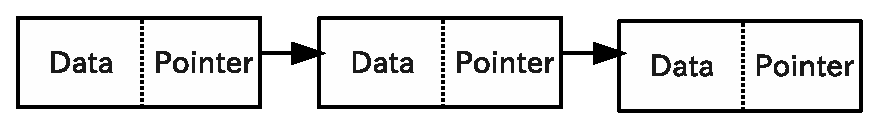
\includegraphics[width=0.75\linewidth,keepaspectratio]{fig13_1.eps}
\caption{片方向リスト}\label{Singly}
\end{figure}

自己参照構造体を複数個用意した後、先頭となるものをひとつ定める。そして、順序付けをポインタを用いて行う。最後の要素のポインタをNULLポインタか先頭要素にしておけば、ターミネータとなる。なお、最後の要素のポインタをNULLにしたものは\textbf{線形リスト}\index{せんけいりすと@線形リスト}(liniarly-linked list)と、先頭要素へのポインタにしたものは\textbf{循環リスト}\index{じゅんかんりすと@循環リスト}(circularly-linked list)と呼ばれている。

\minisec{リストの特徴}
リストに要素を挿入したり、リストから要素を削除するときには、ポインタ部を書き換えることで実現できる。そのため、配列のように多数の要素の書き換えを行う必要がない。これはリストの利点の一つである。

その一方で、メモリ上に連続に配置されているわけではなく、要素番号を用いたアクセスなどができない(ある要素を見つけるために先頭からたどっていく必要がある)ため、配列に比べてアクセスにかかる時間が長くなる。

以上のことからわかるとおり、リストは配列に対し、要素の増減に強く、アクセスに弱いという事になる。そのため、よく増減するようなデータを扱う際などに使うと良い。また、リストはこの後に学ぶグラフのうち、単連結有向グラフの一種でもあるため、グラフの基礎としても使うことができるだろう。
  
\subsection{双方向リスト}
先に学んだ片方向リストでは、次の要素を参照するのは容易であるが、1つ前の要素を参照するのは大変である。そこで、参照のためのポインタを2つに増やし、「次の要素を指すポインタ」と「前の要素を指すポインタ」を準備してやれば、前の要素を参照するのが簡単になるだろう。このように、次の要素と前の要素の両方の参照を持つリストを\textbf{双方向リスト}\index{そうほうこうりすと@双方向リスト}(doubly-linked list)と呼ぶ。図\ref{Doubly}に双方向リストのイメージを示す。
\begin{figure}[htb]
\centering
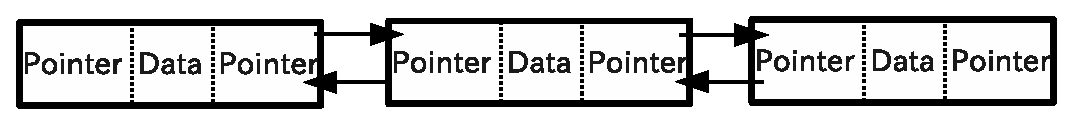
\includegraphics[width=0.95\linewidth,keepaspectratio]{fig13_2.eps}
\caption{双方向リスト}\label{Doubly}
\end{figure}

双方向リストは片方向リストに比べて要素間の行き来が簡単であり、挿入/削除などの容易さもほとんど変わりない。そのため、リストを使う必要性が出てきた場合には双方向リストを使うほうが楽な場合が多いだろう。

\subsection{ループのチェック}
リストにおいて要素間にループがあるかどうかを調べる必要が出てきた時、どのように行えばよいだろうか。片方向リストを例に考えてみよう。
\\ \\ 
一つには、通った要素のログをとっておき、それを参照するという方法がある。だが、これは随分余分にメモリ領域を食ってしまう。あるいは、通った要素に対して、「通ったかどうかのフラグ」をつけ、それが既にオンになっているかどうかをチェックする、という方法もあろう。しかし、これだと、循環のチェック後にフラグをリセットするなどの手間がかかるし、何よりリストに用いた構造体を変更しなければならない(あるいは、リストに用いた構造体をネストとして持つ構造体を作らなければならない)。これらの煩わしい手段を何とかして回避できないものか。

よく知られている方法として、2つのポインタを使う方法がある。リストに用いられている構造体を指すポインタを用意し、共に最初は先頭要素を指しておくものとする。それから、片方のポインタは1つずつ、他方のポインタは2つずつ要素をすすめていく。すると、適切に作られた線形リストならば後者のポインタが先にNULLポインタになるはずである。これがNULLポインタにならず、途中で2つのポインタが出会ってしまう(同じ値を持つ)ようであれば、リストのループが検出されたことになる。この方法は循環リストに使えないように思えるが、循環リストであれば2つのポインタが再び出会う時は先頭要素であるはずである。そのため、この方法を用いればリストが適切に構築されているかどうか、簡単にチェックすることができるのである。

\section{木(Tree)構造}
\textbf{木}\index{き@木}(tree)構造は、「前(親)の要素をひとつだけ持ち、次(子)の要素を複数持つことができる構造」である。各要素のことを\textbf{ノード}\index{のーど@ノード}(node)と呼ぶ。例えば、会社の部署やファイル・ディレクトリの構造などが木構造である。但し、1つの木構造には唯一の「親ノードを持たないノード」が存在し、これを\textbf{根}\index{ね@根}(root)と呼ぶ。逆に、子を持たないノードは\textbf{葉}\index{は@葉}(leaf)と呼ばれる。また、親ノードと子ノードを結ぶ線を\textbf{枝}\index{えだ@枝}(branch)と呼ぶ。図\ref{tree}に木の例を示す。

\begin{figure}[htb]
\centering
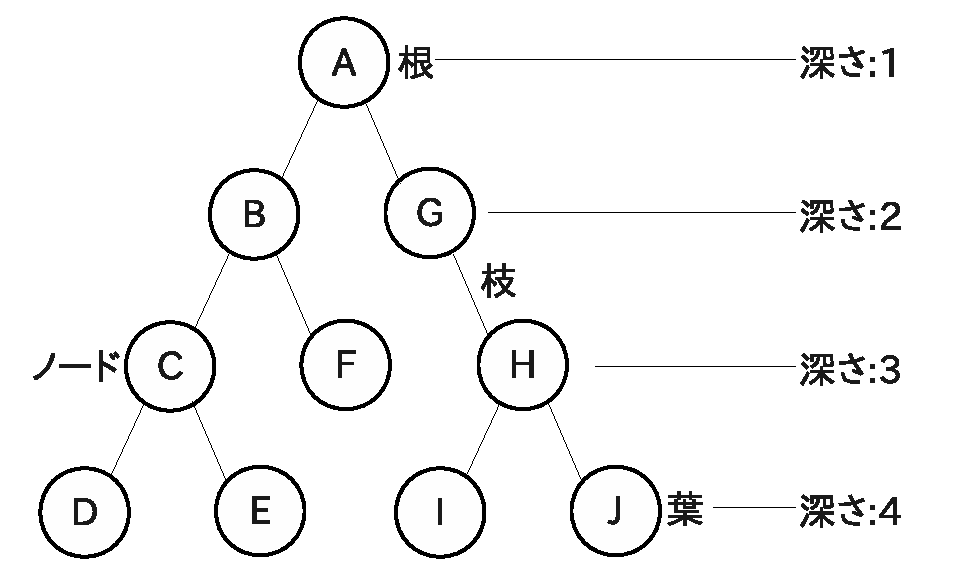
\includegraphics[width=0.8\linewidth,keepaspectratio]{fig13_3.eps}
\caption{木(二分木)の例}\label{tree}
\end{figure}

図\ref{tree}において、「深さ」と記したのは、根を1としてそこから何本の枝でいけるかを足したものであり、そのノードがどの階層に属するかを示している。また、この図を見るとわかるとおり、木はその一部分を取り出しても(例えば、ノードB及びそれ以下に属するノードのみを取り出しても)木構造になっていることがわかる。この、部分を取り出した木のことを\textbf{部分木}\index{ぶぶんぎ@部分木}と呼ぶ。木は、このような再帰的性質故、再帰処理と相性が良い。また、木構造を扱う場合、便宜上左側を先に、右側を後にして説明や実装を行う場合が多く、ここでもこの流儀に乗っ取る。

ここでは、まず木構造の基本となる実装を述べた後、その操作について説明し、そこから派生される幾つかの(基本的な)木構造について触れることとする\footnote{木構造には、ここで紹介する木構造以外にも、BIT(Binary Indexed Tree)・赤黒木・フィボナッチヒープ・セグメント木・スターンブロコット木・スプレー木・B+木等、挙げていくと枚挙に暇がないほどの種類がある。}。

\subsection{二分木}
木の構造の基本を学ぶのに、1つの要素の持つ子要素が最大2個までである\textbf{二分木}\index{にぶんぎ@二分木}(binary tree)を扱う。図\ref{tree}の木も二分木である。要素間の兄弟関係などを利用すれば(深さなどは変わるものの)任意の木を二分木に変換できることが知られているため、二分木について学ぶことは大きな意味を持つ。

二分木のうち、各ノードの子ノードがちょうど2個(葉は0個)であるようなものを\textbf{全二分木}\index{ぜんにぶんぎ@全二分木}(full binary tree)と、更に全ての葉が同じ階層にある全二分木を\textbf{完全二分木}\index{かんぜんにぶんぎ@完全二分木}(complete binary tree)と呼ぶ。図\ref{tree}の木は全二分木ではない(例えばノードGの子は1つである)が、ノードB以下の部分木は全二分木である。
\\ \\ 
二分木は、片方向リストと似たような形で、データ部に子ノードへのポインタ2つを加え
\begin{code}
struct tree_node{
     :
  struct tree_node *left;
  struct tree_node *right;
};
\end{code}
のような構造体を用意すれば実装できる\footnote{この構造体と同様の形式の構造体を双方向リストの実装の際にも用いた。だが、表しているものは全く違う。このように、データ構造とはあくまでもデータの整理の方法であるので、同じ型のものを用いても様々な実装を行うことができる。また、配列を用意し、その番号をポインタ代わりに使うなど、様々な実装を考えることもできるだろう。}。もしも親ノードへの参照が必要な場合は、双方向リストと同様、親ノードへのポインタを追加しても良い。

\subsection{木の探索}
木の全てのノードを調べたい場合がしばしば存在する(\textbf{走査}\index{そうさ@走査}(traversal))。このとき、もれなく重複なく調べる方法として、深さ優先探索と幅優先探索が知られている。
\minisec{深さ優先探索(DFS)}
\textbf{深さ優先探索}\index{ふかさゆうせんたんさく@深さ優先探索}(Depth first search,\textbf{DFS}\index{DFS|see{深さ優先探索}})は、根からスタートし、葉に行き着くまで順に枝を辿り、そこまで行き着いたら戻って別の葉を探索し…という方法である。図\ref{tree}において深さ優先探索をした場合、その経路はアルファベット順になる(左側優先の場合)。

DFSは、「左側の部分木を見る」「右側の部分木を見る」「根を見る」の3つを再帰的に行うことで実装可能である。この時、部分木を見るより前に根を見るDFSを\textbf{行きがけ順}\index{いきがけじゅん@行きがけ順}(preorder traversal)と呼ぶ。その他の順番に対しても名前がついており、左側を見た後右側を見る前に根を見るものを\textbf{通りがけ順}\index{とおりがけじゅん@通りがけ順}(inorder traversal)と、左右を見た後に根を見るものを\textbf{帰りがけ順}\index{かえりがけじゅん@帰りがけ順}(postorder traversal)と呼ぶ。

\minisec{幅優先探索(BFS)}
DFSが左右の木をある種非対称に見ていったのに対し、\textbf{幅優先探索}\index{はばゆうせんたんさく@幅優先探索}(Breadth first search , \textbf{BFS}\index{BFS|see{幅優先探索}})は対称的に見ていく方法である。BFSではキューなどを用いて、同じ階層にあるノードを見ていく。図\ref{tree}の場合、A,B,G,C,F,H,D,E,I,Jのように見ていくことになる。

キューを用いるとはどういうことか、図\ref{tree}を例にもう少し説明を加えておこう。まず根であるAを見る。そしてこの時、「探索すべきもの」として、二つの子ノードB,Gをキューに入れる。次いで、キューの先頭にあるBの要素を見る。そして、やはり同様に、子ノードC,Fをキューに入れる。次にGを見て…と同様のものを繰り返せば良い。
\\ \\ 
以上に説明した探索方法は、後で説明するグラフにも利用されるので、以下にまとめておこう。
\begin{itembox}[l]{DFSとBFS}
\begin{description}
\item[DFS] 根から始まり、そこから行くことができるノードが存在する限り経路をたどる。行くことができなくなったら戻って、戻ってきたノードの別の分岐をたどっていく。一般に再帰を用いて実装される。
\item[BFS] 根から始まり、そこから直接行くことができるノードをキューに入れる。そして、キューの先頭ノードに対し、同様にして、直接いけるノードをキューに入れる。これを繰り返して探索を行う。
\end{description}
\end{itembox}

\subsection{二分ヒープ}
二分木に対して、次の二つの制約を課したものを\textbf{二分ヒープ}\index{にぶんひーぷ@二分ヒープ}(binary heap)あるいは、単にヒープと呼ぶ\footnote{一般の木に対して同様の制約を課したものも\textbf{ヒープ}\index{ひーぷ@ヒープ}(heap)と呼ばれる。}。
\begin{itembox}[l]{(二分)ヒープの制約}
\begin{itemize}
\item 親ノードはそのいずれの子ノードに対しても、一定の大小関係(等号含む)を持つ。すなわち、「親ノード$\ge$子ノード」か「親ノード$\le$子ノード」のいずれか一方が、全ての親子関係について成立する\footnote{もちろん、木の各要素は数値とは限らないので、大小関係はデータに応じてプログラマが定めなければならない。これは後に扱うソートでも同じ事である}。(\textbf{heap property})
\item 構築された木は完全二分木か、最下階層の一段を完全二分木に加えた形になる。この時、最下階層は左側から埋まる。(\textbf{shape property})
\end{itemize}
\end{itembox}

図\ref{heap}にヒープの例を示す。ここでは、大小関係として、アルファベット順に先にあるものを小さいとした。
\begin{figure}[htb]
\centering
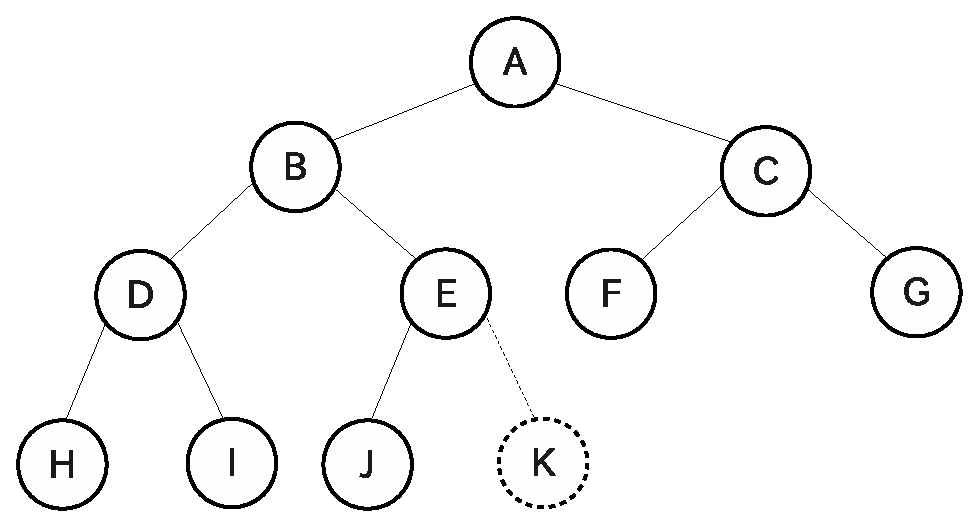
\includegraphics[width=0.8\linewidth,keepaspectratio]{fig13_4.eps}
\caption{ヒープの例(大小関係:アルファベット順に先に来るものが小さい)}\label{heap}
\end{figure}

なお、ヒープは親と子の大小関係については制約を設けているが、子同士の関係には言及していない点に注意しよう。すなわち、左側の子と右側の子の大小関係はどうでもいいのである。これは、二分ヒープに限らず、一般のヒープに言えることである。
\\ \\ 
図\ref{heap}のヒープは、確かに二つの制約を満たしている(そして同時に、偶然にも、左側の子ノードは右側の子ノードよりも小さい)。この関係性により、ヒープはソートや最小値/最大値を求める際によく用いられる。以下、この構築方法について記す。

\minisec{上方移動によるヒープへの要素挿入}
ヒープに新たな要素を加えることを考えよう。この時、図\ref{heap}のノードKのように、今埋まっていない階層の一番左側に新たなノードを追加する。これにより、shape propertyが保たれる。だが、単純に追加しただけではheap propertyが保たれない。

そこで、親ノードと比較し、順序が正しくない場合に親ノードと交換を行う\textbf{上方移動}\index{じょうほういどう@上方移動}(shift up)を行う。もしも、親ノードとの交換が起きた場合、再帰的にこれを実行し、交換が起きなくなるまで交換を繰り返す。これにより、追加ノードはヒープの適切な位置に挿入される。
\\ \\ 
何もない状態から、逐次上方移動によって要素を追加/挿入していけば、ヒープを構築することができる。

\minisec{下方移動によるヒープへの変換}
先程、最初のノードから順に上方移動で順次要素を追加していけばヒープを構築することができると記した。だが、これでは追加の度に再帰を行わなければならず、煩わしい。そこで\textbf{下方移動}\index{かほういどう@下方移動}(shift down)という操作を行い、全データの割り当てられた二分木をヒープへ変換する方法が知られている。
\begin{itembox}[l]{下方移動によるヒープへの変換}
前提として、全データをshape propertyを満たすように二分木に割り当てておく。
\begin{enumerate}
\item ヒープを後方(階層が深い側、同階層では右側)から順に見ていき「葉でないノード」を見つける。このノードを以下親ノードとする。
\item 見つかったノードに対し、子ノードと値を比較し、それらの最小値が親ノードの値となるように(必要に応じて)交換を行う。
\item 再び、最初のステップに戻り、探索を続ける。これを親ノード=根となるまで続ける。
\end{enumerate}
\end{itembox}

ここで紹介した上方移動/下方移動は、各々DFS/BFSと似た様相を呈している。木への操作の基本はDFS/BFSにあるため、再帰やキューといった道具を適切に使えるようにしておくと良い。

\subsection{二分探索木}
ヒープがソートに便利な木であったのに対し、\textbf{二分探索木}\index{にぶんたんさくぎ@二分探索木}(Binary search tree)はその名の通りサーチによく用いられる他、様々に応用がきく構造である。これは、二分木に対し、次の制約を課した木である。
\begin{itembox}[l]{二分探索木の制約}
任意の親ノードに対して
\begin{itemize}
\item その左側の部分木の全要素が、注目している親ノードの値と比べ小さいか等しい。
\item その右側の部分木の全要素が、注目している親ノードの値と比べ大きい。
\end{itemize}
という条件が成立すること。なお、ここでは等しいノードを左側に入れるとしたが、右側に入れても構わない(但し、木全体で左側に入れるか右側に入れるか統一されていなければならない)。
\end{itembox}

上記の制約のため、所定の値を検索する際に素早く検索できるのが二分探索木の特徴である。また、これに対して通りがけ順DFSで値を表示させた場合、昇順ソートされて値が出力される(もちろん、右側を先に持ってくれば降順ソートも可能である)。

\minisec{二分探索木の構築}
二分探索木に要素を追加するにはどうすればよいだろうか。これは、DFS同様に上側から順に見ていけば良い。ここで、注意しなければならないのは、ヒープの追加は下から上に木をたどっていったが、二分探索木では上から下にたどる、という点である。以下、具体的に手順を示そう。
\begin{itembox}[l]{二分探索木への要素の追加}
\begin{enumerate}
\item 最初に根ノードを「現在のノード」として以下の操作を行う。
\item 追加したい値が現在のノードよりも小さいか等しいならば左側へ、大きいならば右側へ進む。
\item 進んだ先にノードが存在しなければそこに追加したい値を新たなノードとして追加して終了する。ノードが存在する場合、そのノードを現在のノードとして、前項に戻る。
\end{enumerate}
\end{itembox}

これにより、最初に適当な根ノードを決め、これに対して順次要素を追加していけば二分探索木が構築できる\footnote{なお、この方法で構築していく時、例えば昇順/降順データが与えられたら、二分探索木は線形リストのような形になってしまう。これを防ぐために用いられるのが赤黒木などの平衡二分探索木である。本書では紙数の都合上扱わないが、興味があれば学んでみて欲しい。}。同様にして、二分探索木を用いてのサーチを行うこともできる。

\minisec{ノードの削除}
ここまではノードの追加/木の構築について話してきたが、必要なくなった要素は木から削除しなければならない。ヒープの場合、削除したい場所に最後のノードを移動し、大小関係について整合性を取れば良い(上方/下方移動)のであるが、二分探索木からの削除は少し面倒である。
\begin{itembox}[l]{二分探索木からのノードの削除}
\begin{enumerate}
\item 最初に根ノードを「現在のノード」として以下の操作を行う。
\item 現在のノードと、削除を行う値を比較する。この時、削除する値が現在のノードと等しければステップ4に進む。等しくない場合、削除する値が現在のノードよりも小さければ左側に、そうでなければ右側に移動し、次項へ進む。
\item 進んだ先のノードを現在のノードとして、前項へ戻る。
\item 現在のノードが子ノードを持たない場合はそのノードを削除して終了する。子ノードを持つ場合、削除した後に次項に進む。
\item 子ノードを1つだけ持つ場合は削除した場所を、子ノードによって置き換えて終了する。2つ持つ場合は削除したノードの右側部分木の最小値のノードで置き換える。この時、置き換え元(最小値)のノードに右側子ノードが存在するならば、右側子ノードを置き換え元ノードに置き換える(以下の関係は保つ)。
\end{enumerate}
\end{itembox}

\section{グラフ}
リンクリストは「前のノードが1つ・次のノードが1つ」というデータ構造であった。木は「前のノードが1つ・次のノードが複数」というデータ構造であった。この自然な拡張として、「前のノードが複数・次のノードが複数」というデータ構造を考えることができる。あるいは、前後の区別をなくし「隣り合ったノードが複数」という事もできる。路線図やロードマップ・地図のようなものがこのようなデータ構造をなしている。前後の区別をするならば、例えばロードマップの場合、一方通行の道路があったらそこには指向性がある。前後の区別をしないものとしては、例えば地図が考えられる。地図を見てみると兵庫県は京都府・大阪府・和歌山県・鳥取県・岡山県・徳島県・香川県と接しているが、これは接していることだけに意味があり、兵庫県から京都府へ方向付けする必要性はない。ここでは、「複数のノードが隣り合っているデータ構造」であるグラフを扱う。

\subsection{グラフの基礎概念}
\textbf{グラフ}\index{ぐらふ@グラフ}(graph)とは、\textbf{ノード}\index{のーど@ノード}(node,路線図でいう所の駅に当たるもの。日本語では\textbf{節点}\index{せつてん@節点|see{ノード}}ないし\textbf{頂点}\index{ちょうてん@頂点|see{ノード}}と呼ぶ。)とそれらをつなぐ\textbf{エッジ}\index{えっじ@エッジ}(edge,日本語では\textbf{辺}\index{へん@辺|see{エッジ}}。路線図でいう所の駅の間の線路に当たるもの。)からなるデータ関係をいう。図\ref{graph}にグラフの例を示す。

\begin{figure}[htb]
\centering
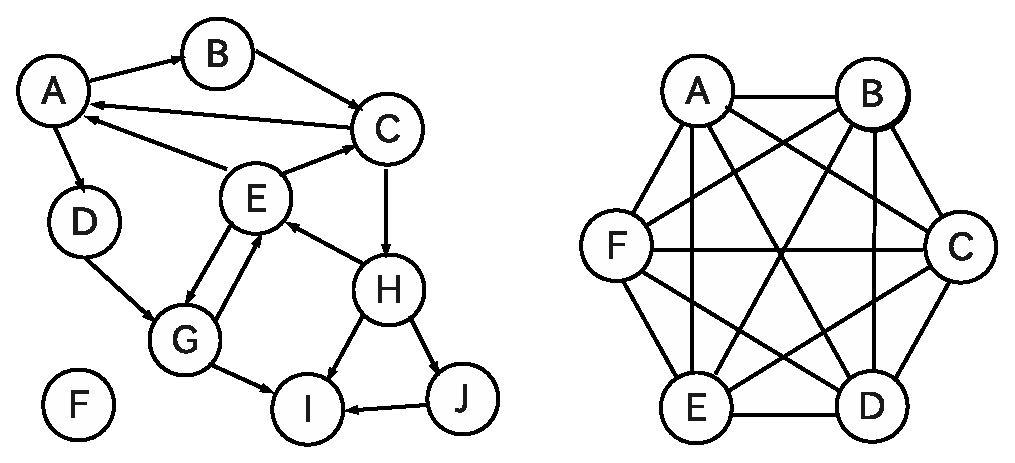
\includegraphics[width=0.9\linewidth,keepaspectratio]{fig13_5.eps}
\caption{グラフの例(左:有向グラフ・右:無向グラフ)}\label{graph}
\end{figure}

図\ref{graph}の左側のように、辺に指向性があるものを\textbf{有向グラフ}\index{ゆうこうぐらふ@有向グラフ}(digraph)と呼ぶ。これに対し、図\ref{graph}の右側のような、辺に指向性がないものは\textbf{無向グラフ}\index{むこうぐらふ@無向グラフ}(undirected graph)と呼ばれる。
\\ \\ 
グラフの各々の辺には方向づけを行うことができるが、それに加え\textbf{重み}\index{おもみ@(辺の)重み}を付けることができる。例えば路線図では、A-B間は3分、A-D間は2分、B-D間は4分などと所要時間を付けることができるが、この所要時間を辺毎にのせていけば、これが辺の重みになる。ここで挙げた路線図の場合は向きに寄って時間が変わったり一方通行だったりすることはないだろうが、ロードマップの場合は混雑の度合いによって所要時間がA→Bは30分、B→Aは25分などのように指向性を持つ場合があり、このような場合には有向グラフを用いることになる。ここでは重みを所要時間とした為、重みは正または0だろうが、実際には負の値を取る重みも存在する\footnote{負の値を取る重みなど、理論はともかく実際には何の役に立つのか?と思うかもしれない。だが、辺の途中でものの授受などがある場合は正負両方が必要だろう。例えば実生活でも、どこかに行く経路をたどる時、途中で銀行のある道でお金をおろすならば、その道ではお金がプラスになる。だが、お金を払わなければいけない道(有料道路など)があればお金はマイナスになるだろう。}。

\minisec{グラフの種類}
グラフには、その特徴に応じて幾つかの種類がある。ここではそれを紹介しておく。
\\ \\ 
無向グラフにおいて、任意の2ノード間に経路が存在するグラフのことを\textbf{連結グラフ}\index{れんけつぐらふ@連結グラフ}(connected graph)と呼ぶ。グラフを扱う場合、連結性を確かめてから使う場合が多い(チェックについては次項に述べる)。また、連結グラフでなくとも、適切な部分グラフに分ければ、連結グラフに分けて扱える。

図\ref{graph}右のように、全てのノードの間にエッジがあるようなグラフを\textbf{完全グラフ}\index{かんぜんぐらふ@完全グラフ}(complete graph)と呼ぶ。自己ループや多重辺(ある2ノード間に複数の同方向エッジが存在するもの)を含まない\textbf{単純グラフ}\index{たんじゅんぐらふ@単純グラフ}(simple graph)を扱うアルゴリズムを考える時、完全グラフはエッジの数が最大化されたグラフとして扱えるため、「エッジの多い場合の極端な例」としてしばしば用いられる。ノード数$V$の完全グラフに対して、そのエッジ数$E$は
\begin{equation}
E=\frac{V(V-1)}{2}
\end{equation}
により計算することができる。
\\ \\ 
また、閉路(ループ)を持たないグラフにも特別な名前が付いている。閉路を持たない連結グラフは、書いてみればわかるが、前述の木である。木をグラフとしてみた時、完全グラフとは逆にエッジ数が一番少ないため、「エッジの少ない場合の極端な例」として使うことができる。ノード数$V$の木に対してそのエッジ数$E$は
\begin{equation}
E=V-1
\end{equation}
である。

一方、閉路を持たない非連結グラフは、木が多く集まった形をなすことから\textbf{森}\index{もり@森}(forest)と呼ぶ。
\\ \\ 
以下では、無向単純グラフを基本に説明を行うこととし、単に「グラフ」と書いた場合は無向単純グラフを指すこととする。有向グラフの場合にも多少工夫することで同様のアルゴリズムを適用できる場合が多い。

\subsection{グラフの実装と連結性チェック}
ここでは、グラフを実装し、その連結性をチェックすることについて説明する。これは、グラフに関する諸問題の基礎となる部分である。
\minisec{隣接行列/接続行列による表現}
グラフを実装する場合、リストや木で用いたような構造体表現も可能であるが、重みやノード毎に個数が違う等の面倒な部分もある(有向グラフの場合は指向性の表現も面倒)。エッジ数が少ない場合は構造体表現も楽であるが、増えてきた場合(特に完全グラフの場合)は構造体表現は面倒である。そこで、グラフのノードを配列を用いて用意しておき、エッジに対し\textbf{隣接行列}\index{りんせつぎょうれつ@隣接行列}(Adjacency matrix)と呼ばれる行列を用いることが多い。

隣接行列は二次元配列を用いて実装される。隣接行列の\verb|[i][j]|成分をノード\verb|i|からノード\verb|j|への辺の重みとする。辺が存在しない場合は、それを表す値を代入しておく。重みがないグラフについては、1/0を辺の有無に対応させて用いる場合が多い。
\\ \\ 
また、別の実装として、ある点からある辺が出ているかどうかについて\textbf{接続行列}\index{せつぞくぎょうれつ@接続行列}(incidence matrix)を用いることもある。これは\verb|[i][j]|成分をノード\verb|i|からエッジ\verb|j|が出ているかどうかに対応させた行列である。単純グラフを扱う場合、この行列では1列にちょうど2個の1(ノードからエッジが出ている値)が見つかるはずである。

\minisec{グラフの連結性チェック}
グラフが連結であるかどうかは、アルゴリズムが適用できるかどうかを始めとして、様々な場面で重要である。ここではグラフの連結性を調べる方法について述べる。

グラフが連結であるということは、先に述べたとおり「任意の2ノード間に経路が存在する」ということである。ここで、無向グラフにおいてはある1ノードから全てのノードに到達可能である場合、他のノードからも全てのノードに到達可能であるという点に着目する。すると、ある1点から全ての点にエッジをたどって到達可能であるかどうかを調べれば良い、という結論に至る。
\\ \\ 
では、到達可能かどうかはどのように判定すればよいか。これは、実際にある1ノードから「もれなく・重複なく」たどってみれば良い。DFSないしBFSの出番である。各ノードが到達可能かどうかを表す一連のフラグ配列を用意し、これに可能であるかどうかを調べていけば良いのである。DFSを再帰処理で組むのは変わらないが、BFSの場合、キューを用いずとも、フラグ配列を順に見て行って、まだ見ていないノードを見れば良い。

同様に、連結性のチェックに限らず、グラフを探索する場合にはDFSかBFSのいずれかを用いるのが基本となる。
\\ \\ 
この後に話す最短路問題・閉路問題では連結グラフを前提とし、特段の記述がない場合非連結グラフは扱わない。

\subsection{最短路問題}
\textbf{最短路問題}\index{さいたんろもんだい@最短路問題}(Shortest path problem)とは、重み付きグラフにおいて、あるノードから別ノードへの道のうち重みを最小化するものを求める問題である。この内、ある2点間の最短路を求める問題は\textbf{2頂点対最短路問題}\index{にちょうてんついさいたんろもんだい@2頂点対最短路問題}と、単一の始点から全ての点への最短路を求める問題は\textbf{単一始点最短路問題}\index{たんいつしてんさいたんろもんだい@単一始点最短路問題}と、全ての点対について最短路を求める問題を\textbf{全点対最短路問題}\index{ぜんてんついさいたんろもんだい@全点対最短路問題}と呼ぶ。ここでは、図\ref{shortest}のグラフを例に、単一始点最短路問題と全点対最短路問題のアルゴリズムを紹介する\footnote{2頂点対最短路問題については、単一始点最短路問題のアルゴリズムを用いて求めれば良い}。

\begin{figure}[htb]
\centering
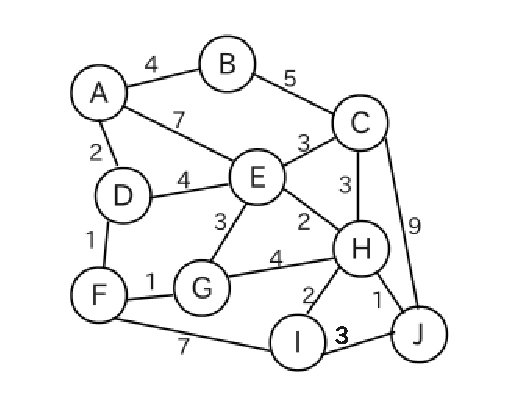
\includegraphics[width=0.5\linewidth,keepaspectratio]{fig13_6.eps}
\caption{重み付き無向グラフ}\label{shortest}
\end{figure}

なお、以下では最短路のコストを求めているが、最短路そのものを求める(経路復元)場合も同様のアルゴリズムで直前の頂点を記憶しておけば良い。もちろん、コストを求めてからBFS/DFSなどをしても求められる。

\minisec{Bellman-Ford法}
図\ref{shortest}の始点Aからの単一始点最短路問題を考えよう。ノード$i,j$を結ぶエッジの重みを$C_{i,j}$で表し\footnote{無向グラフの場合、$C_{i,j}=C_{j,i}$であるが、有向グラフでは区別する。また、ノード$i,j$間にエッジが存在しない場合、$C_{i,j}$は充分大きな値とする(実装では大きな値だが、理論上は$C_{i,j}=\infty$としても良い)。}、Aからノード$k$への最短距離(最小重み)を$D_k$として、次のような等式が成立する。
\begin{equation}
D_i=\min_j\left(D_j+C_{i,j}\right) \label{bellman}
\end{equation}

木の場合、式(\ref{bellman})を初期条件$D_A=0$の下で順次計算していけば全ての点への最短路が求められる。しかし、グラフに閉路が含まれる場合などは「順次」の順序を決めることができない。そこで、$D_A=0,D_{i(\neq A)}=\infty$として、式(\ref{bellman})を適用し、値を更新していく。この手法を\textbf{Bellman-Ford法}\index{Bellman-Fordほう@Bellman-Ford法}と呼ぶ。手順をまとめると次のようになる。
\begin{itembox}[l]{Bellman-Fordのアルゴリズム}
\begin{enumerate}
\item 初期化:スタートノードの値(最小コスト候補)を0、他のノードの値を$\infty$(充分大きな値)に設定する。
\item 各エッジに対して式(\ref{bellman})を適用して、その隣点からの最短距離更新がないかをチェックし、現在の「仮の最短距離」よりも小さければ更新する。
\item 前ステップを、更新がなくなるまで繰り返す。この反復は高々頂点数-1回で終わる。
\end{enumerate}
\end{itembox}

ノード数$V$、エッジ数$E$のグラフに対して、この時間計算量は$O(VE)$である。なお、時間計算量については次講か姉妹書の実習編を参照されたい。
\\ \\ 
負の重みを持つエッジ(有向グラフの場合は負の閉路)が存在した場合、最短経路は存在しない(その閉路を繰り返し通ることで無限に小さくできるため)。しかし、このケースでは、Bellman-Ford法が頂点数-1回の反復で終了しないため、それにより負閉路を検出することが可能である。これは、次に述べるDijkstra法にはない利点である。

\minisec{Dijkstra法}
Bellman-Ford法では、一度エッジを計算しても、その点への最短距離が定まるかどうかはわからなかった。そのため、更新を何度も繰り返した。だが、図\ref{shortest}のノードDへの最短路は、ノードAから出るエッジの重みなどを考慮すれば、$D_D=2$であると直ちにわかる。同様の論法で、$D_F=3,D_B=4,D_G=4$と、順次最短路を確定させていくことができる。そして、確定したノードへのエッジについては、もうこれ以上考慮に入れる必要はなくなる。これにより、Bellman-Ford法から無駄を省いた方法が次の\textbf{Dijkstra法}\index{Dijkstraほう@Dijkstra法}\footnote{このDijkstra(ダイクストラ)は構造化プログラミングの提唱者として知られているエドガー・ダイクストラその人である。}である。
\begin{itembox}[l]{Dijkstraのアルゴリズム}
\begin{enumerate}
\item 初期化:スタートノードの値を0、他のノードの値を未定義(または$\infty$)に設定する。
\item 確定ノードをピックアップできなくなるまで(=変化がなくなるまで)次の3,4のループを繰り返す。但し、最初の確定ノードはスタートノードとする。
\item 確定ノードから伸びているエッジをそれぞれチェックし、式(\ref{bellman})により現在の最小コストを計算し、そのノードの現在値よりも小さければ更新する。
\item まだ確定されていないノードのうち、最小の値を持つノードを見つけ、確定ノードとする(確定フラグを立てる)。
\end{enumerate}
\end{itembox}

Dijkstra法を図\ref{shortest}に適用した場合、確定ノードはA,D,F,(B,G),E,H,(C,J),Iの順に定まる。但し、括弧でくくったノードの順番は入れ替わることがある。
\\ \\ 
Dijkstra法は「現在の最小値はこれ以上更新されない」という考えに従うため、更新が起こりうる負のエッジを持つグラフ(有向・無向を問わない)については適用できない。また、ノード数$V$、エッジ数$E$のグラフに対して、Dijkstra法により最短路を求めるための時間計算量は$O(V^2)$である。ただし、これは確定ノードを決定する際に、ループを回して全てのノードをチェックするからであり、ここをヒープ(またはプライオリティーキュー)を用いて管理するとより速くなる。以下、これについて述べる。
\\ \\ 
スタートノードを根としたヒープを考えよう。ここでは簡単のため、図\ref{heap}の各ノードの文字と、図\ref{shortest}の各ノードの文字が対応していることにし、ヒープの各ノードには$D_i$の値を割り当てておくことにする。

ノードAに隣接しているノードを考えれば、$D_D,D_B,D_E$の更新が起こる。この更新を行った後、ヒープのノードAを削除する(削除方法は既に述べた)。そして根ノードとなったノードを確定ノードとし、同様の処理を施していけば良い。まとめると、次のようになる。
\begin{itembox}[l]{Dijkstraのアルゴリズム(ヒープ利用)}
\begin{enumerate}
\item 初期化:スタートノードの値を0、他のノードの値を未定義(または$\infty$)に設定する。
\item ヒープ初期化:最短距離の値についてのヒープを構築する。この際、ヒープのデータは、元のグラフのどのノードに対応しているかという事と、最短距離の値である。
\item ヒープのノードが尽きる(または1つになる)まで、次の4〜6の操作を繰り返す。
\item ヒープの根ノードに対応するグラフのノードを確定ノードとする。
\item 確定ノードから伸びているエッジをそれぞれチェックし、式(\ref{bellman})により現在の最小コストを計算し、そのノードの現在値よりも小さければ更新する。
\item ヒープから根ノードを削除し、更新した値を用いてヒープを再構築する。
\end{enumerate}
\end{itembox}

この方法を用いると確定ノードを速く決められる事になるため、時間計算量が$O(E\log V)$となる。これは、Bellman-Ford法に比べて速い方法である。そのため、最短路を定めることが可能な無向グラフや、負エッジを有しない有向グラフについてはDijkstra法が用いられることが多い。
\\ \\ 
なお、全てのエッジのコストが等しい場合には、単にBFSを用いてエッジ数を記録していったほうが簡単に経路を求められる。

\minisec{Warshall-Floyd法}
全点対最短路問題を解く場合には、各ノードに対する単一始点最短路問題をBellman-Ford法やDijkstra法により解いてもよいが、一般化した\textbf{Warshall-Floyd法}\index{Warshall-Floydほう@Warshall-Floyd法}を用いることが多い。この方法は、先の2つのアルゴリズムと違った漸化式を用いる(漸化式を作って計算する、\textbf{動的計画法}\index{どうてきけいかくほう@動的計画法}(Dynamic Programming,\textbf{DP}\index{DP|see{動的計画法}})の一種である)。

頂点に0-indexedにより番号をつける。第$k$番までの頂点及びノード$i,j$そのものを用いて構築可能な、ノード$i,j$間の最短経路を$D_{i,j,k}$と表すと、次の関係式が成立する。
\begin{equation}
D_{i,j,k+1}=\min(D_{i,j,k},D_{i,k+1,k}+D_{k+1,j,k}) \label{warshall}
\end{equation}
従って、この漸化式に対し、適切な初期値を定めて計算を実行すれば良い。初期値は
\begin{equation}
D_{i,j,0}=\min(C_{i,j},C_{i,0}+C_{0,j})
\end{equation}
とすれば良い(但し、$C_{i,j}$はノード$i,j$を結ぶエッジの重みで、存在しなければ$\infty$)。これをコードにまとめると次のようになる。なお、実際の実装の際には、$D_{i,j,k}$のうち、$k$を落としてしまって良い。
\begin{itembox}[l]{Warshall-Floydのアルゴリズムの実装}
\verb|i,j,k|はint型とし、式(\ref{warshall})に示したのと同じ意味を持つものとする。\verb|V|はグラフの頂点数で、\verb|D[i][j]|は$D_{i,j,k}$を表すものとする。また、\verb|C[i][j]|は隣接行列である。
\begin{lstlisting}[caption=Warshall-Floydのアルゴリズム,label=program13_3]
#define MIN(x,y) (((x)<(y))?(x):(y))

// initializing
  for(i=0;i<V;i++) for(j=0;j<V;j++) D[i][j]=MIN(C[i][j],C[i][0]+C[0][j]);
 
//calculation 
  for(k=1;k<V;k++) for(i=0;i<V;i++) for(j=0;j<V;j++)
                                        D[i][j]=MIN(D[i][j],D[i][k]+D[k][j]);
\end{lstlisting}
ここに示したコード断片により、\verb|D[i][j]|にノード$i,j$間の最短距離が入る。
\end{itembox}

ノード数$V$,エッジ数$E$のグラフに対して、Warshall-Floyd法は$O(V^3)$で動作する。Bellman-Ford法を全ノードに用いた場合$O(V^2E)$、Dijkstra法の場合$O(VE\log V)$であることを考えると、とりわけ、エッジ数が多いグラフに対して速いことがわかる。また、比較的実装が簡単なのも利点である。
\\ \\ 
さらに、Warshall-Floyd法は、負エッジを持つ有向グラフにも適用できる他、負閉路(無向グラフの場合負エッジ)の検出も可能である(\verb|D[i][i]|が負になる)。

\subsection{閉路問題}
グラフ理論の古典的な問題として閉路問題を紹介する。
\minisec{頂点の次数}
閉路問題の前に、ノードの\textbf{次数}\index{じすう@(ノードの)次数}という概念を導入する。各ノードに対し、それに接続しているエッジの数を次数と呼んでいる。有向グラフの場合、ノードに入ってくる辺の数を\textbf{入次数}\index{いりじすう@入次数}と、ノードから出ていく辺の数を\textbf{出次数}\index{しゅつじすう@出次数}と呼ぶ。

\minisec{オイラー閉路問題と一筆書き}
閉路問題は大きくわけて2つにわけられる。まず、全ての辺を1度ずつ通るような閉路である\textbf{オイラー閉路}\index{おいらーへいろ@オイラー閉路}(Eulerian cycle)について説明する。

与えられたグラフがオイラー閉路であるかどうか(このようなグラフを\textbf{オイラーグラフ}\index{おいらーぐらふ@オイラーグラフ}(Eulerian graph)と呼ぶ)は、次の定理により判定することができる。
\begin{itembox}[l]{オイラーグラフ}
与えられたグラフがオイラーグラフであることは、全ノードの次数が偶数であることと同値である。
\end{itembox}
\\ \\ 
オイラー閉路問題を言い換えると、スタート地点とゴール地点が同じ一筆書きでそのグラフを書くことができるかどうか\footnote{この問題の最も古典的な例として\textbf{ケーニヒスベルグの橋}が知られている。}の判定である。一方、現在よく考えられる一筆書きには、例えば数字の9のように、最初の点と最後の点が等しくないような場合もある。このような「一筆書き問題」の判定も考えてみよう。

一般に、一筆書き可能なグラフのことを\textbf{オイラー路}\index{おいらーろ@オイラー路}(Eulerian path)と呼ぶ。オイラー閉路は当然オイラー路でもある。オイラー路でありオイラー閉路でないようなグラフ(\textbf{準オイラーグラフ}\index{じゅんおいらーぐらふ@準オイラーグラフ}(semi-Eulerian graph))は、次のように判定できる。
\begin{itembox}[l]{準オイラーグラフ}
与えられたグラフが準オイラーグラフであることは、全ノードのうちに次数が奇数であるものがちょうど2つ存在する事と同値である。
\end{itembox}

以上から、一筆書き可能かどうかは、グラフにおいて全ノードのうち、次数が奇数であるものが存在しないか2つ存在するかによって判定可能である。なお、オイラーグラフの始点(=終点)はどこでもよいが、準オイラーグラフの始点と終点は、次数が奇数である2つのノードである。

\minisec{ハミルトン閉路問題と巡回セールスマン問題}
オイラー閉路が全辺を通る問題だったのに対し、\textbf{ハミルトン閉路}\index{はみるとんへいろ@ハミルトン閉路}(Hamiltonian cycle)は全ての頂点を1度ずつ通るような閉路の事を言う。閉路でないが全ての頂点を1度ずつ通るような路を\textbf{ハミルトン路}\index{はみるとんろ@ハミルトン路}(Hamiltonian path)と呼ぶのは、オイラー路と同様である。

与えられたグラフが、ハミルトン閉路を\underline{含む}場合、そのグラフを\textbf{ハミルトングラフ}\index{はみるとんぐらふ@ハミルトングラフ}(Hamiltonian graph)と、ハミルトン路を含むがハミルトン閉路を含まないグラフを\textbf{準ハミルトングラフ}\index{じゅんはみるとんぐらふ@準ハミルトングラフ}(semi-Hamiltonian graph)と呼ぶ。オイラーグラフはグラフそのものであったが、ハミルトングラフは含むかどうかである点に注意されたい。
\\ \\ 
あるグラフがハミルトングラフであるかどうか判定するハミルトン閉路問題を効率よく解くアルゴリズムはない。ハミルトン路を含むかどうかの判定は、それ以上に難しいとされる。さらに、ハミルトン閉路問題に重みをつけた、「ハミルトン閉路のうち最短路を求めよ」という問題は\textbf{巡回セールスマン問題}(Traveling Salesman Problem,\textbf{TSP})として知られる難問である。ハミルトン閉路問題はClass-NP(後述)に属するが、ハミルトン路問題や巡回セールスマン問題はClass-NPにすら属さない(丸つけすら難しい)可能性のある問題であり、オイラー閉路同様に古典的であるが、難易度は雲泥の差である。
\\ \\ 
ここまで、グラフについて古典的な問題を扱ったが、グラフの問題には、彩色問題・マッチング・フロー問題・最小全域木など、まだまだ多くの問題が存在する。詳しくはグラフ理論の専門書\footnote{例えば、「シリーズ 情報科学の数学 グラフ理論」(恵羅,土屋 1997 産業図書)などがある。}を参照されたい。

\newpage
\begin{shadebox}
\section*{本講の要点}
本講では、データを適切に整理して扱うために、基本的なデータ構造を学んだ。
\subsection*{基本的なデータ構造}
\begin{itemize}
\item スタックはLIFO、キューはLILOのデータ構造である。
\end{itemize}

\subsection*{リンクリスト}
\begin{itemize}
\item リンクリストは、ポインタを用いてデータの順序関係を示し、データの挿入や削除を容易にしたものである。
\item リンクリストの各要素は最大1つまでの前要素/次要素を持つ。
\item リンクリストを実装する場合には自己参照構造体を用いる。
\item リンクリストに循環が存在するかどうかは、2つのポインタを「おいかけっこ」させることにより判定できる。
\end{itemize}

\subsection*{木}
\begin{itemize}
\item 木構造は前要素を1つ以下、次要素を複数持つデータ構造である。
\item 任意の木は、前要素1つ以下、次要素2つ以下の二分木に変換できる。
\item 木の探索(走査)方法はDFSとBFSが知られている。
\item ノード間あるいは木全体に制約をかけることで、ヒープや二分探索木といった様々な木を実装できる。
\end{itemize}

\subsection*{グラフ}
\begin{itemize}
\item グラフは前要素・次要素ともに複数持つデータ構造である。前後の区別をなくしたものもある。
\item グラフが連結しているかどうかは様々な問題の基礎になる。連結の判定はBFSやDFSによる。
\item 重み付きエッジを持つグラフに対し、そのノード間の最小重みを求める問題を最短路問題と呼んでいる。最短路問題にはBellman-Ford法・Dijkstra法・Warshall-Floyd法などの方法が知られている。
\item 閉路問題は大きくオイラー閉路とハミルトン閉路に分かれる。前者は次数を数えることで判定可能であるが、後者は簡単には解けない。
\end{itemize}

\end{shadebox}


\chapter{ソートとサーチ}
ソートは、ある程度慣れたプログラマであれば常識として知っておいても良いアルゴリズムで、活用される場面も少なくない。また、アルゴリズムの解析においても、典型的かつ動作が見やすくイメージしやすいため、非常によく用いられる例である。本講では様々なソートを知り、アルゴリズムの解析手法についても学ぶと共に、これと関連の深い配列の探索についても学ぶ。ソート、サーチの世界はそれだけで分厚い本が書けるほどに奥深く\footnote{具体的には「The Art of Computer Programming Volume 3」(D.E.Knuth著、有澤 誠他訳、ASCII、2006)。ソート・サーチについてはこの本1冊で万全であると言って過言でない名著。}とても1講で解説しきれるものではないが、ここで素地だけでも学んでおくことが後々役立つと考えている。
\section{ソート総論}
個々のソートを見ていく前に、ソート全体について説明する。
\subsection{ソートとは何か}
\textbf{ソート}\index{そーと@ソート}(Sort)は、日本語では「整列」や「並び替え」と訳され、データをある一定の規則に従って並び替えることを言う。ソートの方法は多数存在し、それぞれに特徴がある。

この章のソートの部分では、代表的なソートのアルゴリズムのみを紹介し、紙数の関係上実装は行わない。そのため、これまでの復習として自力で実装してみていただきたい。なお、特別に断らない限り、ソート対象を要素数$n$のint型配列、ソート規則を昇順(小さい数が前)として説明を行う。
\subsection{ソートの解析〜バブルソートを例に〜}
アルゴリズムの解析について、本書ではここまで全く書いてこなかったので、ここでバブルソートを例に解析法を紹介しておく。なお、演習編では最初にアルゴリズムの解析について掲載したので、合わせて参照されたい。
\\ \\ 
\textbf{バブルソート}\index{ばぶるそーと@バブルソート}(Bubble Sort)は、配列を前から順に見ていって、その大小関係がひっくり返っている場所をスワップすることで整列を行う方法である。例えば[4,1,3,2,3]のバブルソートを考えると、[1,4,3,2,3]$\rightarrow$[1,3,4,2,3]$\rightarrow$[1,3,2,4,3]$\rightarrow$[1,3,2,3,4]$\rightarrow$[1,2,3,3,4]というソート手順になる。小さい要素が泡のように上(前)にやってくることから、この名前がついた。

\minisec{時間計算量と空間計算量}
さて、バブルソートの特徴として、配列を一度スキャンし終えると、最大の要素が配列の末尾に来ることが挙げられる。そのため、今度は配列より1小さい数の比較ですむ。これを繰り返していくと、比較回数は$\frac{n(n+1)}{2}$回であり、交換回数は最大$\frac{n(n+1)}{2}$回であることがわかるだろう。このことから、バブルソートのアルゴリズムの計算回数は、$n$の二次関数に比例して大きくなっていくことがわかる。つまり、バブルソートにかかる時間は、十分$n$が大きい時、「高々」$n^2$に比例する程度である。これを$O(n^2)$のアルゴリズムと記す。
\\ \\ 
ここで用いた$O$による記法を\textbf{ランダウの漸近記法}\index{らんだうのぜんきんきほう@ランダウの漸近記法}(Landau asymptotic notation)とよぶ。なお、ここでは「高々」の評価としたが、同じく$n$が十分大きい時ちょうど$f(n)$に比例するようなら$\Theta\left(f(n)\right)$と、少なくとも$g(n)$に比例するようなら$\Omega\left(g(n)\right)$と記す。以下では原則$O$を用いる。

また、これらの$O,\Theta,\Omega$は何れも使われるメモリの量を記すときにも使える。バブルソートの場合、元の配列以外で余分に使うメモリはせいぜい交換用の変数ぐらいで、$n$によらないので$O(1)$のメモリ量である。
\\ \\ 
ここに述べた、計算回数のオーダーは一般に\textbf{時間計算量}\index{じかんけいさんりょう@時間計算量}(time complexity)と、メモリ量のオーダーは\textbf{空間計算量}\index{くうかんけいさんりょう@空間計算量}(space complexity)と呼ばれている。また、$O(1)$は\textbf{定数オーダー}\index{ていすうおーだー@定数オーダー}と、$O(\ln n)$は\textbf{対数オーダー}\index{たいすうおーだー@対数オーダー}と、$O(n^k)$は\textbf{多項式オーダー}\index{たこうしきおーだー@多項式オーダー}\footnote{ある問題に対し、その解を多項式時間で求められる問題を\textbf{Class-P}\index{Class-P}(P:Polynomial time)の問題と呼ぶ。また、ある問題の解の候補が与えられた時、それが解として正答かどうかを判定するのに多項式時間で判定できるものを\textbf{Class-NP}\index{Class-NP}(NP:Non-deterministic Polynomial time)の問題と呼ぶ。わかりやすく言うと、多項式時間で解ける問題がClass-P、多項式時間で丸付けのできる問題がClass-NPである。アメリカ・クレイ研究所のミレニアム懸賞問題の中には、これにまつわる問題として\textbf{P対NP問題}がある。この問題は、Class-NPに属する問題は必ずClass-Pに属するか?という問題である(逆にClass-Pの問題がClass-NPに属することは直感からも明らかだろう)。興味があれば調べてみて欲しい。}と、$O(e^n)$は\textbf{指数オーダー}\index{しすうおーだー@指数オーダー}と呼ばれる。時間計算量にこれらのオーダーが用いられた場合「○○オーダーの時間」と呼ぶのは煩わしいので「指数時間」などと呼ばれる。

オーダーについて注意しなければならない点として、十分大きい値での比例関係での等号なので定数倍やよりオーダーの小さい項があったとしてもこれらは同じオーダーである、という点が挙げられる。例えば、$O(n^3)$と$O(5n^3)$と$O(3n^3+2n^2+\log n)$は同じオーダーである。
\\ \\ 
ここで紹介した時間計算量や空間計算量は決して理論だけのものではない。実装方法を決める際に、求められている仕ように対して時間計算量/空間計算量を見積もることで、適切な実装を選ぶ一助とすることができる。主要な処理のオーダーを知っておけば、全体の見通しを立てやすい(例えば、strlen関数は、引数の文字列長$l$に対し、各回の呼び出し〜返却まで$O(l)$かかることが知られている)。また、計算回数を大雑把でよいので見積もれば、処理にかかる時間等も把握しやすい\footnote{現在のPCなら、大体1000万回〜1億回の処理で1秒である(1回の処理にかかる時間やPC性能により変動)。もちろん、計算時間を小さい$n$について測定し、そこから大きい$n$についての時間を推定するという手法も有効である。}。

\minisec{ソートの安定性}
バブルソートでは、最初に2つあった3の順序関係が入れ替わっていない。このように、同じ大きさの値が配列にある時、その順序関係が入れ替わらないソートを\textbf{安定なソート}\index{あんていなそーと@安定なソート}(Stable sort)と呼び、逆に入れ替わるソートを\textbf{不安定なソート}\index{ふあんていなそーと@不安定なソート}(Unstable sort)と呼ぶ。単なる値の整列だけならば気にしなくてよいが、構造体や文字列をソートする場合には安定性が問題になってくる場合がある。ソートによっては、不安定であっても比較的簡単に安定に組みなおすことが可能なものもある。

\minisec{バブルソートのまとめ}
以上に説明したバブルソートについてまとめておこう。なお、バブルソートは速度も遅く、これといった優位性も無いので、実装練習以外に使われることは稀である。
\begin{itembox}[l]{バブルソート}
\minisec{手順}
\begin{enumerate}
\item 配列を順にスキャンし、途中、大小関係が逆転している部分があれば、その2要素を交換する。
\item 第$k$回目のスキャンにおいて第$n-k+1$要素までスキャンを終えたら\footnote{効率化を考えて第$n-k+1$要素までとしたが、第$n$要素まで見るとする方が一般的である。もちろん、第$n$要素まで見るほうが遅い。}、1に戻る。但し、ソートが完了しているか$k=n$であれば終了する。
\end{enumerate}
\minisec{性質/特徴}
\begin{multicols}{3}
\begin{description}
\item[安定性] 安定
\item[時間計算量] $O(n^2)$
\item[空間計算量] $O(1)$
\end{description}
\end{multicols}
\end{itembox}

以下に紹介するソートでは、簡単な例示や特徴的な性質の説明などを主眼とし、時間計算量などはその結果のみを示すに留める。

\section{基本的なソート}
まず、あまり高速ではないがオーバーヘッドが小さく、比較的簡単に組めるソートを紹介する。小規模データや、後で扱う高速なソートと組み合わせて用いられることが多い。

\subsection{挿入ソート}
\textbf{挿入ソート}\index{そうにゅうそーと@挿入ソート}(insertion sort)ないし\textbf{単純挿入法}\index{たんじゅんそうにゅうほう@単純挿入法}は配列を順に見ていき、途中で大小関係の逆転している場所を見つけたら、後側の要素をそこまでの適切な場所\footnote{この探索には、後で説明する二分探索を用いると良い。二分探索を用いた挿入ソートを特に二分挿入ソート(binary insertion sort)と呼ぶこともある。}に「挿入」する方法である。ほぼソートされた配列に強く、ソート済み配列への要素追加などの際に高速である。
\begin{itembox}[l]{挿入ソート}
\minisec{手順}
\begin{enumerate}
\item 配列を順にスキャンしていく。
\item 途中、大小関係が逆転している部分があれば、その後ろ側の要素を、既にスキャンを終えた部分のうち適切な位置に挿入する。この時、配列をひとつずつ順繰りにずらさなければならない点に注意。
\item 配列の終端まで来たら終了する。
\end{enumerate}
\minisec{性質/特徴}
\begin{multicols}{2}
\begin{description}
\item[安定性] 安定
\item[時間計算量] 平均$O(n^2)$/最良$O(n)$ \\ 
\item[空間計算量] $O(1)$
\item[付記] ほぼソート済み配列に対し高速
\end{description}
\end{multicols}
\end{itembox}

この手順に従って、[4,1,3,2,3]をソートすると、[1,4,3,2,3] $\rightarrow$ [1,3,4,2,3] $\rightarrow$ [1,2,3,4,3] $\rightarrow$ [1,2,3,3,4]となり、バブルソートよりも手順が少ないことがわかるだろう。

\subsection{選択ソート}
\textbf{選択ソート}\index{せんたくそーと@選択ソート}(selection sort)は「王様探し」などとも呼ばれるソートで、配列中から最小値を探し、それを先頭に持っていく方法である。挿入ソートと異なるのは、最小値を先頭に挿入して残りの要素を順繰りにずらすのではなく、元々先頭にあった要素と交換する点である。交換回数が最大$n-1$回である分、バブルソートより高速である。一般に選択ソートといった場合は不安定であるが、安定に実装するのも難しくない。
\begin{itembox}[l]{選択ソート}
\minisec{手順}
\begin{enumerate}
\item 配列を順にスキャンするが、第$k$回目のスキャンでは第$k$要素からスキャンをはじめる。$k=n$ならば終了する。
\item 最後までスキャンすることで最小要素を見つける。
\item 最小要素と第$k$要素を交換し、最初のステップに戻る。
\end{enumerate}
\minisec{性質/特徴}
\begin{multicols}{3}
\begin{description}
\item[安定性] 不安定(安定も可)
\item[時間計算量] $O(n^2)$
\item[空間計算量] $O(1)$
\end{description}
\end{multicols}
\end{itembox}

この手順に従って、[4,1,3,2,3]をソートすると、[1,4,3,2,3] $\rightarrow$ [1,2,3,4,3] $\rightarrow$ [1,2,3,3,4]となる(但し、交換が行われないスキャンを省いた)。

\subsection{シェーカーソート}
\textbf{シェーカーソート}\index{しぇーかーそーと@シェーカーソート}(shaker sort)ないし\textbf{カクテルソート}\index{かくてるそーと@カクテルソート}(cocktail sort)は、バブルソートに近いソートで「第$k$回目のスキャンを終えると後側$k$項が整列されている」という性質を使って改良したものである。まず、配列を前から見ていき、一番後ろまでバブルソートの要領で交換する。その後、後ろまでたどり着いたら、今度は反対向き(後ろから前)に向かって配列を見ていき、同様の要領で交換を行う。第$k$回目の往復では、第$k$要素から第$n-k+1$要素の間を往復することになる。
\\ \\ 
このソートも挿入ソート同様にほとんどソートされた配列に対して高速である。但し、実装の長さや平均速度の面から、挿入ソートのほうが一般的である。

\begin{itembox}[l]{シェーカーソート}
\minisec{手順}
\begin{enumerate}
\item このステップを行うのが第$k$回目であるとき、第$k$要素から配列をスキャンし、逆順箇所を交換する。
\item 第$n-k+1$要素にたどり着いたら、今度は配列を逆に見て、逆順箇所を交換する。
\item 第$k$要素まで戻ってきたら、ステップ1に戻る。これを、往復区間がなくなる\footnote{毎回2ずつ往復区間が減り、ソートは1要素以下で終わりであるため、$k=\left[\frac{n}{2}\right]$回目の往復が終わったら、ソート完了とできるという事がわかる。但し、$[]$はガウス記号。}か交換が起こらなくなるまで繰り返す。
\end{enumerate}
\minisec{性質/特徴}
\begin{multicols}{2}
\begin{description}
\item[安定性] 安定
\item[時間計算量] $O(n^2)$ \\ 
\item[空間計算量] $O(1)$
\item[付記] ほぼソート済み配列に対し高速
\end{description}
\end{multicols}
\end{itembox}

この手順に従って、[4,1,3,2,5,3]をソートすると、[1,4,3,2,5,3] $\rightarrow$ [1,3,4,2,5,3] $\rightarrow\cdots\rightarrow$ [1,3,2,4,3,5] $\rightarrow$ [1,3,2,3,4,5] $\rightarrow$ [1,2,3,3,4,5]となる。

\subsection{ノームソート}
\textbf{ノームソート}\index{のーむそーと@ノームソート}(gnome sort)\footnote{gnomeは庭師を示し、庭師が鉢植えを並べ替える方法に由来する。}は単純に実装できる割に、最良だと$O(n)$の安定ソートである。基本的にはバブルソート同様、順番にスキャンして逆順の部分を交換する。但し、交換が起きた時、1つ前に戻ってもう一度比較する、という手順が入る。
\begin{itembox}[l]{ノームソート}
\minisec{手順}
\begin{enumerate}
\item 配列を順にスキャンする。
\item 順序が逆の場所を見つけたら交換を行い、続きのスキャンを1つ前の要素から行うようにする。最後まで辿り着けば終了。
\end{enumerate}
\minisec{性質/特徴}
\begin{multicols}{2}
\begin{description}
\item[安定性] 安定
\item[時間計算量] 平均$O(n^2)$/最良$O(n)$ \\ 
\item[空間計算量] $O(1)$
\item[付記] 一重ループで実装可能
\end{description}
\end{multicols}
\end{itembox}

この手順に従って、[4,1,3,2,3]をソートすると、[1,4,3,2,3] $\rightarrow$ [1,3,4,2,3] $\rightarrow$ [1,3,2,4,3] $\rightarrow$ [1,2,3,4,3] $\rightarrow$ [1,2,3,3,4]となる。

\subsection{シェルソート}
\textbf{シェルソート}\index{しぇるそーと@シェルソート}(Shell Sort)\footnote{シェル(Shell)は開発者の名前 Donald L. Shell からとっており、貝殻とは関係ない。}は挿入ソートを改良したものである。「大雑把に見ていってだんだん細かくする」という考えと「ソート済み配列に対して挿入ソートは高速である」という考えが元となっている。まず、大雑把に間隔を開けて挿入ソートを行う。その後、この間隔を少しずつ小さくしていくという手法である。
\begin{itembox}[l]{シェルソート}
\minisec{手順}
\begin{enumerate}
\item 適当な間隔$h$を定める。通常、これは2の累乗数にすることが多い。
\item 間隔$h$をあけてとった数列に対して、挿入ソートを適用する。なお、このような間隔$h$の数列は配列中に複数存在する為、挿入ソートも複数回行われる。
\item 間隔$h$を適度に狭めて(2の累乗数にしている場合は半分にすることが多い)先と同様の操作を行う。
\item $h=1$になるまでこれを繰り返してソートすることができる。
\end{enumerate}
\minisec{性質/特徴}
\begin{multicols}{3}
\begin{description}
\item[安定性] 不安定
\item[時間計算量] $O(n \log^2 n)$
\item[空間計算量] $O(1)$
\end{description}
\end{multicols}
\end{itembox}

なお、このソートで間隔$h$を$h_{n+1}=3h_n+1$という漸化式から生み出される数列$\{1,4,13,40,\cdots\}$にすると、時間計算量が$O(n^{1.25})$になることが知られている。

シェルソートはここまでに紹介したソートに比べ、やや速く、中規模データの並び替えに便利である(ここまでのソートは小規模向け、この後のものは大規模向けが基本である)。中規模向けであることから、後述の「高速なソート」に、挿入ソートなどと共に組み合わせられることが多い。
\\ \\ 
数列[8,3,1,2,6,5,6,4]を間隔4,2,1の順に変化させてシェルソートしてみよう。まず、間隔4なので、[8,3,1,2,6,5,6,4] $\rightarrow$ [6,3,1,2,8,5,6,4] となる。ここから、間隔2と間隔1を順に適用して[1,2,6,3,6,4,8,5] $\rightarrow$ [1,2,3,4,5,6,6,8]となる。

\section{高速なソート}
比較ソート(個々の項目を比較演算で大小判定することを基本とするソート)の限界速度は$O(n\log n)$であることが理論的に知られている。比較ソートは汎用性が高くメモリもそれほど多く食うわけではないため、$O(n\log n)$のソートは実用的である。これよりも速いソートはデータの特殊性や特別なハードウェアなどが必要な場合があるが、もしも適用できるならば有効である。ここでは、$O(n\log n)$の比較ソートを中心に、それ以外のソートとしてバケットソートを紹介する。
\subsection{マージとマージソート}
マージソートはD\&Cの一種で、配列の各部分をソートし、それらに対してマージと呼ばれる操作を行うことによって全体をソートしようとするものである。
\minisec{マージ}
\textbf{マージ}\index{まーじ@マージ}(merge)とは、2つのソート済み配列を統合し、1つのソート済み配列にする操作である。2つの配列をキューに見立て、先頭要素同士を比較して、小さい側を統合後の配列にいれればよいので、次のように非常に簡単に実装できる。
\begin{boxnote}
\minisec{マージの実装}
ポインタ\verb|p1,p2|によって示される2つのint型配列をマージし\footnote{ここではint型昇順という縛りをつけて組んだが、より一般化することもできる。実際、stdlib.hに収録されているソートの関数(後述)は、汎用ポインタ・要素あたりのサイズ・個数などを用いて一般化されている。規則についての一般化は簡単には思いつかないかもしれない。だが、順序付けを関数によって行うものとし(一般に\textbf{比較関数}\index{ひかくかんすう@比較関数}(comparison function)と呼ばれる)、その関数のポインタを引数に取れば、汎用化できる(前述のソートの関数も引数に比較関数をとっている)。}、\verb|p3|に示される配列に格納する関数を作成する。\verb|p1,p2|の配列は各々\verb|n1,n2|個の要素を持つものとし、\verb|p3|の要素数は\verb|n1+n2|以上あるものとする。
\end{boxnote}

\begin{boxnote}
\begin{lstlisting}[caption=マージ,label=program14_1]
void merge(int *p1,int *p2,int *p3,int n1,int n2){
  int i,p1_suf=0,p2_suf=0,tmp=n1+n2;
  for(i=0;i<tmp;i++){
    if(p1_suf>=n1) *(p3+i)=*(p2+p2_suf++);
    else if(p2_suf>=n2) *(p3+i)=*(p1+p1_suf++);
    else 
    *(p3+i)=(*(p1+p1_suf)<*(p2+p2_suf))?*(p1+p1_suf++):*(p2+p2_suf++);
  }
}  
\end{lstlisting}
\end{boxnote}

要素数$n_1,n_2$の2つの配列をマージする場合、それにかかる時間は$O(n_1+n_2)$である。

\minisec{マージソート}
2つのソート済み配列をマージすれば、それによってできる統合後の配列はソート済みである。従って、ある配列を前半と後半の2つに分けて、その各々をソートした後にマージする、という戦略を考えることができる。つまり、配列を分割し、統治(ソート)しているのである。これを再帰的に適用していくのが\textbf{マージソート}\index{まーじそーと@マージソート}(merge sort)である。
\\ \\ 
ここで、何故分割統治するのかという事を考えてみよう。1段だけの分割を考える。$2n$要素の配列を挿入ソートで整列する場合、挿入ソートは$O(n^2)$であるため、その比較回数は定数$C$を用いて$4Cn^2$である\footnote{ここでは均等分割しているが、奇数の場合は前半ないし後半の要素数を1だけ大きくすれば良い。できるだけ均等にする理由としては$n_1+n_2=N\ (n_1,n_2,N\in\mathbb{N})$に対して$n_1^2+n_2^2$を最小化する問題を考えてみれば良い。}。だが、前半と後半に分け、各々$n$要素を挿入ソートするとすれば、ソートにかかる比較回数は$2Cn^2$ですむ。マージは$O(n)$であるので、$n$が十分大きいとき、分割してソートした後にマージする方法は、単純にソートする方法のおよそ半分の計算回数になり\footnote{$n$が小さい場合、「ソートする配列が半分になって比較の減った分」に対する「マージに必要になった比較の増えた分」の割合が大きくなるので、高速化が望めるかどうか怪しくなる。このような場合の対策については後述する。同じ事で、3分割以上の分割をした場合も、マージに必要な比較が増えてしまうため、小さい$n$に対して高速化が望めるかどうかは怪しい。}、高速化できるのである。これは、マージソートのみにとどまらず、D\&Cを用いるソート全体に共通していることである。
\\ \\ 
このように、分割は計算回数を減らすことができ、しかも再帰的に適用可能である。マージソートの場合、各部分列に対して再帰的にマージソートを適用し、要素数1の配列ができたらそれを「ソート済み配列」として戻ってマージすれば良い。この時、部分列の数は再帰1段に付き2倍になり、これらをマージして戻すのに$n$回程度の比較がある。このことから考えてわかるとおり、$O(n)$のマージを$\log_2 n$回程度行う必要があるので、マージソートは$O(n\log n)$で動作する。この過程において配列要素の値が関係していないことからわかるとおり、マージソートはどのような配列に対しても$O(n\log n)$で動作してくれる。但し、マージのためのサブ配列が$O(n)$程度必要である。以上をまとめると次のようになる。
\begin{itembox}[l]{マージソート}
\minisec{手順}
\begin{enumerate}
\item 配列の要素数が1であればそれをソート済みとして終了する。
\item 配列を前半と後半に(ほぼ)均等に分割する。
\item 配列の前半・後半に各々マージソートを再帰的に適用する。
\item 配列の前半・後半をマージし、ソート済み配列を作って終了する。
\end{enumerate}
\minisec{性質/特徴}
\begin{multicols}{3}
\begin{description}
\item[安定性] 安定
\item[時間計算量] $O(n \log n)$
\item[空間計算量] $O(n)$\footnote{$O(1)$で動作するIn-placeマージソートというアルゴリズムもある。}
\end{description}
\end{multicols}
\end{itembox}

\minisec{少要素数への対応}
先の脚注でも説明したが、マージソートを始めとするD\&C型ソートは、少要素数の場合に遅くなりがちである(ないし、高速化される見込みがなくなる)。仮に4要素の配列に対してマージソートを適用してみると、$n\log n$=8となってしまい、定数によってはマージソートのほうが$O(n^2)$のソートよりも遅いことも十分あり得る。しかし、分割統治でアルゴリズムを組んでいる限り、このような少要素数のソートが部分問題として出てきてしまう。そこで、これに対する対応を考えてみる。
\\ \\ 
マージソートを再帰的に適用するのは、要するに部分列をソートするためであった。そこで、部分列が十分小さい(高速化が見込めない)時には、それを別のアルゴリズムによってソートすれば良い。例えば、要素数が8以下ならば(ソート済みorほぼソート済みの可能性が高いため)挿入ソートを適用するなどの方法がある(不安定でも良いなら、もう少し多い段階でシェルソートを用いても良い)。

従って、先にまとめたマージソートの第1ステップを「要素数が一定数以下であれば挿入ソートを適用して終了する」に変更すれば、少要素数の場合の問題が解消され、高速化が見込めるだろう。なお、この「小規模の時挿入ソート、中規模の時シェルソートで部分問題を解く」というテクニックは、マージソートにとどまらないテクニックである\footnote{同じ事で、D\&Cアルゴリズムに対しては、それを再帰適用して部分問題が十分小さくした後、部分問題を別の方法で解いて統合していくことが多い。この理由も本節で述べたのと同じものである。このことから、マージソートはD\&Cアルゴリズムの縮図と言ってよいだろう。}ので、他のD\&Cソートの実装の際にも使ってみて欲しい。

\subsection{クイックソート}
\textbf{クイックソート}\index{くいっくそーと@クイックソート}もマージソート同様D\&Cの一種であり、最悪は$O(n^2)$だが、平均的には$O(n\log n)$の高速なソートで、比較ソートの中ではトップレベルの平均速度である。

\minisec{クイックソートのアルゴリズムと乱択}
クイックソートは、まず適当な値(\textbf{ピボット}\index{ぴぼっとく@ピボット(クイックソート)}(pivot))を定め、これより小さい値を前側に、大きい値を後側に集める。その後、ピボットの部分を切れ目にして分割し、これを再帰的に適用する(分割区間は半分ずつとは限らない)。ピボットは通常、配列の中の要素から定められる。

クイックソートにおいて重要なのはピボットの選択である。仮に、各部分列において最大値/最小値ばかりをピボットに選んでしまった場合、これは最悪のケースとなり$O(n^2)$の計算回数が必要になる。そこで、乱数を用い、選ぶピボットの規則をなくしてやることにより、最悪のケースを回避しやすくする方法が知られている(乱択クイックソート)\footnote{この方法も決して万能ではない。1が10000個、10000が10000個、2〜9999の値が500個というような配列のソートでは思ったより速度がでないこともありうる。理想的には、各部分列で中央値を求めてピボットに用いれば良いのであるが、中央値を求めるには$O(n)$かかるため、高速化のために中央値を用いたはずがそれほどの効果が見込めない(あるいは逆に遅くなる)こともありうるのが難点である。}。他にも最悪のケースを回避する方法は幾つもあるが、実装の際には、ひとまず乱択クイックソートを作ることができればよいだろう。以下、乱択クイックソートについて記す。
\begin{itembox}[l]{(乱択)クイックソート}
\minisec{手順}
\begin{enumerate}
\item 要素数が1であるならば確定したものとして終了する。
\item 乱数によってピボットを1つ選ぶ。
\item 左から順に見て、ピボット以上のものを見つけたらその位置を$i$とする。同様に、右からも見て、ピボット以下のものを見つけたらその位置を$j$とする。
\item $i$が$j$より左ならば、その2つの要素を入れ替えて、探索に戻る($i$は右に、$j$は左に一つ進める)。そうでない場合は次に進む。
\item $i$の左側を境界に分割を行って2つの領域に分け、そのそれぞれに対して本アルゴリズムを再帰的に適用する。
\end{enumerate}
\minisec{性質/特徴}
\begin{multicols}{2}
\begin{description}
\item[安定性] 不安定
\item[時間計算量] 平均$O(n \log n)$/最悪$O(n^2)$
\item[空間計算量] $O(n)$($O(\log n)$にもできる)
\end{description}
\end{multicols}
\end{itembox}

なお、ピボットを選ぶ方法としては、乱択で3つとってその中央値を取るなどの方法も考えられる。そのため、先の手順の2は必要に応じて変更すれば良い。

クイックソートもD\&Cであるので、マージソート同様、少要素部分列に対しては挿入ソートを適用するように組み替えて高速化をはかることができる。

\minisec{qsort関数と比較関数}
C言語にはクイックソートに由来した\footnote{名前の由来がクイックソートであるだけで、実際に中のアルゴリズムがクイックソートである必要はない。極端な話、バブルソートやストゥージソート、ボゴソートなどの実用に向かないレベルのソートであっても仕様は満たしていることになる。とはいえ、主要なコンパイラは十分に速いソートで実装しているので心配ない。}、ソートを行う関数\verb|qsort|がstdlib.hに用意されている。これを使ったソートの例を見ておこう。
\begin{boxnote}
\minisec{qsort関数によるソート}
qsort関数を用いてint型配列を昇順整列する。
\begin{lstlisting}[caption=qsort関数の例,label=program14_2]
#include<stdio.h>
#include<stdlib.h>

#define SIZE_AR(x) ((sizeof(x))/(sizeof(x[0])))

int compare(const void *p1, const void *p2);

int main(void){
  int data[5]={1,9,2,0,-4},i;
  qsort(data,SIZE_AR(data),sizeof(int),compare);
  for(i=0;i<SIZE_AR(data);i++)
    printf("%d\n", data[i]);
  return 0;
}

int compare(const void *p1, const void *p2) {
  int n1,n2;
  n1=*((const int *)p1);
  n2=*((const int *)p2);
  return n1-n2;
}
\end{lstlisting}
\end{boxnote}

リスト\ref{program14_2}の$l$.10において、qsort関数を用いている。この関数は第1引数にソートしたい配列へのポインタを、第2引数に整列したい要素の数を、第3引数に1要素あたりの要素のサイズをとってソートする。第4引数の\textbf{比較関数}\index{ひかくかんすう@比較関数}(comparison function)への関数ポインタは、ソート順序の規則を表す。

qsort関数(及びbsearch関数)の比較関数には、次のような条件が要請される。
\begin{itembox}[l]{比較関数の条件}
\begin{itemize}
\item 引数が2つで、共に\verb|const void *|型であること。
\item 返却値がint型であること。
\item 第1引数と第2引数を比較し、第1引数が第2引数より前に来るべき時は負値を、第1引数が第2引数より後にくるべき時は正値を、2つを等しいとみなす場合には0を返すようにする\footnote{strcmp関数が同じような形の返却値を取るので、参考にすると良い。但し、strcmp関数そのものは引数の型の要件を満たさない。}。
\end{itemize}
\end{itembox}
上記の条件を満たす比較関数を適切に定義することで、qsort関数を用いて任意のデータを整列できる(構造体を含む)。

\subsection{ヒープソート}
親ノードが子ノードより小さいという関係性で構築されたヒープにおいては、ルートノードは最小値を示している。そして、ヒープの再構築にかかる時間計算量は$O(\log n)$である。これを利用して、ヒープを用いて選択ソートを行う\footnote{二分探索木や平衡二分探索木を用いる方法もある。}ソートのことを\textbf{ヒープソート}\index{ひーぷそーと@ヒープソート}(heap sort)と呼ぶ。不安定であり、平均的にはクイックソートよりも遅いが、空間計算量は$O(1)$であり、最悪時間計算量$O(n\log n)$なので、使い勝手のいいソートだと言える。
\begin{itembox}[l]{ヒープソート}
\minisec{手順}
\begin{enumerate}
\item 配列内の全要素を用いてヒープを構築する。
\item 構築されたヒープのルートノードの値を配列に格納する。
\item ルートノードを削除し、要素が残っていなければ終了する。残っている場合、ヒープを再構築し、前項に戻る。
\end{enumerate}
\minisec{性質/特徴}
\begin{multicols}{3}
\begin{description}
\item[安定性] 不安定
\item[時間計算量] $O(n \log n)$
\item[空間計算量] $O(1)$
\end{description}
\end{multicols}
\end{itembox}

残りの要素が少ない場合、挿入ソートを使って高速化することもある。

\subsection{コムソート}
\textbf{コムソート}\index{こむそーと@コムソート}(comb sort)は挿入ソートをシェルソートに変えたのと同様の方法で、バブルソートを「大雑把に見てから細かく」適用したものである。理論上$O(n^2)$だが、実際には$O(n\log n)$で動く。速度の割に実装が簡単でコードも短いので、比較的使いやすいソートである。但し、不安定である点には注意されたい。

シェルソート同様に、ある一定の間隔を空け、その間隔毎にバブルソートを行う。第$k$回目の間隔$h_k$は漸化式
\begin{equation}
h_k=\left[\frac{h_{k-1}}{1.3}\right]\ ,\ h_0=n \label{comb}
\end{equation}
によって計算される(但し、$[ ]$はGauss記号)。以上、まとめて次のようになる。
\begin{itembox}[l]{コムソート}
\minisec{手順}
\begin{enumerate}
\item $k=1$とし、式(\ref{comb})により$h_k$を計算する。
\item 配列の第$i$項と第$i+h_k$項(但し、$i=0,1,\cdots,n-h_k$)を比較し、前者のほうが大きい場合は入れ替える。
\item $h_k\neq 1$であるならば$k$を1増やして、$h_k$を計算し、前項に戻る。$h_k=1$ならば、正しくソートされるまでバブルソートを繰り返して終了する。
\end{enumerate}
\minisec{性質/特徴}
\begin{multicols}{3}
\begin{description}
\item[安定性] 不安定
\item[時間計算量] $O(n \log n)$
\item[空間計算量] $O(1)$
\end{description}
\end{multicols}
\end{itembox}

\subsection{ストランドソート}
\textbf{ストランドソート}\index{すとらんどそーと@ストランドソート}(strand sort)はマージを利用するソートであるが、マージソートとは違いD\&Cには属さない。性能はマージソートに劣るが、実装は楽である。

このソートは昇順部分配列の抽出とマージを繰り返すだけである。手順を示そう。
\begin{itembox}[l]{ストランドソート}
\minisec{手順}
\begin{enumerate}
\item 元の配列の他に、サブ配列と結果配列を用意しておき、次の2つの操作を元の配列の要素がなくなるまで繰り返す。
\item 配列を前から見ていき、昇順関係が崩れないようにサブ配列に要素を移す。(抽出)
\item サブ配列を結果配列にマージし、前項に戻る。(マージ)
\end{enumerate}
\minisec{性質/特徴}
\begin{multicols}{2}
\begin{description}
\item[安定性] 安定
\item[時間計算量] 平均$O(n \log n)$/最悪$O(n^2)$
\item[空間計算量] $O(n)$
\end{description}
\end{multicols}
\end{itembox}

手順を聞くだけではわかりづらいので、配列[3,7,1,9,5,7,4,6,8,2]をストランドソートした場合の変化を表\ref{strand}にまとめた。
\begin{table}[htb]
\centering
\caption{ストランドソートの変化(操作の後の数字は、その実行が何回目かを示す)}\label{strand}
\begin{tabular}{|c||c|c|c|}\hline
操作&元の配列&サブ配列&結果配列\\ \hline
&&& \\[-15pt] \hline
初期状態&[3,7,1,9,5,7,4,6,8,2]&[]&[] \\ \hline
抽出1&[1,5,7,4,6,8,2]&[3,7,9]&[] \\ \hline
マージ1&[1,5,7,4,6,8,2]&[]&[3,7,9] \\ \hline
抽出2&[4,6,2]&[1,5,7,8]&[3,7,9] \\ \hline
マージ2&[4,6,2]&[]&[1,3,5,7,7,8,9] \\ \hline
抽出3&[2]&[4,6]&[1,3,5,7,7,8,9] \\ \hline
マージ3&[2]&[]&[1,3,4,5,6,7,7,8,9] \\ \hline
抽出4&[]&[2]&[1,3,4,5,6,7,7,8,9] \\ \hline
マージ4&[]&[]&[1,2,3,4,5,6,7,7,8,9] \\ \hline
\end{tabular}
\end{table}

ストランドソートはコムソートと並んで実装が楽なので、そこそこ高速な安定ソートが欲しい場合などにさっと実装できるのが利点である。

\subsection{イントロソート}
gccのC++のソートに使われているソートアルゴリズムが、ここで紹介する\textbf{イントロソート}\index{いんとろそーと@イントロソート}(intro sort)である。これは、クイックソートの弱点をヒープソートでカバーしたソートアルゴリズムである。

クイックソートの弱点として、よく工夫された並びに対しては、実行時間が$O(n^2)$になってしまうという点が挙げられる。実際、これを突いたDos攻撃も存在する。そこで、通常はクイックソートを使うことにしておき、再帰回数が増えた場合、その各部分列に対するソートをヒープソートに切り替える。更に、ヒープソートの最終段階において、挿入ソートを用いる。このように、クイックソート・ヒープソート・挿入ソートを組み合わせることで高速なソートを組むことができる。これがイントロソートである。
\\ \\ 
イントロソートは平均/最悪時間計算量$O(n\log n)$で、空間計算量$O(\log n)$の、不安定ソートである。

\subsection{ティムソート}
PythonやJava7、あるいはC++のStable\_sortなどで使われる高速ソートアルゴリズムが\textbf{ティムソート}\index{てぃむそーと@ティムソート}(Tim sort)である。マージソートを基本にしているが、Top-Downではなく、Bottom-Upに使う部分が違う。

配列を先頭から順に見ていき、最初の2項を含む広義単調増加部分ないし狭義単調減少部分を見つける。狭義単調減少部分の場合、これを逆転させて狭義単調増加部分にする。この単調増加部分を為す要素の数が一定個数$S$未満の場合、それ以降の部分に対して二分挿入ソートを行い、各分割が一定の大きさ$S$になるようにする。この時、「一定の大きさ」$S$は、配列の個数$n$に対し、$2^kS=n$($k$は自然数)という関係を満たし、かつ挿入ソートが最速である程度に小さい(概ね32個未満)ことが望ましい。条件を満たす$S$が複数ある場合、最大のものを選ぶ。

これによって配列が大きさ$S$の分割になったら、隣り合ったメモリ領域をマージする。この時、全要素をマージするのではなく、前側分割において後側分割の先頭より小さいものと、後側分割において前側分割の終端より大きいものを除いた部分列をマージすることで、マージ速度をあげる。実際には、この部分列の作成も二分探索等を用いて高速化する。
\\ \\ 
以上、マージソートに対して各種の高速化を用いたものがティムソートである。もともと並んでいるデータに対して$O(n)$、平均/最悪の場合$O(n\log n)$で動作する安定ソートで、いいことづくめのようであるが、残念ながら空間計算量$O(n)$を要する他、実際の実装もやや難しい。紹介程度に捉えておくと良い\footnote{安定ソートが必要な場合、実用的には部分列が十分小さくなった時に二分挿入ソートを使うようにしたマージソートで十分速く、実装も楽である。主に「既に組まれているものを使う」ぐらいであろう。}。

\subsection{バケットソート}
\textbf{バケットソート}\index{ばけっとそーと@バケットソート}(Bucket sort)は非常に別名が多いソートで、\textbf{分布数えソート}\index{ぶんぷかぞえそーと@分布数えソート|see{バケットソート}}(Distribution counting sort)や\textbf{ビンソート}\index{びんそーと@ビンソート|see{バケットソート}}(bin sort)とも呼ばれる。これは比較ソートではなく、また別の手段による方法である。
\\ \\ 
試験の得点で順位を決める場合、分布を求めて順位を決定するだろう。この、分布を数えて順位付けを行い、その順位付けに応じてソートを行う方法が、バケットソートである。

バケットソートを行う場合は、要素が有限種類に限られなければならない。要素が$m$種類であるならば、空間計算量は$O(m)$となる。但し、この条件がクリアできた場合、計算時間$O(n)$で安定という大きな恩恵を得ることができるソートでもある。
\begin{itembox}[l]{バケットソート}
\minisec{手順}
\begin{enumerate}
\item 要素の取りうる値$m$に対し、$m$個のキューを用意しておく。この時、キューは要素順に対応するようにしておく。
\item 配列を順に見て、各要素を対応したキューに挿入する。
\item キューから要素を取り出していく。取り出し終えたら次のキューに移る。
\end{enumerate}
\minisec{性質/特徴}
\begin{multicols}{2}
\begin{description}
\item[時間計算量] $O(n)$
\item[安定性] 安定(キューを用いた場合)  \\ 
\item[空間計算量] $O(m)$
\item[条件] 要素の定義域が有限個の定値
\end{description}
\end{multicols}
\end{itembox}

この手順において「キューは要素順に対応するように」というのは、例えばテストの例の場合、100点のキューを\verb|queue[100]|,99点のキューを\verb|queue[99]|,$\cdots$などとしておく、ということである。この条件を満たすように定めれば、第3ステップが「100点のキューの要素を全て取り出して配列に格納する」「99点のキューの要素を全て取り出して配列に追加する」$\cdots$となり、たしかに$O(n)$になるのである。
\\ \\ 
ここに述べたとおり、バケットソートは性能が良いソートであるが、メモリとのトレードオフになる。そのため、例えば電話番号の整列など、存在するかしないかだけの場合にはビットを立てるなどの方法でキューを表現してメモリを節約したほうが良い。

また、この方法を用いて大雑把に分割してソートを行う方法もある(キューの代わりにプライオリティーキューを用いる)。ここで紹介した基本形を元に、様々な工夫を加えて使えるソートである。

\section{サーチとその手法}
\textbf{サーチ}\index{さーち@サーチ}(search)は、必要な値を配列内から検索するために用いられる。サーチもソート同様、非常に多くのアルゴリズムが知られているが、ここでは紙面の都合上、リニアサーチとバイナリサーチを紹介するに留める。以下、$n$項のint型配列に目標の整数が含まれているかどうかを判定し、含まれているときにその位置を見つける方法\footnote{このように、あるかないかの判別までするのがサーチの問題の一般的な形である。}について記す。
\subsection{リニアサーチ}
\textbf{リニアサーチ}\index{りにあさーち@リニアサーチ}(linear search)は誰しもがわかる方法で、配列を前から順に見ていく方法である。日本語では\textbf{線形探索}\index{せんけいたんさく@線形探索}などと呼ばれる。時間計算量$O(n)$で動作する。

この方法は他のサーチの方法と違って前提条件がないため、少ない回数の探索などの場合には便利である。しかし、同じ配列を何度も探索する場合、前提条件を満たすようにしてから他のサーチアルゴリズムを使ったほうが効率が良いだろう。

\subsection{バイナリサーチ}
\textbf{バイナリサーチ}\index{ばいなりさーち@バイナリサーチ}(binary search)は日本語では\textbf{二分探索}\index{にぶんたんさく@二分探索}とも呼ばれるサーチで、配列がソートされていることを前提とし、$O(\log n)$で要素を見付け出す(あるいは無い事を示す)アルゴリズムである。

\minisec{bsearch関数}
バイナリサーチそのものの説明の前に、関数を紹介しておこう。stdlib.hには、バイナリサーチに由来した\footnote{qsort同様、バイナリサーチのアルゴリズムで組まれているかどうかは保証されていない。}、bsearch関数がある。この関数は、第1引数に、探したい値へのポインタを取る。残りの引数はqsortと同様である(但し、第2引数の配列は、第5引数の比較関数の規則において昇順ソート済みである必要がある)。これにより、bsearch関数は、一致する要素があればそれへのポインタを、存在しなければNULLポインタを返す。注意すべき点として、複数の同じ要素がある場合、そのどれが返されるかは不明である(が、乱択では無いので一定ではある)という点である。
\\ \\ 
ひとまず多数の回の探索を行う!という場合には、配列をqsortした後bsearchを使うのが定番である。(リニアサーチと時間計算量を比較してみよ。)

\minisec{バイナリサーチのアルゴリズム}
それでは、バイナリサーチについて見ていくことにしよう。
\\ \\ 
ソートされているならば、配列の真ん中の値を取ることで中央値がわかる。探している値がこの中央値よりも小さければ、その値は前半にしかない。逆に、この中央値よりも大きければその値は後半にある。そこで、その半分の部分列について、中央値と探している値を比較してやる。これを繰り返していくと、探索範囲が順次半分になるため、$O(\log n)$程度で配列の中に要素があるかどうかを判定できる。これがバイナリサーチのアルゴリズムの考え方である。
\begin{itembox}[l]{バイナリサーチのアルゴリズム}
\begin{enumerate}
\item 「今から注目する部分列」を配列全体にしておく。
\item 「今から注目する部分列」の中央値と探したい値を比較する。一致していれば終了し、一致していなければ次項へ進む。
\item 探したい値が中央値より小さいならば「今から注目する部分列」を前半分に縮小する。逆に、大きい場合は後半分に縮小する。要素数が0になった場合は見つからなかったとして終了し、そうでない場合は前項に戻る。
\end{enumerate}
\end{itembox}

バイナリサーチのアルゴリズムで重要なのは、これは配列の探索にかかわらず用いられる、という事である。例えば大小関係によって整数を当てるゲームでは、その整数の範囲に対して二分探索を行うことで解を求めることができる。

\minisec{範囲なしのバイナリサーチ}
バイナリサーチを座標などに用いる場合(例えば、どこまで池かを知りたい時など)、無限に広い座標では「中央値」を定めることができない。そこで、ひとまず元となる1点を決めておき、そこから1移動した点、1+2移動した点、1+2+4移動した点、$\cdots$と探索を行なっていく。そして、その結果が異なるようになった2点の間でバイナリサーチを行う。先の池の例であれば、点0が池で、1,3,7,15の距離にある点も池であるが、31の距離にある点が池でなかった場合、距離15から距離31の間の16の距離をバイナリサーチすることで池の端を見つけることができる。

この他、範囲の有無にかかわらずバイナリサーチを用いるアルゴリズムは多い。例えば、次講で学ぶ、方程式の解を求める二分法はまさしくバイナリサーチである。このように、バイナリサーチの考えは各所で出てくるため、ぜひ理解しておいていただきたい。

\newpage

\begin{shadebox}
\section*{本講の要点}
本講義では、ソートを中心に学び、それと関連の深いサーチについても触れた。
\subsection*{ソート}
\begin{itemize}
\item ソートは与えられたデータを一定の規則に従って整列する問題である。
\item ソートの規則は比較関数によって与えられる場合が多い。qsort関数に対する比較関数については、strcmpと似たような条件が定まっている。
\item ソートの性能を評価するための指標としては、時間計算量・空間計算量の他、同一値の複数要素の順序が変わるかどうか(安定性)などがある。
\item 今回紹介したソートは次のとおりである。
\begin{center}
\begin{tabular}{|c||c|c|c|}\hline 
名称&計算時間量(平均/最悪)&空間計算量&安定性\\ \hline
&&& \\[-15pt] \hline
バブル&$O(n^2)$&$O(1)$&安定\\ \hline
挿入&$O(n^2)$&$O(1)$&安定\\ \hline
選択&$O(n^2)$&$O(1)$&不安定\\ \hline
シェーカー&$O(n^2)$&$O(1)$&安定\\ \hline
ノーム&$O(n^2)$&$O(1)$&安定\\ \hline
シェル&$O(n\log^2 n)$&$O(1)$&不安定\\ \hline
マージ&$O(n\log n)$&$O(n)$&安定\\ \hline
クイック&$O(n\log n)$/$O(n^2)$&$O(\log n)$&不安定\\ \hline
ヒープ&$O(n\log n)$&$O(1)$&不安定\\ \hline
コム&$O(n\log n)$&$O(1)$&不安定\\ \hline
ストランド&$O(n\log n)$/$O(n^2)$&$O(n)$&安定\\ \hline
イントロ&$O(n\log n)$&$O(\log n)$&不安定\\ \hline
ティム&$O(n\log n)$&$O(n)$&安定\\ \hline
バケット&$O(n)$&$O(m)$&安定\\ \hline
\end{tabular}
\end{center}
\end{itemize}

\subsection*{サーチ}
\begin{itemize}
\item サーチとは、与えられたデータの中に探したいデータが存在するか判定し、存在するならどこに存在するか求める問題である。
\item リニアサーチは、前から順に要素を探索していく方法である。
\item バイナリサーチは、ソート済みの配列に対してその中央値と探索値を比較し、範囲を狭めていく方法である。
\item バイナリサーチの考え方は様々なアルゴリズムに応用される。
\end{itemize}
\end{shadebox}


\chapter{数値計算の基礎}
コンピュータは電子"計算機"であるから、計算を行うという目的に使うことも当然多い。だが、コンピュータでは、極限などのよう々な数学概念を扱うことができない(多項式の足し算などを行う"数式処理ソフトウェア"もあるが、これは数式を文字列として解釈し、その文字列に一定の処理を行なっているだけである)。そこで、式を扱うのではなく、数値そのものと四則演算を用いて計算を行うことになる。この計算方法が\textbf{数値計算法}\index{すうちけいさんほう@数値計算法}(numerical method)である。この章では、分野を問わずよく使われるであろう基礎的な数値計算法を紹介する。より多くの数値計算法を知りたい場合は、巷間に出まわる多数の参考書\footnote{一冊だけ挙げると、「Numerical Recipes in C」(W.H.Press et.al 著,丹慶他訳,1993,技術評論社)などが有名。}を参照されたい。

\section{1元方程式を解く}
まず、方程式$f(x)=0$の解を数値的に計算する初歩的な方法を学ぼう。以下、$f(x)=0$は区間$[a,b]$において唯一の実解を持つという前提で説明を記す。但し、実際には解を複数持ってもよい。つまり、図\ref{fig15_1}のような状況を思い描けば良い。
\begin{figure}[htb]
\centering
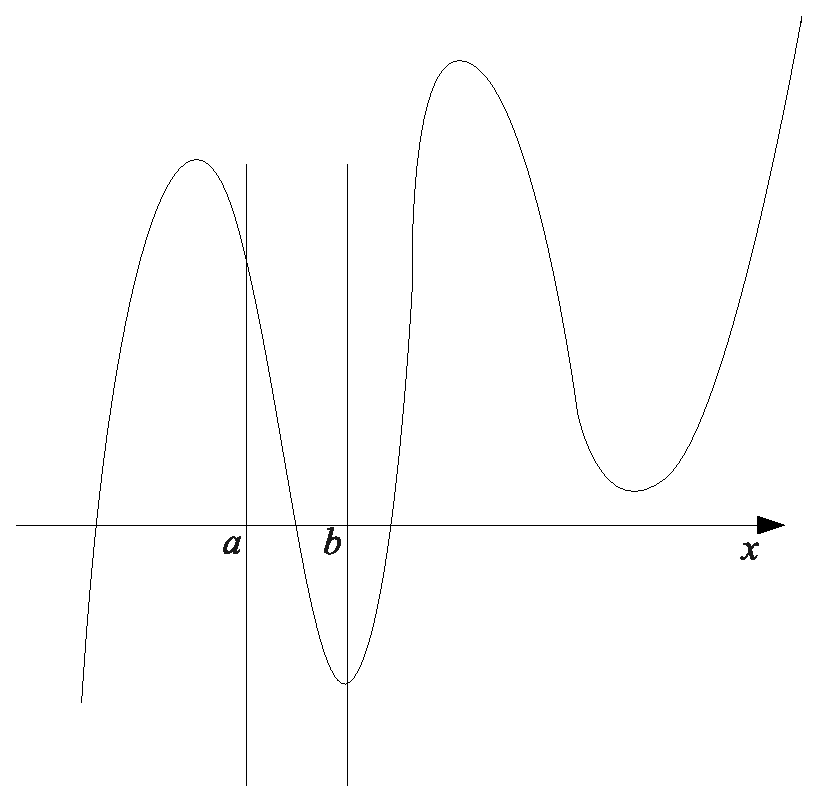
\includegraphics[width=0.5\linewidth,keepaspectratio]{fig15_1.eps}
\caption{方程式$f(x)=0$の様子}\label{fig15_1}
\end{figure}

複数の解を持つ場合は、区間を変えて解く事になる。つまり、このあと考えていくのは「区間内の1つの解を出す」方法である。

\subsection{逐次探索法}
方程式の解の存在がわかっているのであれば、「下手な鉄砲も数撃ちゃ当たる」という方針で、とにかく色々な値を代入してみれば良い。そのうち、方程式を満たす値が見つかるはずである。これを探索する方法の一つが\textbf{逐次探索法}\index{ちくじたんさくほう@逐次探索法}(serial search)である。

区間$[a,b]$の間を幅$h$で見ていく。つまり、$a,a+h,a+2h,\cdots,b$と代入して「解に近いもの」または解を探す。解が直接見つかればもちろんそれで良い。解そのものでなくとも、解の周辺では符号が変わることから、$f(a+kh)\cdot f(a+(k+1)h)<0$となるような場所が見つかるはずである。そこで、この区間$[a+kh,a+(k+1)h]$を、幅$h$をより小さくして再度探索する。これを繰り返していき、望みの精度になったら(小さい正数$\epsilon$に対して、$|f(x')|<\epsilon$となるような$x'$が見つかれば)それを解として出力すれば良い。

これは、解をリニアサーチしているのと同じ事である。計算時間がかかるので、通常はこのアルゴリズムが単独で用いられることはない。

\subsection{二分法}
先のように、解をリニアサーチしても良いのだが、区間が$[a,b]$に定まっていることを利用し、この間をバイナリサーチして解を見つけることもできる。この方法を\textbf{二分法}\index{にぶんほう@二分法}(bisection method)と呼ぶ。但し、$f(a)\cdot f(b)<0$が条件である。以下、手順を示しておく。
\begin{itembox}[l]{二分法}
\begin{enumerate}
\item $f\left(\frac{a+b}{2}\right)$を計算する。これが十分0に近ければ解として終了する。そうでなければ次項に進む。
\item $f(a),f(b)$のうち、先に計算した値と同符号の側の区間を縮める。例えば、$f(b)$が$f\left(\frac{a+b}{2}\right)$と同符号であれば、$b$を$\frac{a+b}{2}$で置き換える。置き換えた後、前項に戻る。
\end{enumerate}
\end{itembox}

\minisec{二分法+逐次探索法}
先に示した方法では$f(a)\cdot f(b)<0$が満たされない時などに使えない。そこで、前準備として逐次探索法を行い、適切な区間を定めてから二分法に切り替えることで高速に解を求めることもできる。
\begin{itembox}[l]{逐次探索付き二分法}
\begin{enumerate}
\item 区間$[a,b]$に対して逐次探索を行い、$f(x')\cdot f(y')<0$となるような$x',y'$を見つける。
\item $f\left(\frac{x'+y'}{2}\right)$を計算する。これが十分0に近ければ解として終了する。そうでなければ次項に進む。
\item $f(x'),f(y')$のうち、先に計算した値と同符号の側の区間を縮め(置き換え)て、前項に戻る。
\end{enumerate}
\end{itembox}

\minisec{二分法/逐次近似法の利用と注意}
ここまでの議論では解が区間$[a,b]$に唯一存在することを仮定しているが、実際にこれがわかっていることは稀だろう。従って、ここまでに紹介した方法はどちらかというと区間$[a,b]$を知る(解を囲い込む)ために用いられる。これらの方法を適用すれば、$f(x)$の符号の変わり目を知ることができ、中間値定理からその解の存在を伺える。

だが、逐次探索法・二分法共に解が充分近い場合はこれらを分離できないことがある。この場合、単純に区間幅を縮めても良いのだが、速度が遅くなり誤差も出やすくなるので、トレードオフとなる。他の方法の場合、これらの近い複数解のうち一つを見つけ出すことができるのに対し、逐次探索法や二分法ではうまくいかないのである。
\\ \\ 
逐次探索法・二分法には更に大きな欠点がある。それは、重解を検知できないことである。$(x-\pi)^2=0$という方程式が重解$\pi$を持つことは直ちにわかるが、この例のように無理数の重解を持つ場合、符号の変わり目がなく、「たまたま調べた場所が0になる」ことも少ないため、解が無いという事になってしまうのである。

その一方、これら2つの方法は急激な変化が起こる関数(例えば、"」"のような形をした関数)に対しても対応するという利点がある。
\\ \\ 
以上のように、方程式の解法は一つに絞るのではなく、様々な種類のものを状況に応じて使い分ける(時に併用する\footnote{実際、Brent法などでは何種類かの方法を状況に応じて戦略的に使い分けている。ソートでも、イントロソートは複数のソートを組み合わせていた。このように、アルゴリズムは状況に応じて適切に選択される必要があるものであり、一つ知っていればそれでいいという事はないのである。})べきなのである。

\subsection{割線法}
\textbf{割線法}\index{わりせんほう@割線法}(secant method)は図\ref{fig15_2}のように、仮の解$x_0,x_1$を定めておき、その2点を通る直線と$x$軸との交点を定め、それを次の「仮の解」$x_2$として、どんどん解を改良していく方法(総称して\textbf{反復法}\index{はんぷくほう@反復法}(iteration method)と呼ばれる)である。

\begin{figure}[htb]
\centering
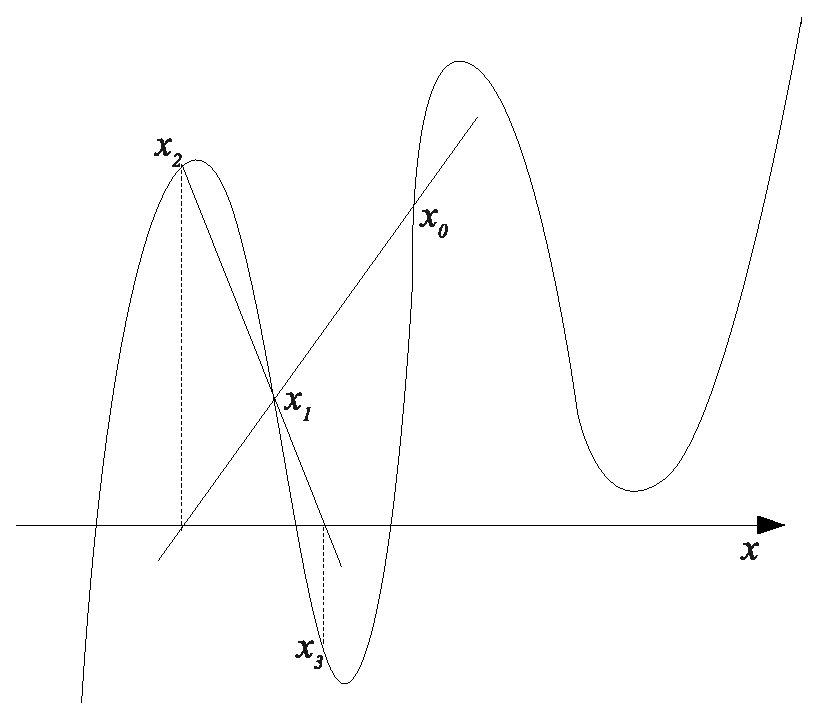
\includegraphics[width=0.5\linewidth,keepaspectratio]{fig15_2.eps}
\caption{割線法の様子}\label{fig15_2}
\end{figure}

\minisec{割線法の漸化式}
図\ref{fig15_2}は人間の目で見れば何をしているか直ちにわかる。だが、コンピュータは図から理解できるわけではないため、何らかの数式で表してやらなければならない。つまり、それまでの仮の解から、次の仮の解を数式によって決定しなければならないのである。以下、この漸化式を導出してみよう。
\\ \\ 
今、2つ前の仮の解が$x_{n-2}$であり、1つ前の仮の解が$x_{n-1}$であったとしよう。この時、この2点を通る直線の方程式は
\begin{equation}
y-f(x_{n-1})=\frac{f(x_{n-1})-f(x_{n-2})}{x_{n-1}-x_{n-2}}(x-x_{n-1})
\end{equation}
である。この直線と$x$軸との交点が$(x_n,0)$なのだから
\begin{equation}
-f(x_{n-1})=\frac{f(x_{n-1})-f(x_{n-2})}{x_{n-1}-x_{n-2}}(x_n-x_{n-1})
\end{equation}
である。これを$x_n$について解いて
\begin{equation}
x_n=x_{n-1}-\frac{x_{n-1}-x_{n-2}}{f(x_{n-1})-f(x_{n-2})}f(x_{n-1}) \label{secant}
\end{equation}
を得る。後は、この漸化式を順次計算すれば良いのである。以下、これを手順化しておく。
\begin{itembox}[l]{割線法}
\begin{enumerate}
\item 仮の解$x_0,x_1$を定める。また、$n=2$とする。
\item 式(\ref{secant})を用いて$x_n$を計算する。
\item 小さい正数$\epsilon$について、$|x_{n}-x_{n-1}|<\epsilon$か、$|f(x_{n})|<\epsilon$が満たされている場合はそれを解として終了する。そうでない場合、$n$を1増やして前項に戻る。
\end{enumerate}
\end{itembox}

\minisec{割線法の利用と注意}
割線法は必ずしも収束するとは限らない他、0に近い極値がある場合、それに影響されやすいという欠点を持つ。しかし、大抵の場合には(初期値さえ適切に選べば)きちんと解を出してくれるので、比較的使いやすい。一度やって収束しなくても、初期値を変えたら収束するような場合もありうるためである。だが、割線法は、複数解がある場合にどれを出すかわからないため、少し厄介である。

ここでは2点からの直線近似としたが、3点からの二次関数近似を利用して解を出す方法もある(Muller法)。Muller法は複素根も求められる優秀な方法であるが、その考えはここで紹介した割線法と原則同じである。そのため、割線法についてまず理解を深め、それから他の書籍などでMuller法を理解されると良いだろう。

\subsection{はさみうち法}
割線法は解を囲い込めないという欠点があった。そこで、囲い込み区間を決定し、その間の解を求められるように割線法を改良したのが\textbf{はさみうち法}\index{はさみうちほう@はさみうち法}あるいは\textbf{レギュラ・ファルシ法}\index{れぎゅらふぁるしほう@レギュラ・ファルシ法|see{はさみうち法}}(regula falsi method)である。
\begin{itembox}[l]{はさみうち法}
\begin{enumerate}
\item 仮の解$a,b$を定める。この時、$f(a)\cdot f(b)<0$を満たすものとする。これから探し求めるのは区間$[a,b]$の実解である。
\item 式(\ref{secant})において、$x_{n-1}=a,x_{n-2}=b$とおいて$x_{n+2}$を計算する。
\item $f(x_{n+2})$が十分0に近ければそれを解として終了する。そうでなければ、二分法同様に、$a,b$のうち符号の同じ側を$x_{n+2}$で置き換え、前項に戻る。
\end{enumerate}
\end{itembox}

はさみうち法は、割線法よりは収束が遅いが、解を囲い込めるのが利点である。初期値によっては二分法よりも遅いが、平均的にはこちらのほうがよく収束する。但し、重解に使えない点は同じである。

\subsection{Newton法}
割線法では2点をとり、それを直線近似することにより解を得た。だが、関数を直線で近似するときには、二点の平均変化率で近似するより各点の接線で近似したほうが正確になるだろう。この考えに基づくアルゴリズムが\textbf{Newton法}\index{Newtonほう@Newton法}ないし\textbf{Newton-Raphson法}と呼ばれるアルゴリズムである。重要なアルゴリズムであるので、まず使い方を述べた後、何種類かの導出を紹介し、その後実例となるソースを一つ見てみることにする。

\minisec{Newton法のアルゴリズム}
Newton法は、割線法と同様に仮の解を定めて、それを改良していく方法である。但し、割線法と違い、接線近似をするために仮の解は一つだけあれば良い。従って、Newton法で解を改良するための漸化式は二項間漸化式であり、次のように与えられる。
\begin{equation}
x_{n}=x_{n-1}-\frac{f(x_{n-1})}{f'(x_{n-1})} \label{Newton}
\end{equation}

この漸化式には何種類かの導出方法があり、後にその内の3種類を示す。先にその手順を示そう(ほとんど割線法と同じである)。

\begin{itembox}[l]{Newton法}
\begin{enumerate}
\item 仮の解$x_0$を定める。$n=1$としておく。
\item 漸化式(\ref{Newton})を用いて$x_n$を計算する。
\item 小さい正数$\epsilon$について、$|x_{n}-x_{n-1}|<\epsilon$か、$|f(x_{n})|<\epsilon$が満たされている場合はそれを解として終了する。そうでない場合、$n$を1増やして前項に戻る。
\end{enumerate}
\end{itembox}

漸化式(\ref{Newton})は収束しない場合がある。例えば、$x_{n+1}=x_{n-1}$となる場合や、極値周辺に落ち込んだ場合などに弱い。従って、ある程度収束の状況を見ておき、適切に収束しない場合は初期値を変えるなどの工夫をしなければならない。幸い、Newton法の収束はここまでに紹介した中でも一番速いので、やり直しても大した手間ではない。

また、関数の極値の大体の位置がわかっているならば、その$x_n$が極値の間から出た時にやり直す、などとすることで収束しやすくできる(上、区間を絞って解を見つけることもできる)。

\minisec{割線法の極限としての導出}
割線法は二点を通る直線によって計算を行う方法であった。この二点を近づけた時に得られる直線が接線になることは先刻承知であろう。従って、割線法の式(\ref{secant})の両辺について$x_{n-2}\rightarrow x_{n-1}$の極限をとった
\begin{equation}
x_n=\lim_{x_{n-2}\rightarrow x_{n-1}} \left(x_{n-1}-\frac{x_{n-1}-x_{n-2}}{f(x_{n-1})-f(x_{n-2})}f(x_{n-1})\right) \label{sec_newton}
\end{equation}
を計算してみる事で、Newton法を導出することができそうである。

ここで、
\begin{equation}
\lim_{x_{n-2}\rightarrow x_{n-1}} \frac{x_{n-1}-x_{n-2}}{f(x_{n-1})-f(x_{n-2})}=\lim_{x_{n-2}\rightarrow x_{n-1}} \frac{1}{\frac{f(x_{n-2})-f(x_{n-1})}{x_{n-2}-x_{n-1}}}=\frac{1}{f'(x_{n-1})}
\end{equation}
である。このことから、式(\ref{sec_newton})は
\begin{equation}
x_n=x_{n-1}-\frac{f(x_{n-1})}{f'(x_{n-1})}
\end{equation}
となり、たしかに式(\ref{Newton})と一致する。
\\ \\ 
以上のように、Newton法は割線法の極限として見ることができる。逆に、微分を差分近似することで割線法に戻すことも可能である(これについては後に述べる)。

\minisec{接線近似からの導出}
先の方法では、平均変化率を求めてから極限を取ることにした。だが、最初から接線を計算すればそれで問題なく導出することができる。釈迦に説法かもしれないが、ここで接線を用いて導出しておこう。

点$(x_{n-1},f(x_{n-1}))$を通る接線の方程式は
\begin{equation}
y-f(x_{n-1})=f'(x_{n-1})(x-x_{n-1})
\end{equation}
である。この接線と$x$軸の交点の$x$座標が$x_n$であるので
\begin{equation}
-f(x_{n-1})=f'(x_{n-1})(x_n-x_{n-1})
\end{equation}
となる。これを解くことで、式(\ref{Newton})が導かれる。
\\ \\ 
先の割線法からの導出は割線法との関係がよく見える方法である。だが、このように接線近似を行ったほうが手早く導出できる。漸化式(\ref{Newton})を忘れた時にはこの方法で導出するのが一番手っ取り早いだろう。

\minisec{解析的導出}
Newton法はTaylor展開を用いた微分近似によっても求められる。この方法は別の解法の導出の際にも用いられるため、ここでNewton法を例にして紹介しておくことにする。

$f(x)$を$x=x_n$でTaylor展開すると
\begin{equation}
f(x)=f(x_n)+f'(x_n)(x-x_n)+\cdots
\end{equation}
となる。この右辺の二次以上の項を落として$f(x)$を一次近似すると
\begin{equation}
f(x)\approx f(x_n)+f'(x_n)(x-x_n)
\end{equation}
となる。ここから、右辺=0の解を求めれば
\begin{equation}
x=x_n-\frac{f(x_{n})}{f'(x_{n})}
\end{equation}
となる。後は、これを順次適用していけば解に近づいていくだろうことから、$x$を$x_{n+1}$で置き換えれば、たしかに式(\ref{Newton})を得られる。

このように、方程式を(必要に応じて近似を行い)変形して左辺と右辺にわけ、右辺を既知項・左辺を未知項として漸化式を導出するのは、反復法において非常によく使われる導出法である。
\\ \\ 
途中、Taylor展開で二次以上を落としたが、二次項まで残すとまた別の解法になる。

\minisec{数値微分との併用}
Newton法の漸化式には、求めたい方程式の導関数がある。導関数が簡単に求まればいいのだが、そうは行かない場合もあるだろう。そこで、コンピュータを用いて数値的に微分を計算(\textbf{数値微分}\index{すうちびぶん@数値微分}(numerical differentiation))してしまえば良いのでは?という考えに至る。

コンピュータで微分を計算する場合、基本となるのは差分近似である。以下、Taylor展開を用いて、1階微分の\textbf{前進差分近似}\index{ぜんしんさぶんきんじ@前進差分近似}(forward difference)と、\textbf{中央差分近似}\index{ちゅうおうさぶんきんじ@中央差分近似}(centered difference)を導出してみよう。

Taylor展開より、十分小さい$h$について、
\begin{equation}
f(x+h)=f(x)+hf'(x)+\cdots \label{taylor}
\end{equation}
である。ここまではどちらの微分近似の導出も同じである。
\\ \\ 
前進差分近似では、式(\ref{taylor})の二次以上の項を落として、$f'(x)$について解く。すると、
\begin{equation}
f'(x)\approx \frac{f(x+h)-f(x)}{h} \label{forward}
\end{equation}
となる。この時の打ち切り誤差は、二次以上の項を落として$h$で割っているので、$O(h)$である。
\\ \\ 
中央差分近似では式(\ref{taylor})を用いて、$f(x+h)-f(x-h)$を計算する。これにより、右辺は奇数次の項しか残らない。
\begin{equation}
f(x+h)-f(x-h)=2hf'(x)+\cdots
\end{equation}
ここで、三次以上の項を落として$f'(x)$についてとけば
\begin{equation}
f'(x)=\frac{f(x+h)-f(x-h)}{2h} \label{centered}
\end{equation}
を得る。この誤差は$O(h^2)$である。
\\ \\ 
今、式(\ref{forward})を用いてNewton法の計算を行うことを考えよう。式(\ref{Newton})に式(\ref{forward})を代入して
\begin{equation}
x_{n}=x_{n-1}-\frac{hf(x_{n-1})}{f(x_{n-1}+h)-f(x_{n-1})}
\end{equation}
を得る。これは、微分を差分化しているので割線法と同様の形式である。つまり、Newton法に前進差分を適用すると割線法に帰着するという事である。これは何も前進差分に限った話ではない。中央差分近似を始めとする他の方法を使ったとしても、割線法と本質的には同じアルゴリズムになる(平均変化率の計算が少し変わるだけ)。

ここで述べた方法によりNewton法に数値微分を組み合わせた場合、割線法を(任意の幅で)用いる場合に比べて収束が遅い場合が多い為、これを使うぐらいなら最初から割線法で攻めたほうが良いだろう。しかし、割線法とNewton法の関係が、差分と微分の関係であることを理解するのに重要なことであるため、ここで述べた。
\\ \\ 
なお、蛇足ながら、数値微分の差分近似方法はここに紹介した以外にも沢山あり、Taylor展開から導出できる。例えば、$f(x+h)+f(x-h)$から二階微分の公式が導出できる他、$f(x),f(x\pm h),f(x\pm 2h)$を用いて一階微分を計算することにより、より精度の良い公式が導出できる。興味があれば計算してみていただきたい。

\minisec{Newton法の実例〜平方根の計算〜}
ここまでで、Newton法の素性について学習したので、これを実際に使って正平方根を計算する関数を作成してみることにしよう。
\\ \\ 
ソースコードの前に、Newton法の漸化式をどう書けばいいか考えておく。数$a$の正平方根$\sqrt{a}$を解に持つ方程式のうち、$x$と$a$及び定数だけで簡単に書けるものとして
\begin{equation}
x^2-a=0
\end{equation}
という方程式が挙げられる。これをNewton法により解く。

$f(x)=x^2-a$として、式(\ref{Newton})を書き下すと
\begin{equation}
x_{n}=x_{n-1}-\frac{x_{n-1}^2-a}{2x_{n-1}}
\end{equation}
である。初期値は、正の値ならば(その形状を推測して)何でも良いが、ここでは決めやすく$a$としておこう。これにより、Newton法を書く準備ができたので、以下に引数の正平方根を計算する関数を実装してみることにする。
\begin{boxnote}
\begin{multicols}{2}
\minisec{Newton法による平方根の計算}
Newton法を用いて引数の正の平方根を計算する関数\verb|newton_sqrt|を実装してみる。ここでは、収束の判定を、解候補の二乗と元の数の差が$10^{-6}$未満であるとし、マクロ\verb|EPS|によって定めるものとした。なお、収束しない場合の処理などは行なっていない。
\begin{lstlisting}[caption=Newton法による開平,label=program15_1]
#include<math.h>
#define EPS 1E-6

double newton_sqrt(double a){
  double x=a;
  do{
    x-=(x*x-a)/(2*x);
  }while(fabs(x*x-a)>=EPS);
  return x;
}
\end{lstlisting}
\end{multicols}
\end{boxnote}

このように、解を求めることができる方程式に対しても、その解の数値の計算のためなどの理由で、数値解法を用いる場合があるのである。

\section{数値積分法}
ある定積分を数値的に計算する。積分は面積であるから、その面積を何らかの近似で求められれば良い。この時、区間を大きく取ると近似しづらくなるので、
\begin{equation}
\int^{b}_{a} f(x)=\sum^{n-1}_{k=0}\int^{x_{k+1}}_{x_k}f(x)dx \ \quad(x_0=a,x_n=b) \label{integrals}
\end{equation}
のように区間に分割して計算を行う。数列$\{x_n\}$を$x_{n+1}=x_n+h$として決めれば、これは等分割になることがわかるだろう。ここでは、このような等分割の場合\footnote{ガウス・ルジャンドルの積分公式など等分割にしない方法も存在する。}に、右辺の積分をどのように近似するかを見ていくことにする。最後に、少し違ったアプローチでの積分方法を紹介する。

\subsection{台形則}
以前の講義で既に紹介したが、\textbf{台形則}\index{だいけいそく@台形則|see{台形積分}}ないし\textbf{台形積分}\index{だいけいせきぶん@台形積分}公式は、式(\ref{integrals})右辺の積分を台形によって近似し
\begin{equation}
\int^{x_{k+1}}_{x_k}f(x)dx=\int^{x_k+h}_{x_k}f(x)dx\approx \frac{h}{2}\left(f(x_k)+f(x_k+h)\right)
\end{equation}
と近似する方法である。

\subsection{中点則}
\textbf{中点則}\index{ちゅうてんそく@中点則}(midpoint integral)は、区間分割の近似を台形ではなく長方形で行う方法である。この時、長方形の幅が$h$であることはすぐにわかるが、高さには幾つかの選び方がある。$f(x_k)$や$f(x_k+h)$を高さにする方法は高校などで区分求積法として説明されるが、中点則ではその名前通り、中点を高さにとる。つまり、$f(x+0.5h)$を高さの基準として用いる。これにより、式(\ref{integrals})右辺の積分は
\begin{equation}
\int^{x_{k+1}}_{x_k}f(x)dx=\int^{x_k+h}_{x_k}f(x)dx\approx hf(x_k+0.5h)
\end{equation}
と簡単に近似できる。
\\ \\ 
通常、数値積分では台形則の方がよく用いられるが、このような方法があることも知っておくと良い。

\subsection{シンプソン則}
\textbf{シンプソン則}\index{しんぷそんそく@シンプソン則}(Simpson integral)は古典的な積分公式として知られている方法である。台形則よりも時間がかかるため精度が必要ない場合には使われず、精度が必要な場合はローンバーグ積分やガウス・ルジャンドル積分の方が有用であるのでやはり使われないという、博物館行きになった感のある公式である。とはいえ、初歩として知っておく価値はあるので、ここでその概要を紹介しておこう。

$x_k,x_k+0.5h,x_k+h$から、関数を二次関数で近似することを考える。ただし、この形式で書くのは面倒であるので、$x'_-=x_k,x'=x_k+0.5h,x'_+=x_k+h$および$h'=0.5h$とおいて議論を進める(こちらのほうが一般的な形になるため)。また、$f'_-=f(x'_-),f'_+=f(x'_+),f'=f(x')$とする。
\\ \\ 
三点を通る二次関数$g(x)$は唯一に定まる。そこで、(簡単のため)二次関数を
\begin{equation}
g(x)=a(x-x')^2+b(x-x')+c
\end{equation}
とおき、これが3点を通るように$a,b,c$を定めることとする。単純に各点を代入して解けば
\begin{equation}
\left(a,b,c\right)=\left(\frac{f'_-+f'_+-2f'}{2h'^2},\frac{f'_+-f'_-}{2h'},f'\right) \label{simpson1}
\end{equation}
となる。一方、
\begin{equation}
\int g(x)dx=\frac{a}{3}(x-x')^3+\frac{b}{2}(x-x')^2+cx \label{simpson2}
\end{equation}
である(ただし、積分定数を省いた)。

式(\ref{simpson2})に式(\ref{simpson1})を代入して整理し、定積分の形に書き直すと
\begin{equation}
\int^{x'_+}_{x'_-}f(x)dx\approx \int^{x'_+}_{x'_-}g(x)dx=\frac{h'}{3}[f'_-+4f'+f'_+]
\end{equation}
を得る。これが、シンプソン則である。
\\ \\ 
シンプソン則を用いる場合は、先のように中点を用いる場合もあるし、3点ずつ適用するように変える方法もある。

\subsection{モンテカルロ積分}
\textbf{モンテカルロ積分}\index{もんてかるろせきぶん@モンテカルロ積分}(Monte Carlo integral)は、ここまでの方法とは変わった形で積分を行う方法で、とりわけ多次元積分や解析的に書きにくい領域の面積を求めるのに用いられる。なお、一般のアルゴリズムで\textbf{モンテカルロ法}\index{もんてかるろほう@モンテカルロ法}(Monte Carlo method)と言った場合、乱数を用いて計算を行うアルゴリズムで、それ故に結果が正しいとは限らないもののことを言う\footnote{これに対し、乱択クイックソートのように、乱数を使うがゆえに時間が一定に定まらない(解は正しく出る)ものを\textbf{ラスベガス法}\index{らすべがすほう@ラスベガス法}(Las Vegas method)と呼ぶ。}。ここで挙げたモンテカルロ積分もモンテカルロ法の一種である。
\\ \\ 
積分したい領域を図\ref{monte}のように長方形で囲む。そして、囲んだ領域に対し、一様乱数を用いて\footnote{これがどの程度一様か、と言う所で正確性が定まる。計算向けにはC言語の標準関数のrandを用いるよりも、メルセンヌ・ツイスターと呼ばれる方法を用いたほうが良い。}点を「撒く」。そして、このうち幾つの点が領域内に入っているか、その割合を出せば囲んだ領域の近似となるだろう。
\begin{figure}[htb]
\centering
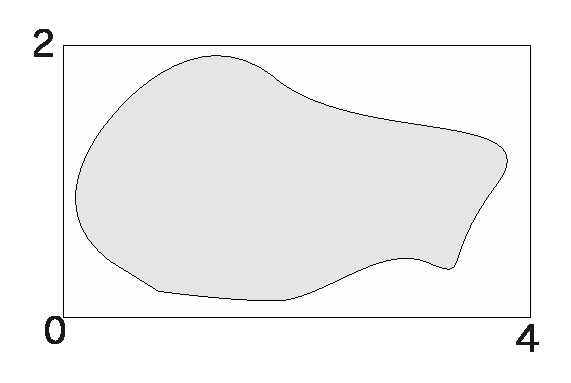
\includegraphics[width=0.6\linewidth,keepaspectratio]{fig15_3.eps}
\caption{モンテカルロ積分したい領域の様子(灰色領域)}\label{monte}
\end{figure}

この近似方法を手順にしてまとめておこう。
\begin{itembox}[l]{二次元のモンテカルロ積分}
\begin{enumerate}
\item 計算したい領域を長方形で囲む。また、$c=0$とする。
\item 次の2つの操作を$n$(任意の自然数値)回繰り返す。
\begin{enumerate}[(1)]
\item 長方形内の点を一点、一様乱数を用いて選ぶ。
\item 選んだ点が積分領域内に入っているかどうかを判定し、入っている場合は$c$を1増やす。
\end{enumerate}
\item 長方形の面積$\times c/n$を計算し、それを積分値とする。
\end{enumerate}
\end{itembox}

この方法は、3次元の場合でも長方形を直方体に変えるだけで実行できるので、多次元積分に使いやすい。また、積分領域が解析的に書き表しにくい場合でも、領域として判定できさえすればいいので、台形積分が使えない場合などでも使えるという利点がある。
\\ \\ 
モンテカルロ積分の精度は、$n$が十分大きいならば、寧ろ一様性による。つまり$n=2^{16}$であるのを$n=2^{20}$に増やすよりも、乱数がより一ように出るようにしたほうが精度が良くなる。十分良い規則があるならば、点を選ぶのに乱数を用いず、規則性を用いて一様性を確保することもできる(\textbf{準モンテカルロ積分}\index{じゅんもんてかるろせきぶん@準モンテカルロ積分}(semi-Monte Carlo integral)と呼ぶ)。だが、例えば細かい波状の境界の場合などは、適切な規則性が見当たらず、乱数を用いて選んだほうが適切に点を選べる場合もある。

\section{連立方程式と行列}
多元一次連立方程式を解く際に行列を用いる方法については既知であろう。この行基本変形をシステマティックに行うことによって、数値的に連立方程式の解を得ることができる。連立方程式を解くことは、数値計算の各所で必要になる操作であるため、ここでその基本を紹介しておく。また、その簡単な応用として、逆行列や行列式を求める方法についても触れる。なお、ここで紹介する方法についてのライブラリを作成するのは、配列・構造体・ポインタなどの良い復習になるので、できれば汎用ライブラリとしてまとめてみると良い。
\subsection{Gauss法}
\textbf{Gauss法}\index{Gaussほう@Gauss法}(Gaussian Elimination)は、連立方程式を解く方法では最もポピュラーな方法であり、前進消去過程と後退代入過程からなる。

\minisec{前進消去過程}
連立方程式を表すため、以下、$n$行$n+1$列からなる拡大係数行列$A$を考える。もちろん、第$n+1$列は連立方程式の定数ベクトルである。また、$a_{i,j}$と書いた場合、これは行列$A$の$i,j$成分を指すものとする。
\\ \\ 
拡大係数行列の下三角成分を0にする過程が前進消去過程である。前進消去過程では、第$k$行を用いて第$k+1$行以降の各行の第$k$列成分を0にする。これを$k=1$から順にやることで、下三角成分を0にすることができる。手順をまとめておこう。
\begin{itembox}[l]{Gauss法の前進消去過程}
\begin{enumerate}
\item $k=1$としておく。
\item $i=k+1,k+2,\cdots$及び$j=k+1,k+2,\cdots$として、次の計算を行う(ただし、$-=$はC言語の\verb|-=|と同じ意味)。
\begin{equation}
a_{i,j}-=\frac{a_{i,k}}{a_{k,k}}a_{k,j} \label{gauss1}
\end{equation}
\item $k=n$であれば終了する。そうでなければ、$k$を1増やし、前項に戻る。
\end{enumerate}
\end{itembox}

なお、実際の計算では、下三角が0になることはわかっているので、影響がある上三角部分だけ計算するようにしている。

以上により前進消去過程が行われたら、続いて後退代入過程を施し、連立方程式を解く。

\minisec{後退代入過程}
前進消去が行われた状態では、一番下(第$n$行)は単なる一次方程式になっている。そこで、これを解くことで、解のうちの一つを求めることができる。求めた解を、一つ上(第$n-1$行)に代入して計算すれば、解成分がもうひとつ明らかになる。このように、下側から代入して解を求める…を繰り返すことで、連立方程式の解を求めることができる。これが、後退代入過程である。
\begin{itembox}[l]{Gauss法の後退代入過程}
\begin{enumerate}
\item $k=n$としておく。また、$x_i$は解ベクトルの第$i$成分とする。
\item 次の式により、$x_k$を求める(ただし、$k=n$の時には総和部分は計算されない)。
\begin{equation}
x_k=\frac{1}{a_{k,k}}\left(a_{k,n+1}-\sum^{n}_{i=k+1}a_{k,i}x_{i}\right) \label{gauss2}
\end{equation}
\item $k=1$であれば終了する。そうでなければ、$k$を1減らし、前項に戻る。
\end{enumerate}
\end{itembox}

なお、この方法を用いるときに、総和を逐次求めるのではなく、$x_k$がわかった時にそこから上の行について減算を行なっておくという実装もできる。
\\ \\ 
実際には、ここまでに述べた前進消去と後退代入をあわせてGauss法と呼んでおり、これらは一連の作業である。だが、分けたほうがこのあとの説明に便利であるため、2つに分けて説明した。

\minisec{部分ピボット選択}
前進消去過程の式(\ref{gauss1})においては、割り算を伴うため、0による除算をしないように気をつけなければならない。だが、計算過程において$a_{k,k}$が0になってしまう場合は十分にありうる。こんな時に行うのが\textbf{ピボット選択}\index{ぴぼっとせんたく@(連立方程式の)ピボット選択}(pivot selection)である。ここで、ピボットというのは$a_{k,k}$のように、行/列とも同じ番号の成分のことを言う。

もしもピボット$a_{k,k}$が0になってしまった場合(あるいは絶対値が非常に小さい場合)、そこから下の行を見ていき、0でない成分$a_{j,k}$($j>k$)を探し求める。適切な$j$が見つかったら、第$k$行と第$j$行を入れ替える\footnote{蛇足ながら、浅いコピーを用いたほうが速度が速くて良い。}。このような行交換を行う方法が\textbf{部分ピボット選択}である。なお、行交換に加えて列交換も行う\textbf{完全ピボット選択}もあるのだが、ここでは名前だけの紹介に留める。
\\ \\ 
部分ピボット選択は、0による除算の回避のためだけにあるのではない。実際は、小さい値による割り算を行うと誤差が出たりする場合があるため、それを緩和する役目も持っている。一般には、同じ列の成分のうち、最も絶対値の大きい値をピボットに持ってくると良いとされる。これを含めて、前進消去過程を書き換えよう。
\begin{itembox}[l]{部分ピボット選択付き前進消去}
\begin{enumerate}
\item $k=1$としておく。
\item $a_{i,k}\ (i\ge k)$のうち、絶対値が最も大きい値を求める($a_{m,k}$とする)。求めた$m$に対し、$m$行と$k$行を交換する。
\item $i=k+1,k+2,\cdots$及び$j=k+1,k+2,\cdots$として、式(\ref{gauss1})の計算を行う。
\item $k=n$であれば終了する。そうでなければ、$k$を1増やし、前々項に戻る。
\end{enumerate}
\end{itembox}

なお、部分ピボット選択の過程において、ある列で0の要素しか見当たらなくなった場合、その連立方程式には解が存在しないか、解が無数にある。この判定ができることも含めて、連立方程式を解く際には部分ピボット選択をつけておくと良い。

\minisec{LU分解}
同じ係数行列でありながら、定ベクトルが異なる複数の連立方程式を解くことがある。このような場合に高速化を図る手法が\textbf{LU分解}\index{LUぶんかい@LU分解}(LU decomposition)である。ここでは、数学的な議論は割愛し、プログラミングの観点からLU分解を扱う。
\\ \\ 
同じ係数行列・異なる定ベクトルであれば、前進消去過程の大半(定ベクトルに対する計算以外の部分)は無駄である。従って、何とかしてこの無駄な部分を省くことはできないか、と考えてみる。

定ベクトルの計算に必要なのは、消去の時に、その行を何倍して引いたかという情報だけである。つまり、各過程における$\frac{a_{i,k}}{a_{k,k}}$さえわかれば、後は定ベクトルを計算することができる。従って、$\frac{a_{i,k}}{a_{k,k}}$を記録しておこう、という事になる。この時、行列の下三角成分は無益に残っているだけなので、そこにメモすれば良い。これを手順化すると、次のようになる。
\begin{itembox}[l]{行列のLU分解}
以下、拡大係数行列ではなく、$n\times n$の係数行列を考えるものとする(ピボット選択は省いたが、省かずとも同じ手順である)。
\begin{enumerate}
\item $k=1$としておく。
\item $i=k+1,k+2,\cdots$及び$j=k+1,k+2,\cdots$として、式(\ref{gauss1})の計算を行う。更に、この時の$\frac{a_{i,k}}{a_{k,k}}$の値を$a_{i,k}$に保存しておく。
\item $k=n$であれば終了する。そうでなければ、$k$を1増やし、前項に戻る。
\end{enumerate}
\end{itembox}

一度上記の手順を踏んで計算すれば、後は次の手順で(異なる定ベクトルに対しても)解を求められる。
\begin{itembox}[l]{LU分解後の解の計算}
以下、定ベクトルの第$i$成分を$b_i$と記す。
\begin{enumerate}
\item $k=1$としておく。
\item $i=k+1,k+2,\cdots$とし、$b_i$から$a_{i,k}\cdot b_k$を引く。
\item $k=n$ならば次項へ進む。そうでなければ$k$を1増やして前項に戻る。
\item 後退代入過程を行い、解を計算する。
\end{enumerate}
\end{itembox}

「その方程式を解くのは一度限り!」という場合を除いては、この方法により計算すれば同じ計算を省略することが出来る。

\subsection{Gauss-Jordan法}
\textbf{Gauss-Jordan法}\index{Gauss-Jordanほう@Gauss-Jordan法}はGauss法よりも少し遅いが、間違えづらい方法で、特に逆行列への応用が効きやすい方法である。なお、ここでもやはり拡大係数行列を用いて説明を行う。
\\ \\ 
Gauss-Jordan法は、係数行列に行基本変形を行い、単位行列に変換することによって連立方程式を解く方法である。早速手順を見てみよう(部分ピボット選択を含んでいる)。
\begin{itembox}[l]{Gauss-Jordan法}
\begin{enumerate}
\item $k=1$としておく。
\item $a_{k,k}$が0である場合、$a_{i,k}\neq0\ (i>k)$を満たす行を見つけ、第$i$行と第$k$行を交換する。
\item 第$k$行の全ての成分を$a_{k,k}$で割っておく。これにより、$a_{k,k}=1$となる。
\item $i\neq k$なる全ての$i$に対し、第$i$行から($a_{i,k}\times$第$k$行)を引く。
\item $k=n$ならば終了する。そうでなければ$k$を1増やし、ステップ2に戻る。
\end{enumerate}
\end{itembox}

この変形により、係数行列は単位行列になり、定ベクトル(拡大係数行列の第$n+1$列)は解ベクトルそのものになっている。
\\ \\ 
この方法はGauss法に比べて実装が楽なので、しばしば、連立方程式の解を出すアルゴリズムの試験のために用いられる。

\subsection{行列式や逆行列への応用}
Gauss法やGauss-Jordan法は行基本変形を元にしているため、他の行列操作にも応用できる。ここでは、Gauss法を行列式に、Gauss-Jordan法を逆行列に応用してみよう。

\minisec{Gauss法による行列式の計算}
行列式の計算を行う場合、第1列の成分のうち第1行以外を0にすれば、これが定数となって出てくる。すなわち、
\begin{equation}
\left|
\begin{array}{ccc}
a_{1,1}&\cdots&a_{1,n}\\
0&\cdots&a_{2,n}\\
\vdots&\ddots&\vdots\\
0&\cdots&a_{n,n}
\end{array}
\right|=a_{1,1}\left|
\begin{array}{ccc}
a_{2,2}&\cdots&a_{2,n}\\
\vdots&\ddots&\vdots\\
a_{n,2}&\cdots&a_{n,n}
\end{array}
\right|
\end{equation}
とできる。ここで、$a_{k,k}$を用いてそこから下の成分を0にするのは、Gauss法の前進消去過程そのものであることを思い出せば、前進消去の際にピボットを随時掛け算していくことによって行列式の値を計算することができることがわかるだろう。

\minisec{Gauss-Jordan法による逆行列の計算}
係数行列と単位行列をくっつけた
\begin{equation}
\left[
\begin{array}{ccc|ccc}
a_{1,1}&\cdots&a_{1,n}&1&\cdots&0\\
\vdots&\ddots&\vdots&\vdots&\ddots&\vdots\\
a_{n,1}&\cdots&a_{n,n}&0&\cdots&1
\end{array}\right]
\end{equation}
を用意し、これに対してGauss-Jordan法を適用すると逆行列を得ることができる。これは、Gauss法でも同じ事である。特段説明することはないだろう。
\\ \\ 
注意すべき点として、この方法で逆行列を求めてから連立方程式を解くと、速度が遅く、誤差も大きくなりがちである。これは、連立方程式に限ったことではない。例えば、$x_{k+1}=A^{-1}x_k$のような漸化式がある場合、$Ax_{k+1}=x_k$と変形してLU分解を用いたほうが逆行列を計算するよりも(特に誤差の面で)良い結果が得られる。従って、この方法で逆行列を得るのは、あくまでも逆行列そのものに興味がある場合と考えて良い。
\\ \\ 
実は、この方法は逆行列を得る方法としても最適のものではない。実際には、「第$i$成分が1で他は0」という解ベクトルを$i=1,\cdots,n$として用意し、LU分解を用いて解いたほうが良い。実際に計算回数を見積もってみていただきたい。

\newpage

\begin{shadebox}
\section*{本講の要点}
本講では、分野を問わずよく使われるであろう基礎的な数値計算法を学んだ。

\subsection*{一元方程式の解法}
\begin{itemize}
\item 代数方程式の解を数値的に出す場合、一度に全ての解を出すことは通常難しいため、区間を絞って一つずつ出していくことになる。
\item 区間をリニアサーチするのが逐次探索法、二分探索するのが二分法である。
\item 割線法は曲線上の2点をとり、それらを結ぶ直線を引いて$x$軸との交点を求めるという操作を繰り返すことで解を求める方法である。
\item 割線法に、二分法と似たような区間制限をつけたのがはさみうち法である。
\item 割線法の極限として、接線を用いて近似したのがNewton法である。
\end{itemize}

\subsection*{数値積分法}
\begin{itemize}
\item 数値積分を行う場合は通常、小区間に分割し、その各区間を近似的に計算して総和を求める形で積分する。
\item 台形則は台形・中点則は中点の高さの長方形で区間を近似する。
\item シンプソン則は関数上に3点をとり、そこを二次関数近似することによって積分を計算する。
\item モンテカルロ積分は、領域の面積を求めるのに適した方法で、点を「撒いて」、それが求めたい領域に入った割合によって計算する方法である。
\end{itemize}

\subsection*{連立方程式と行列}
\begin{itemize}
\item Gauss法は下三角成分を0にする前進消去過程と、それによって解を順次求めていく後退代入過程からなる。
\item Gauss-Jordan法は係数行列を単位行列に変換することによって解を求める方法である。
\item 同じ係数行列に対して前進消去過程を繰り返すのは無意味であるので、それをメモしておいて複数の定ベクトルに使いまわす方法がLU分解である。
\item 行基本変形のうち、行交換の過程のことを部分ピボット選択と呼んでいる。
\item 連立方程式を解くアルゴリズムは、逆行列や行列式の値を求める際に容易に応用できる。
\end{itemize}

\end{shadebox}


\beginappendix
\chapter{簡易リファレンス}
C言語の簡易リファレンスを掲載しておく。紙面の都合上、記述は最小限度にとどめたので、利用方法についてはmanコマンドはじめインターネット等で調べて頂きたい。なお、以下の書籍・サイトを参考にした。
\begin{itemize}
\item C言語によるプログラミング[応用編]第2版(内田他著、Ohm社刊)
\item C言語によるプログラミング[スーパーリファレンス編](内田他著、Ohm社刊)
\item C言語プログラミング(H.M.Deitel他著、ピアソン・エデュケーション刊)
\item プログラミング言語C 第2版 (B.W.Kernighan他著、共立出版刊)
\item Cリファレンスマニュアル第5版(S.P.Harbison他著、SiB access刊)(C99)
\item プログラミング言語Cの新機能(\verb|http://seclan.dll.jp/c99d/|)(C99)
\item C言語関数辞典(\verb|http://www.c-tipsref.com/|)(C99)
\end{itemize}
なお、末尾にC99と付したものはC95,C99で追加された機能について用いたものである。\\

特に断らない限り、大文字で書いているものはマクロであり、型・引数を書いているものは関数である。なお、ヘッダ内で返却値の型や引数の取り方が同じである関数については冒頭にそれを断った上で関数名のみを記している(ctype.hやmath.hなど)。また、便宜上、C89の部分とC95/C99の部分は分けて書き、C95/C99で追加された関数やヘッダはC89の後に追加した。

\section{assert.h(プログラム診断)}
\begin{itemize}
\item \verb|NDEBUG|:定義することで\verb|assert()|を無効にする。
\item \verb|void assert(int expression)|:実行時の条件チェック。\verb|expression|が偽の際にファイル名と行番号を\verb|stderr|に出力して\verb|abort|する。
\end{itemize}
 
\section{ctype.h(文字の分類)}
本ヘッダで定義される関数はいずれも\verb|int function(int argument)|の形である。以下、関数名のみ記している。また、主語「引数が」を省略している。
\begin{itemize}
\begin{multicols}{2}
\item \verb|isalnum|:半角英数字ならば真。
\item \verb|isalpha|:アルファベットならば真。
\item \verb|islower|:英小文字ならば真。
\item \verb|isupper|:英大文字ならば真。
\item \verb|isdigit|:数字ならば真。
\item \verb|isxdigit|:16進数ならば真。
\item \verb|iscntrl|:制御文字ならば真。
\item \verb|ispunct|:区切り文字ならば真。
\item \verb|isspace|:空白文字ならば真。
\end{multicols}
\item \verb|isgraph|:スペース以外の印字可能文字ならば真。
\item \verb|isprint|:スペースを含む印字可能文字ならば真。
\item \verb|tolower|:英大文字であるならば対応する英小文字を返し、それ以外の場合は引数の値を返す。
\item \verb|toupper|:英小文字であるならば対応する英大文字を返し、それ以外の場合は引数の値を返す。
\end{itemize}
以下は、C99において追加された関数である。
\begin{itemize}
\item \verb|isblank|:行中空白ならば真。
\end{itemize}

\section{errno.h(エラー)}
\begin{itemize}
\begin{multicols}{2}
\item \verb|EDOM|:定義域エラー
\item \verb|ERANGE|:値域エラー
\end{multicols}
\item \verb|errno|:エラー状態を保持する外部変数
\end{itemize}

\section{float.h(浮動小数点数型属性検査)}
いずれも環境依存のマクロである。
\begin{itemize}
\item \verb|DBL_DIG|:\verb|double|型変数が10進数で表すことのできる精度の桁数
\item \verb|DBL_EPSILON|:\verb|double|型変数でのマシンイプシロンの値
\item \verb|DBL_MANT_DIG|:\verb|double|型変数の仮数部における基数\verb|FLT_RADIX|の桁数
\item \verb|DBL_MAX|:\verb|double|型変数の表現可能な最大値
\item \verb|DBL_MAX_10_EXP|:\verb|double|型変数の表現可能な指数最大値(基数10)
\item \verb|DBL_MAX_EXP|:\verb|double|型変数の表現可能な指数最大値(基数2)
\item \verb|DBL_MIN|:\verb|double|型変数の表現可能な正の最小値
\item \verb|DBL_MIN_10_EXP|:\verb|double|型変数の表現可能な指数最小値(基数10)
\item \verb|DBL_MIN_EXP|:\verb|double|型変数の表現可能な指数最小値(基数2)
\item \verb|DBL_ROUNDS|:\verb|double|型変数の足し算に対する丸めモード
\item \verb|FLT_DIG|:\verb|float|型変数が10進数で表すことのできる精度の桁数
\item \verb|FLT_EPSILON|:\verb|float|型変数でのマシンイプシロンの値
\item \verb|FLT_MANT_DIG|:\verb|float|型変数の仮数部における基数\verb|FLT_RADIX|の桁数
\item \verb|FLT_MAX|:\verb|float|型変数の表現可能な最大値
\item \verb|FLT_MAX_10_EXP|:\verb|float|型変数の表現可能な指数最大値(基数10)
\item \verb|FLT_MAX_EXP|:\verb|float|型変数の表現可能な指数最大値(基数2)
\item \verb|FLT_MIN|:\verb|float|型変数の表現可能な正の最小値
\item \verb|FLT_MIN_10_EXP|:\verb|float|型変数の表現可能な指数最小値(基数10)
\item \verb|FLT_MIN_EXP|:\verb|float|型変数の表現可能な指数最小値(基数2)
\item \verb|FLT_RADIX|:\verb|float|型変数の指数表現の基数
\item \verb|FLT_ROUNDS|:\verb|float|型変数の足し算に対する丸めモード
\item \verb|LDBL_DIG|:\verb|long double|型変数が10進数で表すことのできる精度の桁数
\item \verb|LDBL_EPSILON|:\verb|long double|型変数でのマシンイプシロンの値
\item \verb|LDBL_MANT_DIG|:\verb|long double|型変数の仮数部における基数\verb|FLT_RADIX|の桁数
\item \verb|LDBL_MAX|:\verb|long double|型変数の表現可能な最大値
\item \verb|LDBL_MAX_10_EXP|:\verb|long double|型変数の表現可能な指数最大値(基数10)
\item \verb|LDBL_MAX_EXP|:\verb|long double|型変数の表現可能な指数最大値(基数2)
\item \verb|LDBL_MIN|:\verb|long double|型変数の表現可能な正の最小値
\item \verb|LDBL_MIN_10_EXP|:\verb|long double|型変数の表現可能な指数最小値(基数10)
\item \verb|LDBL_MIN_EXP|:\verb|long double|型変数の表現可能な指数最小値(基数2)
\item \verb|LDBL_ROUNDS|:\verb|long double|型変数の足し算に対する丸めモード
\end{itemize}
以下はC99において追加されたマクロである。
\begin{itemize}
\item \verb|DECIMAL_DIG|:|:浮動小数点数型で表現できる最大の10進桁数
\item \verb|FLT_EVAL_METHOD|:実際に浮動小数点数演算を行うときの範囲と精度を示す値
\end{itemize}

\section{limits.h(整数型属性検査)}
いずれも環境依存のマクロである。
\begin{itemize}
\item \verb|CHAR_BIT|:\verb|char|型変数のビット数
\item \verb|CHAR_MAX|:\verb|char|型変数の表現可能な最大値
\item \verb|CHAR_MIN|:\verb|char|型変数の表現可能な最小値
\item \verb|INT_MAX|:\verb|int|型変数の表現可能な最大値
\item \verb|INT_MIN|:\verb|int|型変数の表現可能な最小値
\item \verb|LONG_MAX|:\verb|long|型変数の表現可能な最大値
\item \verb|LONG_MIN|:\verb|long|型変数の表現可能な最小値
\item \verb|MB_LEN_MAX|:多バイト文字の最大バイト数
\item \verb|SCHAR_MAX|:\verb|signed char|型変数の表現可能な最大値
\item \verb|SCHAR_MIN|:\verb|signed char|型変数の表現可能な最小値
\item \verb|SHRT_MAX|:\verb|short|型変数の表現可能な最大値
\item \verb|SHRT_MIN|:\verb|short|型変数の表現可能な最小値
\item \verb|UCHAR_MAX|:\verb|unsigned char|型変数の表現可能な最大値
\item \verb|UINT_MAX|:\verb|unsigned int|型変数の表現可能な最大値
\item \verb|ULONG_MAX|:\verb|unsigned long|型変数の表現可能な最大値
\item \verb|USHRT_MAX|:\verb|unsigned short|型変数の表現可能な最大値
\end{itemize}
以下は、C99において追加されたマクロである。
\begin{itemize}
\item \verb|LLONG_MAX|:\verb|long long|型変数の表現可能な最大値
\item \verb|LLONG_MIN|:\verb|long long|型変数の表現可能な最小値
\item \verb|ULLONG_MAX|:\verb|unsigned long long|型変数の表現可能な最大値
\end{itemize}

\section{locale.h(地域情報管理)}
\begin{itemize}
\item \verb|LC_ALL|:全ての地域情報に対する検索・設定用定数
\item \verb|LC_COLLATE|:地域固有の文字の比較順序情報に対する検索・設定用定数
\item \verb|LC_CTYPE|:地域固有文字(多バイト文字等)に対する検索・設定用定数
\item \verb|LC_MONETARY|:地域固有の通貨文字に対する検索・設定用定数
\item \verb|LC_NUMERIC|:地域固有の小数点文字に対する検索・設定用定数
\item \verb|LC_TIME|:地域固有の時間表現文字列に対する検索・設定用定数
\item \verb|NULL|:\verb|NULL|ポインタ
\item \verb|struct lconv|:地域固有の表現情報を格納する構造体
\item \verb|char *setlocale(int category,const char *locale)|:地域情報を設定する。\\ \verb|locale|が\verb|NULL|の時は地域情報を検索する。
\item \verb|struct lconv *localeconv(void)|:地域情報が格納された構造体\verb|lconv|へのポインタを返す。
\end{itemize}

\section{math.h(数学関数)}
gccでコンパイルする際には\verb|-lm|オプションをつけ\verb|gcc source.c -lm|とする必要がある。

以下特に断らない限り、型が省略されたものを\verb|double|型とする。
\begin{itemize}
\item \verb|HUGE_VAL|:\verb|double|型変数の表現可能な最大値(パソコンにおける「十分大きい値」)。C99ではこれにF,Lをつけたものもある。
\begin{multicols}{2}
\item \verb|acos(x)|:逆余弦を返す。$\cos^{-1}(x)$
\item \verb|asin(x)|:逆正弦を返す。$\sin^{-1}(x)$
\item \verb|atan(x)|:逆正接を返す。$\tan^{-1}(x)$
\item \verb|atan2(y,x)|:点$(x,y)$の方向角を返す。$\tan^{-1}(y/x)$。
\item \verb|cos(x)|:余弦を返す。$\cos x$
\item \verb|sin(x)|:正弦を返す。$\sin x$
\item \verb|tan(x)|:正接を返す。$\tan x$
\item \verb|cosh(x)|:双曲余弦を返す。$\cosh x$
\item \verb|sinh(x)|:双曲正弦を返す。$\sinh x$
\item \verb|tanh(x)|:双曲正接を返す。$\tanh x$
\end{multicols}
\item \verb|exp(x)|:引数に対するネイピア数$e=2.718281828\cdots$を底とする指数関数の値を返す。$e^x=\exp x$
\item \verb|frexp(value,int *exp)|:\verb|value|を$x\times 2^t$の形に表し(但し$0.5\le x<1$)、$t$を\verb|*exp|に格納した後、$x$を返す。
\item \verb|ldexp(x,int exp)|:$x\times 2^{\verb|exp|}$を返す。
\item \verb|log(x)|:自然対数を返す。$\ln x=\log_e x$
\item \verb|log10(x)|:常用対数を返す。$\log_{10} x$
\item \verb|modf(value,double* iptr)|:\verb|value|の整数部を\verb|*iptr|に格納したあと、\verb|value|の小数部の値を返す。
\item \verb|pow(x,y)|:$x^y=\exp_x y$の値を返す。
\item \verb|sqrt(x)|:正平方根値$\sqrt{x}$を返す。
\item \verb|ceil(x)|:天井関数値(小数点以下切り上げ値)を返す。$\lceil x \rceil=[x]+1$
\item \verb|floor(x)|:床関数値(小数点以下切り捨て値)を返す。$\lfloor x \rfloor=[x]$
\item \verb|fabs(x)|:絶対値を返す。$|x|$
\item \verb|fmod(x,y)|:$x$の$y$による剰余を返す。
\end{itemize}
C99では大幅に関数・マクロ等が増えた。以下、C99で追加された分である。
\begin{itemize}
\item \verb|INFINITY|:正または符号無しの無限大を示す定数マクロ
\item \verb|NAN|:浮動小数点数型のNANを示す定数マクロ
\item \verb|FP_INFINITE|:正または負の無限大を表すマクロ
\item \verb|FP_NAN|:NANを示すマクロ
\item \verb|FP_NORMAL|:正規化数(正常に表される浮動小数点数)を示すマクロ
\item \verb|FP_SUBNORMAL|:非正規化数(値が小さすぎて正常に表されない浮動小数点数)を示すマクロ
\item \verb|FP_ZERO|:0を表すマクロ
\item \verb|FP_FAST_FMA|:\verb|fma|関数が有意であることを示すマクロで、F,Lをつけたものもある(それぞれ\verb|fmaf,fmal|に対応)
\item \verb|FP_ILOGB0|:\verb|ilogb(0)|の返却値を示すマクロ
\item \verb|FP_ILOGBNAN|:\verb|ilogb(NAN)|の返却値を示すマクロ
\item \verb|MATH_ERRNO|:整数定数1に展開されるマクロ
\item \verb|MATH_ERREXCEPT|:整数定数2に展開されるマクロ
\item \verb|math_errhandling|:\verb|MATH_ERRNO|、\verb|MATH_ERREXCEPT|もしくはこの二つのビット毎論理和に展開されるマクロ
\item \verb|fpclassify(x)|:引数の値をカテゴリに分類する関数マクロ
\item \verb|isfinite(x)|:引数の値が有限の値かどうかを判定する関数マクロ
\item \verb|isinf(x)|:引数の値が無限大かどうかを判定する関数マクロ
\item \verb|isnan|:引数の値が NaN (非数) かどうかを判定する関数マクロ
\item \verb|isnormal(x)|:引数の値が正規化数かどうかを判定する関数マクロ
\item \verb|signbit(x)|:引数の符号が負かどうかを判定する関数マクロ
\item \verb|isgreater(x,y)|:\verb|x|が\verb|y|より大きいかどうかを判定する関数マクロ
\item \verb|isgreaterequal(x,y)|:\verb|x|が\verb|y|より大きい,または等しいかどうかを判定する関数マクロ
\item \verb|isless(x,y)|:\verb|x|が\verb|y|より小さいかどうかを判定する関数マクロ
\item \verb|islessequal(x,y)|:\verb|x|が\verb|y|より小さい,または等しいかどうかを判定する関数マクロ
\item \verb|islessgreater(x,y)|:\verb|x|が\verb|y|より小さい,または大きいかどうかを判定する関数マクロ
\item \verb|isunordered(x,y)|:引数が順序付け可能かどうかを判定する関数マクロ
\item \verb|acosh(x)|:逆双曲線余弦値を返す。$\cosh^{-1}(x)$
\item \verb|asinh(x)|:逆双曲線正弦値を返す。$\sinh^{-1}(x)$
\item \verb|atanh(x)|:逆双曲線正接値を返す。$\tanh^{-1}(x)$
\item \verb|exp2(x)|:引数に対する2を底とする指数関数の値を返す。$2^x=\exp_2 x$
\item \verb|expm1(x)|引数に対して$e^x-1$の値を返す。
\item \verb|log2(x)|:二進対数を返す。$\lg x=\log_2 x$
\item \verb|log1p(x)|:引数に対して$\ln (x+1)$を返す。
\item \verb|logb(x)|:引数の浮動小数点数表現における指数部分を浮動小数点数形式の符号付き整数として返す。
\item \verb|int ilogb(x)|:引数の浮動小数点数表現における指数部分を浮動小数点数形式の符号付き整数として返す。
\item \verb|scalbn(x,int n)|:$x\times$\verb|FLT_RADIX|$^n$を効率よく計算する。\verb|FLT_RADIX|については\\ \verb|float.h|参照。\verb|scalbln|という名前に変えたら、\verb|n|が\verb|long|型になる。
\item \verb|cbrt(x)|:3乗根を返す。$\sqrt[3]{x}$
\item \verb|hypot(x,y)|:過度のオーバーフローやアンダーフローを避けて入力点の原点からの距離を計算する。$\sqrt{x^2+y^2}$
\item \verb|erf(x)|:誤差関数値を返す。$\frac{2}{\sqrt{\pi}}\int^{x}_{0} \exp (-t^2) dt$
\item \verb|erfc(x)|:余誤差関数値を返す。$\frac{2}{\sqrt{\pi}}\int^{\infty}_{x} \exp (-t^2) dt$
\item \verb|tgamma(x)|:ガンマ関数値を返す。$\Gamma(x)=\int^{\infty}_{0} t^{x-1}e^{-t}dt$
\item \verb|lgamma(x)|:引数に対して$\ln|\Gamma(x)|$を返す。
\item \verb|nearbyint(x)|:引数を現在の丸め方向にしたがって浮動小数点数形式の整数値に丸める。例外は発生しない。
\item \verb|rint(x)|:引数を現在の丸め方向にしたがって浮動小数点数形式の整数値に丸める。例外が発生することがある。
\item \verb|long lrint(x)|:引数を現在の丸め方向にしたがって\verb|long|型整数値に丸める。\verb|llrint|とすれば、\verb|long long|型に丸める。
\item \verb|round(x)|:引数を四捨五入する。
\item \verb|long lround(x)|:引数を四捨五入して\verb|long|型にする。\verb|llround|とすれば、\verb|long long|型にする。
\item \verb|trunc(x)|:絶対値の小数点以下を切り捨てて返す。
\item \verb|remainder(x,y)|:IEEE60559規格に則った剰余を返す。\verb|remquo|も同様。
\item \verb|copysign(x,y)|:$x$の絶対値と$y$の符号を持った値を返す。$\frac{y}{|y|}|x|$
\item \verb|nan(const char *p)|:文字列をNaNに変換する。
\item \verb|nextafter(x,y)|:$y$方向に見たとき、$x$の次に表現可能な数値を返却する。\verb|nexttoword|関数はこの第2引数が\verb|long double|になったもの。
\item \verb|fmax(x,y)|:二つの引数のうち大きい方の値を返す。
\item \verb|fmin(x,y)|:二つの引数のうち小さい方の値を返す。
\item \verb|fdim(x,y)|:$x>y$なら$x-y$を、そうでなければ0を返す。
\item \verb|fma(x,y,z)|:$x\times y+z$を返却する。
\end{itemize}
また、ここには記さないが、C99では上記に挙げた関数の関数名終端に\verb|f|を付すと関数・引数とも\verb|float|型に、\verb|l|を付すと\verb|long double|型になる(\verb|double|以外で特記しているものを除く)。C99では\verb|math.h|も\verb|complex.h|も含め、\verb|tgmath.h|をインクルードすることで\verb|math.h|の\verb|double|型関数名で関数が使えるようになる。

\section{setjmp.h(非局所分岐)}
\begin{itemize}
\item \verb|jmp_buf|:\verb|longjmp|時に必要な環境を格納するための配列型
\item \verb|void longjmp(jmp_buf env,int val)|:\verb|env|に格納した環境を復元して\verb|setjmp|の位置に戻る(第2引数は\verb|setjmp|の返却値)。
\item \verb|int setjmp(jmp_buf env)|:\verb|longjmp|時のための環境を\verb|env|に格納する。
\end{itemize}

\section{signal.h(シグナル処理)}
\begin{itemize}
\item \verb|sig_atomic_t|:シグナルを保持する変数の型
\item \verb|SIG_DFL|:シグナルに対して処理系のデフォルトの処理を指示するマクロ
\item \verb|SIG_ERR|:シグナルの設定失敗を示すマクロ
\item \verb|SIG_IGN|:シグナルを無視することを示すマクロ
\begin{multicols}{2}
\item \verb|SIGABRT|:異常終了
\item \verb|SIGFPE|:算術演算エラー
\item \verb|SIGILL|:不正命令
\item \verb|SIGINT|:非同期割り込み
\item \verb|SIGSEGV|:メモリの不正アクセス
\item \verb|SIGTERM|:プログラム終了
\end{multicols}
\item \verb|(*signal(int sig,void(*func)(int)))(int)|:シグナル(\verb|sig|)が発生した際の処理関数設定。返却値は成功時その関数へのポインタ、失敗時\verb|SIG_ERR|。
\item \verb|int raise(int sig)|:シグナル(\verb|sig|)を発生させる。成功時は0,失敗時は非0を返す。
\end{itemize}

\section{stdarg.h(可変引数)}
\begin{itemize}
\item \verb|va_list|:可変引数リストを扱う変数の型
\item \verb|type va_arg(va_list ap,type)|:可変引数リスト\verb|ap|より\verb|type|で示す引数を返す。
\item \verb|void va_end(va_list ap)|:可変引数リスト\verb|ap|を処理して終了させる。
\item \verb|void va_start(va_list ap,parmN)|:\verb|parmN|の次から始まる可変引数リスト\verb|ap|の初期化を行う。
\end{itemize}
以下はC99で追加された関数である。
\begin{itemize}
\item \verb|void va_copy(va_list dst, va_list src)|:\verb|va_start|で\verb|va_list|を初期化したオブジェクト\verb|src|のコピー\verb|dst|を作成する。
\end{itemize}

\section{stddef.h(共通定義)}
\begin{itemize}
\item \verb|NULL|:\verb|NULL|ポインタ
\item \verb|ptrdiff_t|:2つのポインタの差を表現する型
\item \verb|size_t|:\verb|sizeof|演算子の返す符号なし整数型
\item \verb|wchar_t|:\verb|wide|文字の型
\item \verb|offsetof(type,member-designator)|:構造体\verb|type|内での構造体メンバ\\ \verb|member-designator|のオフセットを返す。
\end{itemize}

\section{stdio.h(標準入出力)}
以下、特に断らない限り、\verb|stream|は\verb|FILE *stream|を示し、ストリームポインタとする。
\begin{itemize}
\item \verb|FILE|:ファイルストリーム格納変数型
\item \verb|fpos_t|:ファイル内の位置を表す型
\item \verb|size_t|:\verb|sizeof|演算子の返す符号なし整数型
\item \verb|_IOFBF|:フルバッファリングでストリーム入出力を行う(\verb|setvbuf|の\verb|mode|)
\item \verb|_IOLBF|:ラインバッファリングでストリーム入出力を行う(\verb|setvbuf|の\verb|mode|)
\item \verb|_IONBF|:バッファリングせずにストリーム入出力を行う(\verb|setvbuf|の\verb|mode|)
\item \verb|BUFSIZ|:\verb|setbuf|で使用するバッファサイズ
\item \verb|EOF|:ファイル終端
\item \verb|FILENAME_MAX|:ファイル名の最大長
\item \verb|FOPEN_MAX|:同時オープン可能ファイル個数
\item \verb|L_tmpnam|:\verb|tmpnam|でつくられる一時ファイル名の最大長
\item \verb|TMP_MAX|:\verb|tmpnam|で作ることができる一時ファイルの最大個数
\begin{multicols}{2}
\item \verb|NULL|:\verb|NULL|ポインタ
\item \verb|SEEK_CUR|:現在のファイル位置指示
\item \verb|SEEK_END|:ファイルの最後
\item \verb|SEEK_SET|:ファイルの先頭
\item \verb|stdin|:標準入力ストリーム
\item \verb|stdout|:標準出力ストリーム
\end{multicols}
\item \verb|stderr|:標準エラー出力ストリーム
\item \verb|int remove(const char *fn)|:\verb|fn|の示すファイルを削除する。
\item \verb|int rename(const char *old,const char *new)|:\verb|old|で示すファイル名を\verb|new|で示すファイル名に変更する。
\item \verb|FILE *tmpfile(void)|:一時ファイルを作成してそのファイルストリームを返す。
\item \verb|char *tmpnam(char *s)|:一意な一時ファイル名を生成して\verb|s|に格納し、その名前を関数値として返す。
\item \verb|int fclose(stream)|:引数のストリームをクローズする。
\item \verb|int fflush(stream)|:引数のストリームをフラッシュする。
\item \verb|FILE *fopen(const char *fn,const char *mode)|:\verb|mode|に従って\verb|fn|の示すファイルをオープンしてストリームを返す。
\item \verb|FILE *freopen(const char *fn,const char *mode,stream)|:\verb|mode|に従って\verb|fn|の示すファイルを再オープンして\verb|stream|にストリームを返す。
\item \verb|void setbuf(stream,char *buf)|:\verb|stream|のバッファリングをバッファ\verb|buf|を用いて行う。
\item \verb|int setvbuf(stream,char *buf,int mode,size_t size)|:\verb|stream|のバッ\\ファリングをバッファ\verb|buf|を用いて\verb|mode,size|に従って行う。
\item \verb|int fprintf(stream,const char *format,...)|:\verb|format|に従い\verb|stream|にデータを出力する。
\item \verb|int fscanf(stream,const char *format,...)|:\verb|format|に従い\verb|stream|からデータを入力する。
\item \verb|int printf(const char *format,...)|:\verb|format|に従い\verb|stdout|にデータを出力する。
\item \verb|int scanf(const char *format,...)|:\verb|format|に従い\verb|stdin|からデータを入力する。
\item \verb|int sprintf(char *s,const char *format,...)|:\verb|format|に従ってデータを文字列\verb|s|に出力する。
\item \verb|int sscanf(char *s,const char *format,...)|:\verb|format|に従ってデータを文字列\verb|s|から入力する。
\item \verb|int vfprintf(stream,const char *format,va_list arg)|:\verb|format|に従い\\ \verb|stream|に可変引数リスト\verb|arg|の内容を出力する。
\item \verb|int vprintf(const char *format,va_list arg)|:\verb|format|に従い\verb|stdout|に可変引数リスト\verb|arg|の内容を出力する。
\item \verb|int vsprintf(char *s,const char *format,va_list arg)|:\verb|format|に従い文字列\verb|s|に可変引数リスト\verb|arg|の内容を出力する。
\item \verb|int fgetc(stream)|:\verb|stream|より1文字入力してその文字を返す。
\item \verb|char *fgets(char *s,int n,stream)|:\verb|stream|より\verb|n|文字入力して\verb|s|に格納し、\verb|s|へのポインタを返す。
\item \verb|int fputc(int c,stream)|:\verb|c|を\verb|stream|に出力する。
\item \verb|int fputs(const char *s,stream)|:\verb|s|を\verb|stream|に出力する。
\item \verb|int getc(stream)|:\verb|stream|より1文字入力してその文字を返す。
\item \verb|int getchar(void)|:\verb|stdin|より1文字入力してその文字を返す。
\item \verb|char *gets(char *s)|:\verb|stdin|より1行入力して\verb|s|に格納し、\verb|s|へのポインタを返す(改行コードが\verb|NULL|文字に置き換えられる)。
\item \verb|int putc(int c,stream)|:\verb|c|を\verb|stream|に出力する。
\item \verb|int putchar(int int c)|:\verb|stdout|に\verb|c|を出力して\verb|c|を返す。
\item \verb|int puts(const char *s)|:\verb|s|を\verb|stdout|に出力する。(\verb|NULL|文字が抜かれて改行コードが補われる。)
\item \verb|int ungetc(int c,stream)|:\verb|stream|に\verb|c|を戻し、\verb|c|を返す。
\item \verb|size_t fread(void *ptr,size_t size,size_t nmemb,stream)|:\\ \verb|stream|から\verb|size|分のデータ\verb|nmemb|個を入力して\verb|ptr|にセットする。
\item \verb|size_t fwrite(const void *ptr,size_t size,size_t nmemb,stream)|:\\ \verb|stream|に\verb|size|分のデータ\verb|nmemb|個を\verb|ptr|から出力する。
\item \verb|int fgetpos(stream,fpos_t *pos)|:\verb|stream|のファイル位置指示子の値を求めて\verb|pos|にセットする。
\item \verb|int fseek(stream,long int offset,int whence)|:\verb|stream|に対しファイル位置\\ \verb|whence|と移動量\verb|offset|を変更する。
\item \verb|int fsetpos(stream,fpos_t *pos)|:\verb|stream|のファイル位置を\verb|pos|に変更する。
\item \verb|long int ftell(stream)|:引数のファイルポジションインジケータの値を返す。
\item \verb|void rewind(stream)|:引数のファイルポジションインジケータをファイル先頭にセットする。
\item \verb|void clearerr(stream)|:引数の\verb|EOF|及びエラー指示子をクリアする。
\item \verb|int feof(stream)|:引数のファイル終端指示子を調べ、\verb|EOF|ならば非0を返す。
\item \verb|int ferror(stream)|:引数のエラー状態指示子を調べ、エラーならば非0を返す。
\item \verb|void perror(const char *s)|:\verb|errno|に対応するエラーメッセージを\verb|stderr|に出力する。
\end{itemize}
以下はC99において追加された関数である。
\begin{itemize}
\item \verb|int snprintf(char *s,size_t n,const char *format,...)|:\verb|format|に従ってデータを\verb|n|文字分、文字列\verb|s|に出力する。返却値は出力文字数。
\item \verb|int vsnprintf(char *s,size_t n,const char *format,va_list arg)|\\:\verb|format|に従い文字列\verb|s|に\verb|n|文字分可変引数リスト\verb|arg|の内容を出力する。返却値は出力文字数。
\item \verb|int vscanf(const char *format,va_list arg)|:\verb|scanf|の可変個数引数部分を可変引数リスト\verb|va_list|に変更したもの。
\item \verb|int vsscanf(const char *s,const char *format,va_list arg)|:\verb|sscanf|の可変個数引数部分を\verb|va_list|に変更したもの。
\item \verb|int vfscanf(stream,const char *format,va_list arg)|:\verb|fscanf|の可変個数引数部分を\verb|va_list|に変更したもの。
\end{itemize}

\section{stdlib.h(ユーティリティ)}
以下特に断らない限り、\verb|n|及び\verb|size|は\verb|size_t|型とし、\verb|str|は\verb|const char *|型とする。
\begin{itemize}
\item \verb|div_t|:\verb|div()|の返す型
\item \verb|ldiv_t|:\verb|ldiv()|の返す型
\item \verb|size_t|:\verb|sizeof|演算子の返す符号なし整数型
\item \verb|wchar_t|:\verb|wide|文字の型
\item \verb|EXIT_FAILURE|:プログラムの実行が失敗したことを示す
\item \verb|EXIT_SUCCESS|:プログラムの実行が成功したことを示す
\item \verb|MB_CUR_MAX|:その時点でのマルチバイト文字を表現するのに必要な最大バイト数
\item \verb|NULL|:\verb|NULL|ポインタ
\item \verb|RAND_MAX|:疑似乱数の最大値
\item \verb|double atof(str)|:\verb|str|を浮動小数点数に変換して返す。
\item \verb|int atoi(str)|:\verb|str|を整数に変換して返す。
\item \verb|long int atol(str)|:\verb|str|を\verb|long|型整数にして返す。
\item \verb|double strtod(str,char **endptr)|:\verb|str|を浮動小数点数に変換し(先頭の空白文字はスキップされる)、浮動小数点より後ろの文字列へのポインタを\verb|*endptr|に格納する。返却値は変換された浮動小数点数。
\item \verb|long int strtol(str,char **endptr,int base)|:\verb|str|を\verb|base|によって指定された記数法にしたがって\verb|long|型に変換し(先頭の空白文字はスキップされる)、その数値より後ろの文字列へのポインタを\verb|*endptr|に格納する。返却値は変換された数。
\item \verb|unsigned long int strtoul(str,char **endptr,int base)|:\verb|str|を\verb|base|によって指定された記数法にしたがって\verb|unsigned long|型に変換し(先頭の空白文字はスキップされる)、その数値より後ろの文字列へのポインタを\verb|*endptr|に格納する。返却値は変換された数。
\item \verb|int rand(void)|:0から\verb|RAND_MAX|の範囲で疑似乱数を発生させ、その値を返す。
\item \verb|void srand(unsigned int seed)|:引数を疑似乱数発生ルーチンの種として与える。
\item \verb|void *calloc(n,size)|:\verb|size|バイト\verb|n|個分の動的メモリを割り当て、それを0クリアする。
\item \verb|void free(voind *ptr)|:引数のポインタで与えられた動的メモリ領域を解放する。
\item \verb|void *malloc(size)|:\verb|size|バイト分の動的メモリを割り当てる。
\item \verb|void *realloc(void *ptr,size)|:\verb|ptr|で示される動的メモリを\verb|size|バイト分の大きさで再割り当てする。
\item \verb|void abort(void)|:プログラムを異常終了する。
\item \verb|int atexit(void (*func)(void))|:プログラム終了時に実行する関数を登録する。
\item \verb|void exit(int status)|:引数を返却値としてプログラムを終了する。
\item \verb|char *getenv(str)|:環境変数\verb|str|に対応する文字列へのポインタを返す。
\item \verb|int system(str)|:\verb|str|に示されるプログラム(コマンドライン形式)を実行する。
\item \begin{verbatim}
void *bsearch(const void *key,const void *base,n,size,
  int (*compare)(const void *, const void *))
\end{verbatim}:配列(\verb|base|、要素毎のサイズ\verb|size|、要素数\verb|n|)内のデータ中のキー\verb|key|に一致するデータをバイナリサーチで検索し、その要素へのポインタを返す。比較は\verb|compare|で示される比較関数によって行う。
\item \begin{verbatim}
void qsort(void *base,n,size,
  int (*compare)(const void *, const void *))
\end{verbatim}:配列(\verb|base|、要素毎のサイズ\verb|size|、要素数\verb|n|)を\verb|compare|で示される比較関数に従ってソートする。
\item \verb|int abs(int j)|:整数引数の絶対値を返す。
\item \verb|long int labs(long int j)|:\verb|long|型引数の絶対値を返す。
\item \verb|div_t div(int num,int denom)|:\verb|num|/\verb|denom|の商と剰余を\verb|div_t|型で返す。
\item \verb|ldiv_t ldiv(long int num,long int denom)|:\verb|num|/\verb|denom|の\\商と剰余を\verb|ldiv_t|型で返す。
\item \verb|int mblen(str,n)|:マルチバイト文字列\verb|str|を最大\verb|n|バイトまで検査して、次のマルチバイト文字のバイト数を返す。
\item \verb|int mbtowc(wchar_t *pwc,str,n)|:マルチバイト文字\verb|str|を最初から\verb|n|バイトまで\verb|wide|文字(\verb|pwc|)に変換する。
\item \verb|int wctomb(char *s,wchar_t wchar)|:\verb|wide|文字(\verb|wchar|)をマルチバイト文字\verb|s|に変換する。
\item \verb|size_t mbstowcs(wchar_t *pwcs,str,n)|:マルチバイト文字列\verb|str|を最初から\verb|n|バイトまで\verb|wide|文字列(\verb|pwcs|)に変換する。
\item \verb|size_t wcstombs(char *s,const wchar_t *pwcs,n)|:\verb|wide|文字列(\verb|pwcs|)を最初から\verb|n|バイトまでマルチバイト文字列\verb|s|に変換する。
\end{itemize}
以下はC99において追加された型/関数である。
\begin{itemize}
\item \verb|lldiv_t|:\verb|lldiv()|の返す型
\item \verb|void _Exit(int status)|:プログラムを正常終了する。
\item \verb|float strtof(str,char **endp)|:\verb|strtod|の\verb|float|版
\item \verb|long double strtold(str,char **endp)|:\verb|strtod|の\verb|long double|版
\item \verb|long long int strtoll(str,char **endptr,int base)|:\verb|strtol|の\\ \verb|long long int|版
\item \verb|unsigned long long int strtoull(str,char **endptr,int base)|:\verb|strtol|の\\ \verb|unsigned long long int|版
\item \verb|long long int atoll(str)|:\verb|atoi|の\verb|long long int|版
\item \verb|long long int llabs(long long int j)|:\verb|abs|の\verb|long long int|版
\item \verb|lldiv_t lldiv(long long int num,long long int denom)|:\verb|ldiv|の\\ \verb|long long int|版
\end{itemize}

\section{string.h(文字列操作)}
以下特に断らない限り、\verb|s1|,\verb|s2|,\verb|s|はいずれも\verb|char *|型とし、\verb|m1|,\verb|m2|,\verb|m|は\verb|void *|型とする。但し、\verb|const s2|等と書いた場合は、\verb|const char *|型等、前に\verb|const|を付すものとする。また、\verb|n|は\verb|size_t|型とする。
\begin{itemize}
\item \verb|size_t|:\verb|sizeof|演算子の返す符号なし整数型
\item \verb|NULL|:\verb|NULL|ポインタ
\item \verb|void *memcpy(m1,const m2,n)|:\verb|m2|を\verb|m1|に\verb|n|バイト分コピーする。
\item \verb|void *memmove(m1,const m2,n)|:\verb|m2|を\verb|m1|に\verb|n|バイト分コピーする。(\verb|m2|と\verb|m1|が重なっても良い。)
\item \verb|int memcmp(const m1,const m2,n)|:\verb|m1|,\verb|m2|を\verb|n|バイトまで比較し、一致したら0,一致しなければ非0を返す。
\item \verb|void *memchr(const m,int c,n)|:文字\verb|c|を\verb|m|の最初の\verb|n|バイト中から探し、あればその文字へのポインタを、なければ\verb|NULL|を返す。
\item \verb|void *memset(m,int c,n)|:\verb|m|を文字\verb|c|で\verb|n|バイト分埋める。
\item \verb|char *strcpy(s1,const s2)|:\verb|s1|に\verb|s2|をコピーする。
\item \verb|char *strncpy(s1,const s2,n)|:\verb|s1|に\verb|s2|を最大\verb|n|バイトまでコピーする。
\item \verb|char *strcat(s1,const s2)|:\verb|s1|の後ろに\verb|s2|を連結する。
\item \verb|char *strncat(s1,const s2,n)|:\verb|s1|の後ろに\verb|s2|を最大\verb|n|バイトまで連結する。
\item \verb|int strcmp(const s1,const s2)|:\verb|s1|,\verb|s2|を比較し、一致したら0,一致しなければ非0を返す。
\item \verb|int strcoll(const s1,const s2)|:地域情報を使い\verb|s1|,\verb|s2|を比較し、一致したら0,一致しなければ非0を返す。
\item \verb|int strncmp(const s1,const s2,n)|:\verb|s1|,\verb|s2|を\verb|n|バイトまで比較し、一致したら0,一致しなければ非0を返す。
\item \verb|size_t strxfrm(s1,const s2,n)|:\verb|s2|を地域情報にしたがって\verb|s1|に最初の\verb|n|バイトだけ変換する。
\item \verb|char *strchr(const s,int c)|:文字\verb|c|を\verb|s|中から探し、あればその文字へのポインタを、なければ\verb|NULL|を返す。
\item \verb|size_t strcspn(const s1,const s2)|:\verb|s2|に含まれない文字だけで構成される文字列を\verb|s1|から探し、その最初の部分の長さを返す。
\item \verb|char *strpbrk(const s1,const s2)|:\verb|s2|中の文字が\verb|s1|に出てくる、その最初の文字へのポインタを返す。
\item \verb|char *strrchr(const s,int c)|:\verb|s|中で文字\verb|c|が現れる最後の位置のポインタを返す。
\item \verb|size_t strspn(const s1,const s2)|:\verb|s2|に含まれる文字だけで構成される文字列を\verb|s1|から探し、その最初の部分の長さを返す。
\item \verb|char *strstr(s)|:\verb|s2|が\verb|s1|に出てくる最初の文字へのポインタを返す。
\item \verb|char *strtok(s1,const s2)|:\verb|s1|を区切り記号文字列\verb|s2|にしたがってトークンに分割する。\verb|s1|は2回目以降の呼び出しにおいて\verb|NULL|を指定する。トークンがあればそのポインタを,なければ\verb|NULL|を返す。
\item \verb|char *strerror(int errnum)|:エラー番号\verb|errnum|を文字列に変換し、そのポインタを返す。
\item \verb|size_t strlen(const s)|:\verb|s|の長さを返す。
\end{itemize}

\section{time.h(時間)}
\begin{itemize}
\item \verb|clock_t|:\verb|clock()|の返却値の型
\item \verb|time_t|:カレンダ時間の型
\item \verb|size_t|:\verb|sizeof|演算子の返す符号なし整数型
\item \verb|CLOCKS_PER_SEC|:\verb|clock_t|における1秒間の数
\item \verb|NULL|:\verb|NULL|ポインタ
\item \verb|clock_t clock(void)|プログラムの実行に要した経過時間を返す。
\item \verb|double difftime(time_t time1,time_t time2)|:\verb|time1|と\verb|time2|の差を秒で返す。
\item \verb|time_t mktime(struct tm *timeptr)|:ローカル時間\verb|timeptr|をカレンダ時間に変換して返す。
\item \verb|time_t time(time_t *timer)|:現在のカレンダ時間を\verb|timer|にセットし、カレンダ時間を返す。
\item \verb|char *asctime(const struct tm *timeptr)|:ローカル時間\verb|timeptr|を文字列に変換して返す。
\item \verb|char *ctime(const time_t *timer)|:カレンダ時間\verb|timer|を文字列に変換して返す。
\item \verb|struct tm *gmtime(const time_t *timer)|:カレンダ時間\verb|timer|を世界標準時に変換して返す。
\item \verb|struct tm *localtime(const time_t *timer)|:カレンダ時間\verb|timer|をローカル時間に変換して返す。
\item \begin{verbatim}
size_t strftime(char *s,size_t max,
  const char *fm,const struct tm *tptr)
\end{verbatim}:ローカル時間\verb|tptr|を表示形式\verb|fm|に従い、最大\verb|max|文字まで変換し、\verb|s|にセットする。
\end{itemize}

\section{iso646.h(代替綴・C95)}
本ヘッダはC95において追加されたヘッダである。演算子をマクロを用いて記すためのヘッダであり、以下はいずれもマクロである。
\begin{multicols}{2}
\begin{itemize}
\item \verb|and|:置き換える演算子は\verb|&&|
\item \verb|and_eq|:置き換える演算子は\verb|&=|
\item \verb|bitand|:置き換える演算子は\verb|&|
\item \verb|bitor|:置き換える演算子は$|$
\item \verb|compl|:置き換える演算子は\verb|~|
\item \verb|not|:置き換える演算子は\verb|!|
\item \verb|not_eq|:置き換える演算子は\verb|!=|
\item \verb|or|:置き換える演算子は$||$
\item \verb|or_eq|:置き換える演算子は$|=$
\item \verb|xor|:置き換える演算子は\verb|^|
\item \verb|xor_eq|:置き換える演算子は\verb|^=|
\end{itemize}
\end{multicols}

\section{wchar.h(ワイド文字・C95)}
本ヘッダはC95において追加されたヘッダである。ひとまず、型とマクロを記す。
\begin{itemize}
\item \verb|wchar_t|:\verb|wide|文字の型
\item \verb|wint_t|:\verb|wchar_t|に加えて、拡張文字で表示されない値をひとつ以上示す広義整数型
\item \verb|mbstate_t|:マルチバイト文字からワイド文字への変換状態を示す型
\item \verb|size_t|:\verb|sizeof|演算子の返す符号なし整数型
\item \verb|NULL|:\verb|NULL|ポインタ
\item \verb|WCHAR_MIN|:\verb|wchar_t|型の最小値
\item \verb|WCHAR_MAX|:\verb|wchar_t|型の最大値
\item \verb|WEOF|:ファイル終端を示す\verb|wint_t|型の値
\end{itemize}
次いで、他のヘッダの関数と直接には対応しない関数を示す。\verb|c_(型)|は\verb|const (型)|を示す。
\begin{itemize}
\item \verb|fwide(FILE *stream,int mode)|:\verb|stream|の入出力単位を\verb|mode|が負の場合はバイト単位、正の場合はワイド文字単位に設定する。0の場合は設定を変更しない。\verb|mode|と同符号の値を返却する。
\item \verb|wint_t btowc(int c)|:引数の1バイト文字をワイド文字に変換して返す。
\item \verb|int wctob(wint_t c)|:引数のワイド文字を1バイト文字に変換して返す。
\item \verb|int mbsinit(c_mbstate_t *ps)|:引数の\verb|mbstate_t|オブジェクトが初期変換状態を表すかどうかを判定し、表す場合は非0、表さない場合は0を返す。
\item \verb|size_t mbrlen(c_char *s,size_t n,mbstate_t *ps)|:マルチバイト文字のバイト長を取得する。
\item \verb|size_t mbrtowc(wchar_t *c,c_char *s, size_t n,mbstate_t *ps)|:変換状態格納領域を\verb|ps|とし、マルチバイト文字をワイド文字に変換する。
\item \verb|size_t wcrtomb(char *s,wchar_t wc,mbstate_t *ps)|:変換状態格納領域を\verb|ps|とし、ワイド文字をマルチバイト文字に変換する。
\item \verb|size_t mbsrtowcs(wchar_t *p,c_char **s, size_t n,mbstate_t *ps)|:変換状態格納領域を\verb|ps|とし、\verb|s|の示すマルチバイト文字列を\verb|n|バイト分ワイド文字列に変換して\verb|p|に格納する。返却値はエラーが出れば-1、処理成功時は変換に成功したヌル文字以外の文字の数である。
\item \verb|size_t wcsrtombs(char *s,c_wchar_t **src,size_t n,mbstate_t *ps)|:変換状態格納領域を\verb|ps|とし、\verb|src|の示すワイド文字列を\verb|n|バイト分マルチバイト文字列に変換して\verb|s|に格納する。返却値はエラーが出れば-1、処理成功時は変換に成功したヌル文字以外の文字の数である。
\end{itemize}
以下に示す関数は\verb|stdio.h|,\verb|stdlib.h|等の関数の\verb|char|の部分を\verb|wchar_t|に変更したものである。それ故、型や引数は省き、対応する関数を挙げておく。
\begin{multicols}{2}
\begin{itemize}
\item \verb|fwprintf|:\verb|fprintf|に対応
\item \verb|fwscanf|:\verb|fscanf|に対応
\item \verb|swprintf|:\verb|snprintf|に対応
\item \verb|swscanf|:\verb|sscanf|に対応
\item \verb|vfwprintf|:\verb|vfprintf|に対応
\item \verb|vswprintf|:\verb|vsprintf|に対応
\item \verb|vwprintf|:\verb|vprintf|に対応
\item \verb|wprintf|:\verb|printf|に対応
\item \verb|wscanf|:\verb|scanf|に対応
\item \verb|fgetwc|:\verb|fgetc|に対応
\item \verb|fgetws|:\verb|fgets|に対応
\item \verb|fputwc|:\verb|fputc|に対応
\item \verb|fputws|:\verb|fputs|に対応
\item \verb|getwc|:\verb|getc|に対応
\item \verb|getwchar|:\verb|getchar|に対応
\item \verb|putwc|:\verb|putc|に対応
\item \verb|putwchar|:\verb|putchar|に対応
\item \verb|ungetwc|:\verb|ungetc|に対応
\item \verb|wcstod|:\verb|strtod|に対応
\item \verb|wcstol|:\verb|strtol|に対応
\item \verb|wcstoul|:\verb|strtoul|に対応
\item \verb|wcscpy|:\verb|strcpy|に対応
\item \verb|wcsncpy|:\verb|strncpy|に対応
\item \verb|wmemcpy|:\verb|memcpy|に対応
\item \verb|wmemmove|:\verb|memmove|に対応
\item \verb|wcscat|:\verb|strcat|に対応
\item \verb|wcsncat|:\verb|strncat|に対応
\item \verb|wcscmp|:\verb|strcmp|に対応
\item \verb|wcscoll|:\verb|strcoll|に対応
\item \verb|wcsncmp|:\verb|strncmp|に対応
\item \verb|wcsxfrm|:\verb|strxfrm|に対応
\item \verb|wmemcmp|:\verb|memcmp|に対応
\item \verb|wcschr|:\verb|strchr|に対応
\item \verb|wcscspn|:\verb|strcspn|に対応
\item \verb|wcspbrk|:\verb|strpbrk|に対応
\item \verb|wcsrchr|:\verb|strrchr|に対応
\item \verb|wcsspn|:\verb|strspn|に対応
\item \verb|wcsstr|:\verb|strstr|に対応
\item \verb|wcstok|:\verb|strtoken|に対応
\item \verb|wmemchr|:\verb|memchr|に対応
\item \verb|wcslen|:\verb|strlen|に対応
\item \verb|wmemset|:\verb|memset|に対応
\item \verb|wcsftime|:\verb|strftime|に対応
\end{itemize}
\end{multicols}
以下は、C99において追加された関数である。
\begin{multicols}{2}
\begin{itemize}
\item \verb|wcstoull|:\verb|strtoull|に対応
\item \verb|wcstoll|:\verb|strtoll|に対応
\item \verb|wcstof|:\verb|strtof|に対応
\item \verb|wcstold|:\verb|strtold|に対応
\item \verb|vwscanf|:\verb|vscanf|に対応
\item \verb|vswscanf|:\verb|vsscanf|に対応
\item \verb|vfwscanf|:\verb|vfscanf|に対応
\end{itemize}
\end{multicols}

\section{wctype.h(ワイド文字変換・C95)}
本ヘッダはC95において追加されたヘッダである。まず、型とマクロを示す。
\begin{itemize}
\item \verb|wctype_t|:ワイド文字の種別を表す型
\item \verb|wctrans_t|:あるワイド文字を他のワイド文字に変換できるマッピングを表現する型
\item \verb|wint_t|:\verb|wchar_t|に加えて、拡張文字で表示されない値をひとつ以上示す広義整数型
\item \verb|WEOF|:ファイル終端を示す\verb|wint_t|型の値
\end{itemize}
他のヘッダの関数と対応のない関数は以下の通り。
\begin{itemize}
\item \verb|int iswctype(wint_t wc,wctype_t desc)|:\verb|wc|が\verb|desc|に属するワイド文字か否か判定し、属する場合は非0を、属さない場合は0を返す。
\item \verb|wint_t towctrans(wint_t wc,wctrans_t desc)|:\verb|desc|の変換に従って\verb|wc|を変換して返却する。
\item \verb|wctrans_t wctrans(const char *p)|:\verb|p|によって識別される変換の値を返却する。
\item \verb|wctype_t wctype(const char *p)|:\verb|p|によって識別されるワイド文字の種別を返却する。
\end{itemize}
上記以外は対応する関数が\verb|ctype.h|にある。対応する関数の引数の型を\verb|wint_t|に変更したものが本ヘッダ内の関数である。
\begin{multicols}{2}
\begin{itemize}
\item \verb|iswalnum|:\verb|isalnum|に対応
\item \verb|iswalpha|:\verb|isalpha|に対応
\item \verb|iswcntrl|:\verb|iscntrl|に対応
\item \verb|iswdigit|:\verb|isdigit|に対応
\item \verb|iswgraph|:\verb|isgraph|に対応
\item \verb|iswlower|:\verb|islower|に対応
\item \verb|iswprint|:\verb|isprint|に対応
\item \verb|iswpunct|:\verb|ispunct|に対応
\item \verb|iswspace|:\verb|isspace|に対応
\item \verb|iswupper|:\verb|isupper|に対応
\item \verb|iswxdigit|:\verb|isxdigit|に対応
\item \verb|towlower|:\verb|tolower|に対応
\item \verb|towupper|:\verb|toupper|に対応
\end{itemize}
\end{multicols}
以下は、C99において追加された関数である。
\begin{itemize}
\item \verb|iswblank|:\verb|isblank|に対応
\end{itemize}

\section{complex.h(複素数演算・C99)}
本ヘッダはC99において追加されたヘッダである。まず、マクロを掲載しておく。
\begin{itemize}
\item \verb|complex|:型名\verb|_Complex|を表す
\item \verb|_Complex_I|:\verb|const float _Complex|型の虚数単位
\item \verb|imaginary|:型名\verb|_Imaginary|を表す
\item \verb|_Imaginary_I|:\verb|const float _Imaginary|型の虚数単位
\item \verb|I|:虚数単位(型は環境依存)
\end{itemize}
本ヘッダ内の関数は\verb|math.h|に対応した関数のあるものが多い。以下にそれを挙げておく。なお、関数の型・引数の型とも、特記しないものは\verb|double complex|型とする。
\begin{multicols}{2}
\begin{itemize}
\item \verb|cacos(z)|:\verb|acos|に対応
\item \verb|casin(z)|:\verb|asin|に対応
\item \verb|catan(z)|:\verb|atan|に対応
\item \verb|ccos(z)|:\verb|cos|に対応
\item \verb|csin(z)|:\verb|sin|に対応
\item \verb|ctan(z)|:\verb|tan|に対応
\item \verb|ccosh(z)|:\verb|cosh|に対応
\item \verb|csinh(z)|:\verb|sinh|に対応
\item \verb|ctanh(z)|:\verb|tanh|に対応
\item \verb|cacosh(z)|:\verb|acosh|に対応
\item \verb|casinh(z)|:\verb|asinh|に対応
\item \verb|catanh(z)|:\verb|atanh|に対応
\item \verb|cexp(z)|:\verb|exp|に対応
\item \verb|clog(z)|:\verb|log|に対応
\item \verb|cpow(x,y)|:\verb|pow|に対応
\item \verb|csqrt(z)|:\verb|sqrt|に対応
\item \verb|double cabs(z)|:\verb|fabs|に対応
\end{itemize}
\end{multicols}
以下は複素数特有の関数である。
\begin{multicols}{2}
\begin{itemize}
\item \verb|conj(z)|:共役複素数を返す。$\overline{z}$
\item \verb|cproj(z)|:リーマン球面上への射影値を返す。
\item \verb|double cart(z)|:仰角を返す。
\item \verb|double creal(z)|:実部を返す。
\item \verb|double cimag(z)|:虚部を返す。
\end{itemize}
\end{multicols}
本ヘッダも\verb|math.h|同様、上記に挙げた関数の関数名終端に\verb|f|を付すと関数・引数とも\verb|float complex|型に、\verb|l|を付すと\verb|long double complex|型になる(\verb|double|以外で特記しているものを除く)。また、\verb|math.h|も\verb|complex.h|も含め、\verb|tgmath.h|をインクルードすることで\verb|math.h|の\verb|double|型関数名(複素数に特有の関数は\verb|complex.h|の\verb|double complex|型関数名)で関数が使えるようになる。

\section{fenv.h(浮動小数点数環境・C99)}
本ヘッダはC99において追加されたヘッダである。
\begin{itemize}
\item \verb|fenv_t|:現在の浮動小数点数環境情報を格納する型
\item \verb|fexcept|:例外に関する情報を格納する型
\begin{multicols}{2}
\item \verb|FE_DIVBYZERO|:ゼロ除算例外
\item \verb|FE_INEXACT|:不正確例外
\item \verb|FE_INVALID|:不正操作例外
\item \verb|FE_OVERFLOW|:オーバーフロー例外
\item \verb|FE_UNDERFLOW|:アンダーフロー例外
\item \verb|FE_ALL_EXCEPT|:処理系定義の全例外
\item \verb|FE_DOWNWARD|:$-\infty$の方向へ丸める
\item \verb|FE_TONEAREST|:最も近い値へ丸める
\item \verb|FE_TOWARDZERO|:0方向へ丸める
\item \verb|FE_UPWARD|:$+\infty$の方向へ丸める
\item \verb|FE_DFL_ENV|:デフォルトの浮動小数点数環境
\end{multicols}
\item \verb|int fegetexceptflag(fexcept_t *f, int e)|:\verb|e|で指定された例外フラグを実装定義依存の値として\verb|f|に格納する。もし格納に成功した場合には0を、失敗した場合には、非0を返す。
\item \verb|int fesetexceptflag(const fexcept_t *f, int e)|:\verb|f|で指定されたオブジェクトでの表現に従い、\verb|e|で指定された例外フラグに対する完全な状態をセットする。\verb|e|が0か状態の設定に成功した場合には0を返す。それ以外は非0を返す。この関数ではフラグの状態をセットするだけで例外は発生しない。
\item \verb|int feclearexcept(int e)|:\verb|e|で指定された例外フラグのクリアを試みる。\verb|e|が0かクリアが成功した場合に0を返す。それ以外は非0を返す。
\item \verb|int fetestexcept(int e)|:\verb|e|で指定された例外フラグが現在セットされているか検査し、セットされている例外フラグ値を返す。
\item \verb|int feraiseexcept(int e)|:\verb|e|で指定された例外を発生させる。\verb|e|が0か例外の発生に成功した場合は0を返す。それ以外は非0を返す。
\item \verb|int fegetround(void)|:現在の丸めモードを丸めフラグの値で返す。 
\item \verb|int fesetround(int r)|:\verb|r|で指定された丸めモードにセットする。引数が丸めフラグの値でないときは状態は変更されない。引数で指定された丸め方向に設定できたときに限り0を返す。 
\item \verb|int fegetenv(fenv_t *e)|:現在の浮動小数点数環境を\verb|e|に格納する。成功すると0を返す。 
\item \verb|int fesetenv(const fenv_t *e)|:現在の浮動小数点数環境に指定された浮動小数点数環境\verb|e|を設定する。設定に成功すると0を返す。 
\item \verb|int feholdexcept(fenv_t *e)|:現在の浮動小数点数環境を\verb|e|に格納し、例外フラグをクリアし、可能であれば全例外に対し(例外でも継続する)非停止モードに設定する。もし非停止モードに設定できたときは0を返す。 
\item \verb|int feupdateenv(const fenv_t *e)|:現在発生した例外を一時領域に格納し、\verb|e|で指定された浮動小数点数環境を設定した後、一時領域に格納した例外を発生させる。例外発生に成功した場合には0を返す。 
\end{itemize}

\section{inttypes.h(整数型書式・C99)}
本ヘッダはC99において追加されたヘッダである。書式設定用マクロについては本文参照。ここでは対応関数を示すに留める。
\begin{multicols}{2}
\begin{itemize}
\item \verb|imaxabs|:\verb|abs|の\verb|intmax_t|版
\item \verb|imaxdiv|:\verb|div|の\verb|intmax_t|版
\item \verb|strtoimax|:\verb|strtol|の\verb|intmax_t|版
\item \verb|strtoumax|:\verb|strtol|の\verb|uintmax_t|版
\item \verb|wcstoimax|:\verb|wcstol|の\verb|intmax_t|版
\item \verb|wcstoumax|:\verb|wcstol|の\verb|uintmax_t|版
\end{itemize}
\end{multicols}

\section{stdbool.h(論理・C99)}
本ヘッダはC99において追加されたヘッダである。マクロのみのヘッダである。
\begin{itemize}
\item \verb|bool|:\verb|_Bool|型を示す
\item \verb|true|:整数定数1に展開する
\item \verb|false|:整数定数0に展開する
\item \verb|__bool_true_false_are_defined|:整数定数1に展開する
\end{itemize}

\section{stdint.h(整数型管理・C99)}
本ヘッダはC99において追加されたヘッダである。マクロのみのヘッダである。なお、マクロ中の\verb|N|には通常、8,16,32,64の何れかが入り、これが幅指定となる。
\begin{itemize}
\item \verb|INTN_MIN|:幅指定符号付き整数型の最小値
\item \verb|INTN_MAX|:幅指定符号付き整数型の最大値
\item \verb|UINTN_MAX|:幅指定符号無し整数型の最大値
\item \verb|INT_LEASTN_MIN|:最小幅指定符号付き整数型の最小値
\item \verb|INT_LEASTN_MAX|:最小幅指定符号付き整数型の最大値
\item \verb|UINT_LEASTN_MAX|:最小幅指定符号無し整数型の最大値
\item \verb|INT_FASTN_MIN|:最速最小幅指定符号付き整数型の最小値
\item \verb|INT_FASTN_MAX|:最速最小幅指定符号付き整数型の最大値
\item \verb|UINT_FASTN_MAX|:最速最小幅指定符号無し整数型の最大値
\item \verb|INTPTR_MIN|:ポインタ保持可能な符号付き整数型の最小値
\item \verb|INTPTR_MAX|:ポインタ保持可能な符号付き整数型の最大値
\item \verb|UINTPTR_MAX|:ポインタ保持可能な符号付き整数型の最大値
\item \verb|INTMAX_MIN|:最大幅符号付き整数型の最小値
\item \verb|INTMAX_MAX|:最大幅符号付き整数型の最大値
\item \verb|UINTMAX_MAX|:最大幅符号無し整数型の最大値
\item \verb|PTRDIFF_MIN|:\verb|ptrdiff_t|の限界値下限
\item \verb|PTRDIFF_MAX|:\verb|ptrdiff_t|の限界値上限
\item \verb|SIG_ATOMIC_MIN|:\verb|sig_atomic_t|の限界値下限
\item \verb|SIG_ATOMIC_MAX|:\verb|sig_atomic_t|の限界値上限
\item \verb|SIZE_MAX|:\verb|size_t|の限界値
\item \verb|WCHAR_MIN|:\verb|wchar_t|の限界値下限
\item \verb|WCHAR_MAX|:\verb|wchar_t|の限界値上限
\item \verb|WINT_MIN|:\verb|wint_t|の限界値下限
\item \verb|WINT_MAX|:\verb|wint_t|の限界値上限
\item \verb|INTN_C(値)|:値を\verb|int_leastN_t|に対応する整数定数式に展開
\item \verb|UINTN_C(値)|:値を\verb|uint_leastN_t|に対応する整数定数式に展開
\item \verb|INTMAX_C(値)|:値を\verb|intmax_t|である整数定数式に展開
\item \verb|UINTMAX_C(値)|:値を\verb|uintmax_t|である整数定数式に展開
\end{itemize}

\section{tgmath.h(型総称数学関数・C99)}
本ヘッダはC99において追加されたヘッダである。このヘッダの中の関数マクロはmath.hあるいはcomplex.hのdoubleの関数と同名である。引数の型によって関数を使い分けるのがこのヘッダの目的である。詳細は本文を参照されたい。

\newpage



\chapter{一部解説の付記}
この付録では、本文で触れなかった事項について、簡潔に補足解説を加える。

\section{ASCII文字コード一覧}
C言語でよく用いられる文字コードであるASCIIコードの一覧を示す。なお、特殊文字についてはその意味を記した。

なお、C言語でこの一覧を出力したい場合は、次のコードを実行すれば良い。
\begin{code}
for(i=0;i<128;i++) printf("%d\t%x\t%c\n",i,i,(char)i);
\end{code}


\begin{center}
\begin{tabular}{|c|c|c||c|c|c|}\hline
10進&16進&文字&10進&16進&文字 \\ \hline
 & & & & & \\[-15pt] \hline
0&0x00&\verb|NUL|(null文字)&24&0x18&\verb|CAN|(とりけし)\\ \hline
1&0x01&\verb|SOH|(ヘッダ開始)&25&0x19&\verb|EM|(メディア終了)\\ \hline
2&0x02&\verb|STX|(テキスト開始)&26&0x1a&\verb|SUB|(置換)\\ \hline
3&0x03&\verb|ETX|(テキスト終了)&27&0x1b&\verb|ESC|(エスケープ)\\ \hline
4&0x04&\verb|EOT|(転送終了)&28&0x1c&\verb|FS|(フォーム区切り)\\ \hline
5&0x05&\verb|ENQ|(照会)&29&0x1d&\verb|GS|(グループ区切り)\\ \hline
6&0x06&\verb|ACK|(受信OK)&30&0x1e&\verb|RS|(レコード区切り)\\ \hline
7&0x07&\verb|BEL|(警告)&31&0x1f&\verb|US|(ユニット区切り)\\ \hline
8&0x08&\verb|BS|(後退)&32&0x20&\verb``(スペース)\\ \hline
9&0x09&\verb|HT|(水平タブ)&33&0x21&\verb|!|\\ \hline
10&0x0a&\verb|LF|(改行)&34&0x22&\verb|"|\\ \hline
11&0x0b&\verb|VT|(垂直タブ)&35&0x23&\verb|#|\\ \hline
12&0x0c&\verb|FF|(改頁)&36&0x24&\verb|$|\\ \hline
13&0x0d&\verb|CR|(復帰)&37&0x25&\verb|%|\\ \hline
14&0x0e&\verb|SO|(シフトアウト)&38&0x26&\verb|&|\\ \hline
15&0x0f&\verb|SI|(シフトイン)&39&0x27&\verb|'|\\ \hline
16&0x10&\verb|DLE|(データリンクエスケープ)&40&0x28&\verb|(|\\ \hline
17&0x11&\verb|DC1|(装置制御1)&41&0x29&\verb|)|\\ \hline
18&0x12&\verb|DC2|(装置制御2)&42&0x2a&\verb|*|\\ \hline
19&0x13&\verb|DC3|(装置制御3)&43&0x2b&\verb|+|\\ \hline
20&0x14&\verb|DC4|(装置制御4)&44&0x2c&\verb|,|\\ \hline
21&0x15&\verb|NAK|(受信失敗)&45&0x2d&\verb|-|\\ \hline
22&0x16&\verb|SYN|(同期)&46&0x2e&\verb|.|\\ \hline
23&0x17&\verb|ETB|(転送ブロック終了)&47&0x2f&\verb|/|\\ \hline
\end{tabular}

\begin{tabular}{|c|c|c||c|c|c||c|c|c||c|c|c|}\hline
10進&16進&文字&10進&16進&文字&10進&16進&文字&10進&16進&文字\\ \hline
& & & & & & & & & & & \\[-15pt] \hline
48&0x30&\verb|0|&68&0x44&\verb|D|&88&0x58&\verb|X|&108&0x6c&\verb|l|\\ \hline
49&0x31&\verb|1|&69&0x45&\verb|E|&89&0x59&\verb|Y|&109&0x6d&\verb|m|\\ \hline
50&0x32&\verb|2|&70&0x46&\verb|F|&90&0x5a&\verb|Z|&110&0x6e&\verb|n|\\ \hline
51&0x33&\verb|3|&71&0x47&\verb|G|&91&0x5b&\verb|[|&111&0x6f&\verb|o|\\ \hline
52&0x34&\verb|4|&72&0x48&\verb|H|&92&0x5c&\verb|\|&112&0x70&\verb|p|\\ \hline
53&0x35&\verb|5|&73&0x49&\verb|I|&93&0x5d&\verb|]|&113&0x71&\verb|q|\\ \hline
54&0x36&\verb|6|&74&0x4a&\verb|J|&94&0x5e&\verb|^|&114&0x72&\verb|r|\\ \hline
55&0x37&\verb|7|&75&0x4b&\verb|K|&95&0x5f&\verb|_|&115&0x73&\verb|s|\\ \hline
56&0x38&\verb|8|&76&0x4c&\verb|L|&96&0x60&\verb|`|&116&0x74&\verb|t|\\ \hline
57&0x39&\verb|9|&77&0x4d&\verb|M|&97&0x61&\verb|a|&117&0x75&\verb|u|\\ \hline
58&0x3a&\verb|:|&78&0x4e&\verb|N|&98&0x62&\verb|b|&118&0x76&\verb|v|\\ \hline
59&0x3b&\verb|;|&79&0x4f&\verb|O|&99&0x63&\verb|c|&119&0x77&\verb|w|\\ \hline
60&0x3c&\verb|<|&80&0x50&\verb|P|&100&0x64&\verb|d|&120&0x78&\verb|x|\\ \hline
61&0x3d&\verb|=|&81&0x51&\verb|Q|&101&0x65&\verb|e|&121&0x79&\verb|y|\\ \hline
62&0x3e&\verb|>|&82&0x52&\verb|R|&102&0x66&\verb|f|&122&0x7a&\verb|z|\\ \hline
63&0x3f&\verb|?|&83&0x53&\verb|S|&103&0x67&\verb|g|&123&0x7b&\verb|{|\\ \hline
64&0x40&\verb|@|&84&0x54&\verb|T|&104&0x68&\verb|h|&124&0x7c&\verb`|`\\ \hline
65&0x41&\verb|A|&85&0x55&\verb|U|&105&0x69&\verb|i|&125&0x7d&\verb|}|\\ \hline
66&0x42&\verb|B|&86&0x56&\verb|V|&106&0x6a&\verb|j|&126&0x7e&\verb|~|\\ \hline
67&0x43&\verb|C|&87&0x57&\verb|W|&107&0x6b&\verb|k|&127&0x7f&\verb|DEL|(削除)\\ \hline
\end{tabular}
\end{center}

\section{C言語の予約語一覧}
C言語の予約語及びその意味を記す。
\begin{itemize}
\item void:型の無いことを宣言
\item char:1バイト・文字型
\item short:2バイト・単精度整数型
\item int:4バイト・整数型
\item long:4バイト・整数型
\item float:4バイト・単精度浮動小数点型
\item double:8バイト・倍精度浮動小数点型
\item auto:自動変数、関数を抜けるとデータは消去、省略時のデフォルト
\item static:静的変数、関数を抜けてもデータは残る
\item const:書き換え不可、宣言時に格納
\item signed:符号付変数を指定、省略時のデフォルト
\item unsigned:符号なし変数を指定
\item extern:異なるファイルから使用する際に宣言
\item volatile:コンパイラに最適化をさせない
\item register:レジスタに割り当て高速化、C++では使用出来るが意味は無い
\item return:関数から抜ける、戻り値を指定できる
\item goto:指定ラベルへジャンプする
\item if:条件分岐 ( else, else if, を利用 )
\item else:if文の条件分岐、( else if )とも使用
\item switch:条件分岐、( case, break, default などを使用 )
\item case:switch文での条件分岐
\item default:switch文でのcaseに当てはまらない条件
\item break:ループ文から抜ける、case文の終了
\item for:ループ文、( 初期化; 終了条件; 変数更新 )
\item while:ループ文、条件が真の場合に繰り返す
\item do:do-while文で使用する、処理の開始
\item continue:ループ文の先頭に戻る
\item typedef:型に別名を付ける、意味は変わらず
\item struct:構造体、変数をまとめて宣言するユーザー定義型
\item enum:列挙型、整数の割り当て
\item union:共用体、変数をまとめて宣言できるが、アドレスは共通
\item sizeof:変数のサイズを取得
\end{itemize}

以上がC89の予約語で、C99は上記に加えて以下も予約語である。
\begin{itemize}
\item inline:コンパイラにインライン展開させ、高速化
\item restrict:ポインタでアクセスする事を明示
\item \_Bool:真偽値型、0=false, 1=true ( C++ではbool型 )
\item \_Complex:複素数型 ( float, double, long double型の後に使用 )
\item \_Imaginary:虚数型 ( float, double, long double型の後に使用 )
\end{itemize}

%\section{デバッグの基礎}

\section{演算子の評価順序}
C言語における演算子の評価順序を記す。なお、演算順序を変更する()は、これらより先に評価される。また、前置イン/デクリメントはこれらの評価よりも前に加減算のみを行い、後置イン/デクリメントはこれらの評価よりも後に加減算を行う。
\begin{enumerate}
\item 参照演算子\verb|.|と\verb|->|、関数引数の()、配列添字の[]が評価される。
\item キャスト以外の単項演算子が評価される。
\item キャストが評価される。
\item 2項の乗除算・剰余が評価される。
\item 2項の加減算が評価される。
\item ビットシフトが評価される。
\item 大小関係を表す比較演算子が評価される。
\item \verb|==|および\verb|!=|演算子が評価される。
\item 2項のビット演算子が評価される。ビット演算子は\verb|&|,\verb|^|,\verb`|`の順の評価となる。
\item 論理演算子が評価される。ただし、\verb|&&|,\verb`||`の順の評価となる。
\item 条件演算子が評価される。
\item 代入演算子が評価される。
\item コンマ演算子が評価される。
\end{enumerate}

\section{マクロの詳細な文法}
マクロに関する演算子と可変引数マクロについて説明する。
\subsection{文字列化演算子\#}
関数マクロ定義中において、演算子\#を仮引数の前につけると、これはその仮引数を文字列化する役目を持つ(\textbf{文字列化演算子}\index{もじれつかえんざんし@文字列化演算子}(Stringizing Operator))。たとえば、
\begin{code}
#define PUTNAME(var) puts(#var)
\end{code}
というマクロを定義したとしよう。このマクロは、"実引数を標準出力するマクロ"である。以下のように呼び出しを行ったとしよう。
\begin{code}
PUTNAME(test);
\end{code}
この時、このマクロは次のように展開される。
\begin{code}
puts("test");
\end{code}

先には文字列化と記したが、決してchar *型の結果を返すのではなく、文字列リテラル化する演算子であるため、実際のコード中では文字列リテラルとして扱えばよい。たとえば、次の2つのprintf文は同じ出力になる。
\begin{code}
#define NAME(var) #var

printf(NAME(arg) "=%d\n",arg);
printf("%s=%d\n",NAME(arg),arg);
\end{code}
これはコンパイル時に隣接する文字列リテラルが結合されるという、文字列リテラルの性質を利用したコードである。

\subsection{字句連結演算子\#\#}
\textbf{字句連結演算子}\index{じくれんけつえんざんし@字句連結演算子}(Token-Pasting Operator)ないし\textbf{トークン連結演算子}\index{とーくんれんけつえんざんし@トークン連結演算子}\#\#は、やはり関数マクロ中で用いられ、コンパイル時に2つの字句を連結する。たとえば、
\begin{code}
#define MYFUNC(x) myfunc_##x
\end{code}
という定義を行い、
\begin{code}
MYFUNC(var)+MYFUNC(foo);
\end{code}
という記述を行ったとしよう。この時、マクロを展開すると
\begin{code}
myfunc_var+myfunc_foo;
\end{code}
となる。このように、定まった接頭辞/接尾辞をつける際などにこの演算子は役立つ。条件付きコンパイルと組み合わせることにより、ソースをかなり自在に書き換えることができる。

\subsection{可変引数関数マクロ}
C99以降では関数マクロの引数が可変引数であることが許される。通常の関数マクロとは違い、唯一の引数が可変引数であってもよい(もちろん、可変引数の前に識別子の並びをとっても良い。)

可変引数関数マクロを定義する際には、可変引数関数同様に
\begin{code}
#define MACRO(...)
\end{code}
のように記し、可変引数を展開したい部分にはマクロ\verb|__VA_ARGS__|を記す。

エラー出力用の関数マクロ\verb|eprintf|を定義することを考えよう。これは次のように定義することができる。
\begin{code}
#define eprintf(format,...) fprintf(stderr,format,__VA_ARGS__)
\end{code}
この関数マクロはprintfと同様の引数をとることで、stderrへの出力を行う。可変引数関数を用いて同様の機能を作ることができる(この場合は\verb|vfprintf|を用いると便利)が、やはり型チェックなどの点での差異があるため、必要に応じて使い分けたい。

\section{volatile修飾子}
型修飾子としてconstとrestrictを紹介したが、C言語の型修飾子にはもう一つ\textbf{volatile修飾子}\index{volatileしゅうしょくし@volatile修飾子}がある。これによって修飾された識別子については、処理系で行われる最適化を抑止する効果がある。組み込み処理やマルチスレッドプログラミングなどでよく用いられる。

最適化を抑止するというのは、コンパイル時に条件文をうまくまとめて減らしたり、処理手順を減らしたりする場合の問題を防ぐためにある。実際の活用については本書の範囲を大きく超えるので、ここではひとまず紹介のみとしておく。

なお、volatile修飾子に関する文法はconstのそれと同様であり、volatile型修飾子がついた変数へのポインタなども存在する。

\section{ロケール}
\textbf{ロケール}\index{ろけーる@ロケール}(locale)とは、ソフトウェア毎に定められた、言語/国/地域への対応/指定機能である。ロケールを変更すると、日付、通貨記号などを始め、小数点の表記などに至るまで、様々な点で国に応じた変更が加えられる(但し、コンパイラがそのロケールに対応していればだが)。C言語では、ロケール設定の機能はlocale.hに入っている。ここでは、その設定方法を簡潔に記すに留める。
\\ \\ 
一般に、ロケールを設定する際には、
\begin{code}
setlocale(LC_ALL,"ja");
\end{code}
などのように、setlocale関数を用いる。第1引数に設定したいロケール属性を記し、第2引数にコンパイラのサポートしている国別コードを記す。第1引数の属性は、locale.hで定数として定められており、ここで用いた「全て変更する」\verb|LC_ALL|以外にも日付を指定する\verb|LC_TIME|や数値の書き方を示す\verb|LC_NUMERIC|などがある。第2引数の"ja"は日本のロケールであるが、これについてはそれぞれのコンパイラで確認されたい。なお、setlocaleにおいて対応していないなどの理由でロケールの設定が失敗した場合はNULLポインタが返却される。そのため、NULLポインタになっていないかどうかをチェックすることで例外処理を行うことができる。

一般にロケールはlocale.h内の関数のみを用いて変更し、自作のソースなどで変更すべきではない。同じlocale.hにはlocaleを扱うための構造体\verb|struct lconv|とそれを取得するための関数\verb|localeconv|関数が用意されているが、これはあくまでも移植性の確保などのためであって、setlocale以外で変更するのは推奨されない。

なお、C言語の標準ロケールは"C"であり、規格上はこのロケールにさえ対応していればC言語のコンパイラとしての要件は満たしている。"C"ロケールは元々のC言語の定義に対して矛盾しない最低限のロケール設定を行うロケールである。

\section{マルチバイト文字とワイド文字}
日本語をはじめ、1バイトで表せない文字は多い。これら1バイトでない文字は次の二つのいずれかの方法で表される。
\begin{itembox}[l]{1バイトで表せない文字の表現方法}
\begin{itemize}
\item 文字ごとに表すために用いるバイト数が異なる\textbf{マルチバイト文字}\index{まるちばいともじ@マルチバイト文字}(multibyte character)。
\item すべての文字を同じバイト数で表現する\textbf{ワイド文字}\index{わいどもじ@ワイド文字}(wide character)。
\end{itemize}
\end{itembox}

これらを扱うための関数群が標準ライブラリに用意されている。以下、これらのワイド文字/マルチバイト文字の扱いを簡単に説明する。

\subsection{マルチバイト文字}
さて、先に書いたとおり、マルチバイト文字は複数バイトで文字を表す方法である。日本語の場合、Shift\_JISやEUC-JP,UTF-8など主要な文字コードは何れもマルチバイト文字である。これらの文字数などを適切に数えたい場合には、前もって日本語ロケールを設定した後、mb...などという名前の関数を用いれば良い。char型などに突っ込んでも、大抵は適切に動作する。

C言語で扱うマルチバイト文字の一部に0x00は存在しない。すなわち、マルチバイト文字を用いても途中で文字列が終わることはない。しかし、例えば\verb|\|マークとなるような値が含まれることがある。これにより、文字化けを起こすこともあるのが、マルチバイト文字の難点である。一般に、日本語の処理を行える環境ではこれらを適切に処理してくれるが、必ずしも上手くいくとは限らない。上手くいかない場合には、ロケールの設定の対策などが必要になる。

\subsection{ワイド文字}
ワイド文字は1文字あたりのサイズが決まっているため、マルチバイト文字に比べれば、扱いが簡単なように見えるだろう。この為か、C言語の規格で定められた関数はワイド文字に対するものが多いように思える。C95で追加されたヘッダである、wctype.hやwchar.hはワイド文字に関するヘッダである。

このwchar.hにおいて、ワイド文字を扱うための型\verb|wchar_t|が定義されている。ワイド文字が何バイトかは定まっていないので、\verb|wchar_t|のサイズは処理系に依存する。
\\ \\ 
ワイド文字定数やワイド文字列リテラルを扱う場合、通常の文字定数/文字列リテラルの記法の前に\verb|L|を付す。出力の際にはwprintf関数を用い、ワイド文字列の書式指定子には\verb|%ls|を用いる。この規則さえ覚えておけば、残りの扱い方は文字列の扱いと大差ない。関数群が\verb|str...|から\verb|wcs...|に変わるだけである。

マルチバイト文字列を扱う場合も、日本語ロケールの設定を行なって、char型配列にマルチバイト文字列を読み込んだ後、ワイド文字に変換して処理を行うほうが楽に書くことができる。マルチバイト文字/ワイド文字の変換には、wctomb,mbtowc,mbstowcs,wcstombsの4つの関数を用いると便利である。



\chapter{Cに関連したWebサービス}
ここでは、C言語に関連したWeb上のツールを紹介する。

\begin{itemize}
\item ideone.com\\
\url{http://ideone.com/}\\
Web上においてIDEを提供しているツール。C言語をネットで扱うことが出来るため、環境を用意する必要がなく便利である。\\ 
\item Share code real time\\
\url{http://codeshare.io/}\\
C言語に限らず、ソースコードを共有することが出来るツール。コードレビューの際などに便利。\\ 
\item Github\\
\url{https://github.com/}\\
ソースコードの等の管理に用いられるツール。\\ 
\end{itemize}

この他、ダウンロード形式で手に入れられるツールは枚挙に暇がない。最近では、スマートフォンにもGCCが入れられる他、スマートフォンのアプリとして、無料でC言語のマニュアルを提供しているソフトもある(英語)。


\chapter*{参考書籍等紹介}
本書を読む上で、あるいは読まれた後で参考となる書籍・サイトを紹介しておく。なお、参考となる書籍/サイトはこの他にも多数あるが、ここでは目についたものを紹介するにとどめた。実際には、学習者自身の目で本・サイトを選ばれたい。

\subsection*{文法の解説}
\begin{itemize}
 \item C言語プログラミング(H.M.ダイテル/P.J.ダイテル著 小嶋隆一訳・ピアソンエデュケーション):現在出ているCの文法書籍の中で、最も練習問題が多いもののひとつ。説明もなかなかわかり易く、内容も浅くない。
 \item C実践プログラミング(S.オウアルライン著  望月康司監訳・オライリージャパン):上記ダイテルに比べてやや難しめであるが、内容に妥協のないCの文法書。
 \item 美しいCプログラミング見本帖(柏原正三著・翔泳社):C言語の難所「ポインタ」の観点から、「習うより慣れろ」の精神で文法を見ていく好著。ポインタのみを書いている書籍よりも広い視点でCを学ぶことができる。
 \item 本当は怖いC言語(種田元樹著・秀和システム):本書同様、C言語を理論的に説明した好著。エラーを出すプログラムを掲載し、それにより学ぶなど随所に工夫が見られる。C99にも対応している。
 \item 苦しんで覚えるC言語(\url{http://9cguide.appspot.com/}):私の知る限り最も丁寧な解説サイト。Windowsでの環境構築から全て書いてあり、非常にわかりやすい説明が行われている。最近書籍版が出た。
 \item 目指せプログラマー(\url{http://www5c.biglobe.ne.jp/~ecb/index.html}|):C言語を始め幾つかの言語と、アルゴリズム論の基礎を解説しているサイト。
 \item Programming Place Plus(\url{http://www.geocities.jp/ky_webid/index.html}):他に見られない項目も含めて細かくCを解説しているサイト。
\end{itemize}

\subsection*{Cリファレンス}
\begin{itemize}
 \item Cリファレンスマニュアル 第5版(S.P.ハービソン/G.L.スティールJr.著 玉井浩訳・SIBアクセス):現在出ているCの辞書では最も充実しているもののひとつ。
 \item C言語によるプログラミングスーパーリファレンス編(内田智史他著・オーム社):初心者向けのCの辞書だが、1999年のCの改定に対応していないのが難点。
\end{itemize}

\subsection*{その他、参考になる本}
\begin{itemize}
 \item プログラミング言語C第2版(カーニハン,リッチー著 石田晴久訳・共立出版):C言語の原典である書籍。
 \item エキスパートCプログラミング(P.リンデン著 梅原系訳・アスキー):C言語の内容についてかなり深く突っ込んだ書籍。
 \item C/C++の「迷信」と「誤解」(高木信尚著・技術評論社):非常に細かい、勘違いしやすい場所について仕様を基に突っ込んでいく書籍。
 \item 補講C言語(平田豊著・工学社):入門書では余り触れられない実践テクニックを紹介する書籍。
 \item C言語によるはじめてのアルゴリズム入門(河西朝雄著・技術評論社):アルゴリズムについて、C言語で、簡単なものを中心に紹介した好著。
 \item C言語による最新アルゴリズム事典(奥村晴彦著・技術評論社):「最新」ではなくなってきたが、C言語を用いて多くのアルゴリズムが書かれている。
 \item アルゴリズム演習300題(橋本英美著・日刊工業新聞社):簡単な問題を中心としたプログラミングの演習書。初歩的な問題も掲載されており、練習に調度良い。
 \item 演習でマスターするC言語とデータ構造(内藤広志,斉藤隆著・共立出版):データ構造と派生型について1冊通して演習する書籍。
 \item プログラマのための論理パズル(D.E.シャシャ著 吉平健治訳・オーム社):プログラミングに必要な様々な発想をパズルを元に学ぶ書籍。アルゴリズムの能力を上げるのに役立つ。
 \item Short Coding(Ozy著・毎日コミュニケーションズ):C言語で「できる限り短いソースを書く」ことに視点を当てて書かれた書籍。この書籍を楽しむことでC言語やアルゴリズムへの深い理解を得ることができる。お遊びの本といえばそうなのであるが、驚くほど有用である。
 \item プログラミングコンテストチャレンジブック(秋葉拓哉他著・毎日コミュニケーションズ):競技プログラミングに焦点を当てたプログラミングの書籍。
 \item ニューメリカル・レシピ・イン・シー(W.H.プレス他著 奥村晴彦他訳・技術評論社):数値計算に関する、標準的な参考書。
 \item ロベールのC++入門講座(ロベール著・毎日コミュニケーションズ):C++の入門書であるが、前半5章はCにも共通する部分であり、非常に良い解説が行われている。引き続きC++を学ぶ気があるならば推奨する。ページ数の割に安い。
 \item ストラウストラップのプログラミング入門(B.ストラウストラップ著 遠藤美代子訳・翔泳社):C++を作った人が書いた、プログラミング全般をC++を用いて入門するという内容の書。
\end{itemize}


\chapter*{おわりに}
「お疲れ様でした!」本書を読み終えられた人に、まずはそう申し上げたい。同時に、構想から1年以上をかけ、ようやくテキストを書き終えた自分にも同じ言葉を贈りたい。
\\ \\ 
近年、「C言語は古びた言語であるから、学ぶ価値がない」というような論調を見聞する。たしかに、C++やJavaなどのより強力な言語があるし、LLも数多く出ている現在、Cを実践で使う機会は減ってきているのかも知れない。だが、私は「C言語を一度学ぶことはどの言語を主で使うにしても有用である」と思う。これは例えば、英文学を考えてみればわかるだろう。シェイクスピアの作品は古典と言われる部類に属するだろうが、非常に豊かな語彙をはじめとして、現代から見ても決して読む価値のないものではない。それどころか、シェイクスピアを知らないことは無教養とさえされているところがある。我が国で言えば、明治から大正にかけての文学は、たしかに古いものであるが、そこから学ぶところは決して少なくないだろう。
\\ \\ 
この様な重要な古典としてC言語を捉えた時、多くの言語に影響を与えていることがわかる。C言語を学ぶことは、現代よく用いられる言語の背景にある考えを理解することである。科学を見ても歴史を見ても、背景の考えを理解することが有用なのは言うまでもないことであろう。
\\ \\ 
これらの「背景の考え」を初心者のうちから理解していれば、他の言語の学習も捗る。この考えから、本書は「C言語の文法を中心に、背景の考えをよく理解できる説明」を行うようにしたつもりである。それがどの程度達成されているかは読者諸賢の判断を待つしかないが…。
\\ \\ 
本書は、理論の面からプログラミングの楽しさを伝えようとしてみたものであるが、果たして上手く伝えることができただろうか。その答えは、読者の皆様がこれからプログラミングに携わっていく中で自ずと見えてくることだろう。もしも本書を読むことによってプログラミング好きが一人でも増えたのであれば、本書の目的は達成されたといえるだろう。
\\ \\ 
本テキストを利用してくれた人たち、本テキストの執筆に携わってくれた全ての人たちに心よりの感謝を捧げ、筆を置くことにする。
\begin{flushright}
中島みゆき「ローリング」を聞きながら\\
達哉ん
\end{flushright}



\printindex

\end{document}
